\chapter{Persistent Classification}

Whereas ~\cite{roth19aodds} consider adding various types of noise to a given point and ~\cite{hosseini2019odds} consider small Gaussian perturbations of $x$ sampled from $N(x,\varepsilon^2 I)$ for small $\varepsilon$, %\todo{[K]: Should we go ahead and just be clear here and say $N(x,\varepsilon^2 I)$?} %noise perturbations of $\varepsilon$ times a vector with normal distribution $N(0,I)$ with a small selection of choices for $\varepsilon.$
we specifically focus on %Our choice to consider varying standard deviations is quite similar to considering varying choices of $\varepsilon$ in the latter, but our focus is on 
tuning the standard deviation parameter to determine a statistic describing how a given data point is placed within its class. The $\gamma$-persistence then gives a measurement similar to distance to the boundary but that is drawn from sampling instead of distance. The sampling allows for a better description of the local geometry of the class and decision boundary, as we will see in Section \ref{subsec:stab}. Our statistic is based on the fraction of a Gaussian sampling of the neighborhood of a point which receives the same classification; this is different from that of ~\cite{roth19aodds}, which is the expected difference of the output of the logit layer of the original data point and the output of the logit layer for perturbed data points.  Additionally, while their statistics are defined pairwise with reference to pre-chosen original and candidate classes, ours is not.

%%%%%%%%%%%%%%%%%%%%%%%%%%%%%%%%%%%%%%%%%%%%%%%%%%%%%%%%%%%%%%%%
% persistence paper
%%%%%%%%%%%%%%%%%%%%%%%%%%%%%%%%%%%%%%%%%%%%%%%%%%%%%%%%%%%%%%%%

% \documentclass{article}

% % if you need to pass options to natbib, use, e.g.:
% \PassOptionsToPackage{square,numbers}{natbib}
% % before loading neurips_2021

% % ready for submission
% \usepackage[final]{neurips_2021}

% % to compile a preprint version, e.g., for submission to arXiv, add add the
% % [preprint] option:
% %     \usepackage[preprint]{neurips_2021}

% % to compile a camera-ready version, add the [final] option, e.g.:
% %     \usepackage[final]{neurips_2021}

% % to avoid loading the natbib package, add option nonatbib:
% %    \usepackage[nonatbib]{neurips_2021}
% \usepackage{graphicx}
% \usepackage[utf8]{inputenc} % allow utf-8 input
% \usepackage[T1]{fontenc}    % use 8-bit T1 fonts
% \usepackage{hyperref}       % hyperlinks
% \usepackage{url}            % simple URL typesetting
% \usepackage{booktabs}       % professional-quality tables
% \usepackage{amsfonts}       % blackboard math symbols
% \usepackage{nicefrac}       % compact symbols for 1/2, etc.
% \usepackage{microtype}      % microtypography
% \usepackage{xcolor}         % colors
% \newcommand{\RR}{I\!\!R} %real numbers
% \newcommand{\Nat}{I\!\!N} %natural numbers
% \newcommand{\CC}{\mathcal{C}} %complex numbers
% \usepackage{bbm}
% \usepackage{algorithm}
% \usepackage{algpseudocode}
% \usepackage{enumerate}
% \usepackage{booktabs}
% \usepackage{pgfplots}
% \usepackage{tikz-3dplot}

% % For theorems and such
% \usepackage{amssymb}
% \usepackage{mathtools}
% \usepackage{amsthm}
% \usepackage{amsmath,amsfonts}
% \usepackage{dsfont}


% \tdplotsetmaincoords{60}{115}
% \pgfplotsset{compat=newest}

% \newcommand{\B}{\mathcal{B}}
% \newcommand{\R}{\mathbb{R}}

% \newtheorem{theorem}{Theorem}[section]
% \newtheorem{proposition}[theorem]{Proposition}
% \newtheorem{acknowledgement}[theorem]{Acknowledgement}
% %\newtheorem{algorithm}[theorem]{Algorithm}
% \newtheorem{axiom}[theorem]{Axiom}
% \newtheorem{case}[theorem]{Case}
% \newtheorem{claim}[theorem]{Claim}
% \newtheorem{conclusion}[theorem]{Conclusion}
% \newtheorem{condition}[theorem]{Condition}
% \newtheorem{conjecture}[theorem]{Conjecture}
% \newtheorem{corollary}[theorem]{Corollary}
% \newtheorem{criterion}[theorem]{Criterion}
% \newtheorem{conditions}[theorem]{Conditions}
% \newtheorem{definition}[theorem]{Definition}
% \newtheorem{example}[theorem]{Example}
% \newtheorem{exercise}{Exercise}
% \newtheorem{lemma}[theorem]{Lemma}
% %\newenvironment{proof}[1][Proof]{\noindent\textbf{#1.} }{\ \rule{0.5em}{0.5em}}
% \newcommand{\e}{\varepsilon}
% \newcommand{\relu}{\text{ReLU}}
% \newcommand{\norm}[1]{\left\vert #1 \right\vert}
% \newcommand{\Norm}[1]{\left\Vert #1 \right\Vert}
% \newlength{\arrow}
% \settowidth{\arrow}{\scriptsize argmax}
% \newcommand*{\myrightarrow}[1]{\xrightarrow{\mathmakebox[\arrow]{#1}}}
% \DeclareMathOperator*{\argmax}{arg\,max}
% %\DeclareMathOperator*{\argmin}{arg\,min}
% %\DeclarePairedDelimiter{\ceil}{\lceil}{\rceil}
% %\DeclarePairedDelimiter\floor{\lfloor}{\rfloor}
% \usepackage{todonotes}
% \usepackage{amsmath}
% %\usepackage{soul}

% \title{Persistent Classification: Understanding Adversarial Attacks by Studying Decision Boundary Dynamics}

% % Persistent Classification : A new approach to stability of data and adversarial examples. 

% % The \author macro works with any number of authors. There are two commands
% % used to separate the names and addresses of multiple authors: \And and \AND.
% %
% % Using \And between authors leaves it to LaTeX to determine where to break the
% % lines. Using \AND forces a line break at that point. So, if LaTeX puts 3 of 4
% % authors names on the first line, and the last on the second line, try using
% % \AND instead of \And before the third author name.

% \author{%
%   Brian Bell\\
%   Department of Mathematics, \\
%   University of Arizona \\
%   Los Alamos National Laboratory\\
% %   Tucson, AZ 85721 | Los Alamos, NM\\
%   \texttt{bwbell@lanl.gov} \\
%     \And
%   Michael Geyer\\
%   Department of Computer Science, \\
%   University of Texas San Antonio \\
%   Los Alamos National Laboratory\\
%   \texttt{mgeyer@lanl.gov}\\ 
%     \And
%   David Glickenstein\\
%   Department of Mathematics, \\
%   University of Arizona\\
%   \And
%   Keaton Hamm\\
%   Department of Mathematics, \\
%   University of Texas at Arlington\\
% %   Arlington, TX 76019\\
%   %\texttt{keaton.hamm@uta.edu}
%   \And 
%   Carlos Scheidegger\\
%   Department of Computer Science, \\
%   University of Arizona\\
% %   Tucson, AZ 85721\\
%   %\texttt{cscheid@email.arizona.edu}\\
%   \And
%   Amanda Fernandez\\
%   Department of Computer Science \\
%   University of Texas San Antonio\\
%   \And
%   Juston Moore\\
%   Los Alamos National Laboratory\\
% %   Los Alamos, NM 87544\\
%   %\texttt{jmoore@lanl.gov}\\
% %   Tucson, AZ 85721\\
%   %\texttt{glickenstein@math.arizona.edu} \\
%   % examples of more authors
%   % \And
%   % Coauthor \\
%   % Affiliation \\
%   % Address \\
%   % \texttt{email} \\
%   % \AND
%   % Coauthor \\
%   % Affiliation \\
%   % Address \\
%   % \texttt{email} \\
%   % \And
%   % Coauthor \\
%   % Affiliation \\
%   % Address \\
%   % \texttt{email} \\
%   % \And
%   % Coauthor \\
%   % Affiliation \\
%   % Address \\
%   % \texttt{email} \\
% }

% \begin{document}

%\maketitle 

\begin{abstract}
%?DG: Needs to be rewritten.In this work we introduce Artificial Neural Networks and the techniques used to implement and train them as classification models, describe well known processes for generating adversarial examples which trick Artificial Neural Networks when used as classifiers, and propose a novel method for evaluating the stability of image classification. In the experimental portion of this work, all of the above are implemented and their performance demonstrated. The novel method proposed is shown to distinguish adversarial examples generated against some common models.  

%It may be high dimensionality of classification problems, high codimension in that ambient space of the data manifolds of interest, and/or the structure of machine learning models may encourage classifiers to develop decision boundaries close to data points, leading to adversarial examples. We propose a new framework for studying adversarial examples that does not depend directly on distance to the decision boundary. Stability of a particular (natural or adversarial) data point in its class can be characterized as not changing class under Gaussian perturbation of a particular (small) variance. By changing the variance, we can capture a notion of points close to the data point in a way that is easy to check by sampling and behaves well in high dimensions. The persistence of a point is defined in terms how large a variance we can choose so that the Gaussian samples tend to be classified the same way. We show that for large neural networks, adversarial examples have significantly lower persistence than natural examples.

Some hypotheses underlying the existence of adversarial examples for classification problems are the high-dimensionality of the data, high codimension in the ambient space of the data manifolds of interest, and/or that the structure of machine learning models may encourage classifiers to develop decision boundaries close to data points. 
This article proposes a new framework for studying adversarial examples that does not depend directly on the distance to the decision boundary. 
Similarly to the smoothed classifier literature, we define a (natural or adversarial) data point to be $(\gamma,\sigma)$-stable if the probability of the same classification is at least $\gamma$ for points sampled in a Gaussian neighborhood of the point with a given standard deviation $\sigma$. 
We focus on studying the differences between persistence metrics along interpolants of natural and adversarial points.
% In order to provide a statistic for the stability of the classification of a point, we define $\gamma$-persistence of a point to be the largest standard deviation for which the point is $(\gamma,\sigma)$-stable; this determines how large a standard deviation one can choose so that Gaussian samples about the point tend to be classified the same way as the point itself. 
We show that adversarial examples have significantly lower persistence than natural examples for large neural networks in the context of the MNIST and ImageNet datasets. 
We connect this lack of persistence with decision boundary geometry by measuring angles of interpolants with respect to decision boundaries.
Finally, we connect this approach with robustness by developing a manifold alignment gradient metric and demonstrating the increase in robustness that can be achieved when training with the addition of this metric. 


%  By considering $\gamma$ of varying sizes, we can relax the usual stability notion of requiring points to be sufficiently far away from the decision boundary. Changing the standard deviation leverages the fact that the Gaussian in high dimensions is concentrated near relatively narrow annuli to sense behavior at varying distances from the initial point. Together, we get a generalized notion of distance to the decision boundary that also captures oblique structure of the decision boundary.

% {\color{red}
% Title Ideas:
% \begin{enumerate}
%     \item Persistent neighborhoods of adversarial examples
%     \item (On) Stability of neighborhoods of adversarial examples
%     \item What do neighborhoods of adversarial examples look like?
%     \item Measuring stability of neighborhoods of adversarial examples
%     \item Characterizing stability of neighborhoods of adversarial examples
%     \item $(\gamma,\sigma)$-stability and persistence: Characterizing neighborhoods of adversarial examples
%     \item A new approach to stability of adversarial examples via persistence
%     \item Persistent Classification, A new Approach to Stability of Data under Learning Models
%     \item Persistent Classification: A new Approach to Stability of Data and Adversarial Examples
%     \item Persistent Classification: A new Approach to Stability of Data and adversarial examples
% \end{enumerate}
% }
\end{abstract}


%\tableofcontents
%\flushleft




\section{Introduction}


Deep Neural Networks (DNNs) and their variants are core to the success of modern machine learning \cite{prakash2018}, and have dominated competitions in image processing, optical character recognition, object detection, video classification, natural language processing, and many other fields \citep{SCHMIDHUBER201585}. Yet such classifiers are notoriously susceptible to manipulation via adversarial examples \cite{Szegedy2013}. Adversarial examples occur when natural data can be subject to subtle perturbation which results in substantial changes in output. Adversarial examples are not just a peculiarity, but seem to occur for most, if not all, DNN classifiers. For example, \citet{inevitable2018} used isoperimetric inequalities on high dimensional spheres and hypercubes to conclude that there is a reasonably high probability that a correctly classified data point has a nearby adversarial example. This has been reiterated using mixed integer linear programs to rigorously check minimum distances necessary to achieve adversarial conditions ~\cite{tjeng2017evaluating}. \citet{ilyas2019adversarial} showed that adversarial examples can arise from features that are good for classification but not robust to perturbation. 

%There are now a wide variety of attacks which produce adversarial examples and defenses which try to detect them. \todo{[DG]: not sure this is necessary. [K]: This paragraph is incomplete. Do you think there shouldn't be such a paragraph at all? [DG]: Not sure it is needed. If so, it maybe should probably come right at the beginning before the shafahi/are adversarial examples inevitable.}

There have been many attempts to identify adversarial examples using properties of the decision boundary. \citet{Fawzi2018empirical} found that decision boundaries tend to have highly curved regions, and these regions tend to favor negative curvature, indicating that regions that define classes are highly nonconvex. The purpose of this work is to investigate these geometric properties related to the decision boundaries. We will do this by proposing a notion of stability that is more nuanced than simply measuring distance to the decision boundary, and is also capable of elucidating information about the curvature of the nearby decision boundary. We develop a statistic wich extends prior work on smoothed classifiers \cite{cohen2019certified}. We denote this metric as Persistence and use it as a measure of how far away from a point one can go via Gaussian sampling and still consistently find points with the same classification. One advantage of this statistic is that it is easily estimated by sending a Monte Carlo sampling about the point through the classifier. In combination with this metric, direct measurement of decision boundary incidence angle with dataset interpolation and manifold alignment can begin to complete the picture for how decision boundary properties are related with neural network robustness. 


%They also suggest exploiting this curvature discrepancy to identify when a data point is a natural image and when it is adversarial. 
 These geometric properties are related to the alignment of gradients with human perception \cite{ganz2022perceptually, kaur2019perceptually, shah2021input} and with the related underlying manifold \cite{kaur2019perceptually, ilyas2019adversarial} which may imply robustness. For our purposes, Manifold Aligned Gradients (MAG) will refer to the property that the gradients of a model with respect to model inputs follow a given data manifold $\mathcal{M}$ extending similar relationships from other work \cite{shamir2021dimpled}. 

{\bf Contributions.} We believe these geometric properties are related to why smoothing methods have been useful in robustness tasks (~\cite{cohen2019certified}, ~\cite{lecuyer2019certified}, ~\cite{li2019certified}.) and we propose three approaches in order to connect robustness with geometric properties of the decision boundary learned by ANNs: 
\begin{enumerate}
    \item We propose and implement two metrics based on the success of smoothed classification techniques:  $(\gamma,\sigma)$-stability and $\gamma$-persistence defined with reference to a classifier and a given point (which can be either a natural or adversarial image, for example) and demonstrate their validity for analyzing adversarial examples. 
    \item We interpolate across decision boundaries using our persistence metric to demonstrate an inconsistency at the crossing of a decision boundary when interpolating from natural to adversarial examples.
    \item We demonstrate via direct interpolation across decision boundaries and measurement of angles of interpolating vectors relative to the decision boundary itself that dimensionality is not solely responsible for geometric vulnerability of neural networks to adversarial attack. 
    \item We show that robustness tends to correspond with MAG and that directly optimizing a MAG metric improves robustness against linear attacks, however this latter implication does not hold for non-linear adversaries. 
\end{enumerate}



% Deep Neural Networks (DNNs) and other optimization-based
% function approximation models are the core of modern
% machine learning \cite{prakash2018}. These models have   {\color{red}All such modern models are
% trained via gradient-based optimization, e.g. Stochastic Gradient Descent (SGD) with
% gradients computed via back propagation \citep{goodfellow2013multidigit}.} \todo{[K]: I suggest taking out this red sentence.} Although the performance of these models is practically
% miraculous within the training and testing context for which they are designed, they remain very susceptible to attacks. It was discovered by
% \citet{Szegedy2013} that images can be generated
% which apparently trick such models in a classification context in  difficult-to-control ways \citep{Khoury2018}. The intent of this
% research is to investigate these \emph{adversarial examples} in a
% mathematical context and use them to study pertinent 
% properties of the learning models from which they arise.\todo{[K]: Make last sentence stronger/more punchy. [DG]: This whole paragraph needs significant work and should read a little more like the abstract, maybe.}

%\section{Prior Work (update title)}
%\subsection{On Adaptive Attacks to Adversarial Example Defenses}
%wTramer et al present methodology and approach necessary to perform adaptive attacks against defended neural networks \cite{tramer2020adaptive}. 

% notes: page 4 claims their methods are "consistent" so that higher loss values result in strictly stronger attacks -- higher? isn't the idea to minimize loss values? In what context is higher better?
%  
%94

% \citet{Khoury2018} suggest that a classifier is robust if the class of each point in the data manifold is contained in a sufficiently large ball that is entirely contained in the same class. The larger the ball, the more robust the classifier. \citet{gilmer2018adversarial} use the average distance to the nearest error\todo{[K]: Error? is it accurate to say "erroniously classified point"? [DG]: What they mean in this paper is the distance to the nearest class that is different} to capture robustness, and then show an example where an accurate classifier results in a small distance to the nearest error. 

% \citet{inevitable2018} use isoperimetric inequalities on high dimensional spheres and hypercubes to conclude that there is a reasonable probability that a correctly classified data point has a nearby adversarial example.

% \citet{Fawzi2018empirical} found that decision boundaries tend to have highly curved regions, and these regions tend to favor negative curvature, indicating that regions that define classes are highly nonconvex. These were found for a variety of DNNs and classification tasks. They also suggest exploiting this curvature discrepency to identify when a data point is a natural image and when it is adversarial. Our methods try to exploit similar structure, but is done in a different way by doing Gaussian sampling about a point instead of approximating curvatures of decision boundaries. Since the results in \cite{Fawzi2018empirical} are based on computing an approximation of a curvature function, they depend on an assumption of being close to the decision boundary. Our method does not need that assumption since the Gaussian sampling is not related to functions but instead based on measures. Curvatures have a close connection to tube formulas \cite{morvan}, which is related to the uniform measure on balls. These measures may not be well-behaved in high dimensions, which is one of the main reasons we choose to instead consider Gaussian measures, which factorize nicely in high dimensions.
% \todo{[DG]: These need to be expanded and placed here or elsewhere, but are extremely important.}

% \section{Background}\todo{[DG]: probably remove this whole section}
% %%%%%%%%%%%%%%%%%%%%%%%%%%%%%%%%%%%%%%%%%%%%%%%%%%%%%%%%%%%%%%(2)

% We primarily consider adversarial examples for classifiers.  To wit, let $X$ be a set of possible data and let $L$ be a set of labels. We will consider classifier as a map $\CC: X \to L$. In general $X$ may be much larger than the actual space from which our data are drawn. If the data actually come from a submanifold of $X$, we call this the \emph{data submanifold}. The data submanifold may not be a strict submanifold, and we often do not know the shape or even dimension of it.

% %Data is drawn from a distribution $\mu$ on $X$ that is usually not known. The overarching goal of classification is to produce a classifier such that $\CC$ is as good as possible on the support of $\mu$. 
% %We define $X_N \subseteq X$ to be the support of $\mu$ and call it the set of \emph{natural data}. 
% %Usually our classification problem is the following: given a set of i.i.d. samples $\Sigma \sim \mu$
% %, where we consider $\Sigma \subseteq X_N$, 
% %and a classifier $\CC_\Sigma$ on $\Sigma$, find a classifier $\CC$ on $X$ such that $\CC$ lies in some class of ``good functions'' in such a way that it is relatively good at interpolating and/or extrapolating $\CC_\Sigma$. In particular, we hope that $\CC$ is as accurate as possible on the support of $\mu$, which we call the ``natural data.'' \todo{[K]: To a ML audience, it seems to me a bit overkill to describe the idea of statistical learning. Also, this isn't how they would likely describe it, so it could put people off. DG: Agreed, we can probably eliminate this.}
% The classifier $\CC$ partitions $X$ into classes, each of which is defined as $\CC^{-1}(\ell)$ for some $\ell \in L$. Points on the boundaries of these classes do not have a clear choice of label, and the points in $X$ on the boundaries of the classes make up the \emph{decision boundary} for $\CC$.

% %To build up to a definition for stability, we develop definitions and terms to refer to adversarial examples without relying on subjective characteristics like human vision. 
% %Let $X$ denote a set of possible data and $L$ denote a set of labels that distinguish the different classes. 
% We are now ready to define adversarial examples.%We now define adversarial examples.

% \begin{definition} \label{def:advers}
% Let $d$ be a metric on $X$, let $x\in X$ have label $\ell\in L$, and let $\CC:X\to L$ be a classifier.  We say that $x$ admits an \emph{$(\e,d)$--adversarial example} to $\CC$ if there exists $\hat x \in X$ such that $d(x,\hat x) < \e$ and $\CC(\hat x) \neq \ell$.
% %Consider a point $x \in X$ with corresponding class $\ell \in C$ and a classifier $\CC: X \to C$. We say that $x$ admits an \emph{$(\e,d)-$adversarial example} on $\CC$ if there exists a point $\hat x$ such that $d(x,\hat x) < \e$ and $\CC(\hat x) \neq c$. 
% \end{definition}
% One typically considers Definition \ref{def:advers} in the context of small $\e$. 
% %Often consideration is made of when such a misclassification is a result of an intentionally act by an adversary. 
% There are various methods of producing adversarial examples which are discussed later. In some cases, the adversarial label is explicitly targeted:
% \begin{definition}
% Let $d$ be a metric on $X$, let $x\in X$ have label $\ell\in L$, and let $\CC:X\to L$ be a classifier.  Let $\varepsilon>0$ and $\ell_t\neq \ell$ be fixed but arbitrary. We say that $x$ admits an \emph{$(\varepsilon,d,\ell_t)$--targeted adversarial example} to $\mathcal{C}$ if there exists $\hat{x}\in X$ such that $d(x,\hat{x})<\varepsilon$ and $\CC(\hat{x})=\ell_t$.
% %Consider a point $x \in X$ with corresponding class $\ell \in C$ and a classifier $\CC: X \to C$. We say that $x$ admits an \emph{$(\e,d,\ell_t)-$targeted adversarial example} on $\CC$ if there exists a point $\hat x$ such that $d(x,\hat x) < \e$ and $\CC(\hat x) = \ell_t$. 
% \end{definition}

% These definitions rely on a metric $d$, emphasizing the reliance on the choice of distance to understand notions of closeness. From here on, we will assume that $(X,d)$ is a Euclidean vector space with $d$ being the Euclidean metric. This will allow for the use of standard Gaussian distributions as well.\todo{[K]: The part about Gaussians here is unclear. [DG]: What I mean here is that one needs a distance metric to define Gaussian distributions. Maybe it is not relevant here?}


% Note that there is no restriction on whether adversarial examples come from the set of natural examples, and typically we will assume that they do not so that we can draw a contrast. 
% %We define adversarial examples, sometimes called adversarial attacks, against classifiers
% %to be small perturbations from natural data that significantly change the classifier output. See Definition \ref{def:advers} for a formal definition.
% %Szegedy et al. 
% \citet{Szegedy2013} realized that the same computational tools
% used to train DNN classifiers could be used to generate attacks that would
% confuse them. Their approach was to define a loss function
% relating the output of the DNN for a given initial image to a target adversarial 
% output plus the $L^2$-norm of the input and use backpropagation to 
% compute gradients -- not on the weights of the neural network, but on
% just the input layer to the network. The solution to this optimization
% problem, efficiently approximated by a gradient-based optimizer, would
% be a slightly perturbed natural input with a highly perturbed
% output. There has since been significant work describing methods of producing and identifying
% adversarial examples. In the next sections, we describe some of the most relevant
% to our work here.

% %Their experimental results are striking:\\

% %\begin{figure}[t]
% %    \centering
% %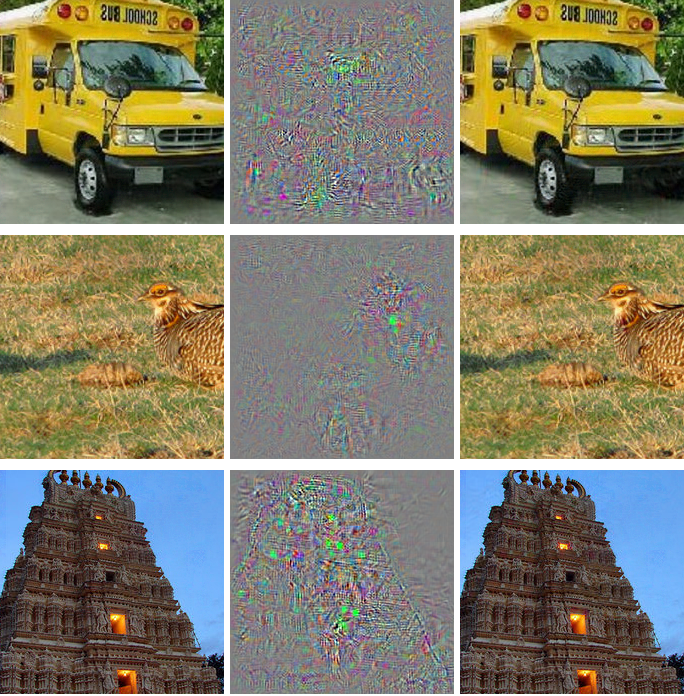
\includegraphics[width=7.3cm]{szegedy/negative1.png}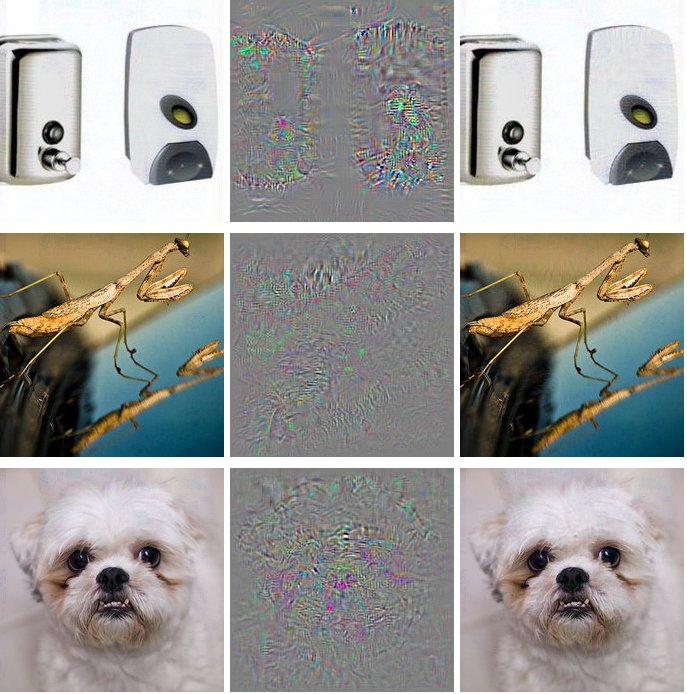
\includegraphics[width=7.3cm]{szegedy/negative2.png}
% %    \caption{Natural Images are in columns 1 and 4, Adversarial images are in columns 3 and 6, and the difference between them (magnified by a factor of 10) is in columns 2 and 5. All images in columns 3 and 6 are classified by AlexNet as "Ostrich" \cite{Szegedy2013}}
% %    \label{fig:my_label}
% %\end{figure}



% %The Dataset used above is known as ImageNet -- a large set of labeled images varying in size originally compiled for the ImageNet Large Scale Visual Recognition Challenge (ILSVRC). This dataset and its many subsets has become a standard for image classification and feature identification experiments. In the experiments that follow, ImageNet will be featured alongside the Modified National Institute of Standards and Technology (MNIST) dataset which is a database of hand written digits often used to develop image processing and character recognition systems. This dataset is much lower resolution than ImageNet and is therefore experiments run much more quickly on it and require less complex input/output.  

\section{Motivation and related work}

Our work is intended to shed light on the existence and prevalence of adversarial examples to DNN classifiers. It is closely related to other attempts to characterize robustness to adversarial perturbations, and here we give a detailed comparison.






%In the Sections \ref{sec:stab} and \ref{sec:experiments}, we will investigate stability of both natural data and adversarial examples in an attempt to understand how these different sets lie in the domain of the classifier. Understanding these geometries is a challenge for several reasons. For one, the data lies in a high dimensional space and thus the decision boundaries between classes are complicated submanifolds. Distances in high dimensional spaces are difficult to work with and do not always yield useful information. In particular, uniform distributions on balls in high dimensions often result in surprising results \citep{aggsurprising}. Instead, we consider high dimensional Gaussian distributions, using the variance as an alternative to distance. \citet{roth19aodds} and \citet{hosseini2019odds} take a similar approach, considering Gaussian noise perturbations of $\varepsilon$ times a vector with normal distribution $N(0,I)$. We describe their work below but note that they do not take advantage of using the variance to probe distributions which are more or less concentrated near their means.


%DG: moved to introduction Adversarial examples occur when natural data are close enough to the decision boundary that they can be imperceptibly perturbed to another class. Adversarial examples are not just a peculiarity, but seem to occur for most if not all DNN classifiers. \citet{inevitable2018} use isoperimetric inequalities on high dimensional spheres and hypercubes to conclude that there is a reasonably high probability that a correctly classified data point has a nearby adversarial example. \citet{ilyas2019adversarial} show that adversarial examples can arise from features that are good for classification but not robust to perturbation.

%{\bf Properties of the decision boundary.}
%data manifold, curvature of the decision boundary


{\bf Distance-based robustness.}
%Since we expect adversarial examples to exist, an important question is whether we can define a classifier to be robust to perturbations that might shift a natural example to an adversarial example. 
A typical approach to robustness of a classifier is to consider distances from the data manifold to the decision boundary ~\cite{Wang2020Improving, xu2023exploring, he2018decision}.  \citet{Khoury2018} define a classifier to be robust if the class of each point in the data manifold is contained in a sufficiently large ball that is entirely contained in the same class. The larger the balls, the more robust the classifier. It is then shown that if training sets are sufficiently dense in relation to the reach of the decision axis, the classifier will be robust in the sense that it classifies nearby points correctly. In practice, we do not know that the data is so well-positioned, and it is quite possible, especially in high dimensions, that the reach is extremely small, as evidenced by results on the prevalence of adversarial examples, e.g., \cite{inevitable2018} and in evaluation of ReLU networks with mixed integer linear programming e.g., ~\cite{tjeng2017evaluating}.

\citet{tsipras2018robustness} investigated robustness in terms of how small perturbations affect the the average loss of a classifier. They define standard accuracy of a classifier in terms of how often it classifies correctly, and robust accuracy in terms of how often an adversarially perturbed example classifies correctly. It was shown that sometimes accuracy of a classifier can result in poor robust accuracy. \citet{gilmer2018adversarial} use the expected distance to the nearest different class (when drawing a data point from the data distribution) to capture robustness, and then show that an accurate classifier can result in a small distance to the nearest different class in high dimensions when the data is drawn from concentric spheres. May recent works ~\cite{he2018decision, chen2023aware, jin2022roby} have linked robustness with decision boundary dynamics, buth by augmenting training with data near decision boundaries, or with dynamics related to distances from decision boundaries. We acknowledge the validity of this work, but will address some of its primary limitations by carefully studying the dynamics and orientation of the decision boundary relative to model data. 
A related idea is that adversarial examples often arise within cones, outside of which images are classified in the original class, as observed by \citet{roth19aodds}. Many theoretical models of adversarial examples, for instance the dimple model developed by \citet{shamir2021}, have high curvature and/or sharp corners as an essential piece of why adversarial examples can exists very close to natural examples.

% \textbf{Boundary Works}
% \begin{enumerate}[1.]
% % boundary work
% \item Improving Adversarial Robustness Requires Revisiting Misclassified Examples ~\cite{wang2020improving}
% \item Decision Boundary Analysis of Adversarial Examples ~\cite{he2018decision}
% \item Exploring and Exploiting Decision Boundary Dynamics for Adversarial Robustness ~\cite{xu2023exploring}
% \item Decision Boundary-Aware Data Augmentation for Adversarial Training ~\cite{chen2023aware}
% \item ROBY: Evaluating the adversarial robustness of a deep model by its decision boundaries ~\cite{jin2022roby} % these are all talking about distance to decision boundaries, not angles
% \end{enumerate}

{\bf Adversarial detection via sampling.}
While adversarial examples often occur, they still may be rare in the sense that most perturbations do not produce adversarial examples. \citet{yu2019new} used the observation that adversarial examples are both rare and close to the decision boundary to detect adversarial examples. They take a potential data point and look to see if nearby data points are classified differently than the original data point after only a few iterations of a gradient descent algorithm. If this is true, the data point is likely natural and if not, it is likely adversarial. This method has been generalized with the developing of smoothed classification methods (~\cite{cohen2019certified}, ~\cite{lecuyer2019certified}, ~\cite{li2019certified}) which at varying stages of evaluation add noise to the effect of smoothing output and identifying adversaries due to their higher sensitifity to perturbation.. These methods suffer from significant computational complexity ~\cite{kumar2020curse} and have been shown to have fundamental limitations in their ability to rigorously certify robustness (~\cite{blum2020random}, ~\cite{yang2020randomized}) we will generalize this approach into a metric which will allow us to directly study these limitations in order to better understand how geometric properties have given rise to adversarial vulnerabilities. In general, the results of \citet{yu2019new} indicate that considering samples of nearby points, which approximate the computation of integrals, is likely to be more successful than methods that consider only distance to the decision boundary.

%The goal would be to either develop a classifier robust to adversarial examples or to identify adversarial examples as opposed to natural data.

%DG: Moved to introduction. There have been many attempts to identify adversarial examples using properties of the decision boundary. \citet{Fawzi2018empirical} found that decision boundaries tend to have highly curved regions, and these regions tend to favor negative curvature, indicating that regions that define classes are highly nonconvex. These were found for a variety of DNNs and classification tasks. They also suggest exploiting this curvature discrepancy to identify when a data point is a natural image and when it is adversarial. It is also suggested that adversairal examples often arise within a cone, outside of which images are classified in the original class, as observed by \citet{roth19aodds} and as part of the dimple model theorized by \citet{shamir2021}.



\citet{roth19aodds} proposed a statistical method to identify adversarial examples from natural data. Their main idea was to consider how the last layer in the neural network (the logit layer) would behave on small perturbations of a natural example. %, i.e., on $x+\varepsilon n$ where $x$ is a natural example, $\varepsilon>0$ is small, and $n \sim N(0,I)$.  
This is then compared to the behavior of a potential adversarial example. 
% If it differs by a predetermined threshold, the example is flagged as adversarial. Successfully flagging adversarial examples in this way works best when adversarial examples tend to perturb toward the original class from which the adversarial example was perturbed. However, this is not always the case.
It was shown by \citet{hosseini2019odds} that it is possible to produce adversarial examples, for instance using a logit mimicry attack, that instead of perturbing an adversarial example toward the true class, actually perturb to some other background class. In fact, we will see in Section \ref{sec:mnist} that the emergence of a background class, which was observed as well by \citet{roth19aodds}, is quite common. Although many recent approaches have taken advantage of these facts ~\cite{taori2020shifts, lu2022randommasking, Osada_2023_WACV, blau2023classifier} in order to measure and increase robustness, we will leverage these sampling properties to develop a metric directly on decision-boundary dynamics and how they relate to the success of smoothing based robustness. 

% \textbf{Old Smoothing Works}
% \begin{enumerate}[1.]
% \item [A] Certified adversarial robustness via randomized smoothing, ICML 2019 ~\cite{cohen2019certified} 
% \item [B] Certified robustness to adversarial examples with differential privacy, SSP 2019 ~\cite{lecuyer2019certified} 
% \item [C] Certified adversarial robustness with additive noise, NeurIPS 2019 ~\cite{li2019certified}.

% Limitations And Societal Impact:
% The paper fails to discuss limitations and potential negative societal impact of the work. One limitation of "Gaussian-sampling based method" like in this work is that the method provably suffers from dimension curse for $L_{\text{infty}}$ adversarial attack. See [4-6].
% \item [D] Random Smoothing might be unable to certify $L^{\infty}$ Robustness for High-dimensional Images JMLR 2020 ~\cite{blum2020random}

% \item [E] Randomized smoothing of all shapes and sizes, ICML 2020 ~\cite{yang2020randomized} 
% \item [F] Curse of dimensionality on randomized smoothing for certifiable robustness, ICML 2020 ~\cite{kumar2020curse}.
% \end{enumerate}

% \textbf{Recent Perturbation/Smoothing Works}
% \begin{enumerate}[1.]
% % latest perturbation methods
% \item Unlabeled Data Improves Adversarial Robustness ~\cite{carmon2019unlabeled}
% \item Measuring Robustness to Natural Distribution Shifts in Image Classification ~\cite{taori2020shifts}
% \item MR2D: Multiple Random Masking Reconstruction Adversarial Detector ~\cite{lu2022randommasking}
% \item Out-of-Distribution Detection With Reconstruction Error and Typicality-Based Penalty ~\cite{Osada_2023_WACV}
% \item Classifier Robustness Enhanced via Test Time Transformation ~\cite{blau2023classifier}

% \end{enumerate}
% % other more recent lit  review. 

%DG: Mostly moved to introduction. \citet{roth19aodds} propose a statistical method to identify adversarial examples from natural data. Their main idea is to consider how the last layer in the neural network (the logit layer) would behave on a natural example with a small Gaussian perturbation, i.e., on $x+\varepsilon n$ where $x$ is a natural example, $\varepsilon>0$ is small, and $n \sim N(0,I)$.  This is then compared to the behavior of a potential adversarial example. If it differs by a predetermined threshold, the example is flagged as adversarial. Successfully flagging adversarial examples in this way is predicated on the hypothesis that adversarial examples tend to perturb toward the true class that they have been perturbed from. It is shown by \citet{hosseini2019odds} that it is possible to produce adversarial examples, for instance using a logit mimicry attack, that instead of perturbing an adversarial example toward the true class, actually perturb to some other background class. 
%In fact, we will see in Section \ref{sec:mnist} that the emergence of a background class, which was observed as well by \citet{roth19aodds}, is quite common. 

%This behavior will be observed in the case of classifiers of the MNIST digits dataset.

% Whereas \citet{roth19aodds} consider adding various types of noise to a given point and \citet{hosseini2019odds} consider small Gaussian perturbations of $x$ sampled from $N(x,\varepsilon^2 I)$ for small $\varepsilon$, %\todo{[K]: Should we go ahead and just be clear here and say $N(x,\varepsilon^2 I)$?} %noise perturbations of $\varepsilon$ times a vector with normal distribution $N(0,I)$ with a small selection of choices for $\varepsilon.$
% we specifically focus on %Our choice to consider varying standard deviations is quite similar to considering varying choices of $\varepsilon$ in the latter, but our focus is on 
% tuning the standard deviation parameter to determine a statistic describing how a given data point is placed within its class. The $\gamma$-persistence then gives a measurement similar to distance to the boundary but that is drawn from sampling instead of distance. The sampling allows for a better description of the local geometry of the class and decision boundary, as we will see in Section \ref{sec:stab}. Our statistic is based on the fraction of a Gaussian sampling of the neighborhood of a point which receives the same classification; this is different from that of \citet{roth19aodds}, which is the expected difference of the output of the logit layer of the original data point and the output of the logit layer for perturbed data points.  Additionally, while their statistics are defined pairwise with reference to pre-chosen original and candidate classes, ours is not.


%The focus of this particular paper is choosing that length apprWe instead consider perturbations of the form $N(0,\sigma^2 I)$ and vary $\sigma$. Each of these methods will perturbations with the same average length if $\varepsilon=\sigma$, but the latter will provide a greater spread of values for the length of the perturbations.

%The main reason\todo{[DG]: Yes, this needs to be moved. [K]: Yeah, but they are using Gaussians too, so I don't understand this comment about uniform distributions..} is that high dimensional Gaussian distributions are generally better behaved than uniform distributions on balls in high dimensions \citep{aggsurprising}. In addition, instead of just testing for various choices of the parameter, we find the parameter value for which the expectation of having a different result is above a certain threshold.

% \citet{yu2019new} observed that adversarial examples are a problem both because many are close to the decision boundary and they are rare. They use these almost contradictory observations to detect adversarial examples by taking a potential datapoint and looking to see if there are contra-classfied points (i.e., points classified different than the original datapoint) nearby that can be reached by only a few iterations of a gradient descent algorithm. If this is true, the datapoint is likely natural and if not, it is likely adversarial. The algorithm uses cutoff points based on previous understanding of the data. 

{\bf Manifold Aware Robustness}
% \subsection{Certified Robustness}

% Recently, there has been a push to develop methods which can certify the robustness of a model under certain constraints.
% These methods often involve classifying a neighborhood around a given sample.
% Some techniques use Monte-Carlo estimation \citep{cohen2019certified}, while others use abstraction to verify output bounds \citep{tjeng2017evaluating, singh2018fast}.
% While these methods are robust to attacks, they significantly increase inference cost.
% In an ideal case, we would like to make robustness claims about the entire input space rather than local areas around specific samples.
% ABOVE SENTENCE - could use expansion, there is a lot to unpack there and it is almost a claim, so we should use caution and be clear.
% There have been several attempts to explain this phenomenon.

% FOLLOW ON STATEMENT NEEDED HERE TO BRIDGE/END SECTION

% TODO: SOMETHING WITH THESE CITATIONS?

% Training models to be robust to multiple types of perturbations simultaneously \cite{tramer2019adversarial} % multiple perturbations
% TODO: Need more robust training papers

% \subsection{Saliency}

% The input gradients of discriminative models have been studied as a method of model explainability.
% The magnitude of these input gradients is often used as a fundamental feature attribution technique \cite{baehrens2010explain, simonyan2013deep}.
% Recent work demonstrates that many saliency methods fail basic sanity checks which should be expected out of explanation methods \citep{adebayo2018sanity, kindermans2019reliability}.
% The majority of these methods are build on careful measurement of input gradients.
% \citet{shah2021input} show that input gradient magnitude is not a consistent measure of feature attribution for standard models.
% In contrast, they show evidence that the input gradients of robust models are useful for feature attribution.
% This property of robust models is still not fully understood, however some hypotheses attempt to explain the relationship between robustness and PAG.
% The dimpled manifold hypothesis \citep{shamir2021dimpled} claims that images lie on some low-dimensional manifold, and model decision boundaries 'dimple' around individual data points.
% There also exists the hypothesis that there exist 'brittle' and 'robust' features in natural data and adversarial training forces a model to only focus on robust features \cite{ilyas2019adversarial, tsipras2018robustness}.


% \subsection{Manifold Alignment}

The sensitivity of convolutional neural networks to imperceptible changes in input has thrown into question the true generalization of these models.
Jo \& Bengio study the generalization performance of CNNs by transforming natural image statistics \cite{jo2017measuring}.  % surface level irregularities
Similarly to our MAG approach, they create a new dataset with well-known properties to allow the testing of their hypothesis.
They show that CNNs focus on high level image statistics rather than human perceptible features.
This problem is made worse by the fact that many saliency methods fail basic sanity checks \citep{adebayo2018sanity, kindermans2019reliability}.
% It has been hypothesized that removing texture bias from CNNs would alleviate this problem and improve robustness \citep{geirhos2018imagenet}. % texture bias
Until recently, it was unclear whether robustness and manifold alignment were directly linked, as the only method to achieve manifold alignment was adversarial training.
Along with the discovery that smoothed classifiers are perceptually aligned, comes the hypothesis that robust models in general share this property \cite{kaur2019perceptually}.
This discovery raises the question of whether this relationship is bidirectional.

Khoury \& Hadfield-Menell study the geometry of natural images, and create a lower bound for the number of data points required to cover the manifold \citet{khoury2018geometry}.
Unfortunately, they demonstrate that this lower bound is so large as to be intractable.
Shamir et al propose using the tangent space of a generative model as an estimation of this manifold \cite{shamir2021dimpled}. Magai et al. thoroughly review certain topological properties to demonstrate that neural networks intrinsically use relatively few dimensions of variation during training and evaluation ~\cite{magai2022topology}. Vardi et al. demonstrate that even models which satisfy strong conditions related to max margin classifiers are implicitly non-robust ~\cite{vardi2022gradient}. PCA and manifold metrics have been recently used to identify adversarial examples ~\cite{aparne2022pca, nguyen-minh-luu-2022-textual}. We will extend this work to study the relationship between robustness and manifold alignment directly by baking alignment directly into networks and comparing them with another approach to robustness. 
% Their work studies the geometry of natural images in an attempt to create a lower bound for the number of data points required to cover a natural image manifold.
% The property that every data point has a nearby adversarial point for every class is counter intuitive to the way we as humans imagine the decision boundaries of neural networks.



%Each of these works is predicated on understanding stability of natural and adversarial examples under Gaussian perturbations of the data. In this study, we look more closely at how such perturbations change classification. In the sequel, we will give a definition that is agnostic of choice of classifier, though we focus on different types of Neural Network based classifiers.

{\bf Summary.}
 In Sections \ref{sec:meth} and \ref{sec:experiments}, we will investigate stability of both natural data and adversarial examples by considering sampling from Gaussian distributions centered at a data point with varying standard deviations. Using the standard deviation as a parameter, we are able to derive a statistic for each point that captures how entrenched it is in its class in a way that is less restrictive than the robustness described by \citet{Khoury2018}, takes into account the rareness of adversarial examples described by \citet{yu2019new}, builds on the idea of sampling described by \citet{roth19aodds} and \citet{hosseini2019odds}, and represent curvatures in a sense related to \citet{Fawzi2018empirical}. Furthermore, we will relate these stability studies to direct measurement of interpolation incident angles with decision boundaries in Subsection~\ref{subsec:db} and ~\ref{subsec:dbe} and the effect of reduction of data onto a known lower dimensional manifold in Subsections ~\ref{subsec:ma} and ~\ref{subsec:mae}.  
 %The main contribution is the development of a precise notion of stability, called $(\gamma, \sigma)$-stability, and a statistic, called $\gamma$-persistence, that represent each of these notions in a quantitative, clear way. The methods use sampling of Gaussians, which is generally quite easy compared to other measures in high dimensions.  \todo{[DG]: we maybe want to add the reference \cite{creschi2019} to discuss using dimension reduction/t-SNE to capture manifold property of data and \cite{Lee2018ASU} with a method to detect out of manifold data for adversarial attacks} 


\section{Methods} \label{sec:meth} % Stability and Persistence

In this section we will lay out the theoretical framework for studying stability, persistence, and decision boundary corssing-angles. 

\subsection{Stability and Persistence} \label{subsec:stab}
In this section we define a notion of stability of classification of a point under a given classification model. In the following, $X$ represents the ambient space the data is drawn from (typically $\RR^n$) even if the data lives on a submanifold of $X$, and $L$ is a set of labels (often $\{1,\dots,\ell\}$).  Note that points $x\in X$ can be natural or adversarial points.%The following definition complements the definition for adversarial examples by providing a criteria for the local stability of the classifier about a point, which could be an actual test point or an adversarial example: 

\begin{definition}
Let $\CC:X\to L$ be a classifier, $x \in X$, $\gamma\in(0,1)$, and $\sigma>0$. We say $x$ is \emph{$(\gamma,\sigma)$-stable} with respect to $\CC$ if $\mathbb{P}[\CC(x')=\CC(x)] \geq \gamma$ for $x' \sim \rho = N(x, \sigma^2 I)$; i.e. $x'$ is drawn from a Gaussian with variance $\sigma^2$ and mean $x$.
\end{definition}

In the common setting when $X=\RR^n$, we have
\[\mathbb{P}[\CC(x')=\CC(x)] = \int_{\RR^n} \mathbbm{1}_{\CC^{-1}(\CC(x))} (x') d\rho (x') = \rho(\CC^{-1}\CC(x)).\]
Note here that $\CC^{-1}$ denotes preimage. %In the case of images drawn from $\RR^n$, we can write this integral precisely as
One could substitute various probability measures $\rho$ above with mean $x$ and variance $\sigma^2$ to obtain different measures of stability corresponding to different ways of sampling the neighborhood of a point.  Another natural choice would be sampling the uniform measure on balls of changing radius. Based on the concentration of measure for both of these families of measures we do not anticipate significant qualitative differences in these two approaches. We propose Gaussian sampling because it is also a product measure, which makes it easier to sample and simplifies some other calculations below.

For the Gaussian measure, the probability above may be written more concretely as
\begin{equation}\label{EQN:Gaussian}
\frac{1}{\left(\sqrt{2\pi}\sigma\right)^{n}} \int_{\RR^n} \mathbbm{1}_{\CC^{-1}(\CC(x))} (x')e^{-\frac{\norm{x - x'}^2}{2\sigma^2}} dx'.
\end{equation}
In this work, we will conduct experiments in which we estimate this stability for fixed $(\gamma,\sigma)$ pairs via a Monte Carlo sampling, in which case the integral \eqref{EQN:Gaussian} is approximated by taking $N$ i.i.d. samples $x_k \sim \rho$ and computing
\[
    \frac{\norm{x_k : \CC(x_k) = \CC(x)}}{N}.
\]
Note that this quantity converges to the integral \eqref{EQN:Gaussian} as $N\to\infty$ by the Law of Large Numbers.

The ability to adjust the quantity $\gamma$ is important because it is much weaker than a notion of stability that requires a ball that stays away from the decision boundary as in \cite{Khoury2018}. By choosing $\gamma$ closer to $1$, we can require the samples to be more within the same class, and by adjusting $\gamma$ to be smaller we can allow more overlap.

We also propose a related statistic, \emph{persistence}, by fixing a particular $\gamma$ and adjusting $\sigma$. For any $x\in X$ not on the decision boundary, for any choice of $0<\gamma<1$ there exists a $\sigma_\gamma$ small enough such that if $\sigma < \sigma_\gamma$ then $x$ is $(\gamma,\sigma)$-stable. We can now take the largest such $\sigma_\gamma$ to define persistence.

%In our experiments, $\gamma$ is fixed and $\sigma$ is adjusted to determine the largest $\sigma$ for which an image is $(\gamma,\sigma)$-stable.  We define this to be persistence as follows.


\begin{definition}
    Let $\CC:X\to L$ be a classifier, $x \in X$, and $\gamma\in(0,1)$. Let $\sigma_\gamma^*$ be the maximum $\sigma_\gamma$ such that $x$ is $(\gamma, \sigma)$-stable with respect to $\CC$ for all $\sigma<\sigma_\gamma$. We say that $x$ has \emph{$\gamma$-persistence} $\sigma_\gamma^*$.
\end{definition}

The $\gamma$-persistence quantity $\sigma_\gamma^*$ measures the stability of the neighborhood of a given $x$ with respect to the output classification. Small persistence indicates that the classifier is unstable in a small neighborhood of $x$, whereas large persistence indicates stability of the classifier in a small neighborhood of $x$. In the later experiments, we have generally taken $\gamma = 0.7$. This choice is arbitrary and chosen to fit the problems considered here. In our experiments, we did not see significant change in results with small changes in the choice of $\gamma$.



%It follows that if we fix the distance $d$ to the decision boundary, the more planes making up the decision boundary, the smaller the persistence will be. For instance, in the case of $d=1$ and a single hyperplane decision boundary, the $0.7$-persistence is approximately $1.91$, whereas a two hyperplane decision boundary has $0.7$-persistence of approximately $1.02$ and a three hyperplane decision boundary has $0.7$-persistence of approximately $0.82$. Note that if the initial point is outside the cone, then the persistence will be significantly larger. This demonstrates how, even if we consider points equally close to the decision boundary, the persistence can distinguish between being in a location that is inside a cone and outside a cone, as well as how sharp the boundary of those cones may be. The existence of such cones or curved decision boundaries is both seen experimentally \citep{Fawzi2018empirical,roth19aodds} and theorized \citep{shamir2021}.



In our experiments, we numerically estimate $\gamma$-persistence via a bisection algorithm that we term the Bracketing Algorithm.  Briefly, the algorithm first chooses search space bounds $\sigma_{\min}$ and $\sigma_{\max}$ such that $x$ is  $(\gamma,\sigma_{\min})$-stable but is not $(\gamma,\sigma_{\max})$-stable with respect to $\CC$, and then proceeds to evaluate stability by bisection until an approximation of $\sigma_\gamma^*$ is obtained.


%This is accomplished by a bracketing procedure: we first expand the search space bounds $\sigma_{\min}$ and $\sigma_{\max}$ so that the average number of samples at these bounds are below (respectively above) $\gamma$.  This search space is then sequentially bisected to identify a $\sigma$ corresponding with $\gamma$ (the full algorithm is presented in the Appendix).

%We can compute approximate the $\gamma$-persistence using a bisection algorithm we call the Bracketing Algorithm. The Bracketing Algorithm is given as Algorithm \ref{bracketing} in Appendix \ref{sec:bracketing}.  

%\renewcommand{\baselinestretch}{1.0}

%\renewcommand{\baselinestretch}{1.5}
\subsection{Decision Boundaries} \label{subsec:db}

In order to examine decision boundaries and their properties, we will carefully define the decision boundary in a variety of equivalent formulations. 

\subsubsection{The Argmax Function Arises in Multi-Class Problems}

A central issue when writing classifiers is mapping from continuous outputs or probabilities to discrete sets of classes. Frequently argmax type functions are used to accomplish this mapping. To discuss decision boundaries, we must precisely define argmax and some of its properties. 

In practice, argmax is not strictly a function, but rather a mapping from the set of outputs or activations from another model into the power set of a discrete set of classes:

\begin{equation}
    \text{argmax} : \R^k \to \mathcal{P}(C)
\end{equation}

Defined this way, we cannot necessarily consider $\text{argmax}$ to be a function in general as the singleton outputs of argmax overlap in an undefined way with other sets from the power set. However, if we restrict our domain carefully, we can identify certain properties. 
\begin{figure}[!ht]
\begin{center}
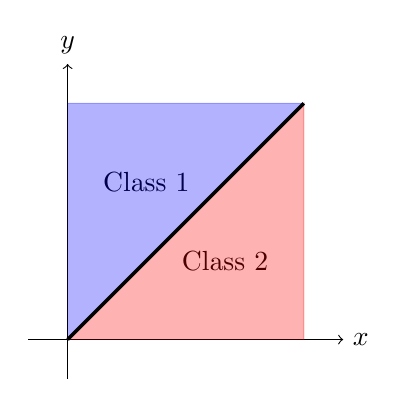
\begin{tikzpicture}
  \draw[->] (-0.5, 0) -- (3.5, 0) node[right] {$x$};
  \draw[->] (0, -0.5) -- (0, 3.5) node[above] {$y$};
  \node at (1, 2) (c1) {Class 1};
  \node at (2, 1) (c2) {Class 2};
  \draw[-, fill, blue, opacity=.3] (0, 3) -- (3, 3) -- (0, 0);
  \draw[-, fill, red, opacity=.3] (3, 0) -- (3, 3) -- (0, 0);
  \draw[scale=1, domain=0:3, smooth, variable=\x, black, line width=0.45mm] plot ({\x}, {\x});
  %\draw[scale=0.5, domain=-3:3, smooth, variable=\y, red]  plot ({\y*\y}, {\y});
\end{tikzpicture}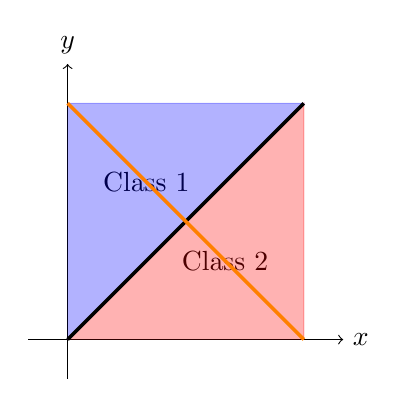
\begin{tikzpicture}
  \draw[->] (-0.5, 0) -- (3.5, 0) node[right] {$x$};
  \draw[->] (0, -0.5) -- (0, 3.5) node[above] {$y$};
  \node at (1, 2) (c1) {Class 1};
  \node at (2, 1) (c2) {Class 2};
  \draw[-, fill, blue, opacity=.3] (0, 3) -- (3, 3) -- (0, 0);
  \draw[-, fill, red, opacity=.3] (3, 0) -- (3, 3) -- (0, 0);
  \draw[scale=1, domain=0:3, smooth, variable=\x, black, line width=0.45mm] plot ({\x}, {\x});
  \draw[-, orange, line width=0.45mm] (0,3) -- (3, 0);
  %\draw[scale=0.5, domain=-3:3, smooth, variable=\y, red]  plot ({\y*\y}, {\y});
\end{tikzpicture}

\caption{Decision boundary in $[0,1] \times [0,1]$ (left) and decision boundary restricted to probabilities (right) If the output of $F$ are \emph{probabilities} which add to one, then all points of $x$ will map to the orange line on the right side of Figure~\ref{fig:pdb}. We note that the point $(0.5, 0.5)$ is therefore the only point on the decision boundary for probability valued $F$. We may generalize to higher dimensions where all probability valued models $F$ will map into the the plane $x + y + z + \cdots = 1$ in $Y$ and the decision boundary will be partitioned into $K-1$ components, where the $K$-decision boundary is the intersection of this plane with the \emph{centroid} line $x = y = z = \cdots$ and the $2$-decision boundaries become planes intersecting at the same line. }
\label{fig:pdb}
\end{center}
\end{figure}
Restricting to only the pre-image of the singletons, it should be clear that argmax is continuous.  Indeed, restricted to the pre-image of any set in the power-set, argmax is continuous. Further, we can directly prove that the pre-image of an individual singleton is open. Observe that for any point whose image is a singleton, one element of the domain vector must exceed the others by $\varepsilon > 0$. We shall use the $\ell^1$ metric for distance, and thus if we restrict ourselves to a ball of radius $\varepsilon$, then all elements inside this ball will have that element still larger than the rest and thus map to the same singleton under argmax. Since the union of infinitely many open sets is open in $\R^k$, the union of all singleton pre-images is an open set. Conveniently this also provides proof that the union of all of the non-singleton sets in $\mathcal{P}(C)$ is a closed set. We will call this closed set the argmax Decision Boundary. We will list two equivalent formulations for this boundary. 

% \subsubsection{Defining Decision Boundaries}

\paragraph{Complement Definition}

A point $x$ is in the \emph{decision interior} $D_f'$ for a classifier $f: \mathbb{R}^N -> \mathcal{C}$ if there exists $\delta > 0$ such that $\forall \epsilon < \delta$, $|f(B_\epsilon(x))| = 1$. 

The \emph{decision boundary} of a classifier $f$ is the closure of the complement of the decision interior $\overline{\{x : x \notin D_f'\}}$. 

% \paragraph{Constructive Definition}

% A point $x$ is on the \emph{decision boundary} $D$ of a classifier $F = f \circ \argmax$ if $\forall \epsilon > 0$, $|f(B_\epsilon(x))| \geq 2$.\\

% A point $x$ is a \emph{binary decision point} if $\exists \delta > 0$ such that $\forall \epsilon > 0$ if $\epsilon < \delta$, then $|f(B_\epsilon(x))| = 2$. 

% A point $x$ is on the \emph{$K$-decision boundary} $D^K$ of a classifier $f$ if $\exists \delta > 0$ such that $\forall \epsilon > 0$ if $\epsilon < \delta$, then $|f(B_\epsilon(x))| = K$. 

\paragraph{Level Set Definition}

The decision boundary $D$ of a probability valued function $f$ is the pre-image of a union of all level sets of activations $A_c = {c_1, c_2, ..., c_k}$ defined by a constant $c$ such that for some set of indices $L$, we have $c = c_i$ for every $i$ in $L$ and $c > c_j$ for every $j$ not in $L$. The pre-image of each such set are all $x$ such that $f(x) = A_c$ for some $c$. 



\section{Experiments} \label{sec:experiments}

%???Did we try Carlini-Wagner method? -- B2 not yet, working on it for Imnet

% B2 -- here's what we have ready to go

In this section we investigate the stability and persistence behavior of natural and adversarial examples for MNIST \citep{MNIST} and ImageNet \citep{ILSVRC15} using a variety of different classifiers. For each set of image samples generated for a particular dataset, model, and attack protocol, we study $(\gamma,\sigma)$-stability and $\gamma$-persistence of both natural and adversarial images, and also compute persistence along trajectories from natural to adversarial images. In general, we use $\gamma = 0.7$, and note that the observed behavior does not change significantly for small changes in $\gamma$. While most of the adversarial attacks considered here have a clear target class, the measurement of persistence does not require considering a particular candidate class.  Furthermore, we will evaluate decision boundary incidence angles and apply our conclusions to evaluate models trained with manifold aligned gradients. 




% Adversarial examples are generated using Iterative Gradient Sign Method (IGSM) \citep{kurakin_adversarial_2016}, which is an iterative version of the Fast Gradient Sign Method (FGSM) \cite{goodfellow_explaining_2014}, as well as the more primitive Limited-memory Broyden-Fletcher-Goldfarb-Shanno (L-BFGS) optimization algorithm \citep{liu1989limited}. 

% The neighborhoods around datapoints and adversarial examples are sampled using Gaussians with varying standard deviation $\sigma$, and Algorithm \ref{bracketing} is used to approximate $\gamma$-persistence corresponding to $\gamma=0.7$. The resultant $0.7$-persistence $\sigma_{.7}^*$ statistically identifies examples as being $(0.7,\sigma_{.7}^*)$-stable, meaning that 70\% of the samples drawn from a Gaussian with standard deviation $\sigma$ are classified the same as the original class by the model. 

% The first test of the ideas behind $(\gamma, \sigma)$-stability is to consider what happens to Gaussian samples as the standard deviation is increased from zero. To this end, for each choice of $\sigma$ ??Where?? we took 1000 samples around the original image or adversarial image and plotted the count of how many were classified with each label. These results are seen in Figures ???? %Algorithm \ref{bracketing} is used to approximate $\gamma$-persistence corresponding to $\gamma=0.7$. The resultant $0.7$-persistence $\sigma$ statistically identifies examples as being $(0.7,\sigma)$-stable, meaning that 70\% of the samples drawn from a Gaussian with standard deviation $\sigma$ are classified the same as the original class by the model. 
% In order to understand the impact of model complexity on $(\gamma, \sigma)$-stability of adversarial examples, we considered the framework of \citet{Szegedy2013}, looking at a variety of networks of differing complexities, including both fully-connected and convolutional neural networks.


\subsection{MNIST Experiments}

%The MNIST dataset consists of 28 by 28 pixels, so it can naturally be considered as a data set on a 784 dimensional vector space. The size of this data makes it ideal for initial testing. 
Since MNIST is relatively small compared to ImageNet, we trained several classifiers with various architectures and complexities and implemented the adversarial attacks directly. Adversarial examples were generated against each of these models using Iterative Gradient Sign Method (IGSM \citep{kurakin_adversarial_2016}) and Limited-memory Broyden-Fletcher-Goldfarb-Shanno (L-BFGS \citep{liu1989limited}).


 

\subsubsection{Investigation of $(\gamma, \sigma)$-stability on MNIST}\label{sec:mnist}

We begin with a fully connected ReLU network with layers of size 784, 100, 20, and 10 and small regularization $\lambda = 10^{-7}$ which is trained on the standard MNIST training set. We then start with a randomly selected MNIST test image $x_1$ from the \texttt{1}'s class and generate adversarial examples $x_0,x_2,\dots,x_9$ using IGSM for each target class other than \texttt{1}. The neighborhoods around each $x_i$ are examined by generating 1000 i.i.d. samples from $N(x_i,\sigma^2I)$ for each of 100 equally spaced standard deviations $\sigma\in(0,1.6)$. Figure \ref{fgsmo} shows the results of the Gaussian perturbations of a natural example $x_1$ of the class labeled \texttt{1} and the results of Gaussian perturbations of the adversarial example $x_0$ targeted at the class labeled \texttt{0}. We provide other examples of $x_2,\ldots,x_9$ in the supplementary materials. Note that the original image is very stable under perturbation, while the adversarial image is not. 

% \begin{figure}[ht]
% \includegraphics[trim=200 80 100 100, clip, width = .9\textwidth]
% %[trim=200 80 100 100, clip,width=15cm]
% {c3_figures/Image918-O1Anone_varx40.png}
% \caption{Frequency of each class in Gaussian samples with increasing variance around an adversarial image of a $1$ targeted at $0$ generated using IGSM. The adversarial class is shown as a red curve. The natural image class is shown in black. The bottom shows example sample images.}
% \label{fgsmo}
% \end{figure}


% \begin{figure}[ht]
% \includegraphics[trim=200 80 100 100,clip, width = .9\textwidth]
% %[trim=200 80 100 100, clip,width=15cm]
% {c3_figures/Image918-O1A0_varx40.png}
% \caption{Frequency of each class in Gaussian samples with increasing variance around an adversarial image of a $1$ targeted at $0$ generated using IGSM. The adversarial class is shown as a red curve. The natural image class is shown in black. The bottom shows example sample images. }
% \label{fgsma}
% \end{figure}

\begin{figure}[!ht]
\includegraphics[width = .49\textwidth]
%[trim=200 80 100 100, clip,width=15cm]
{c3_figures/MNIST1.png} \includegraphics[width = .49\textwidth]
%[trim=200 80 100 100, clip,width=15cm]
{c3_figures/MNIST10.png}
\caption{Frequency of each class in Gaussian samples with increasing variance around a natural image of class \texttt{1} (left) and around an adversarial attack of that image targeted at \texttt{0} generated using IGSM (right). The adversarial class (\texttt{0}) is shown as a red curve. The natural image class (\texttt{1}) is shown in black. Bottoms show example sample images at different standard deviations for natural (left) and adversarial (right) examples.}\label{fgsmo}
\end{figure}



\subsubsection{Persistence of adversarial examples for MNIST}

% For adversarial examples, we are particularly interested in comparing the classification counts around each example relative to the distortion ($\|x\|_2/\sqrt{n}$) introduced to generate the example. We then compute $0.7$-persistence for a variety of models and samples and summarize these results.

To study persistence of adversarial examples on MNIST, we take the same network architecture as in the previous subsection and randomly select 200 MNIST images. For each image, we used IGSM to generate 9 adversarial examples (one for each target class) yielding a total of 1800 adversarial examples. In addition, we randomly sampled 1800 natural MNIST images. For each of the 3600 images, we computed $0.7$-persistence; the results are shown in Figure \ref{fig:IGSMpersistenceMNIST}. One sees that $0.7$-persistence of adversarial examples tends to be significantly smaller than that of natural examples for this classifier, indicating that they are generally less stable than natural images. We will see subsequently that this behavior is typical.

%and generate adversarial examples using IGSM for each of 200 randomly selected MNIST images to each possible target other than the original class (9 total targets) for a total of 1800 adversarial examples. 
 %The images were processed using a bisection algorithm (Algorithm \ref{bracketing} in the supplementary materials) to compute $0.7$-persistence. The results are aggregated in Figure \ref{fig:IGSMpersistenceMNIST}.
\begin{figure}[!ht]
\centering
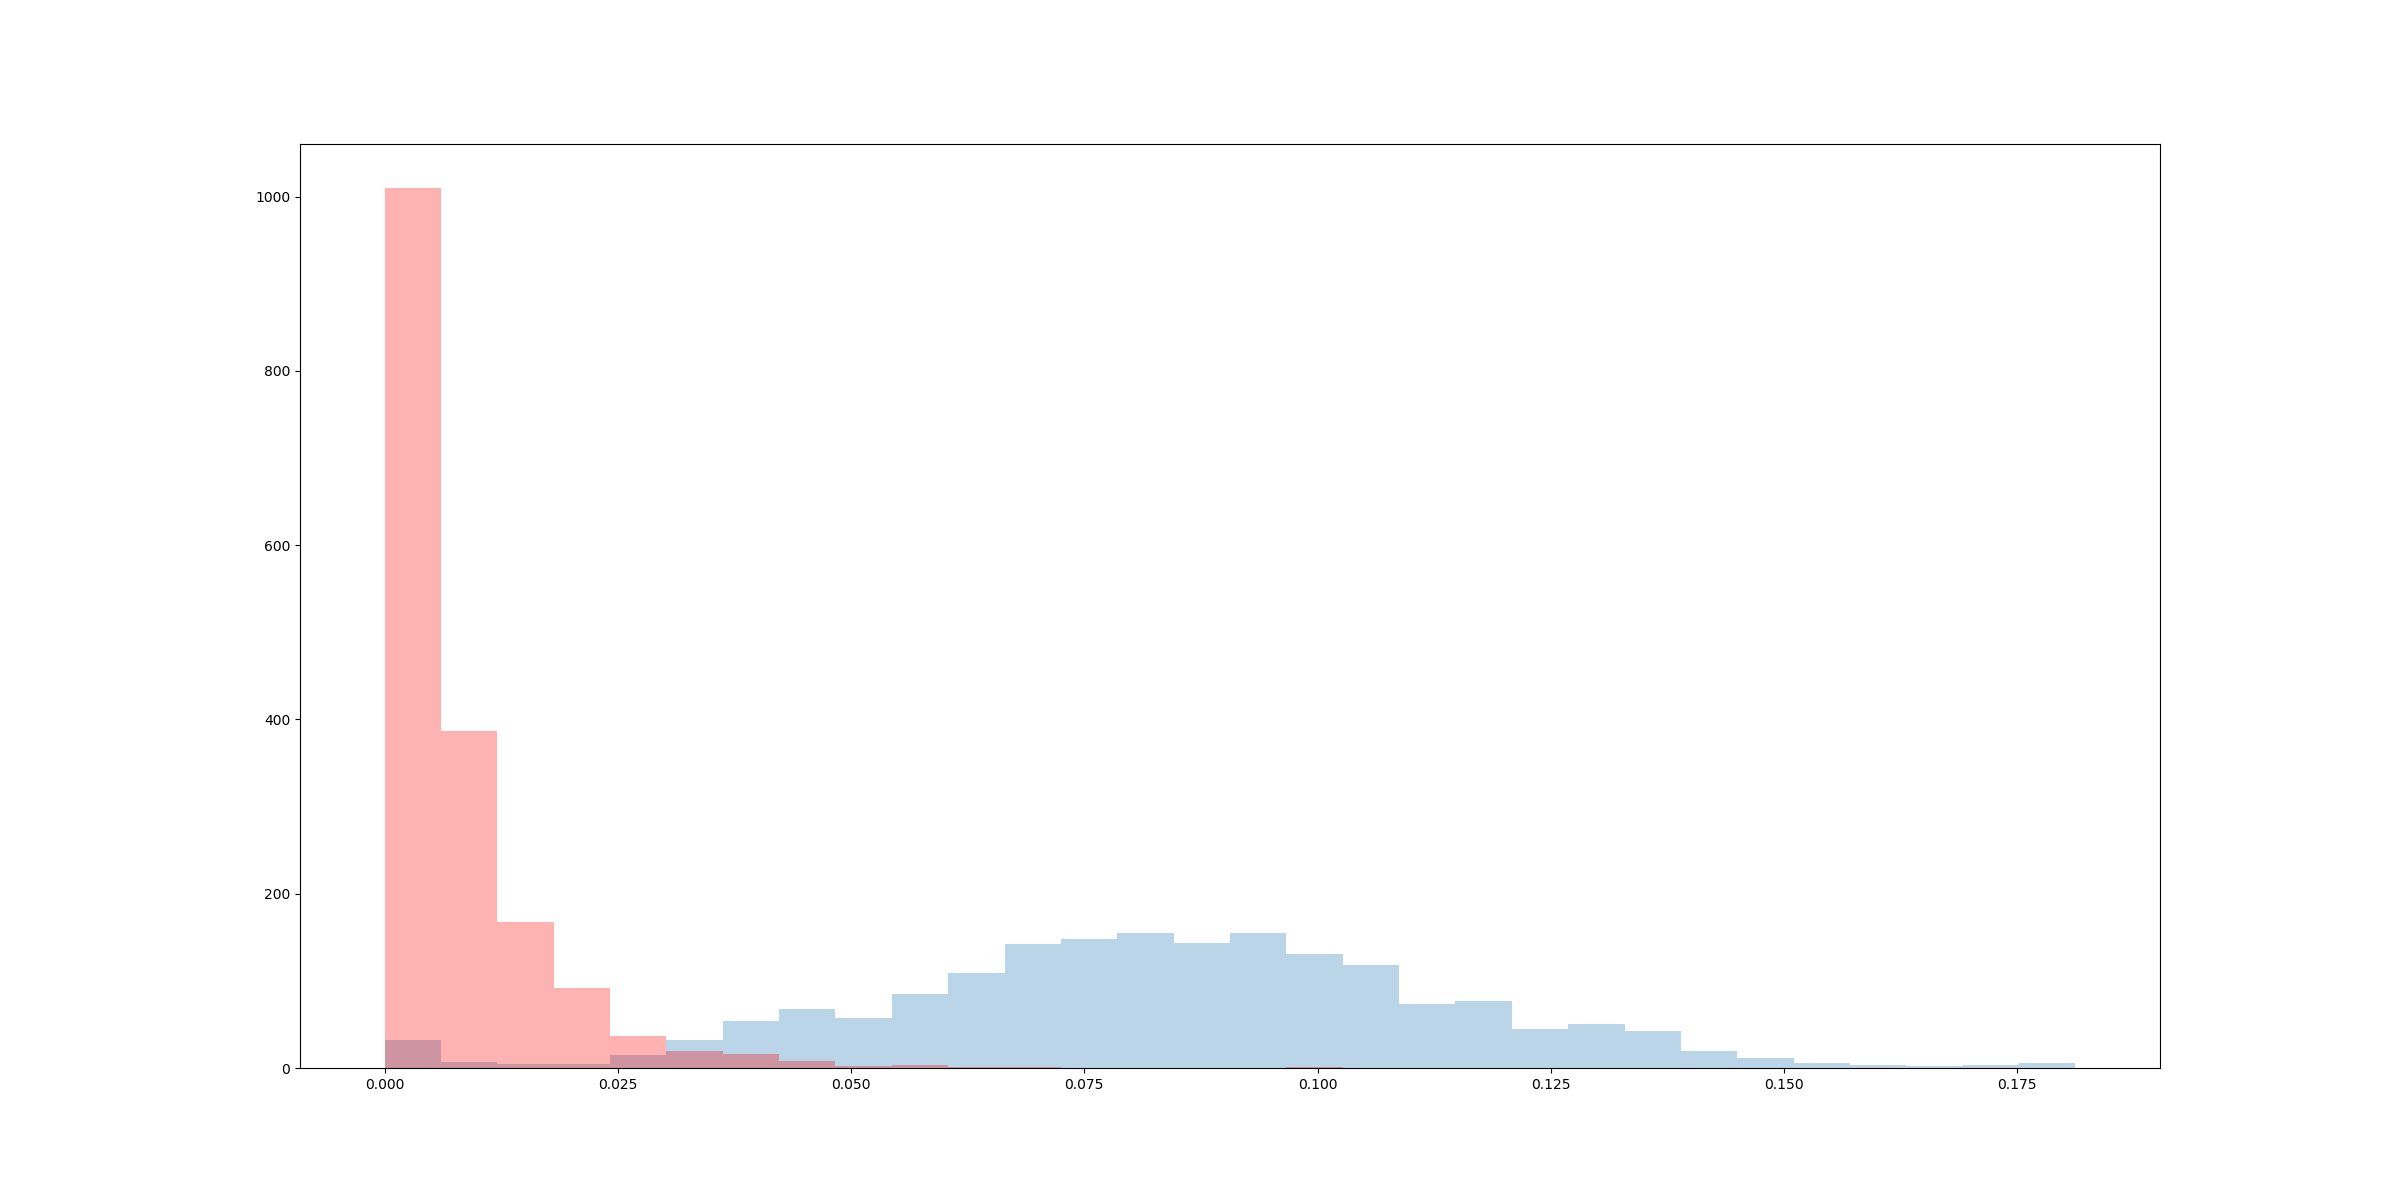
\includegraphics[trim=200 80 100 100, clip,width=.5\textwidth]{c3_figures/original_hist.png}
\caption{Histogram of $0.7$-persistence of IGSM-based adversarial examples (red) and natural examples (blue) on MNIST. %The histogram shows that $0.7$-persistence for adversarial examples tends to be smaller than $0.7$-persistence for natural examples.
}
%\label{fgsmh}
\label{fig:IGSMpersistenceMNIST}
\end{figure}
% TODO : expand figure 13 with a wide sample of adversarial versus natural examples from imagenet. 
%In this experiment, the adversarial examples (red) tended to have a lower $0.7$- persistence than natural images (blue), indicating that they were much less stable than the natural images. %DG: I HAVE REMOVED: We can define a linear classifier on these $\gamma$-persistence values which will identify adversarial attacks with 98\% accuracy. 

%\subsection{Effects of network complexity on persistence}
%{Neighborhood sampling of L-BFGS adversarial examples for MNIST}

Next, we investigate the relationship of network complexity and $(\gamma,\sigma)$-stability by revisiting the now classic work of \citet{Szegedy2013} on adversarial examples. 
%In these experiments, we used L-BFGS technique from \cite{Szegedy2013} to prepare adversarial examples. The same network architectures and examples were subjected to $0.7$-persistence analysis to determine the correspondence of stability with network accuracy and average distortion. In this case we will loosely define complexity as the effective number of parameters of a network and distortion is the $\ell^2$ norm divided by square root of the dimension $n$. 
%[??DG??: We need to define complexity and add it to the table]
%\subsubsection{Re-examining Szegedy Results with sampling}
%
Table \ref{table1} recreates and adds on to part of \cite[Table 1]{Szegedy2013} in which networks of differing complexity are trained and attacked using L-BFGS. The table contains new columns showing the average $0.7$-persistence for both natural and adversarial examples for each network, as well as the average distortion for the adversarial examples. The distortion is the $\ell^2$-norm divided by square root of the dimension $n$. The first networks listed are of the form FC10-k, and are fully connected single layer ReLU networks that map each input vector $x \in \RR^{784}$ to an output vector $y \in \RR^{10}$ with a regularization added to the objective function of the form $\lambda\Norm{w}_2/N$, where $\lambda = 10^{-k}$ and $N$ is the number of parameters in the weight vector $w$ defining the network. The higher values of $\lambda$ indicate more regularization.  
%added as regularization to the objective function during training. FC10-2 is the same except with $\lambda = 10^{-2}$ and FC10-0 has $\lambda=1$ (a very large coefficient for regularization). 
FC100-100-10 and FC200-200-10 are networks with 2 hidden layers (with 100 and 200 nodes, respectively) with regularization added for each layer of perceptrons with the $\lambda$ for each layer equal to $10^{-5}, 10^{-5}$, and  $10^{-6}$. Training for these networks was conducted with a fixed number of epochs (typically 21). For the bottom half of Table \ref{table1}, we also considered networks with four convolutional layers plus a max-pooling layer connected by ReLU to a fully connected hidden layer with increasing numbers of channels denoted as as ``C-Ch,'' where C reflects that this is a CNN and Ch denotes the number of channels. A more detailed description of these networks can be found in Appendix \ref{appendix:CNNs}.

\begin{table}[ht]
\centering
\caption{Recreation of \citet[Table 1]{Szegedy2013} for the MNIST dataset.  For each network, we show Testing Accuracy (in \%), Average Distortion ($\|x\|_2/\sqrt{n}$) of adversarial examples, and new columns show average $0.7$-persistence values for natural (Nat) and adversarial (Adv) images. 300 natural and 300 adversarial examples generated with L-BFGS were used for each aggregation.}
\label{table1}
\begin{tabular}{lllll}
\toprule
Network & Test Acc & Avg Dist & Persist (Nat) & Persist (Adv) \\
\midrule
FC10-4 & 92.09 & 0.123 & 0.93 & 1.68\\
FC10-2 & 90.77 & 0.178 & 1.37 & 4.25\\
FC10-0 & 86.89 & 0.278 & 1.92 & 12.22\\
FC100-100-10 & 97.31 & 0.086 & 0.65 & 0.56 \\
FC200-200-10 & 97.61 & 0.087 & 0.73 & 0.56 \\
\midrule
C-2 & 95.94 & 0.09 & 3.33 & 0.027 \\
C-4 & 97.36 & 0.12 & 0.35 & 0.027 \\
C-8 & 98.50 & 0.11 & 0.43  & 0.0517 \\
C-16 & 98.90 & 0.11 & 0.53 & 0.0994 \\
C-32 & 98.96 & 0.11 & 0.78 & 0.0836 \\
C-64 & 99.00 & 0.10 & 0.81 & 0.0865 \\
C-128 & 99.17 & 0.11 & 0.77 & 0.0883 \\
C-256 & 99.09 & 0.11  & 0.83 & 0.0900 \\
C-512 & 99.22 & 0.10 & 0.793 & 0.0929 \\
%C-128-2000 & 99.07 & 0.11 & 89.27 & 0.731 & 0.136 \\
%C-128-4000 & 99.13 & 0.098 & 89.71 & 1.024 & 0.424 \\
%C-128-4500 & 99.32 & 0.096 & 90.59 & NA & 0.103 \\
%C-128-4700 & 97.48 & 0.079 & 87.16 & NA & NA \\
%C-128-4708 & 95.69 & 0.077 & 80.90 & 0.15 & 0.0307 \\
%C-128-4712 & 93.04 & 0.135 & 57.11 & 0.14 & 0.0296 \\
%C-128-4714 & 78.87 & 0.211 & 41.61 & 0.059 & 0.012 \\
%C-128-4715 & 65.99 & 0.831 & 23.61 & NA & 0.0092 \\ \hline
\bottomrule
\end{tabular}
\end{table}

The main observation from Table \ref{table1} is that for higher complexity networks,
adversarial examples tend to have smaller persistence than natural examples. Histograms reflecting these observations can be found in the supplemental material. %This can be seen as well in Figure \ref{fig:FC200-200-10}, which shows the $0.7$-persistence for natural and adversarial examples for the network FC200-200-10. 
Another notable takeaway is that for models with fewer effective parameters, the attack distortion necessary to generate a successful attack is so great that the resulting image is often more stable than a natural image under that model, as seen particularly in the FC10 networks. Once there are sufficiently many parameters available in the neural network, we found that both the average distortion of the adversarial examples and the average $0.7$-persistence of the adversarial examples tended to be smaller. This observation is consistent with the idea that networks with more parameters are more likely to exhibit decision boundaries with more curvature.

% \begin{figure}[h!]
% \centering
% 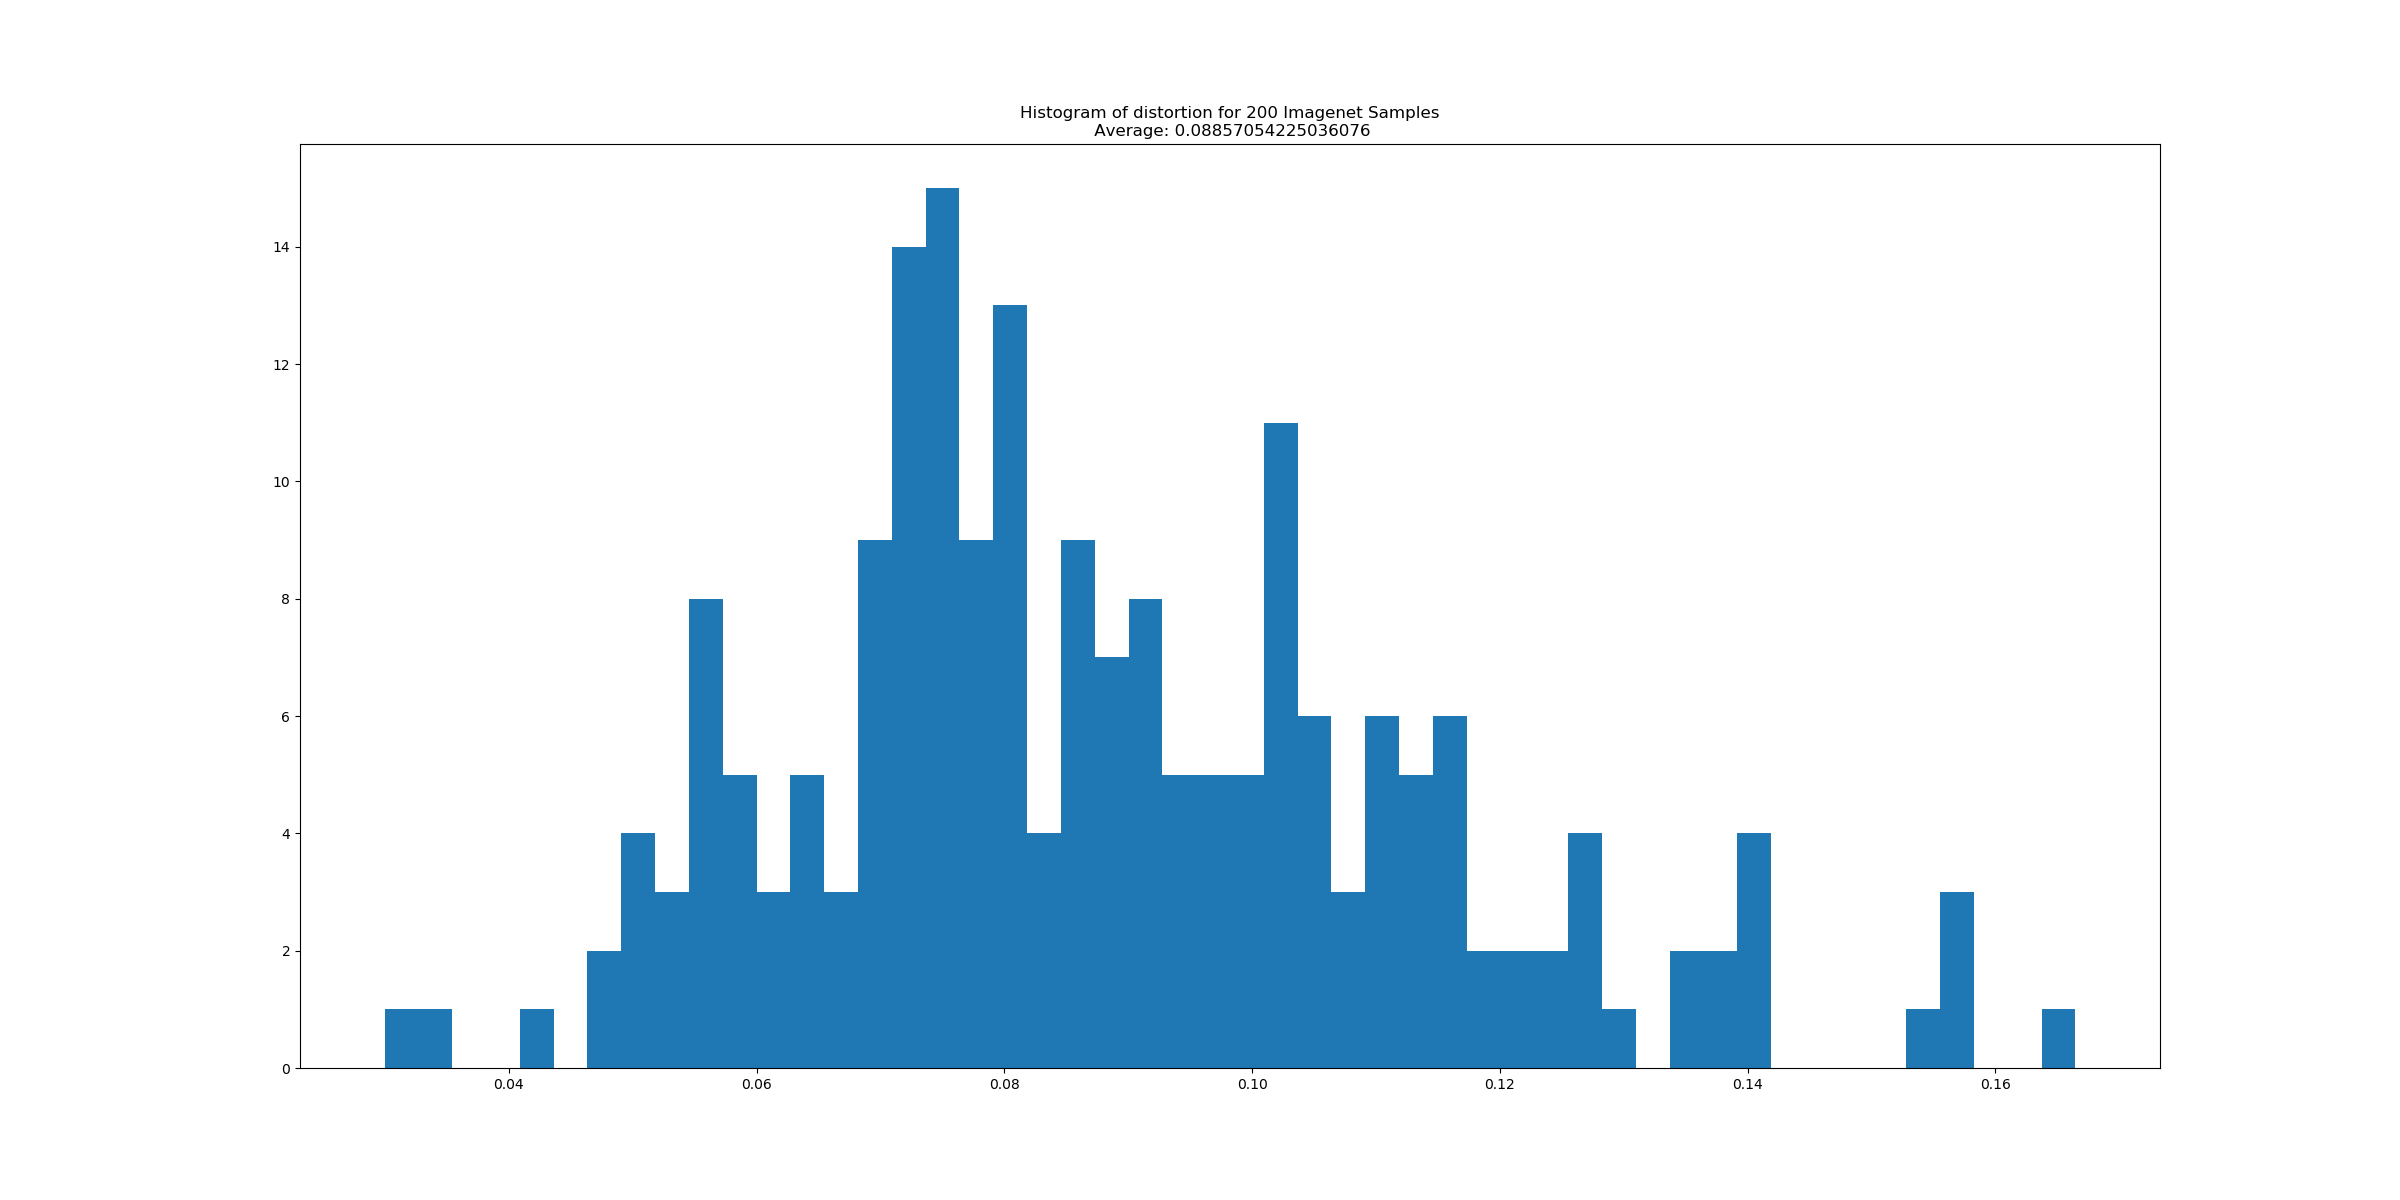
\includegraphics[trim=200 80 100 100, clip,width=7cm]{c3_figures/gamma_sigma/FC200-200-10-distortion_hist.png}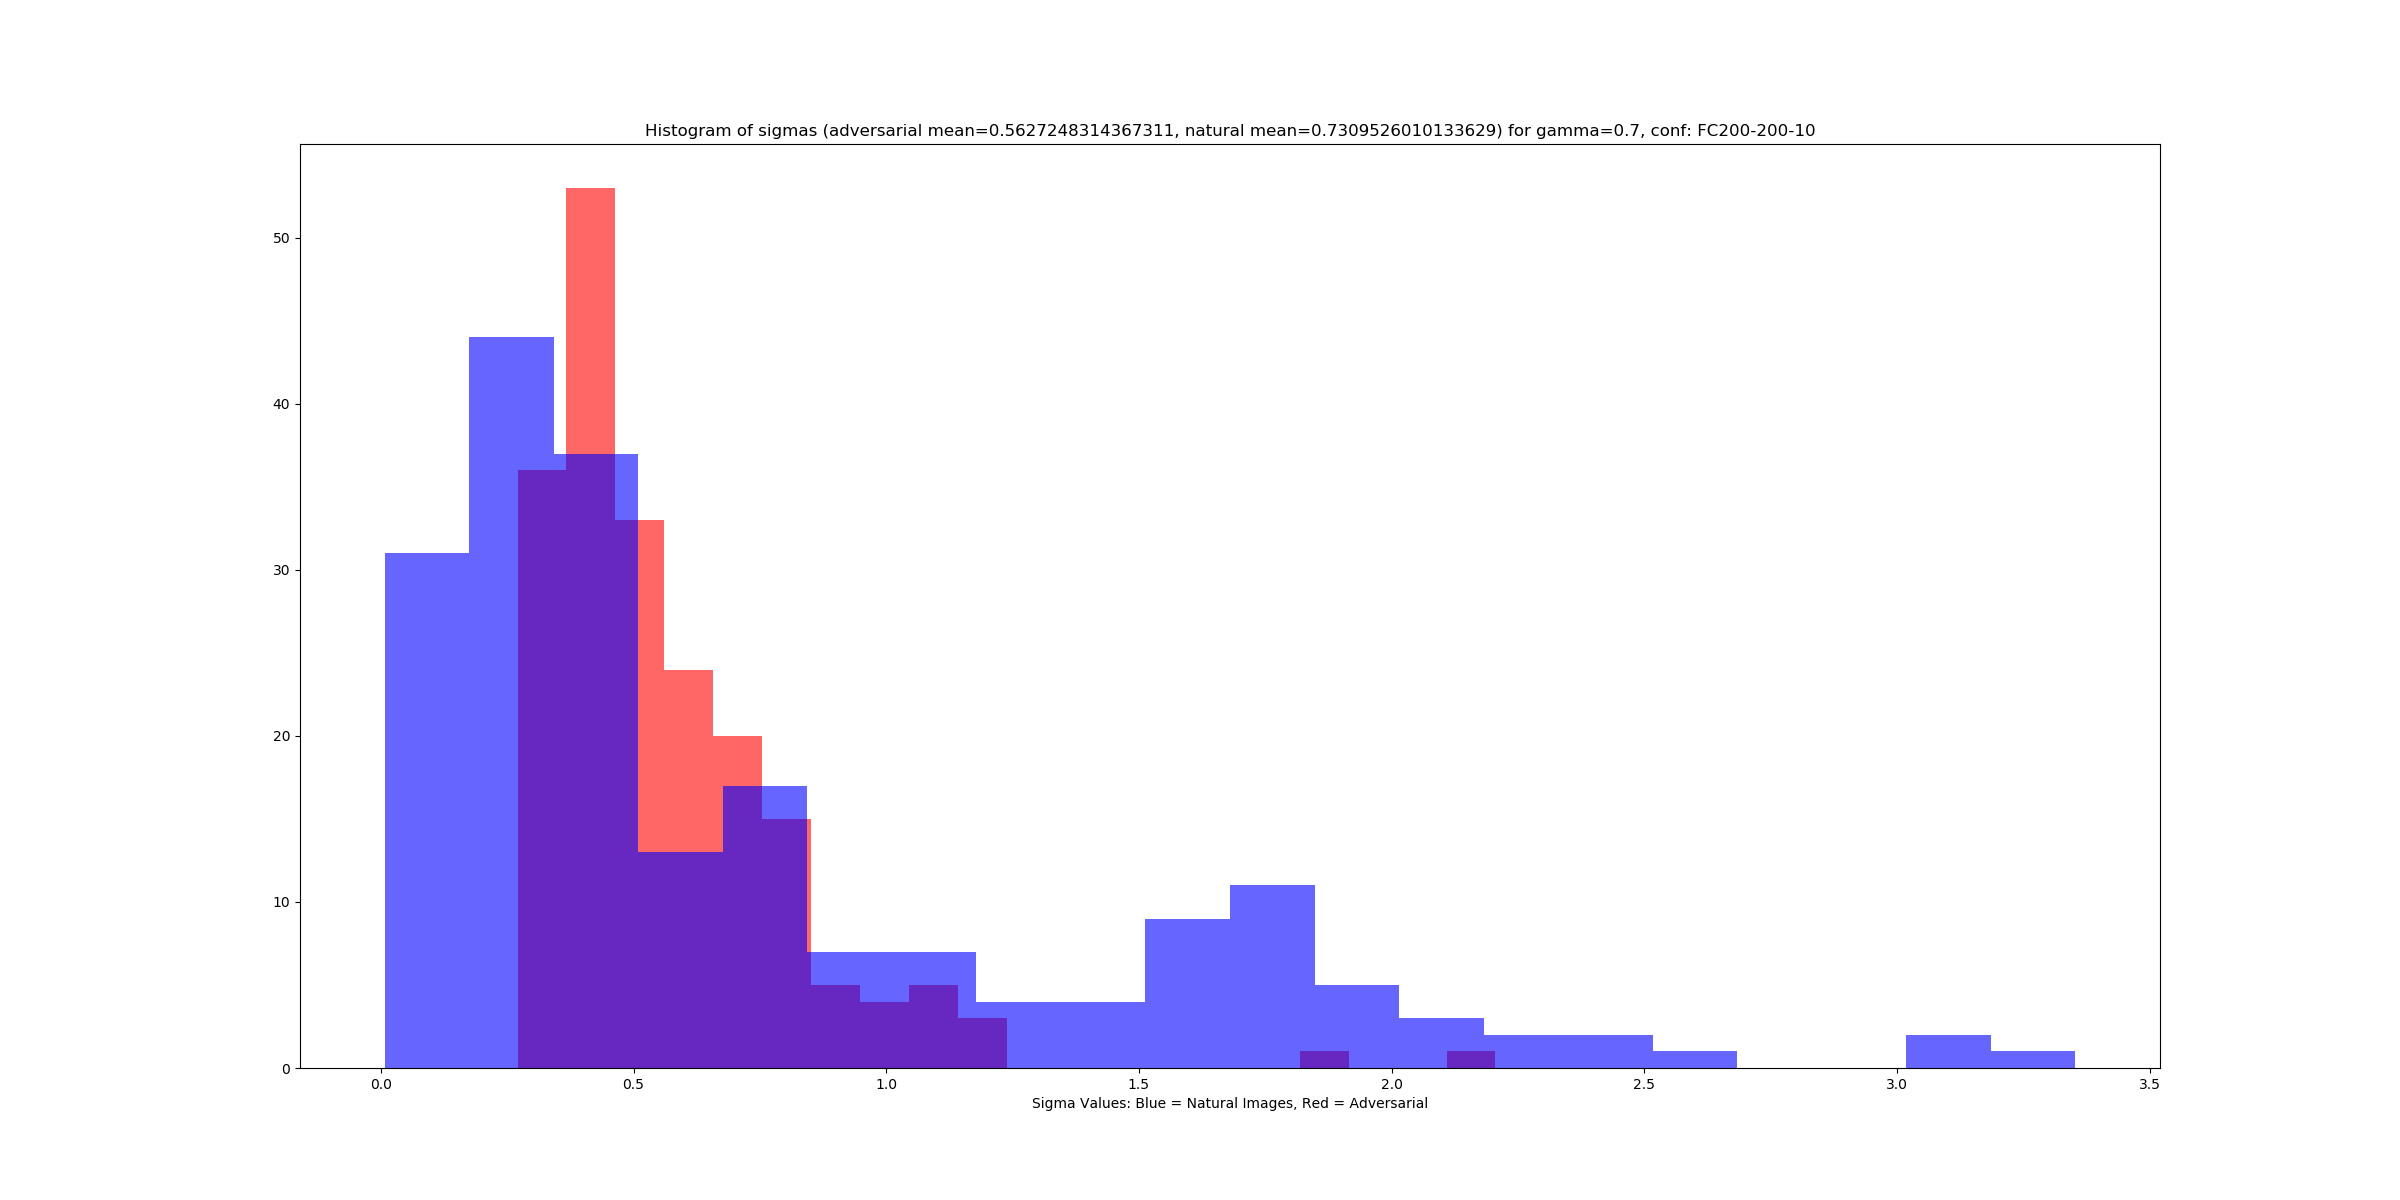
\includegraphics[trim=200 80 100 100, clip,width=7cm]{c3_figures/gamma_sigma/FC200-200-10-gamma1_hist.png}

% \caption{Average distortion for adversarial examples (left) and $0.7$-persistence (right) for FC200-200-10 in Table \ref{table1}}
% \label{fig:FC200-200-10}
% \end{figure}

%B^2 -- we're not using state of the art classifiers... used pre-trained classifiers in order to capture state-of-the-art methods. In particular, we

\subsection{Results on ImageNet}

% For ImageNet, various pretrained networks (vgg16, alexnet, resnet18, densenet161, and squeezenet) were downloaded using torchvision and were attacked with a variety of attack methods %(PGD, FGSM, APGD, CW, ??) 
% using the torchattacks package \cite{kim2021torchattacks}. In all of our tests, we begin with a subset of validation images from the given dataset and generate a collection of adversarial attacks based on those images for each combination of model and attack protocol. 

For ImageNet \citep{Imagenet-old}, we used pre-trained ImageNet classification models, including alexnet \cite{alexnet} and vgg16 \cite{simonyan2014very}.
%, resnet18, squeezenet, and densenet161 \cite{}
We then generated attacks based on the ILSVRC 2015 \citep{ILSVRC15} validation images for each of these networks using a variety of modern attack protocols, including Fast Gradient Sign Method (FGSM \citep{goodfellow_explaining_2014}), Momentum Iterative FGSM (MIFGSM \citep{dongMIFGSM}), Basic Iterative Method (BIM \citep{kurakin_adversarial_2016}), Projected Gradient Descent (PGD \citep{madry_towards_2017}), Randomized FGSM (R+FGSM \citep{tramer2018ensemble}), and Carlini-Wagner (CW ~\cite{carlini_towards_2016}). These were all generated using the TorchAttacks \cite{kim2021torchattacks} toolset.
%We first directly examine neighborhood classification counts as with MNIST and observe a similar dichotomy between original and attacked images. 

\subsubsection{Investigation of $(\gamma, \sigma)$-stability on ImageNet}

In this section, we show the results of Gaussian neighborhood sampling in ImageNet. Figures \ref{fig:imagenet_adv} and \ref{fig:persistent_interpimage} arise from vgg16 and adversarial examples created with BIM; results for other networks and attack strategies are similar, with additional figures in the supplementary material. Figure \ref{fig:imagenet_adv} (left) begins with an image $x$ with label \texttt{goldfinch}. For each equally spaced $\sigma\in(0,2)$, 100 i.i.d. samples were drawn from the Gaussian distribution $N(x,\sigma^2I)$, and the counts of the vgg16 classification for each label are shown. In Figure \ref{fig:imagenet_adv} (right), we see the same plot, but for an adversarial example targeted at the class \texttt{indigo\_bunting}, which is another type of bird, using the BIM attack protocol. %There are similar results with other attack protocols, as described in the supplementary materials.

The key observation in Figure \ref{fig:imagenet_adv} is that the frequency of the class of the adversarial example (\texttt{indigo\_bunting}, shown in red) falls off much quicker than the class for the natural example (\texttt{goldfinch}, shown in black). In this particular example, the original class appears again after the adversarial class becomes less prevalent, but only for a short period of $\sigma$, after which other classes begin to dominate. In some examples the original class does not dominate at all after the decline of the adversarial class. The adversarial class almost never dominates for a long period of $\sigma$. 


% \begin{figure}[ht]
% \centering
% \includegraphics[width = .9\textwidth]
% %[trim=200 80 100 100, clip,width=15cm]
% {./c3_figures/ILSVRC2012_val_00001274-vgg16-sampling.png}
% %\caption{Frequency of each class in Gaussian samples with increasing variance around an adversarial image of a $1$ targeted at $0$ generated using IGSM. The adversarial class is shown as a red curve. The natural image class is shown in black. The bottom shows example sample images.}
% \label{fig:imagenet_natural}
% \caption{Frequency of each class in Gaussian samples with increasing variance around a goldfinch image. Bottom shows example sample images. }
% \end{figure}
%
% \begin{figure}[p]
% \centering
% \includegraphics[width = .9\textwidth]
% {./c3_figures/IMNET-class-11-vgg16-RFGSM-48-attack_data-023.png}
% \end{figure}

\begin{figure}[ht]
\centering
\includegraphics[width = .49\textwidth]
%[trim=200 80 100 100, clip,width=15cm]
{./c3_figures/ILSVRC2012_val_00001274-vgg16-sampling.png}
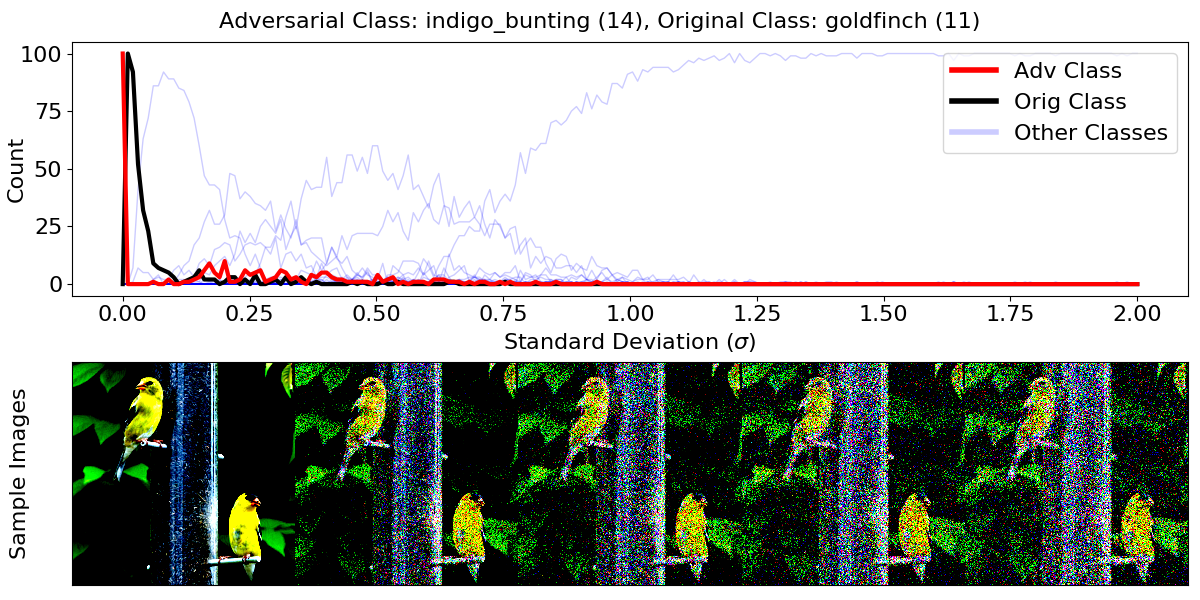
\includegraphics[width = .49\textwidth]
{./c3_figures/IMNET-class-11-vgg16-BIM-48-attack_data-023.png}
%%% Creator: Matplotlib, PGF backend
%%
%% To include the figure in your LaTeX document, write
%%   \input{<filename>.pgf}
%%
%% Make sure the required packages are loaded in your preamble
%%   \usepackage{pgf}
%%
%% and, on pdftex
%%   \usepackage[utf8]{inputenc}\DeclareUnicodeCharacter{2212}{-}
%%
%% or, on luatex and xetex
%%   \usepackage{unicode-math}
%%
%% Figures using additional raster images can only be included by \input if
%% they are in the same directory as the main LaTeX file. For loading figures
%% from other directories you can use the `import` package
%%   \usepackage{import}
%%
%% and then include the figures with
%%   \import{<path to file>}{<filename>.pgf}
%%
%% Matplotlib used the following preamble
%%   \usepackage{fontspec}
%%   \setmainfont{DejaVuSerif.ttf}[Path=C:/Users/glickenstein/anaconda3/lib/site-packages/matplotlib/mpl-data/fonts/ttf/]
%%   \setsansfont{DejaVuSans.ttf}[Path=C:/Users/glickenstein/anaconda3/lib/site-packages/matplotlib/mpl-data/fonts/ttf/]
%%   \setmonofont{DejaVuSansMono.ttf}[Path=C:/Users/glickenstein/anaconda3/lib/site-packages/matplotlib/mpl-data/fonts/ttf/]
%%
\begingroup%
\makeatletter%
\begin{pgfpicture}%
\pgfpathrectangle{\pgfpointorigin}{\pgfqpoint{5.000000in}{2.500000in}}%
\pgfusepath{use as bounding box, clip}%
\begin{pgfscope}%
\pgfsetbuttcap%
\pgfsetmiterjoin%
\definecolor{currentfill}{rgb}{1.000000,1.000000,1.000000}%
\pgfsetfillcolor{currentfill}%
\pgfsetlinewidth{0.000000pt}%
\definecolor{currentstroke}{rgb}{1.000000,1.000000,1.000000}%
\pgfsetstrokecolor{currentstroke}%
\pgfsetdash{}{0pt}%
\pgfpathmoveto{\pgfqpoint{0.000000in}{0.000000in}}%
\pgfpathlineto{\pgfqpoint{5.000000in}{0.000000in}}%
\pgfpathlineto{\pgfqpoint{5.000000in}{2.500000in}}%
\pgfpathlineto{\pgfqpoint{0.000000in}{2.500000in}}%
\pgfpathclose%
\pgfusepath{fill}%
\end{pgfscope}%
\begin{pgfscope}%
\pgfsetbuttcap%
\pgfsetmiterjoin%
\definecolor{currentfill}{rgb}{1.000000,1.000000,1.000000}%
\pgfsetfillcolor{currentfill}%
\pgfsetlinewidth{0.000000pt}%
\definecolor{currentstroke}{rgb}{0.000000,0.000000,0.000000}%
\pgfsetstrokecolor{currentstroke}%
\pgfsetstrokeopacity{0.000000}%
\pgfsetdash{}{0pt}%
\pgfpathmoveto{\pgfqpoint{0.300000in}{1.350000in}}%
\pgfpathlineto{\pgfqpoint{4.950000in}{1.350000in}}%
\pgfpathlineto{\pgfqpoint{4.950000in}{2.475000in}}%
\pgfpathlineto{\pgfqpoint{0.300000in}{2.475000in}}%
\pgfpathclose%
\pgfusepath{fill}%
\end{pgfscope}%
\begin{pgfscope}%
\pgfsetbuttcap%
\pgfsetroundjoin%
\definecolor{currentfill}{rgb}{0.000000,0.000000,0.000000}%
\pgfsetfillcolor{currentfill}%
\pgfsetlinewidth{0.803000pt}%
\definecolor{currentstroke}{rgb}{0.000000,0.000000,0.000000}%
\pgfsetstrokecolor{currentstroke}%
\pgfsetdash{}{0pt}%
\pgfsys@defobject{currentmarker}{\pgfqpoint{0.000000in}{-0.048611in}}{\pgfqpoint{0.000000in}{0.000000in}}{%
\pgfpathmoveto{\pgfqpoint{0.000000in}{0.000000in}}%
\pgfpathlineto{\pgfqpoint{0.000000in}{-0.048611in}}%
\pgfusepath{stroke,fill}%
}%
\begin{pgfscope}%
\pgfsys@transformshift{0.511364in}{1.350000in}%
\pgfsys@useobject{currentmarker}{}%
\end{pgfscope}%
\end{pgfscope}%
\begin{pgfscope}%
\definecolor{textcolor}{rgb}{0.000000,0.000000,0.000000}%
\pgfsetstrokecolor{textcolor}%
\pgfsetfillcolor{textcolor}%
\pgftext[x=0.511364in,y=1.252778in,,top]{\color{textcolor}\sffamily\fontsize{16.000000}{19.200000}\selectfont 0.0}%
\end{pgfscope}%
\begin{pgfscope}%
\pgfsetbuttcap%
\pgfsetroundjoin%
\definecolor{currentfill}{rgb}{0.000000,0.000000,0.000000}%
\pgfsetfillcolor{currentfill}%
\pgfsetlinewidth{0.803000pt}%
\definecolor{currentstroke}{rgb}{0.000000,0.000000,0.000000}%
\pgfsetstrokecolor{currentstroke}%
\pgfsetdash{}{0pt}%
\pgfsys@defobject{currentmarker}{\pgfqpoint{0.000000in}{-0.048611in}}{\pgfqpoint{0.000000in}{0.000000in}}{%
\pgfpathmoveto{\pgfqpoint{0.000000in}{0.000000in}}%
\pgfpathlineto{\pgfqpoint{0.000000in}{-0.048611in}}%
\pgfusepath{stroke,fill}%
}%
\begin{pgfscope}%
\pgfsys@transformshift{1.356818in}{1.350000in}%
\pgfsys@useobject{currentmarker}{}%
\end{pgfscope}%
\end{pgfscope}%
\begin{pgfscope}%
\definecolor{textcolor}{rgb}{0.000000,0.000000,0.000000}%
\pgfsetstrokecolor{textcolor}%
\pgfsetfillcolor{textcolor}%
\pgftext[x=1.356818in,y=1.252778in,,top]{\color{textcolor}\sffamily\fontsize{16.000000}{19.200000}\selectfont 0.2}%
\end{pgfscope}%
\begin{pgfscope}%
\pgfsetbuttcap%
\pgfsetroundjoin%
\definecolor{currentfill}{rgb}{0.000000,0.000000,0.000000}%
\pgfsetfillcolor{currentfill}%
\pgfsetlinewidth{0.803000pt}%
\definecolor{currentstroke}{rgb}{0.000000,0.000000,0.000000}%
\pgfsetstrokecolor{currentstroke}%
\pgfsetdash{}{0pt}%
\pgfsys@defobject{currentmarker}{\pgfqpoint{0.000000in}{-0.048611in}}{\pgfqpoint{0.000000in}{0.000000in}}{%
\pgfpathmoveto{\pgfqpoint{0.000000in}{0.000000in}}%
\pgfpathlineto{\pgfqpoint{0.000000in}{-0.048611in}}%
\pgfusepath{stroke,fill}%
}%
\begin{pgfscope}%
\pgfsys@transformshift{2.202273in}{1.350000in}%
\pgfsys@useobject{currentmarker}{}%
\end{pgfscope}%
\end{pgfscope}%
\begin{pgfscope}%
\definecolor{textcolor}{rgb}{0.000000,0.000000,0.000000}%
\pgfsetstrokecolor{textcolor}%
\pgfsetfillcolor{textcolor}%
\pgftext[x=2.202273in,y=1.252778in,,top]{\color{textcolor}\sffamily\fontsize{16.000000}{19.200000}\selectfont 0.4}%
\end{pgfscope}%
\begin{pgfscope}%
\pgfsetbuttcap%
\pgfsetroundjoin%
\definecolor{currentfill}{rgb}{0.000000,0.000000,0.000000}%
\pgfsetfillcolor{currentfill}%
\pgfsetlinewidth{0.803000pt}%
\definecolor{currentstroke}{rgb}{0.000000,0.000000,0.000000}%
\pgfsetstrokecolor{currentstroke}%
\pgfsetdash{}{0pt}%
\pgfsys@defobject{currentmarker}{\pgfqpoint{0.000000in}{-0.048611in}}{\pgfqpoint{0.000000in}{0.000000in}}{%
\pgfpathmoveto{\pgfqpoint{0.000000in}{0.000000in}}%
\pgfpathlineto{\pgfqpoint{0.000000in}{-0.048611in}}%
\pgfusepath{stroke,fill}%
}%
\begin{pgfscope}%
\pgfsys@transformshift{3.047727in}{1.350000in}%
\pgfsys@useobject{currentmarker}{}%
\end{pgfscope}%
\end{pgfscope}%
\begin{pgfscope}%
\definecolor{textcolor}{rgb}{0.000000,0.000000,0.000000}%
\pgfsetstrokecolor{textcolor}%
\pgfsetfillcolor{textcolor}%
\pgftext[x=3.047727in,y=1.252778in,,top]{\color{textcolor}\sffamily\fontsize{16.000000}{19.200000}\selectfont 0.6}%
\end{pgfscope}%
\begin{pgfscope}%
\pgfsetbuttcap%
\pgfsetroundjoin%
\definecolor{currentfill}{rgb}{0.000000,0.000000,0.000000}%
\pgfsetfillcolor{currentfill}%
\pgfsetlinewidth{0.803000pt}%
\definecolor{currentstroke}{rgb}{0.000000,0.000000,0.000000}%
\pgfsetstrokecolor{currentstroke}%
\pgfsetdash{}{0pt}%
\pgfsys@defobject{currentmarker}{\pgfqpoint{0.000000in}{-0.048611in}}{\pgfqpoint{0.000000in}{0.000000in}}{%
\pgfpathmoveto{\pgfqpoint{0.000000in}{0.000000in}}%
\pgfpathlineto{\pgfqpoint{0.000000in}{-0.048611in}}%
\pgfusepath{stroke,fill}%
}%
\begin{pgfscope}%
\pgfsys@transformshift{3.893182in}{1.350000in}%
\pgfsys@useobject{currentmarker}{}%
\end{pgfscope}%
\end{pgfscope}%
\begin{pgfscope}%
\definecolor{textcolor}{rgb}{0.000000,0.000000,0.000000}%
\pgfsetstrokecolor{textcolor}%
\pgfsetfillcolor{textcolor}%
\pgftext[x=3.893182in,y=1.252778in,,top]{\color{textcolor}\sffamily\fontsize{16.000000}{19.200000}\selectfont 0.8}%
\end{pgfscope}%
\begin{pgfscope}%
\pgfsetbuttcap%
\pgfsetroundjoin%
\definecolor{currentfill}{rgb}{0.000000,0.000000,0.000000}%
\pgfsetfillcolor{currentfill}%
\pgfsetlinewidth{0.803000pt}%
\definecolor{currentstroke}{rgb}{0.000000,0.000000,0.000000}%
\pgfsetstrokecolor{currentstroke}%
\pgfsetdash{}{0pt}%
\pgfsys@defobject{currentmarker}{\pgfqpoint{0.000000in}{-0.048611in}}{\pgfqpoint{0.000000in}{0.000000in}}{%
\pgfpathmoveto{\pgfqpoint{0.000000in}{0.000000in}}%
\pgfpathlineto{\pgfqpoint{0.000000in}{-0.048611in}}%
\pgfusepath{stroke,fill}%
}%
\begin{pgfscope}%
\pgfsys@transformshift{4.738636in}{1.350000in}%
\pgfsys@useobject{currentmarker}{}%
\end{pgfscope}%
\end{pgfscope}%
\begin{pgfscope}%
\definecolor{textcolor}{rgb}{0.000000,0.000000,0.000000}%
\pgfsetstrokecolor{textcolor}%
\pgfsetfillcolor{textcolor}%
\pgftext[x=4.738636in,y=1.252778in,,top]{\color{textcolor}\sffamily\fontsize{16.000000}{19.200000}\selectfont 1.0}%
\end{pgfscope}%
\begin{pgfscope}%
\definecolor{textcolor}{rgb}{0.000000,0.000000,0.000000}%
\pgfsetstrokecolor{textcolor}%
\pgfsetfillcolor{textcolor}%
\pgftext[x=2.625000in,y=0.982162in,,top]{\color{textcolor}\sffamily\fontsize{16.000000}{19.200000}\selectfont Standard Deviation (\(\displaystyle \sigma\))}%
\end{pgfscope}%
\begin{pgfscope}%
\pgfsetbuttcap%
\pgfsetroundjoin%
\definecolor{currentfill}{rgb}{0.000000,0.000000,0.000000}%
\pgfsetfillcolor{currentfill}%
\pgfsetlinewidth{0.803000pt}%
\definecolor{currentstroke}{rgb}{0.000000,0.000000,0.000000}%
\pgfsetstrokecolor{currentstroke}%
\pgfsetdash{}{0pt}%
\pgfsys@defobject{currentmarker}{\pgfqpoint{-0.048611in}{0.000000in}}{\pgfqpoint{0.000000in}{0.000000in}}{%
\pgfpathmoveto{\pgfqpoint{0.000000in}{0.000000in}}%
\pgfpathlineto{\pgfqpoint{-0.048611in}{0.000000in}}%
\pgfusepath{stroke,fill}%
}%
\begin{pgfscope}%
\pgfsys@transformshift{0.300000in}{1.401136in}%
\pgfsys@useobject{currentmarker}{}%
\end{pgfscope}%
\end{pgfscope}%
\begin{pgfscope}%
\definecolor{textcolor}{rgb}{0.000000,0.000000,0.000000}%
\pgfsetstrokecolor{textcolor}%
\pgfsetfillcolor{textcolor}%
\pgftext[x=0.061393in, y=1.316718in, left, base]{\color{textcolor}\sffamily\fontsize{16.000000}{19.200000}\selectfont 0}%
\end{pgfscope}%
\begin{pgfscope}%
\pgfsetbuttcap%
\pgfsetroundjoin%
\definecolor{currentfill}{rgb}{0.000000,0.000000,0.000000}%
\pgfsetfillcolor{currentfill}%
\pgfsetlinewidth{0.803000pt}%
\definecolor{currentstroke}{rgb}{0.000000,0.000000,0.000000}%
\pgfsetstrokecolor{currentstroke}%
\pgfsetdash{}{0pt}%
\pgfsys@defobject{currentmarker}{\pgfqpoint{-0.048611in}{0.000000in}}{\pgfqpoint{0.000000in}{0.000000in}}{%
\pgfpathmoveto{\pgfqpoint{0.000000in}{0.000000in}}%
\pgfpathlineto{\pgfqpoint{-0.048611in}{0.000000in}}%
\pgfusepath{stroke,fill}%
}%
\begin{pgfscope}%
\pgfsys@transformshift{0.300000in}{2.423864in}%
\pgfsys@useobject{currentmarker}{}%
\end{pgfscope}%
\end{pgfscope}%
\begin{pgfscope}%
\definecolor{textcolor}{rgb}{0.000000,0.000000,0.000000}%
\pgfsetstrokecolor{textcolor}%
\pgfsetfillcolor{textcolor}%
\pgftext[x=-0.221376in, y=2.339445in, left, base]{\color{textcolor}\sffamily\fontsize{16.000000}{19.200000}\selectfont 100}%
\end{pgfscope}%
\begin{pgfscope}%
\definecolor{textcolor}{rgb}{0.000000,0.000000,0.000000}%
\pgfsetstrokecolor{textcolor}%
\pgfsetfillcolor{textcolor}%
\pgftext[x=-0.151931in,y=1.912500in,,bottom,rotate=90.000000]{\color{textcolor}\sffamily\fontsize{16.000000}{19.200000}\selectfont Count}%
\end{pgfscope}%
\begin{pgfscope}%
\pgfpathrectangle{\pgfqpoint{0.300000in}{1.350000in}}{\pgfqpoint{4.650000in}{1.125000in}}%
\pgfusepath{clip}%
\pgfsetrectcap%
\pgfsetroundjoin%
\pgfsetlinewidth{1.003750pt}%
\definecolor{currentstroke}{rgb}{0.000000,0.000000,1.000000}%
\pgfsetstrokecolor{currentstroke}%
\pgfsetstrokeopacity{0.200000}%
\pgfsetdash{}{0pt}%
\pgfpathmoveto{\pgfqpoint{0.511364in}{1.401136in}}%
\pgfpathlineto{\pgfqpoint{2.848047in}{1.401136in}}%
\pgfpathlineto{\pgfqpoint{2.869290in}{1.411364in}}%
\pgfpathlineto{\pgfqpoint{2.890532in}{1.401136in}}%
\pgfpathlineto{\pgfqpoint{2.954260in}{1.401136in}}%
\pgfpathlineto{\pgfqpoint{2.996745in}{1.421591in}}%
\pgfpathlineto{\pgfqpoint{3.017988in}{1.401136in}}%
\pgfpathlineto{\pgfqpoint{3.039230in}{1.401136in}}%
\pgfpathlineto{\pgfqpoint{3.060473in}{1.411364in}}%
\pgfpathlineto{\pgfqpoint{3.081715in}{1.401136in}}%
\pgfpathlineto{\pgfqpoint{3.102958in}{1.401136in}}%
\pgfpathlineto{\pgfqpoint{3.124201in}{1.411364in}}%
\pgfpathlineto{\pgfqpoint{3.145443in}{1.401136in}}%
\pgfpathlineto{\pgfqpoint{3.357869in}{1.401136in}}%
\pgfpathlineto{\pgfqpoint{3.379111in}{1.421591in}}%
\pgfpathlineto{\pgfqpoint{3.400354in}{1.401136in}}%
\pgfpathlineto{\pgfqpoint{3.506567in}{1.401136in}}%
\pgfpathlineto{\pgfqpoint{3.527810in}{1.411364in}}%
\pgfpathlineto{\pgfqpoint{3.549052in}{1.401136in}}%
\pgfpathlineto{\pgfqpoint{3.634022in}{1.401136in}}%
\pgfpathlineto{\pgfqpoint{3.655265in}{1.411364in}}%
\pgfpathlineto{\pgfqpoint{3.676508in}{1.401136in}}%
\pgfpathlineto{\pgfqpoint{3.697750in}{1.431818in}}%
\pgfpathlineto{\pgfqpoint{3.761478in}{1.401136in}}%
\pgfpathlineto{\pgfqpoint{3.782720in}{1.431818in}}%
\pgfpathlineto{\pgfqpoint{3.803963in}{1.401136in}}%
\pgfpathlineto{\pgfqpoint{3.825206in}{1.401136in}}%
\pgfpathlineto{\pgfqpoint{3.846448in}{1.411364in}}%
\pgfpathlineto{\pgfqpoint{3.867691in}{1.401136in}}%
\pgfpathlineto{\pgfqpoint{3.888933in}{1.411364in}}%
\pgfpathlineto{\pgfqpoint{3.910176in}{1.401136in}}%
\pgfpathlineto{\pgfqpoint{3.931418in}{1.411364in}}%
\pgfpathlineto{\pgfqpoint{3.952661in}{1.401136in}}%
\pgfpathlineto{\pgfqpoint{3.973904in}{1.421591in}}%
\pgfpathlineto{\pgfqpoint{3.995146in}{1.421591in}}%
\pgfpathlineto{\pgfqpoint{4.016389in}{1.411364in}}%
\pgfpathlineto{\pgfqpoint{4.037631in}{1.411364in}}%
\pgfpathlineto{\pgfqpoint{4.058874in}{1.401136in}}%
\pgfpathlineto{\pgfqpoint{4.080116in}{1.411364in}}%
\pgfpathlineto{\pgfqpoint{4.101359in}{1.401136in}}%
\pgfpathlineto{\pgfqpoint{4.122602in}{1.411364in}}%
\pgfpathlineto{\pgfqpoint{4.143844in}{1.431818in}}%
\pgfpathlineto{\pgfqpoint{4.165087in}{1.421591in}}%
\pgfpathlineto{\pgfqpoint{4.186329in}{1.421591in}}%
\pgfpathlineto{\pgfqpoint{4.207572in}{1.401136in}}%
\pgfpathlineto{\pgfqpoint{4.228815in}{1.401136in}}%
\pgfpathlineto{\pgfqpoint{4.250057in}{1.421591in}}%
\pgfpathlineto{\pgfqpoint{4.271300in}{1.421591in}}%
\pgfpathlineto{\pgfqpoint{4.292542in}{1.401136in}}%
\pgfpathlineto{\pgfqpoint{4.313785in}{1.411364in}}%
\pgfpathlineto{\pgfqpoint{4.335027in}{1.411364in}}%
\pgfpathlineto{\pgfqpoint{4.356270in}{1.421591in}}%
\pgfpathlineto{\pgfqpoint{4.377513in}{1.411364in}}%
\pgfpathlineto{\pgfqpoint{4.398755in}{1.421591in}}%
\pgfpathlineto{\pgfqpoint{4.419998in}{1.411364in}}%
\pgfpathlineto{\pgfqpoint{4.441240in}{1.411364in}}%
\pgfpathlineto{\pgfqpoint{4.462483in}{1.442045in}}%
\pgfpathlineto{\pgfqpoint{4.483725in}{1.421591in}}%
\pgfpathlineto{\pgfqpoint{4.504968in}{1.442045in}}%
\pgfpathlineto{\pgfqpoint{4.526211in}{1.401136in}}%
\pgfpathlineto{\pgfqpoint{4.547453in}{1.401136in}}%
\pgfpathlineto{\pgfqpoint{4.568696in}{1.431818in}}%
\pgfpathlineto{\pgfqpoint{4.589938in}{1.421591in}}%
\pgfpathlineto{\pgfqpoint{4.611181in}{1.421591in}}%
\pgfpathlineto{\pgfqpoint{4.632423in}{1.401136in}}%
\pgfpathlineto{\pgfqpoint{4.674909in}{1.442045in}}%
\pgfpathlineto{\pgfqpoint{4.696151in}{1.421591in}}%
\pgfpathlineto{\pgfqpoint{4.717394in}{1.421591in}}%
\pgfpathlineto{\pgfqpoint{4.738636in}{1.431818in}}%
\pgfpathlineto{\pgfqpoint{4.738636in}{1.431818in}}%
\pgfusepath{stroke}%
\end{pgfscope}%
\begin{pgfscope}%
\pgfpathrectangle{\pgfqpoint{0.300000in}{1.350000in}}{\pgfqpoint{4.650000in}{1.125000in}}%
\pgfusepath{clip}%
\pgfsetrectcap%
\pgfsetroundjoin%
\pgfsetlinewidth{1.003750pt}%
\definecolor{currentstroke}{rgb}{0.000000,0.000000,1.000000}%
\pgfsetstrokecolor{currentstroke}%
\pgfsetstrokeopacity{0.200000}%
\pgfsetdash{}{0pt}%
\pgfpathmoveto{\pgfqpoint{0.511364in}{1.401136in}}%
\pgfpathlineto{\pgfqpoint{3.187928in}{1.401136in}}%
\pgfpathlineto{\pgfqpoint{3.209171in}{1.411364in}}%
\pgfpathlineto{\pgfqpoint{3.230413in}{1.401136in}}%
\pgfpathlineto{\pgfqpoint{4.165087in}{1.401136in}}%
\pgfpathlineto{\pgfqpoint{4.186329in}{1.411364in}}%
\pgfpathlineto{\pgfqpoint{4.207572in}{1.401136in}}%
\pgfpathlineto{\pgfqpoint{4.377513in}{1.401136in}}%
\pgfpathlineto{\pgfqpoint{4.398755in}{1.411364in}}%
\pgfpathlineto{\pgfqpoint{4.419998in}{1.401136in}}%
\pgfpathlineto{\pgfqpoint{4.738636in}{1.401136in}}%
\pgfpathlineto{\pgfqpoint{4.738636in}{1.401136in}}%
\pgfusepath{stroke}%
\end{pgfscope}%
\begin{pgfscope}%
\pgfpathrectangle{\pgfqpoint{0.300000in}{1.350000in}}{\pgfqpoint{4.650000in}{1.125000in}}%
\pgfusepath{clip}%
\pgfsetrectcap%
\pgfsetroundjoin%
\pgfsetlinewidth{1.003750pt}%
\definecolor{currentstroke}{rgb}{0.000000,0.000000,1.000000}%
\pgfsetstrokecolor{currentstroke}%
\pgfsetstrokeopacity{0.200000}%
\pgfsetdash{}{0pt}%
\pgfpathmoveto{\pgfqpoint{0.511364in}{1.401136in}}%
\pgfpathlineto{\pgfqpoint{0.638819in}{1.401136in}}%
\pgfpathlineto{\pgfqpoint{0.660062in}{1.462500in}}%
\pgfpathlineto{\pgfqpoint{0.681304in}{1.503409in}}%
\pgfpathlineto{\pgfqpoint{0.702547in}{1.667045in}}%
\pgfpathlineto{\pgfqpoint{0.723789in}{1.769318in}}%
\pgfpathlineto{\pgfqpoint{0.766275in}{1.912500in}}%
\pgfpathlineto{\pgfqpoint{0.787517in}{1.973864in}}%
\pgfpathlineto{\pgfqpoint{0.808760in}{2.055682in}}%
\pgfpathlineto{\pgfqpoint{0.830002in}{2.004545in}}%
\pgfpathlineto{\pgfqpoint{0.851245in}{2.086364in}}%
\pgfpathlineto{\pgfqpoint{0.872487in}{2.076136in}}%
\pgfpathlineto{\pgfqpoint{0.893730in}{2.106818in}}%
\pgfpathlineto{\pgfqpoint{0.914973in}{2.076136in}}%
\pgfpathlineto{\pgfqpoint{0.936215in}{2.127273in}}%
\pgfpathlineto{\pgfqpoint{0.957458in}{2.076136in}}%
\pgfpathlineto{\pgfqpoint{0.978700in}{2.127273in}}%
\pgfpathlineto{\pgfqpoint{0.999943in}{2.106818in}}%
\pgfpathlineto{\pgfqpoint{1.021185in}{2.168182in}}%
\pgfpathlineto{\pgfqpoint{1.042428in}{2.250000in}}%
\pgfpathlineto{\pgfqpoint{1.063671in}{2.137500in}}%
\pgfpathlineto{\pgfqpoint{1.084913in}{2.096591in}}%
\pgfpathlineto{\pgfqpoint{1.106156in}{2.147727in}}%
\pgfpathlineto{\pgfqpoint{1.127398in}{2.147727in}}%
\pgfpathlineto{\pgfqpoint{1.148641in}{2.045455in}}%
\pgfpathlineto{\pgfqpoint{1.169884in}{2.219318in}}%
\pgfpathlineto{\pgfqpoint{1.191126in}{2.127273in}}%
\pgfpathlineto{\pgfqpoint{1.212369in}{2.168182in}}%
\pgfpathlineto{\pgfqpoint{1.233611in}{2.168182in}}%
\pgfpathlineto{\pgfqpoint{1.254854in}{2.127273in}}%
\pgfpathlineto{\pgfqpoint{1.276096in}{2.096591in}}%
\pgfpathlineto{\pgfqpoint{1.297339in}{2.035227in}}%
\pgfpathlineto{\pgfqpoint{1.318582in}{2.127273in}}%
\pgfpathlineto{\pgfqpoint{1.339824in}{2.076136in}}%
\pgfpathlineto{\pgfqpoint{1.361067in}{2.086364in}}%
\pgfpathlineto{\pgfqpoint{1.382309in}{2.035227in}}%
\pgfpathlineto{\pgfqpoint{1.403552in}{1.922727in}}%
\pgfpathlineto{\pgfqpoint{1.424794in}{1.892045in}}%
\pgfpathlineto{\pgfqpoint{1.446037in}{1.932955in}}%
\pgfpathlineto{\pgfqpoint{1.467280in}{2.014773in}}%
\pgfpathlineto{\pgfqpoint{1.488522in}{1.820455in}}%
\pgfpathlineto{\pgfqpoint{1.509765in}{1.861364in}}%
\pgfpathlineto{\pgfqpoint{1.531007in}{1.892045in}}%
\pgfpathlineto{\pgfqpoint{1.552250in}{1.789773in}}%
\pgfpathlineto{\pgfqpoint{1.573492in}{1.810227in}}%
\pgfpathlineto{\pgfqpoint{1.594735in}{1.779545in}}%
\pgfpathlineto{\pgfqpoint{1.615978in}{1.759091in}}%
\pgfpathlineto{\pgfqpoint{1.637220in}{1.707955in}}%
\pgfpathlineto{\pgfqpoint{1.658463in}{1.759091in}}%
\pgfpathlineto{\pgfqpoint{1.679705in}{1.738636in}}%
\pgfpathlineto{\pgfqpoint{1.700948in}{1.881818in}}%
\pgfpathlineto{\pgfqpoint{1.722190in}{1.738636in}}%
\pgfpathlineto{\pgfqpoint{1.743433in}{1.789773in}}%
\pgfpathlineto{\pgfqpoint{1.764676in}{1.738636in}}%
\pgfpathlineto{\pgfqpoint{1.785918in}{1.636364in}}%
\pgfpathlineto{\pgfqpoint{1.807161in}{1.626136in}}%
\pgfpathlineto{\pgfqpoint{1.849646in}{1.687500in}}%
\pgfpathlineto{\pgfqpoint{1.870889in}{1.707955in}}%
\pgfpathlineto{\pgfqpoint{1.892131in}{1.687500in}}%
\pgfpathlineto{\pgfqpoint{1.913374in}{1.677273in}}%
\pgfpathlineto{\pgfqpoint{1.934616in}{1.677273in}}%
\pgfpathlineto{\pgfqpoint{1.955859in}{1.667045in}}%
\pgfpathlineto{\pgfqpoint{1.977101in}{1.605682in}}%
\pgfpathlineto{\pgfqpoint{1.998344in}{1.646591in}}%
\pgfpathlineto{\pgfqpoint{2.019587in}{1.605682in}}%
\pgfpathlineto{\pgfqpoint{2.040829in}{1.636364in}}%
\pgfpathlineto{\pgfqpoint{2.062072in}{1.615909in}}%
\pgfpathlineto{\pgfqpoint{2.083314in}{1.605682in}}%
\pgfpathlineto{\pgfqpoint{2.104557in}{1.656818in}}%
\pgfpathlineto{\pgfqpoint{2.125799in}{1.595455in}}%
\pgfpathlineto{\pgfqpoint{2.147042in}{1.646591in}}%
\pgfpathlineto{\pgfqpoint{2.168285in}{1.564773in}}%
\pgfpathlineto{\pgfqpoint{2.189527in}{1.615909in}}%
\pgfpathlineto{\pgfqpoint{2.210770in}{1.544318in}}%
\pgfpathlineto{\pgfqpoint{2.232012in}{1.523864in}}%
\pgfpathlineto{\pgfqpoint{2.253255in}{1.605682in}}%
\pgfpathlineto{\pgfqpoint{2.274497in}{1.544318in}}%
\pgfpathlineto{\pgfqpoint{2.295740in}{1.585227in}}%
\pgfpathlineto{\pgfqpoint{2.316983in}{1.615909in}}%
\pgfpathlineto{\pgfqpoint{2.338225in}{1.605682in}}%
\pgfpathlineto{\pgfqpoint{2.359468in}{1.646591in}}%
\pgfpathlineto{\pgfqpoint{2.380710in}{1.615909in}}%
\pgfpathlineto{\pgfqpoint{2.401953in}{1.595455in}}%
\pgfpathlineto{\pgfqpoint{2.423196in}{1.554545in}}%
\pgfpathlineto{\pgfqpoint{2.444438in}{1.595455in}}%
\pgfpathlineto{\pgfqpoint{2.465681in}{1.523864in}}%
\pgfpathlineto{\pgfqpoint{2.486923in}{1.482955in}}%
\pgfpathlineto{\pgfqpoint{2.508166in}{1.554545in}}%
\pgfpathlineto{\pgfqpoint{2.529408in}{1.534091in}}%
\pgfpathlineto{\pgfqpoint{2.550651in}{1.595455in}}%
\pgfpathlineto{\pgfqpoint{2.571894in}{1.554545in}}%
\pgfpathlineto{\pgfqpoint{2.593136in}{1.482955in}}%
\pgfpathlineto{\pgfqpoint{2.614379in}{1.513636in}}%
\pgfpathlineto{\pgfqpoint{2.635621in}{1.554545in}}%
\pgfpathlineto{\pgfqpoint{2.656864in}{1.482955in}}%
\pgfpathlineto{\pgfqpoint{2.678106in}{1.595455in}}%
\pgfpathlineto{\pgfqpoint{2.699349in}{1.503409in}}%
\pgfpathlineto{\pgfqpoint{2.720592in}{1.503409in}}%
\pgfpathlineto{\pgfqpoint{2.741834in}{1.513636in}}%
\pgfpathlineto{\pgfqpoint{2.763077in}{1.544318in}}%
\pgfpathlineto{\pgfqpoint{2.784319in}{1.544318in}}%
\pgfpathlineto{\pgfqpoint{2.805562in}{1.513636in}}%
\pgfpathlineto{\pgfqpoint{2.826804in}{1.513636in}}%
\pgfpathlineto{\pgfqpoint{2.848047in}{1.472727in}}%
\pgfpathlineto{\pgfqpoint{2.869290in}{1.503409in}}%
\pgfpathlineto{\pgfqpoint{2.890532in}{1.544318in}}%
\pgfpathlineto{\pgfqpoint{2.911775in}{1.503409in}}%
\pgfpathlineto{\pgfqpoint{2.933017in}{1.513636in}}%
\pgfpathlineto{\pgfqpoint{2.954260in}{1.452273in}}%
\pgfpathlineto{\pgfqpoint{2.996745in}{1.472727in}}%
\pgfpathlineto{\pgfqpoint{3.017988in}{1.503409in}}%
\pgfpathlineto{\pgfqpoint{3.039230in}{1.462500in}}%
\pgfpathlineto{\pgfqpoint{3.060473in}{1.523864in}}%
\pgfpathlineto{\pgfqpoint{3.081715in}{1.462500in}}%
\pgfpathlineto{\pgfqpoint{3.102958in}{1.534091in}}%
\pgfpathlineto{\pgfqpoint{3.124201in}{1.482955in}}%
\pgfpathlineto{\pgfqpoint{3.145443in}{1.482955in}}%
\pgfpathlineto{\pgfqpoint{3.166686in}{1.472727in}}%
\pgfpathlineto{\pgfqpoint{3.187928in}{1.482955in}}%
\pgfpathlineto{\pgfqpoint{3.209171in}{1.503409in}}%
\pgfpathlineto{\pgfqpoint{3.230413in}{1.462500in}}%
\pgfpathlineto{\pgfqpoint{3.251656in}{1.442045in}}%
\pgfpathlineto{\pgfqpoint{3.272899in}{1.482955in}}%
\pgfpathlineto{\pgfqpoint{3.294141in}{1.462500in}}%
\pgfpathlineto{\pgfqpoint{3.315384in}{1.493182in}}%
\pgfpathlineto{\pgfqpoint{3.336626in}{1.462500in}}%
\pgfpathlineto{\pgfqpoint{3.357869in}{1.462500in}}%
\pgfpathlineto{\pgfqpoint{3.379111in}{1.431818in}}%
\pgfpathlineto{\pgfqpoint{3.400354in}{1.421591in}}%
\pgfpathlineto{\pgfqpoint{3.421597in}{1.462500in}}%
\pgfpathlineto{\pgfqpoint{3.442839in}{1.472727in}}%
\pgfpathlineto{\pgfqpoint{3.464082in}{1.442045in}}%
\pgfpathlineto{\pgfqpoint{3.485324in}{1.462500in}}%
\pgfpathlineto{\pgfqpoint{3.506567in}{1.452273in}}%
\pgfpathlineto{\pgfqpoint{3.527810in}{1.421591in}}%
\pgfpathlineto{\pgfqpoint{3.549052in}{1.431818in}}%
\pgfpathlineto{\pgfqpoint{3.570295in}{1.462500in}}%
\pgfpathlineto{\pgfqpoint{3.591537in}{1.431818in}}%
\pgfpathlineto{\pgfqpoint{3.612780in}{1.411364in}}%
\pgfpathlineto{\pgfqpoint{3.634022in}{1.452273in}}%
\pgfpathlineto{\pgfqpoint{3.655265in}{1.442045in}}%
\pgfpathlineto{\pgfqpoint{3.676508in}{1.472727in}}%
\pgfpathlineto{\pgfqpoint{3.697750in}{1.452273in}}%
\pgfpathlineto{\pgfqpoint{3.718993in}{1.421591in}}%
\pgfpathlineto{\pgfqpoint{3.740235in}{1.411364in}}%
\pgfpathlineto{\pgfqpoint{3.761478in}{1.442045in}}%
\pgfpathlineto{\pgfqpoint{3.782720in}{1.452273in}}%
\pgfpathlineto{\pgfqpoint{3.803963in}{1.421591in}}%
\pgfpathlineto{\pgfqpoint{3.825206in}{1.401136in}}%
\pgfpathlineto{\pgfqpoint{3.846448in}{1.411364in}}%
\pgfpathlineto{\pgfqpoint{3.867691in}{1.431818in}}%
\pgfpathlineto{\pgfqpoint{3.888933in}{1.411364in}}%
\pgfpathlineto{\pgfqpoint{3.910176in}{1.442045in}}%
\pgfpathlineto{\pgfqpoint{3.931418in}{1.421591in}}%
\pgfpathlineto{\pgfqpoint{3.952661in}{1.442045in}}%
\pgfpathlineto{\pgfqpoint{3.973904in}{1.411364in}}%
\pgfpathlineto{\pgfqpoint{3.995146in}{1.421591in}}%
\pgfpathlineto{\pgfqpoint{4.016389in}{1.442045in}}%
\pgfpathlineto{\pgfqpoint{4.058874in}{1.421591in}}%
\pgfpathlineto{\pgfqpoint{4.080116in}{1.431818in}}%
\pgfpathlineto{\pgfqpoint{4.101359in}{1.421591in}}%
\pgfpathlineto{\pgfqpoint{4.122602in}{1.421591in}}%
\pgfpathlineto{\pgfqpoint{4.143844in}{1.431818in}}%
\pgfpathlineto{\pgfqpoint{4.165087in}{1.411364in}}%
\pgfpathlineto{\pgfqpoint{4.186329in}{1.421591in}}%
\pgfpathlineto{\pgfqpoint{4.207572in}{1.401136in}}%
\pgfpathlineto{\pgfqpoint{4.228815in}{1.411364in}}%
\pgfpathlineto{\pgfqpoint{4.250057in}{1.431818in}}%
\pgfpathlineto{\pgfqpoint{4.271300in}{1.401136in}}%
\pgfpathlineto{\pgfqpoint{4.292542in}{1.411364in}}%
\pgfpathlineto{\pgfqpoint{4.313785in}{1.401136in}}%
\pgfpathlineto{\pgfqpoint{4.335027in}{1.411364in}}%
\pgfpathlineto{\pgfqpoint{4.356270in}{1.401136in}}%
\pgfpathlineto{\pgfqpoint{4.377513in}{1.411364in}}%
\pgfpathlineto{\pgfqpoint{4.398755in}{1.411364in}}%
\pgfpathlineto{\pgfqpoint{4.419998in}{1.421591in}}%
\pgfpathlineto{\pgfqpoint{4.441240in}{1.401136in}}%
\pgfpathlineto{\pgfqpoint{4.504968in}{1.401136in}}%
\pgfpathlineto{\pgfqpoint{4.526211in}{1.411364in}}%
\pgfpathlineto{\pgfqpoint{4.547453in}{1.411364in}}%
\pgfpathlineto{\pgfqpoint{4.568696in}{1.401136in}}%
\pgfpathlineto{\pgfqpoint{4.589938in}{1.401136in}}%
\pgfpathlineto{\pgfqpoint{4.611181in}{1.411364in}}%
\pgfpathlineto{\pgfqpoint{4.632423in}{1.401136in}}%
\pgfpathlineto{\pgfqpoint{4.717394in}{1.401136in}}%
\pgfpathlineto{\pgfqpoint{4.738636in}{1.411364in}}%
\pgfpathlineto{\pgfqpoint{4.738636in}{1.411364in}}%
\pgfusepath{stroke}%
\end{pgfscope}%
\begin{pgfscope}%
\pgfpathrectangle{\pgfqpoint{0.300000in}{1.350000in}}{\pgfqpoint{4.650000in}{1.125000in}}%
\pgfusepath{clip}%
\pgfsetrectcap%
\pgfsetroundjoin%
\pgfsetlinewidth{1.003750pt}%
\definecolor{currentstroke}{rgb}{0.000000,0.000000,1.000000}%
\pgfsetstrokecolor{currentstroke}%
\pgfsetstrokeopacity{0.200000}%
\pgfsetdash{}{0pt}%
\pgfpathmoveto{\pgfqpoint{0.511364in}{1.401136in}}%
\pgfpathlineto{\pgfqpoint{0.575091in}{1.401136in}}%
\pgfpathlineto{\pgfqpoint{0.596334in}{1.431818in}}%
\pgfpathlineto{\pgfqpoint{0.617577in}{1.452273in}}%
\pgfpathlineto{\pgfqpoint{0.638819in}{1.513636in}}%
\pgfpathlineto{\pgfqpoint{0.660062in}{1.513636in}}%
\pgfpathlineto{\pgfqpoint{0.681304in}{1.503409in}}%
\pgfpathlineto{\pgfqpoint{0.702547in}{1.503409in}}%
\pgfpathlineto{\pgfqpoint{0.723789in}{1.472727in}}%
\pgfpathlineto{\pgfqpoint{0.745032in}{1.421591in}}%
\pgfpathlineto{\pgfqpoint{0.766275in}{1.411364in}}%
\pgfpathlineto{\pgfqpoint{0.787517in}{1.411364in}}%
\pgfpathlineto{\pgfqpoint{0.808760in}{1.421591in}}%
\pgfpathlineto{\pgfqpoint{0.851245in}{1.401136in}}%
\pgfpathlineto{\pgfqpoint{0.914973in}{1.401136in}}%
\pgfpathlineto{\pgfqpoint{0.936215in}{1.411364in}}%
\pgfpathlineto{\pgfqpoint{0.957458in}{1.401136in}}%
\pgfpathlineto{\pgfqpoint{0.978700in}{1.411364in}}%
\pgfpathlineto{\pgfqpoint{0.999943in}{1.411364in}}%
\pgfpathlineto{\pgfqpoint{1.021185in}{1.401136in}}%
\pgfpathlineto{\pgfqpoint{1.127398in}{1.401136in}}%
\pgfpathlineto{\pgfqpoint{1.148641in}{1.411364in}}%
\pgfpathlineto{\pgfqpoint{1.169884in}{1.401136in}}%
\pgfpathlineto{\pgfqpoint{4.738636in}{1.401136in}}%
\pgfpathlineto{\pgfqpoint{4.738636in}{1.401136in}}%
\pgfusepath{stroke}%
\end{pgfscope}%
\begin{pgfscope}%
\pgfpathrectangle{\pgfqpoint{0.300000in}{1.350000in}}{\pgfqpoint{4.650000in}{1.125000in}}%
\pgfusepath{clip}%
\pgfsetrectcap%
\pgfsetroundjoin%
\pgfsetlinewidth{1.003750pt}%
\definecolor{currentstroke}{rgb}{0.000000,0.000000,1.000000}%
\pgfsetstrokecolor{currentstroke}%
\pgfsetstrokeopacity{0.200000}%
\pgfsetdash{}{0pt}%
\pgfpathmoveto{\pgfqpoint{0.511364in}{1.401136in}}%
\pgfpathlineto{\pgfqpoint{0.553849in}{1.401136in}}%
\pgfpathlineto{\pgfqpoint{0.575091in}{1.442045in}}%
\pgfpathlineto{\pgfqpoint{0.596334in}{1.442045in}}%
\pgfpathlineto{\pgfqpoint{0.617577in}{1.421591in}}%
\pgfpathlineto{\pgfqpoint{0.638819in}{1.544318in}}%
\pgfpathlineto{\pgfqpoint{0.660062in}{1.554545in}}%
\pgfpathlineto{\pgfqpoint{0.681304in}{1.544318in}}%
\pgfpathlineto{\pgfqpoint{0.702547in}{1.442045in}}%
\pgfpathlineto{\pgfqpoint{0.723789in}{1.411364in}}%
\pgfpathlineto{\pgfqpoint{0.745032in}{1.421591in}}%
\pgfpathlineto{\pgfqpoint{0.766275in}{1.401136in}}%
\pgfpathlineto{\pgfqpoint{4.738636in}{1.401136in}}%
\pgfpathlineto{\pgfqpoint{4.738636in}{1.401136in}}%
\pgfusepath{stroke}%
\end{pgfscope}%
\begin{pgfscope}%
\pgfpathrectangle{\pgfqpoint{0.300000in}{1.350000in}}{\pgfqpoint{4.650000in}{1.125000in}}%
\pgfusepath{clip}%
\pgfsetrectcap%
\pgfsetroundjoin%
\pgfsetlinewidth{1.003750pt}%
\definecolor{currentstroke}{rgb}{0.000000,0.000000,1.000000}%
\pgfsetstrokecolor{currentstroke}%
\pgfsetstrokeopacity{0.200000}%
\pgfsetdash{}{0pt}%
\pgfpathmoveto{\pgfqpoint{0.511364in}{1.401136in}}%
\pgfpathlineto{\pgfqpoint{2.040829in}{1.401136in}}%
\pgfpathlineto{\pgfqpoint{2.062072in}{1.411364in}}%
\pgfpathlineto{\pgfqpoint{2.083314in}{1.401136in}}%
\pgfpathlineto{\pgfqpoint{2.189527in}{1.401136in}}%
\pgfpathlineto{\pgfqpoint{2.210770in}{1.411364in}}%
\pgfpathlineto{\pgfqpoint{2.232012in}{1.401136in}}%
\pgfpathlineto{\pgfqpoint{2.253255in}{1.401136in}}%
\pgfpathlineto{\pgfqpoint{2.274497in}{1.411364in}}%
\pgfpathlineto{\pgfqpoint{2.295740in}{1.401136in}}%
\pgfpathlineto{\pgfqpoint{2.316983in}{1.401136in}}%
\pgfpathlineto{\pgfqpoint{2.338225in}{1.431818in}}%
\pgfpathlineto{\pgfqpoint{2.359468in}{1.411364in}}%
\pgfpathlineto{\pgfqpoint{2.380710in}{1.401136in}}%
\pgfpathlineto{\pgfqpoint{2.423196in}{1.401136in}}%
\pgfpathlineto{\pgfqpoint{2.444438in}{1.411364in}}%
\pgfpathlineto{\pgfqpoint{2.465681in}{1.401136in}}%
\pgfpathlineto{\pgfqpoint{2.486923in}{1.431818in}}%
\pgfpathlineto{\pgfqpoint{2.508166in}{1.411364in}}%
\pgfpathlineto{\pgfqpoint{2.571894in}{1.442045in}}%
\pgfpathlineto{\pgfqpoint{2.593136in}{1.401136in}}%
\pgfpathlineto{\pgfqpoint{2.614379in}{1.401136in}}%
\pgfpathlineto{\pgfqpoint{2.635621in}{1.442045in}}%
\pgfpathlineto{\pgfqpoint{2.656864in}{1.411364in}}%
\pgfpathlineto{\pgfqpoint{2.678106in}{1.431818in}}%
\pgfpathlineto{\pgfqpoint{2.699349in}{1.431818in}}%
\pgfpathlineto{\pgfqpoint{2.741834in}{1.452273in}}%
\pgfpathlineto{\pgfqpoint{2.763077in}{1.411364in}}%
\pgfpathlineto{\pgfqpoint{2.784319in}{1.421591in}}%
\pgfpathlineto{\pgfqpoint{2.826804in}{1.421591in}}%
\pgfpathlineto{\pgfqpoint{2.848047in}{1.452273in}}%
\pgfpathlineto{\pgfqpoint{2.869290in}{1.462500in}}%
\pgfpathlineto{\pgfqpoint{2.890532in}{1.452273in}}%
\pgfpathlineto{\pgfqpoint{2.911775in}{1.411364in}}%
\pgfpathlineto{\pgfqpoint{2.933017in}{1.431818in}}%
\pgfpathlineto{\pgfqpoint{2.954260in}{1.442045in}}%
\pgfpathlineto{\pgfqpoint{2.975503in}{1.482955in}}%
\pgfpathlineto{\pgfqpoint{2.996745in}{1.452273in}}%
\pgfpathlineto{\pgfqpoint{3.017988in}{1.442045in}}%
\pgfpathlineto{\pgfqpoint{3.039230in}{1.411364in}}%
\pgfpathlineto{\pgfqpoint{3.060473in}{1.462500in}}%
\pgfpathlineto{\pgfqpoint{3.081715in}{1.462500in}}%
\pgfpathlineto{\pgfqpoint{3.102958in}{1.431818in}}%
\pgfpathlineto{\pgfqpoint{3.124201in}{1.442045in}}%
\pgfpathlineto{\pgfqpoint{3.145443in}{1.493182in}}%
\pgfpathlineto{\pgfqpoint{3.166686in}{1.442045in}}%
\pgfpathlineto{\pgfqpoint{3.187928in}{1.493182in}}%
\pgfpathlineto{\pgfqpoint{3.209171in}{1.431818in}}%
\pgfpathlineto{\pgfqpoint{3.230413in}{1.411364in}}%
\pgfpathlineto{\pgfqpoint{3.251656in}{1.431818in}}%
\pgfpathlineto{\pgfqpoint{3.272899in}{1.442045in}}%
\pgfpathlineto{\pgfqpoint{3.294141in}{1.472727in}}%
\pgfpathlineto{\pgfqpoint{3.315384in}{1.421591in}}%
\pgfpathlineto{\pgfqpoint{3.336626in}{1.421591in}}%
\pgfpathlineto{\pgfqpoint{3.357869in}{1.462500in}}%
\pgfpathlineto{\pgfqpoint{3.379111in}{1.421591in}}%
\pgfpathlineto{\pgfqpoint{3.400354in}{1.442045in}}%
\pgfpathlineto{\pgfqpoint{3.421597in}{1.472727in}}%
\pgfpathlineto{\pgfqpoint{3.442839in}{1.431818in}}%
\pgfpathlineto{\pgfqpoint{3.464082in}{1.472727in}}%
\pgfpathlineto{\pgfqpoint{3.485324in}{1.452273in}}%
\pgfpathlineto{\pgfqpoint{3.506567in}{1.421591in}}%
\pgfpathlineto{\pgfqpoint{3.527810in}{1.431818in}}%
\pgfpathlineto{\pgfqpoint{3.549052in}{1.472727in}}%
\pgfpathlineto{\pgfqpoint{3.570295in}{1.442045in}}%
\pgfpathlineto{\pgfqpoint{3.591537in}{1.452273in}}%
\pgfpathlineto{\pgfqpoint{3.612780in}{1.431818in}}%
\pgfpathlineto{\pgfqpoint{3.634022in}{1.462500in}}%
\pgfpathlineto{\pgfqpoint{3.655265in}{1.411364in}}%
\pgfpathlineto{\pgfqpoint{3.676508in}{1.431818in}}%
\pgfpathlineto{\pgfqpoint{3.697750in}{1.421591in}}%
\pgfpathlineto{\pgfqpoint{3.718993in}{1.472727in}}%
\pgfpathlineto{\pgfqpoint{3.740235in}{1.503409in}}%
\pgfpathlineto{\pgfqpoint{3.761478in}{1.421591in}}%
\pgfpathlineto{\pgfqpoint{3.782720in}{1.421591in}}%
\pgfpathlineto{\pgfqpoint{3.803963in}{1.411364in}}%
\pgfpathlineto{\pgfqpoint{3.825206in}{1.442045in}}%
\pgfpathlineto{\pgfqpoint{3.888933in}{1.411364in}}%
\pgfpathlineto{\pgfqpoint{3.910176in}{1.411364in}}%
\pgfpathlineto{\pgfqpoint{3.931418in}{1.421591in}}%
\pgfpathlineto{\pgfqpoint{3.952661in}{1.411364in}}%
\pgfpathlineto{\pgfqpoint{3.973904in}{1.411364in}}%
\pgfpathlineto{\pgfqpoint{3.995146in}{1.442045in}}%
\pgfpathlineto{\pgfqpoint{4.016389in}{1.421591in}}%
\pgfpathlineto{\pgfqpoint{4.037631in}{1.421591in}}%
\pgfpathlineto{\pgfqpoint{4.058874in}{1.411364in}}%
\pgfpathlineto{\pgfqpoint{4.080116in}{1.421591in}}%
\pgfpathlineto{\pgfqpoint{4.101359in}{1.411364in}}%
\pgfpathlineto{\pgfqpoint{4.122602in}{1.411364in}}%
\pgfpathlineto{\pgfqpoint{4.143844in}{1.442045in}}%
\pgfpathlineto{\pgfqpoint{4.186329in}{1.421591in}}%
\pgfpathlineto{\pgfqpoint{4.207572in}{1.421591in}}%
\pgfpathlineto{\pgfqpoint{4.228815in}{1.431818in}}%
\pgfpathlineto{\pgfqpoint{4.250057in}{1.401136in}}%
\pgfpathlineto{\pgfqpoint{4.271300in}{1.431818in}}%
\pgfpathlineto{\pgfqpoint{4.292542in}{1.401136in}}%
\pgfpathlineto{\pgfqpoint{4.335027in}{1.421591in}}%
\pgfpathlineto{\pgfqpoint{4.356270in}{1.421591in}}%
\pgfpathlineto{\pgfqpoint{4.377513in}{1.401136in}}%
\pgfpathlineto{\pgfqpoint{4.398755in}{1.411364in}}%
\pgfpathlineto{\pgfqpoint{4.419998in}{1.401136in}}%
\pgfpathlineto{\pgfqpoint{4.441240in}{1.401136in}}%
\pgfpathlineto{\pgfqpoint{4.462483in}{1.411364in}}%
\pgfpathlineto{\pgfqpoint{4.483725in}{1.411364in}}%
\pgfpathlineto{\pgfqpoint{4.504968in}{1.401136in}}%
\pgfpathlineto{\pgfqpoint{4.526211in}{1.411364in}}%
\pgfpathlineto{\pgfqpoint{4.547453in}{1.401136in}}%
\pgfpathlineto{\pgfqpoint{4.589938in}{1.401136in}}%
\pgfpathlineto{\pgfqpoint{4.611181in}{1.411364in}}%
\pgfpathlineto{\pgfqpoint{4.632423in}{1.401136in}}%
\pgfpathlineto{\pgfqpoint{4.653666in}{1.411364in}}%
\pgfpathlineto{\pgfqpoint{4.674909in}{1.411364in}}%
\pgfpathlineto{\pgfqpoint{4.696151in}{1.431818in}}%
\pgfpathlineto{\pgfqpoint{4.717394in}{1.401136in}}%
\pgfpathlineto{\pgfqpoint{4.738636in}{1.401136in}}%
\pgfpathlineto{\pgfqpoint{4.738636in}{1.401136in}}%
\pgfusepath{stroke}%
\end{pgfscope}%
\begin{pgfscope}%
\pgfpathrectangle{\pgfqpoint{0.300000in}{1.350000in}}{\pgfqpoint{4.650000in}{1.125000in}}%
\pgfusepath{clip}%
\pgfsetrectcap%
\pgfsetroundjoin%
\pgfsetlinewidth{1.003750pt}%
\definecolor{currentstroke}{rgb}{0.000000,0.000000,1.000000}%
\pgfsetstrokecolor{currentstroke}%
\pgfsetstrokeopacity{0.200000}%
\pgfsetdash{}{0pt}%
\pgfpathmoveto{\pgfqpoint{0.511364in}{1.401136in}}%
\pgfpathlineto{\pgfqpoint{1.021185in}{1.401136in}}%
\pgfpathlineto{\pgfqpoint{1.042428in}{1.411364in}}%
\pgfpathlineto{\pgfqpoint{1.063671in}{1.411364in}}%
\pgfpathlineto{\pgfqpoint{1.084913in}{1.421591in}}%
\pgfpathlineto{\pgfqpoint{1.127398in}{1.401136in}}%
\pgfpathlineto{\pgfqpoint{1.148641in}{1.421591in}}%
\pgfpathlineto{\pgfqpoint{1.191126in}{1.421591in}}%
\pgfpathlineto{\pgfqpoint{1.212369in}{1.431818in}}%
\pgfpathlineto{\pgfqpoint{1.254854in}{1.411364in}}%
\pgfpathlineto{\pgfqpoint{1.297339in}{1.452273in}}%
\pgfpathlineto{\pgfqpoint{1.318582in}{1.421591in}}%
\pgfpathlineto{\pgfqpoint{1.339824in}{1.431818in}}%
\pgfpathlineto{\pgfqpoint{1.361067in}{1.411364in}}%
\pgfpathlineto{\pgfqpoint{1.382309in}{1.421591in}}%
\pgfpathlineto{\pgfqpoint{1.403552in}{1.442045in}}%
\pgfpathlineto{\pgfqpoint{1.424794in}{1.401136in}}%
\pgfpathlineto{\pgfqpoint{1.446037in}{1.401136in}}%
\pgfpathlineto{\pgfqpoint{1.467280in}{1.421591in}}%
\pgfpathlineto{\pgfqpoint{1.488522in}{1.421591in}}%
\pgfpathlineto{\pgfqpoint{1.509765in}{1.411364in}}%
\pgfpathlineto{\pgfqpoint{1.531007in}{1.411364in}}%
\pgfpathlineto{\pgfqpoint{1.573492in}{1.431818in}}%
\pgfpathlineto{\pgfqpoint{1.594735in}{1.421591in}}%
\pgfpathlineto{\pgfqpoint{1.637220in}{1.442045in}}%
\pgfpathlineto{\pgfqpoint{1.658463in}{1.411364in}}%
\pgfpathlineto{\pgfqpoint{1.679705in}{1.401136in}}%
\pgfpathlineto{\pgfqpoint{1.700948in}{1.421591in}}%
\pgfpathlineto{\pgfqpoint{1.722190in}{1.431818in}}%
\pgfpathlineto{\pgfqpoint{1.743433in}{1.421591in}}%
\pgfpathlineto{\pgfqpoint{1.764676in}{1.401136in}}%
\pgfpathlineto{\pgfqpoint{1.785918in}{1.411364in}}%
\pgfpathlineto{\pgfqpoint{1.807161in}{1.401136in}}%
\pgfpathlineto{\pgfqpoint{1.828403in}{1.411364in}}%
\pgfpathlineto{\pgfqpoint{1.892131in}{1.411364in}}%
\pgfpathlineto{\pgfqpoint{1.913374in}{1.401136in}}%
\pgfpathlineto{\pgfqpoint{1.934616in}{1.411364in}}%
\pgfpathlineto{\pgfqpoint{1.955859in}{1.401136in}}%
\pgfpathlineto{\pgfqpoint{2.125799in}{1.401136in}}%
\pgfpathlineto{\pgfqpoint{2.147042in}{1.411364in}}%
\pgfpathlineto{\pgfqpoint{2.168285in}{1.401136in}}%
\pgfpathlineto{\pgfqpoint{2.189527in}{1.401136in}}%
\pgfpathlineto{\pgfqpoint{2.210770in}{1.411364in}}%
\pgfpathlineto{\pgfqpoint{2.232012in}{1.401136in}}%
\pgfpathlineto{\pgfqpoint{2.338225in}{1.401136in}}%
\pgfpathlineto{\pgfqpoint{2.359468in}{1.411364in}}%
\pgfpathlineto{\pgfqpoint{2.380710in}{1.401136in}}%
\pgfpathlineto{\pgfqpoint{2.401953in}{1.411364in}}%
\pgfpathlineto{\pgfqpoint{2.423196in}{1.411364in}}%
\pgfpathlineto{\pgfqpoint{2.444438in}{1.401136in}}%
\pgfpathlineto{\pgfqpoint{2.465681in}{1.401136in}}%
\pgfpathlineto{\pgfqpoint{2.486923in}{1.411364in}}%
\pgfpathlineto{\pgfqpoint{2.508166in}{1.401136in}}%
\pgfpathlineto{\pgfqpoint{2.529408in}{1.411364in}}%
\pgfpathlineto{\pgfqpoint{2.550651in}{1.411364in}}%
\pgfpathlineto{\pgfqpoint{2.571894in}{1.401136in}}%
\pgfpathlineto{\pgfqpoint{2.614379in}{1.401136in}}%
\pgfpathlineto{\pgfqpoint{2.635621in}{1.411364in}}%
\pgfpathlineto{\pgfqpoint{2.656864in}{1.401136in}}%
\pgfpathlineto{\pgfqpoint{4.738636in}{1.401136in}}%
\pgfpathlineto{\pgfqpoint{4.738636in}{1.401136in}}%
\pgfusepath{stroke}%
\end{pgfscope}%
\begin{pgfscope}%
\pgfpathrectangle{\pgfqpoint{0.300000in}{1.350000in}}{\pgfqpoint{4.650000in}{1.125000in}}%
\pgfusepath{clip}%
\pgfsetrectcap%
\pgfsetroundjoin%
\pgfsetlinewidth{1.003750pt}%
\definecolor{currentstroke}{rgb}{0.000000,0.000000,1.000000}%
\pgfsetstrokecolor{currentstroke}%
\pgfsetstrokeopacity{0.200000}%
\pgfsetdash{}{0pt}%
\pgfpathmoveto{\pgfqpoint{0.511364in}{1.401136in}}%
\pgfpathlineto{\pgfqpoint{3.421597in}{1.401136in}}%
\pgfpathlineto{\pgfqpoint{3.442839in}{1.411364in}}%
\pgfpathlineto{\pgfqpoint{3.464082in}{1.401136in}}%
\pgfpathlineto{\pgfqpoint{3.867691in}{1.401136in}}%
\pgfpathlineto{\pgfqpoint{3.888933in}{1.411364in}}%
\pgfpathlineto{\pgfqpoint{3.910176in}{1.411364in}}%
\pgfpathlineto{\pgfqpoint{3.931418in}{1.401136in}}%
\pgfpathlineto{\pgfqpoint{4.738636in}{1.401136in}}%
\pgfpathlineto{\pgfqpoint{4.738636in}{1.401136in}}%
\pgfusepath{stroke}%
\end{pgfscope}%
\begin{pgfscope}%
\pgfpathrectangle{\pgfqpoint{0.300000in}{1.350000in}}{\pgfqpoint{4.650000in}{1.125000in}}%
\pgfusepath{clip}%
\pgfsetrectcap%
\pgfsetroundjoin%
\pgfsetlinewidth{1.003750pt}%
\definecolor{currentstroke}{rgb}{0.000000,0.000000,1.000000}%
\pgfsetstrokecolor{currentstroke}%
\pgfsetstrokeopacity{0.200000}%
\pgfsetdash{}{0pt}%
\pgfpathmoveto{\pgfqpoint{0.511364in}{1.401136in}}%
\pgfpathlineto{\pgfqpoint{0.745032in}{1.401136in}}%
\pgfpathlineto{\pgfqpoint{0.766275in}{1.411364in}}%
\pgfpathlineto{\pgfqpoint{0.787517in}{1.401136in}}%
\pgfpathlineto{\pgfqpoint{0.914973in}{1.401136in}}%
\pgfpathlineto{\pgfqpoint{0.936215in}{1.411364in}}%
\pgfpathlineto{\pgfqpoint{0.957458in}{1.411364in}}%
\pgfpathlineto{\pgfqpoint{0.978700in}{1.401136in}}%
\pgfpathlineto{\pgfqpoint{0.999943in}{1.401136in}}%
\pgfpathlineto{\pgfqpoint{1.021185in}{1.431818in}}%
\pgfpathlineto{\pgfqpoint{1.042428in}{1.401136in}}%
\pgfpathlineto{\pgfqpoint{1.084913in}{1.401136in}}%
\pgfpathlineto{\pgfqpoint{1.106156in}{1.411364in}}%
\pgfpathlineto{\pgfqpoint{1.148641in}{1.411364in}}%
\pgfpathlineto{\pgfqpoint{1.169884in}{1.401136in}}%
\pgfpathlineto{\pgfqpoint{1.212369in}{1.401136in}}%
\pgfpathlineto{\pgfqpoint{1.233611in}{1.411364in}}%
\pgfpathlineto{\pgfqpoint{1.254854in}{1.401136in}}%
\pgfpathlineto{\pgfqpoint{1.276096in}{1.401136in}}%
\pgfpathlineto{\pgfqpoint{1.297339in}{1.411364in}}%
\pgfpathlineto{\pgfqpoint{1.318582in}{1.401136in}}%
\pgfpathlineto{\pgfqpoint{1.339824in}{1.401136in}}%
\pgfpathlineto{\pgfqpoint{1.361067in}{1.421591in}}%
\pgfpathlineto{\pgfqpoint{1.382309in}{1.401136in}}%
\pgfpathlineto{\pgfqpoint{1.424794in}{1.401136in}}%
\pgfpathlineto{\pgfqpoint{1.446037in}{1.411364in}}%
\pgfpathlineto{\pgfqpoint{1.488522in}{1.411364in}}%
\pgfpathlineto{\pgfqpoint{1.509765in}{1.401136in}}%
\pgfpathlineto{\pgfqpoint{4.738636in}{1.401136in}}%
\pgfpathlineto{\pgfqpoint{4.738636in}{1.401136in}}%
\pgfusepath{stroke}%
\end{pgfscope}%
\begin{pgfscope}%
\pgfpathrectangle{\pgfqpoint{0.300000in}{1.350000in}}{\pgfqpoint{4.650000in}{1.125000in}}%
\pgfusepath{clip}%
\pgfsetrectcap%
\pgfsetroundjoin%
\pgfsetlinewidth{1.003750pt}%
\definecolor{currentstroke}{rgb}{0.000000,0.000000,1.000000}%
\pgfsetstrokecolor{currentstroke}%
\pgfsetstrokeopacity{0.200000}%
\pgfsetdash{}{0pt}%
\pgfpathmoveto{\pgfqpoint{0.511364in}{1.401136in}}%
\pgfpathlineto{\pgfqpoint{3.910176in}{1.401136in}}%
\pgfpathlineto{\pgfqpoint{3.931418in}{1.411364in}}%
\pgfpathlineto{\pgfqpoint{3.952661in}{1.401136in}}%
\pgfpathlineto{\pgfqpoint{4.738636in}{1.401136in}}%
\pgfpathlineto{\pgfqpoint{4.738636in}{1.401136in}}%
\pgfusepath{stroke}%
\end{pgfscope}%
\begin{pgfscope}%
\pgfpathrectangle{\pgfqpoint{0.300000in}{1.350000in}}{\pgfqpoint{4.650000in}{1.125000in}}%
\pgfusepath{clip}%
\pgfsetrectcap%
\pgfsetroundjoin%
\pgfsetlinewidth{1.003750pt}%
\definecolor{currentstroke}{rgb}{0.000000,0.000000,1.000000}%
\pgfsetstrokecolor{currentstroke}%
\pgfsetstrokeopacity{0.200000}%
\pgfsetdash{}{0pt}%
\pgfpathmoveto{\pgfqpoint{0.511364in}{2.423864in}}%
\pgfpathlineto{\pgfqpoint{0.553849in}{2.423864in}}%
\pgfpathlineto{\pgfqpoint{0.575091in}{2.311364in}}%
\pgfpathlineto{\pgfqpoint{0.596334in}{2.229545in}}%
\pgfpathlineto{\pgfqpoint{0.617577in}{2.168182in}}%
\pgfpathlineto{\pgfqpoint{0.660062in}{1.748864in}}%
\pgfpathlineto{\pgfqpoint{0.681304in}{1.636364in}}%
\pgfpathlineto{\pgfqpoint{0.702547in}{1.513636in}}%
\pgfpathlineto{\pgfqpoint{0.723789in}{1.421591in}}%
\pgfpathlineto{\pgfqpoint{0.745032in}{1.401136in}}%
\pgfpathlineto{\pgfqpoint{0.766275in}{1.411364in}}%
\pgfpathlineto{\pgfqpoint{0.787517in}{1.411364in}}%
\pgfpathlineto{\pgfqpoint{0.808760in}{1.401136in}}%
\pgfpathlineto{\pgfqpoint{4.738636in}{1.401136in}}%
\pgfpathlineto{\pgfqpoint{4.738636in}{1.401136in}}%
\pgfusepath{stroke}%
\end{pgfscope}%
\begin{pgfscope}%
\pgfpathrectangle{\pgfqpoint{0.300000in}{1.350000in}}{\pgfqpoint{4.650000in}{1.125000in}}%
\pgfusepath{clip}%
\pgfsetrectcap%
\pgfsetroundjoin%
\pgfsetlinewidth{1.003750pt}%
\definecolor{currentstroke}{rgb}{0.000000,0.000000,1.000000}%
\pgfsetstrokecolor{currentstroke}%
\pgfsetstrokeopacity{0.200000}%
\pgfsetdash{}{0pt}%
\pgfpathmoveto{\pgfqpoint{0.511364in}{1.401136in}}%
\pgfpathlineto{\pgfqpoint{3.294141in}{1.401136in}}%
\pgfpathlineto{\pgfqpoint{3.315384in}{1.411364in}}%
\pgfpathlineto{\pgfqpoint{3.336626in}{1.401136in}}%
\pgfpathlineto{\pgfqpoint{4.738636in}{1.401136in}}%
\pgfpathlineto{\pgfqpoint{4.738636in}{1.401136in}}%
\pgfusepath{stroke}%
\end{pgfscope}%
\begin{pgfscope}%
\pgfpathrectangle{\pgfqpoint{0.300000in}{1.350000in}}{\pgfqpoint{4.650000in}{1.125000in}}%
\pgfusepath{clip}%
\pgfsetrectcap%
\pgfsetroundjoin%
\pgfsetlinewidth{1.003750pt}%
\definecolor{currentstroke}{rgb}{0.000000,0.000000,1.000000}%
\pgfsetstrokecolor{currentstroke}%
\pgfsetstrokeopacity{0.200000}%
\pgfsetdash{}{0pt}%
\pgfpathmoveto{\pgfqpoint{0.511364in}{1.401136in}}%
\pgfpathlineto{\pgfqpoint{2.911775in}{1.401136in}}%
\pgfpathlineto{\pgfqpoint{2.933017in}{1.411364in}}%
\pgfpathlineto{\pgfqpoint{2.954260in}{1.401136in}}%
\pgfpathlineto{\pgfqpoint{2.996745in}{1.421591in}}%
\pgfpathlineto{\pgfqpoint{3.017988in}{1.401136in}}%
\pgfpathlineto{\pgfqpoint{3.060473in}{1.401136in}}%
\pgfpathlineto{\pgfqpoint{3.081715in}{1.431818in}}%
\pgfpathlineto{\pgfqpoint{3.102958in}{1.411364in}}%
\pgfpathlineto{\pgfqpoint{3.124201in}{1.401136in}}%
\pgfpathlineto{\pgfqpoint{3.145443in}{1.401136in}}%
\pgfpathlineto{\pgfqpoint{3.166686in}{1.411364in}}%
\pgfpathlineto{\pgfqpoint{3.187928in}{1.411364in}}%
\pgfpathlineto{\pgfqpoint{3.209171in}{1.431818in}}%
\pgfpathlineto{\pgfqpoint{3.230413in}{1.442045in}}%
\pgfpathlineto{\pgfqpoint{3.251656in}{1.431818in}}%
\pgfpathlineto{\pgfqpoint{3.272899in}{1.431818in}}%
\pgfpathlineto{\pgfqpoint{3.294141in}{1.401136in}}%
\pgfpathlineto{\pgfqpoint{3.315384in}{1.421591in}}%
\pgfpathlineto{\pgfqpoint{3.336626in}{1.421591in}}%
\pgfpathlineto{\pgfqpoint{3.357869in}{1.431818in}}%
\pgfpathlineto{\pgfqpoint{3.379111in}{1.452273in}}%
\pgfpathlineto{\pgfqpoint{3.400354in}{1.462500in}}%
\pgfpathlineto{\pgfqpoint{3.421597in}{1.431818in}}%
\pgfpathlineto{\pgfqpoint{3.442839in}{1.431818in}}%
\pgfpathlineto{\pgfqpoint{3.464082in}{1.462500in}}%
\pgfpathlineto{\pgfqpoint{3.485324in}{1.442045in}}%
\pgfpathlineto{\pgfqpoint{3.506567in}{1.472727in}}%
\pgfpathlineto{\pgfqpoint{3.527810in}{1.472727in}}%
\pgfpathlineto{\pgfqpoint{3.549052in}{1.442045in}}%
\pgfpathlineto{\pgfqpoint{3.591537in}{1.503409in}}%
\pgfpathlineto{\pgfqpoint{3.612780in}{1.472727in}}%
\pgfpathlineto{\pgfqpoint{3.634022in}{1.482955in}}%
\pgfpathlineto{\pgfqpoint{3.655265in}{1.534091in}}%
\pgfpathlineto{\pgfqpoint{3.676508in}{1.472727in}}%
\pgfpathlineto{\pgfqpoint{3.697750in}{1.534091in}}%
\pgfpathlineto{\pgfqpoint{3.718993in}{1.513636in}}%
\pgfpathlineto{\pgfqpoint{3.740235in}{1.523864in}}%
\pgfpathlineto{\pgfqpoint{3.761478in}{1.564773in}}%
\pgfpathlineto{\pgfqpoint{3.782720in}{1.554545in}}%
\pgfpathlineto{\pgfqpoint{3.825206in}{1.615909in}}%
\pgfpathlineto{\pgfqpoint{3.846448in}{1.564773in}}%
\pgfpathlineto{\pgfqpoint{3.867691in}{1.544318in}}%
\pgfpathlineto{\pgfqpoint{3.888933in}{1.575000in}}%
\pgfpathlineto{\pgfqpoint{3.910176in}{1.523864in}}%
\pgfpathlineto{\pgfqpoint{3.931418in}{1.554545in}}%
\pgfpathlineto{\pgfqpoint{3.952661in}{1.544318in}}%
\pgfpathlineto{\pgfqpoint{3.973904in}{1.595455in}}%
\pgfpathlineto{\pgfqpoint{3.995146in}{1.564773in}}%
\pgfpathlineto{\pgfqpoint{4.016389in}{1.575000in}}%
\pgfpathlineto{\pgfqpoint{4.037631in}{1.554545in}}%
\pgfpathlineto{\pgfqpoint{4.058874in}{1.595455in}}%
\pgfpathlineto{\pgfqpoint{4.080116in}{1.564773in}}%
\pgfpathlineto{\pgfqpoint{4.101359in}{1.656818in}}%
\pgfpathlineto{\pgfqpoint{4.122602in}{1.605682in}}%
\pgfpathlineto{\pgfqpoint{4.143844in}{1.646591in}}%
\pgfpathlineto{\pgfqpoint{4.165087in}{1.615909in}}%
\pgfpathlineto{\pgfqpoint{4.186329in}{1.605682in}}%
\pgfpathlineto{\pgfqpoint{4.207572in}{1.575000in}}%
\pgfpathlineto{\pgfqpoint{4.228815in}{1.718182in}}%
\pgfpathlineto{\pgfqpoint{4.250057in}{1.840909in}}%
\pgfpathlineto{\pgfqpoint{4.271300in}{1.728409in}}%
\pgfpathlineto{\pgfqpoint{4.292542in}{1.728409in}}%
\pgfpathlineto{\pgfqpoint{4.313785in}{1.687500in}}%
\pgfpathlineto{\pgfqpoint{4.335027in}{1.667045in}}%
\pgfpathlineto{\pgfqpoint{4.356270in}{1.748864in}}%
\pgfpathlineto{\pgfqpoint{4.377513in}{1.656818in}}%
\pgfpathlineto{\pgfqpoint{4.398755in}{1.789773in}}%
\pgfpathlineto{\pgfqpoint{4.419998in}{1.718182in}}%
\pgfpathlineto{\pgfqpoint{4.441240in}{1.779545in}}%
\pgfpathlineto{\pgfqpoint{4.462483in}{1.697727in}}%
\pgfpathlineto{\pgfqpoint{4.483725in}{1.697727in}}%
\pgfpathlineto{\pgfqpoint{4.504968in}{1.769318in}}%
\pgfpathlineto{\pgfqpoint{4.526211in}{1.830682in}}%
\pgfpathlineto{\pgfqpoint{4.547453in}{1.728409in}}%
\pgfpathlineto{\pgfqpoint{4.568696in}{1.789773in}}%
\pgfpathlineto{\pgfqpoint{4.589938in}{1.810227in}}%
\pgfpathlineto{\pgfqpoint{4.611181in}{1.769318in}}%
\pgfpathlineto{\pgfqpoint{4.632423in}{1.800000in}}%
\pgfpathlineto{\pgfqpoint{4.653666in}{1.789773in}}%
\pgfpathlineto{\pgfqpoint{4.674909in}{1.800000in}}%
\pgfpathlineto{\pgfqpoint{4.696151in}{1.738636in}}%
\pgfpathlineto{\pgfqpoint{4.717394in}{1.871591in}}%
\pgfpathlineto{\pgfqpoint{4.738636in}{1.800000in}}%
\pgfpathlineto{\pgfqpoint{4.738636in}{1.800000in}}%
\pgfusepath{stroke}%
\end{pgfscope}%
\begin{pgfscope}%
\pgfpathrectangle{\pgfqpoint{0.300000in}{1.350000in}}{\pgfqpoint{4.650000in}{1.125000in}}%
\pgfusepath{clip}%
\pgfsetrectcap%
\pgfsetroundjoin%
\pgfsetlinewidth{1.003750pt}%
\definecolor{currentstroke}{rgb}{0.000000,0.000000,1.000000}%
\pgfsetstrokecolor{currentstroke}%
\pgfsetstrokeopacity{0.200000}%
\pgfsetdash{}{0pt}%
\pgfpathmoveto{\pgfqpoint{0.511364in}{1.401136in}}%
\pgfpathlineto{\pgfqpoint{0.660062in}{1.401136in}}%
\pgfpathlineto{\pgfqpoint{0.702547in}{1.442045in}}%
\pgfpathlineto{\pgfqpoint{0.723789in}{1.421591in}}%
\pgfpathlineto{\pgfqpoint{0.808760in}{1.421591in}}%
\pgfpathlineto{\pgfqpoint{0.830002in}{1.411364in}}%
\pgfpathlineto{\pgfqpoint{0.851245in}{1.411364in}}%
\pgfpathlineto{\pgfqpoint{0.872487in}{1.421591in}}%
\pgfpathlineto{\pgfqpoint{0.893730in}{1.401136in}}%
\pgfpathlineto{\pgfqpoint{0.914973in}{1.421591in}}%
\pgfpathlineto{\pgfqpoint{0.936215in}{1.421591in}}%
\pgfpathlineto{\pgfqpoint{0.978700in}{1.401136in}}%
\pgfpathlineto{\pgfqpoint{0.999943in}{1.411364in}}%
\pgfpathlineto{\pgfqpoint{1.021185in}{1.401136in}}%
\pgfpathlineto{\pgfqpoint{1.042428in}{1.401136in}}%
\pgfpathlineto{\pgfqpoint{1.063671in}{1.431818in}}%
\pgfpathlineto{\pgfqpoint{1.084913in}{1.411364in}}%
\pgfpathlineto{\pgfqpoint{1.106156in}{1.411364in}}%
\pgfpathlineto{\pgfqpoint{1.127398in}{1.401136in}}%
\pgfpathlineto{\pgfqpoint{1.169884in}{1.421591in}}%
\pgfpathlineto{\pgfqpoint{1.191126in}{1.442045in}}%
\pgfpathlineto{\pgfqpoint{1.212369in}{1.421591in}}%
\pgfpathlineto{\pgfqpoint{1.233611in}{1.431818in}}%
\pgfpathlineto{\pgfqpoint{1.254854in}{1.411364in}}%
\pgfpathlineto{\pgfqpoint{1.276096in}{1.411364in}}%
\pgfpathlineto{\pgfqpoint{1.297339in}{1.421591in}}%
\pgfpathlineto{\pgfqpoint{1.318582in}{1.442045in}}%
\pgfpathlineto{\pgfqpoint{1.339824in}{1.411364in}}%
\pgfpathlineto{\pgfqpoint{1.361067in}{1.421591in}}%
\pgfpathlineto{\pgfqpoint{1.382309in}{1.401136in}}%
\pgfpathlineto{\pgfqpoint{1.424794in}{1.421591in}}%
\pgfpathlineto{\pgfqpoint{1.446037in}{1.462500in}}%
\pgfpathlineto{\pgfqpoint{1.467280in}{1.421591in}}%
\pgfpathlineto{\pgfqpoint{1.488522in}{1.421591in}}%
\pgfpathlineto{\pgfqpoint{1.509765in}{1.401136in}}%
\pgfpathlineto{\pgfqpoint{1.552250in}{1.442045in}}%
\pgfpathlineto{\pgfqpoint{1.573492in}{1.421591in}}%
\pgfpathlineto{\pgfqpoint{1.594735in}{1.431818in}}%
\pgfpathlineto{\pgfqpoint{1.615978in}{1.472727in}}%
\pgfpathlineto{\pgfqpoint{1.637220in}{1.421591in}}%
\pgfpathlineto{\pgfqpoint{1.658463in}{1.411364in}}%
\pgfpathlineto{\pgfqpoint{1.679705in}{1.421591in}}%
\pgfpathlineto{\pgfqpoint{1.700948in}{1.401136in}}%
\pgfpathlineto{\pgfqpoint{1.722190in}{1.462500in}}%
\pgfpathlineto{\pgfqpoint{1.743433in}{1.421591in}}%
\pgfpathlineto{\pgfqpoint{1.764676in}{1.442045in}}%
\pgfpathlineto{\pgfqpoint{1.785918in}{1.421591in}}%
\pgfpathlineto{\pgfqpoint{1.807161in}{1.421591in}}%
\pgfpathlineto{\pgfqpoint{1.828403in}{1.442045in}}%
\pgfpathlineto{\pgfqpoint{1.849646in}{1.442045in}}%
\pgfpathlineto{\pgfqpoint{1.870889in}{1.431818in}}%
\pgfpathlineto{\pgfqpoint{1.892131in}{1.452273in}}%
\pgfpathlineto{\pgfqpoint{1.913374in}{1.452273in}}%
\pgfpathlineto{\pgfqpoint{1.934616in}{1.421591in}}%
\pgfpathlineto{\pgfqpoint{1.955859in}{1.421591in}}%
\pgfpathlineto{\pgfqpoint{1.977101in}{1.431818in}}%
\pgfpathlineto{\pgfqpoint{1.998344in}{1.421591in}}%
\pgfpathlineto{\pgfqpoint{2.019587in}{1.452273in}}%
\pgfpathlineto{\pgfqpoint{2.040829in}{1.431818in}}%
\pgfpathlineto{\pgfqpoint{2.083314in}{1.452273in}}%
\pgfpathlineto{\pgfqpoint{2.104557in}{1.452273in}}%
\pgfpathlineto{\pgfqpoint{2.125799in}{1.442045in}}%
\pgfpathlineto{\pgfqpoint{2.147042in}{1.452273in}}%
\pgfpathlineto{\pgfqpoint{2.189527in}{1.452273in}}%
\pgfpathlineto{\pgfqpoint{2.232012in}{1.431818in}}%
\pgfpathlineto{\pgfqpoint{2.253255in}{1.472727in}}%
\pgfpathlineto{\pgfqpoint{2.274497in}{1.452273in}}%
\pgfpathlineto{\pgfqpoint{2.295740in}{1.421591in}}%
\pgfpathlineto{\pgfqpoint{2.338225in}{1.462500in}}%
\pgfpathlineto{\pgfqpoint{2.359468in}{1.411364in}}%
\pgfpathlineto{\pgfqpoint{2.380710in}{1.442045in}}%
\pgfpathlineto{\pgfqpoint{2.401953in}{1.421591in}}%
\pgfpathlineto{\pgfqpoint{2.423196in}{1.452273in}}%
\pgfpathlineto{\pgfqpoint{2.444438in}{1.462500in}}%
\pgfpathlineto{\pgfqpoint{2.465681in}{1.442045in}}%
\pgfpathlineto{\pgfqpoint{2.486923in}{1.452273in}}%
\pgfpathlineto{\pgfqpoint{2.508166in}{1.431818in}}%
\pgfpathlineto{\pgfqpoint{2.550651in}{1.452273in}}%
\pgfpathlineto{\pgfqpoint{2.571894in}{1.431818in}}%
\pgfpathlineto{\pgfqpoint{2.593136in}{1.442045in}}%
\pgfpathlineto{\pgfqpoint{2.614379in}{1.421591in}}%
\pgfpathlineto{\pgfqpoint{2.635621in}{1.421591in}}%
\pgfpathlineto{\pgfqpoint{2.656864in}{1.452273in}}%
\pgfpathlineto{\pgfqpoint{2.678106in}{1.421591in}}%
\pgfpathlineto{\pgfqpoint{2.699349in}{1.421591in}}%
\pgfpathlineto{\pgfqpoint{2.720592in}{1.442045in}}%
\pgfpathlineto{\pgfqpoint{2.741834in}{1.401136in}}%
\pgfpathlineto{\pgfqpoint{2.763077in}{1.442045in}}%
\pgfpathlineto{\pgfqpoint{2.784319in}{1.452273in}}%
\pgfpathlineto{\pgfqpoint{2.805562in}{1.452273in}}%
\pgfpathlineto{\pgfqpoint{2.826804in}{1.421591in}}%
\pgfpathlineto{\pgfqpoint{2.848047in}{1.431818in}}%
\pgfpathlineto{\pgfqpoint{2.869290in}{1.401136in}}%
\pgfpathlineto{\pgfqpoint{2.890532in}{1.421591in}}%
\pgfpathlineto{\pgfqpoint{2.911775in}{1.431818in}}%
\pgfpathlineto{\pgfqpoint{2.933017in}{1.411364in}}%
\pgfpathlineto{\pgfqpoint{2.954260in}{1.401136in}}%
\pgfpathlineto{\pgfqpoint{2.975503in}{1.411364in}}%
\pgfpathlineto{\pgfqpoint{2.996745in}{1.431818in}}%
\pgfpathlineto{\pgfqpoint{3.039230in}{1.431818in}}%
\pgfpathlineto{\pgfqpoint{3.060473in}{1.421591in}}%
\pgfpathlineto{\pgfqpoint{3.081715in}{1.421591in}}%
\pgfpathlineto{\pgfqpoint{3.102958in}{1.442045in}}%
\pgfpathlineto{\pgfqpoint{3.124201in}{1.401136in}}%
\pgfpathlineto{\pgfqpoint{3.187928in}{1.401136in}}%
\pgfpathlineto{\pgfqpoint{3.251656in}{1.431818in}}%
\pgfpathlineto{\pgfqpoint{3.272899in}{1.421591in}}%
\pgfpathlineto{\pgfqpoint{3.294141in}{1.401136in}}%
\pgfpathlineto{\pgfqpoint{3.315384in}{1.421591in}}%
\pgfpathlineto{\pgfqpoint{3.336626in}{1.421591in}}%
\pgfpathlineto{\pgfqpoint{3.357869in}{1.411364in}}%
\pgfpathlineto{\pgfqpoint{3.379111in}{1.411364in}}%
\pgfpathlineto{\pgfqpoint{3.400354in}{1.452273in}}%
\pgfpathlineto{\pgfqpoint{3.421597in}{1.401136in}}%
\pgfpathlineto{\pgfqpoint{3.442839in}{1.411364in}}%
\pgfpathlineto{\pgfqpoint{3.464082in}{1.401136in}}%
\pgfpathlineto{\pgfqpoint{3.485324in}{1.411364in}}%
\pgfpathlineto{\pgfqpoint{3.506567in}{1.411364in}}%
\pgfpathlineto{\pgfqpoint{3.527810in}{1.401136in}}%
\pgfpathlineto{\pgfqpoint{3.549052in}{1.411364in}}%
\pgfpathlineto{\pgfqpoint{3.570295in}{1.411364in}}%
\pgfpathlineto{\pgfqpoint{3.591537in}{1.401136in}}%
\pgfpathlineto{\pgfqpoint{3.634022in}{1.401136in}}%
\pgfpathlineto{\pgfqpoint{3.655265in}{1.411364in}}%
\pgfpathlineto{\pgfqpoint{3.676508in}{1.401136in}}%
\pgfpathlineto{\pgfqpoint{3.782720in}{1.401136in}}%
\pgfpathlineto{\pgfqpoint{3.803963in}{1.411364in}}%
\pgfpathlineto{\pgfqpoint{3.825206in}{1.401136in}}%
\pgfpathlineto{\pgfqpoint{3.867691in}{1.401136in}}%
\pgfpathlineto{\pgfqpoint{3.888933in}{1.411364in}}%
\pgfpathlineto{\pgfqpoint{3.910176in}{1.401136in}}%
\pgfpathlineto{\pgfqpoint{4.250057in}{1.401136in}}%
\pgfpathlineto{\pgfqpoint{4.271300in}{1.411364in}}%
\pgfpathlineto{\pgfqpoint{4.292542in}{1.401136in}}%
\pgfpathlineto{\pgfqpoint{4.738636in}{1.401136in}}%
\pgfpathlineto{\pgfqpoint{4.738636in}{1.401136in}}%
\pgfusepath{stroke}%
\end{pgfscope}%
\begin{pgfscope}%
\pgfpathrectangle{\pgfqpoint{0.300000in}{1.350000in}}{\pgfqpoint{4.650000in}{1.125000in}}%
\pgfusepath{clip}%
\pgfsetrectcap%
\pgfsetroundjoin%
\pgfsetlinewidth{1.003750pt}%
\definecolor{currentstroke}{rgb}{0.000000,0.000000,1.000000}%
\pgfsetstrokecolor{currentstroke}%
\pgfsetstrokeopacity{0.200000}%
\pgfsetdash{}{0pt}%
\pgfpathmoveto{\pgfqpoint{0.511364in}{1.401136in}}%
\pgfpathlineto{\pgfqpoint{2.975503in}{1.401136in}}%
\pgfpathlineto{\pgfqpoint{2.996745in}{1.411364in}}%
\pgfpathlineto{\pgfqpoint{3.017988in}{1.411364in}}%
\pgfpathlineto{\pgfqpoint{3.039230in}{1.401136in}}%
\pgfpathlineto{\pgfqpoint{3.102958in}{1.401136in}}%
\pgfpathlineto{\pgfqpoint{3.124201in}{1.411364in}}%
\pgfpathlineto{\pgfqpoint{3.145443in}{1.401136in}}%
\pgfpathlineto{\pgfqpoint{3.166686in}{1.401136in}}%
\pgfpathlineto{\pgfqpoint{3.187928in}{1.411364in}}%
\pgfpathlineto{\pgfqpoint{3.209171in}{1.401136in}}%
\pgfpathlineto{\pgfqpoint{3.612780in}{1.401136in}}%
\pgfpathlineto{\pgfqpoint{3.634022in}{1.411364in}}%
\pgfpathlineto{\pgfqpoint{3.655265in}{1.401136in}}%
\pgfpathlineto{\pgfqpoint{3.846448in}{1.401136in}}%
\pgfpathlineto{\pgfqpoint{3.867691in}{1.411364in}}%
\pgfpathlineto{\pgfqpoint{3.888933in}{1.401136in}}%
\pgfpathlineto{\pgfqpoint{4.738636in}{1.401136in}}%
\pgfpathlineto{\pgfqpoint{4.738636in}{1.401136in}}%
\pgfusepath{stroke}%
\end{pgfscope}%
\begin{pgfscope}%
\pgfpathrectangle{\pgfqpoint{0.300000in}{1.350000in}}{\pgfqpoint{4.650000in}{1.125000in}}%
\pgfusepath{clip}%
\pgfsetrectcap%
\pgfsetroundjoin%
\pgfsetlinewidth{1.003750pt}%
\definecolor{currentstroke}{rgb}{0.000000,0.000000,1.000000}%
\pgfsetstrokecolor{currentstroke}%
\pgfsetstrokeopacity{0.200000}%
\pgfsetdash{}{0pt}%
\pgfpathmoveto{\pgfqpoint{0.511364in}{1.401136in}}%
\pgfpathlineto{\pgfqpoint{2.571894in}{1.401136in}}%
\pgfpathlineto{\pgfqpoint{2.593136in}{1.411364in}}%
\pgfpathlineto{\pgfqpoint{2.614379in}{1.401136in}}%
\pgfpathlineto{\pgfqpoint{2.720592in}{1.401136in}}%
\pgfpathlineto{\pgfqpoint{2.741834in}{1.411364in}}%
\pgfpathlineto{\pgfqpoint{2.763077in}{1.401136in}}%
\pgfpathlineto{\pgfqpoint{2.805562in}{1.401136in}}%
\pgfpathlineto{\pgfqpoint{2.826804in}{1.411364in}}%
\pgfpathlineto{\pgfqpoint{2.848047in}{1.401136in}}%
\pgfpathlineto{\pgfqpoint{2.869290in}{1.401136in}}%
\pgfpathlineto{\pgfqpoint{2.890532in}{1.421591in}}%
\pgfpathlineto{\pgfqpoint{2.911775in}{1.401136in}}%
\pgfpathlineto{\pgfqpoint{2.933017in}{1.411364in}}%
\pgfpathlineto{\pgfqpoint{2.954260in}{1.401136in}}%
\pgfpathlineto{\pgfqpoint{2.975503in}{1.411364in}}%
\pgfpathlineto{\pgfqpoint{2.996745in}{1.401136in}}%
\pgfpathlineto{\pgfqpoint{3.017988in}{1.411364in}}%
\pgfpathlineto{\pgfqpoint{3.039230in}{1.401136in}}%
\pgfpathlineto{\pgfqpoint{3.081715in}{1.401136in}}%
\pgfpathlineto{\pgfqpoint{3.102958in}{1.431818in}}%
\pgfpathlineto{\pgfqpoint{3.124201in}{1.411364in}}%
\pgfpathlineto{\pgfqpoint{3.145443in}{1.401136in}}%
\pgfpathlineto{\pgfqpoint{3.166686in}{1.401136in}}%
\pgfpathlineto{\pgfqpoint{3.187928in}{1.421591in}}%
\pgfpathlineto{\pgfqpoint{3.209171in}{1.401136in}}%
\pgfpathlineto{\pgfqpoint{3.230413in}{1.411364in}}%
\pgfpathlineto{\pgfqpoint{3.251656in}{1.401136in}}%
\pgfpathlineto{\pgfqpoint{3.272899in}{1.411364in}}%
\pgfpathlineto{\pgfqpoint{3.294141in}{1.411364in}}%
\pgfpathlineto{\pgfqpoint{3.315384in}{1.401136in}}%
\pgfpathlineto{\pgfqpoint{3.336626in}{1.411364in}}%
\pgfpathlineto{\pgfqpoint{3.357869in}{1.431818in}}%
\pgfpathlineto{\pgfqpoint{3.379111in}{1.421591in}}%
\pgfpathlineto{\pgfqpoint{3.400354in}{1.421591in}}%
\pgfpathlineto{\pgfqpoint{3.421597in}{1.411364in}}%
\pgfpathlineto{\pgfqpoint{3.442839in}{1.431818in}}%
\pgfpathlineto{\pgfqpoint{3.464082in}{1.401136in}}%
\pgfpathlineto{\pgfqpoint{3.485324in}{1.411364in}}%
\pgfpathlineto{\pgfqpoint{3.506567in}{1.411364in}}%
\pgfpathlineto{\pgfqpoint{3.527810in}{1.401136in}}%
\pgfpathlineto{\pgfqpoint{3.549052in}{1.442045in}}%
\pgfpathlineto{\pgfqpoint{3.570295in}{1.401136in}}%
\pgfpathlineto{\pgfqpoint{3.591537in}{1.411364in}}%
\pgfpathlineto{\pgfqpoint{3.612780in}{1.401136in}}%
\pgfpathlineto{\pgfqpoint{3.634022in}{1.411364in}}%
\pgfpathlineto{\pgfqpoint{3.655265in}{1.442045in}}%
\pgfpathlineto{\pgfqpoint{3.676508in}{1.411364in}}%
\pgfpathlineto{\pgfqpoint{3.697750in}{1.411364in}}%
\pgfpathlineto{\pgfqpoint{3.761478in}{1.442045in}}%
\pgfpathlineto{\pgfqpoint{3.782720in}{1.421591in}}%
\pgfpathlineto{\pgfqpoint{3.803963in}{1.431818in}}%
\pgfpathlineto{\pgfqpoint{3.825206in}{1.401136in}}%
\pgfpathlineto{\pgfqpoint{3.846448in}{1.421591in}}%
\pgfpathlineto{\pgfqpoint{3.867691in}{1.411364in}}%
\pgfpathlineto{\pgfqpoint{3.888933in}{1.462500in}}%
\pgfpathlineto{\pgfqpoint{3.910176in}{1.442045in}}%
\pgfpathlineto{\pgfqpoint{3.931418in}{1.431818in}}%
\pgfpathlineto{\pgfqpoint{3.952661in}{1.442045in}}%
\pgfpathlineto{\pgfqpoint{3.973904in}{1.421591in}}%
\pgfpathlineto{\pgfqpoint{3.995146in}{1.431818in}}%
\pgfpathlineto{\pgfqpoint{4.016389in}{1.421591in}}%
\pgfpathlineto{\pgfqpoint{4.037631in}{1.452273in}}%
\pgfpathlineto{\pgfqpoint{4.058874in}{1.421591in}}%
\pgfpathlineto{\pgfqpoint{4.080116in}{1.411364in}}%
\pgfpathlineto{\pgfqpoint{4.101359in}{1.421591in}}%
\pgfpathlineto{\pgfqpoint{4.143844in}{1.401136in}}%
\pgfpathlineto{\pgfqpoint{4.165087in}{1.401136in}}%
\pgfpathlineto{\pgfqpoint{4.186329in}{1.431818in}}%
\pgfpathlineto{\pgfqpoint{4.207572in}{1.411364in}}%
\pgfpathlineto{\pgfqpoint{4.228815in}{1.401136in}}%
\pgfpathlineto{\pgfqpoint{4.271300in}{1.401136in}}%
\pgfpathlineto{\pgfqpoint{4.292542in}{1.411364in}}%
\pgfpathlineto{\pgfqpoint{4.313785in}{1.431818in}}%
\pgfpathlineto{\pgfqpoint{4.335027in}{1.411364in}}%
\pgfpathlineto{\pgfqpoint{4.377513in}{1.411364in}}%
\pgfpathlineto{\pgfqpoint{4.398755in}{1.401136in}}%
\pgfpathlineto{\pgfqpoint{4.419998in}{1.401136in}}%
\pgfpathlineto{\pgfqpoint{4.441240in}{1.421591in}}%
\pgfpathlineto{\pgfqpoint{4.483725in}{1.401136in}}%
\pgfpathlineto{\pgfqpoint{4.526211in}{1.421591in}}%
\pgfpathlineto{\pgfqpoint{4.568696in}{1.421591in}}%
\pgfpathlineto{\pgfqpoint{4.589938in}{1.401136in}}%
\pgfpathlineto{\pgfqpoint{4.611181in}{1.401136in}}%
\pgfpathlineto{\pgfqpoint{4.632423in}{1.431818in}}%
\pgfpathlineto{\pgfqpoint{4.653666in}{1.431818in}}%
\pgfpathlineto{\pgfqpoint{4.674909in}{1.411364in}}%
\pgfpathlineto{\pgfqpoint{4.696151in}{1.421591in}}%
\pgfpathlineto{\pgfqpoint{4.717394in}{1.411364in}}%
\pgfpathlineto{\pgfqpoint{4.738636in}{1.421591in}}%
\pgfpathlineto{\pgfqpoint{4.738636in}{1.421591in}}%
\pgfusepath{stroke}%
\end{pgfscope}%
\begin{pgfscope}%
\pgfpathrectangle{\pgfqpoint{0.300000in}{1.350000in}}{\pgfqpoint{4.650000in}{1.125000in}}%
\pgfusepath{clip}%
\pgfsetrectcap%
\pgfsetroundjoin%
\pgfsetlinewidth{1.003750pt}%
\definecolor{currentstroke}{rgb}{0.000000,0.000000,1.000000}%
\pgfsetstrokecolor{currentstroke}%
\pgfsetstrokeopacity{0.200000}%
\pgfsetdash{}{0pt}%
\pgfpathmoveto{\pgfqpoint{0.511364in}{1.401136in}}%
\pgfpathlineto{\pgfqpoint{0.660062in}{1.401136in}}%
\pgfpathlineto{\pgfqpoint{0.723789in}{1.431818in}}%
\pgfpathlineto{\pgfqpoint{0.745032in}{1.401136in}}%
\pgfpathlineto{\pgfqpoint{0.766275in}{1.411364in}}%
\pgfpathlineto{\pgfqpoint{0.787517in}{1.401136in}}%
\pgfpathlineto{\pgfqpoint{0.808760in}{1.411364in}}%
\pgfpathlineto{\pgfqpoint{0.830002in}{1.401136in}}%
\pgfpathlineto{\pgfqpoint{4.738636in}{1.401136in}}%
\pgfpathlineto{\pgfqpoint{4.738636in}{1.401136in}}%
\pgfusepath{stroke}%
\end{pgfscope}%
\begin{pgfscope}%
\pgfpathrectangle{\pgfqpoint{0.300000in}{1.350000in}}{\pgfqpoint{4.650000in}{1.125000in}}%
\pgfusepath{clip}%
\pgfsetrectcap%
\pgfsetroundjoin%
\pgfsetlinewidth{1.003750pt}%
\definecolor{currentstroke}{rgb}{0.000000,0.000000,1.000000}%
\pgfsetstrokecolor{currentstroke}%
\pgfsetstrokeopacity{0.200000}%
\pgfsetdash{}{0pt}%
\pgfpathmoveto{\pgfqpoint{0.511364in}{1.401136in}}%
\pgfpathlineto{\pgfqpoint{2.508166in}{1.401136in}}%
\pgfpathlineto{\pgfqpoint{2.529408in}{1.411364in}}%
\pgfpathlineto{\pgfqpoint{2.550651in}{1.401136in}}%
\pgfpathlineto{\pgfqpoint{3.081715in}{1.401136in}}%
\pgfpathlineto{\pgfqpoint{3.102958in}{1.411364in}}%
\pgfpathlineto{\pgfqpoint{3.124201in}{1.401136in}}%
\pgfpathlineto{\pgfqpoint{4.738636in}{1.401136in}}%
\pgfpathlineto{\pgfqpoint{4.738636in}{1.401136in}}%
\pgfusepath{stroke}%
\end{pgfscope}%
\begin{pgfscope}%
\pgfpathrectangle{\pgfqpoint{0.300000in}{1.350000in}}{\pgfqpoint{4.650000in}{1.125000in}}%
\pgfusepath{clip}%
\pgfsetrectcap%
\pgfsetroundjoin%
\pgfsetlinewidth{1.003750pt}%
\definecolor{currentstroke}{rgb}{0.000000,0.000000,1.000000}%
\pgfsetstrokecolor{currentstroke}%
\pgfsetstrokeopacity{0.200000}%
\pgfsetdash{}{0pt}%
\pgfpathmoveto{\pgfqpoint{0.511364in}{1.401136in}}%
\pgfpathlineto{\pgfqpoint{0.553849in}{1.401136in}}%
\pgfpathlineto{\pgfqpoint{0.575091in}{1.472727in}}%
\pgfpathlineto{\pgfqpoint{0.596334in}{1.523864in}}%
\pgfpathlineto{\pgfqpoint{0.617577in}{1.585227in}}%
\pgfpathlineto{\pgfqpoint{0.638819in}{1.605682in}}%
\pgfpathlineto{\pgfqpoint{0.660062in}{1.615909in}}%
\pgfpathlineto{\pgfqpoint{0.681304in}{1.493182in}}%
\pgfpathlineto{\pgfqpoint{0.702547in}{1.462500in}}%
\pgfpathlineto{\pgfqpoint{0.723789in}{1.411364in}}%
\pgfpathlineto{\pgfqpoint{0.745032in}{1.421591in}}%
\pgfpathlineto{\pgfqpoint{0.766275in}{1.401136in}}%
\pgfpathlineto{\pgfqpoint{4.738636in}{1.401136in}}%
\pgfpathlineto{\pgfqpoint{4.738636in}{1.401136in}}%
\pgfusepath{stroke}%
\end{pgfscope}%
\begin{pgfscope}%
\pgfpathrectangle{\pgfqpoint{0.300000in}{1.350000in}}{\pgfqpoint{4.650000in}{1.125000in}}%
\pgfusepath{clip}%
\pgfsetrectcap%
\pgfsetroundjoin%
\pgfsetlinewidth{1.003750pt}%
\definecolor{currentstroke}{rgb}{0.000000,0.000000,1.000000}%
\pgfsetstrokecolor{currentstroke}%
\pgfsetstrokeopacity{0.200000}%
\pgfsetdash{}{0pt}%
\pgfpathmoveto{\pgfqpoint{0.511364in}{1.401136in}}%
\pgfpathlineto{\pgfqpoint{0.978700in}{1.401136in}}%
\pgfpathlineto{\pgfqpoint{0.999943in}{1.421591in}}%
\pgfpathlineto{\pgfqpoint{1.021185in}{1.421591in}}%
\pgfpathlineto{\pgfqpoint{1.042428in}{1.401136in}}%
\pgfpathlineto{\pgfqpoint{1.063671in}{1.421591in}}%
\pgfpathlineto{\pgfqpoint{1.084913in}{1.431818in}}%
\pgfpathlineto{\pgfqpoint{1.106156in}{1.431818in}}%
\pgfpathlineto{\pgfqpoint{1.127398in}{1.421591in}}%
\pgfpathlineto{\pgfqpoint{1.148641in}{1.462500in}}%
\pgfpathlineto{\pgfqpoint{1.169884in}{1.442045in}}%
\pgfpathlineto{\pgfqpoint{1.191126in}{1.493182in}}%
\pgfpathlineto{\pgfqpoint{1.212369in}{1.442045in}}%
\pgfpathlineto{\pgfqpoint{1.233611in}{1.482955in}}%
\pgfpathlineto{\pgfqpoint{1.254854in}{1.585227in}}%
\pgfpathlineto{\pgfqpoint{1.276096in}{1.503409in}}%
\pgfpathlineto{\pgfqpoint{1.297339in}{1.534091in}}%
\pgfpathlineto{\pgfqpoint{1.339824in}{1.554545in}}%
\pgfpathlineto{\pgfqpoint{1.361067in}{1.544318in}}%
\pgfpathlineto{\pgfqpoint{1.382309in}{1.595455in}}%
\pgfpathlineto{\pgfqpoint{1.403552in}{1.697727in}}%
\pgfpathlineto{\pgfqpoint{1.424794in}{1.707955in}}%
\pgfpathlineto{\pgfqpoint{1.446037in}{1.707955in}}%
\pgfpathlineto{\pgfqpoint{1.467280in}{1.646591in}}%
\pgfpathlineto{\pgfqpoint{1.488522in}{1.707955in}}%
\pgfpathlineto{\pgfqpoint{1.509765in}{1.718182in}}%
\pgfpathlineto{\pgfqpoint{1.552250in}{1.759091in}}%
\pgfpathlineto{\pgfqpoint{1.573492in}{1.728409in}}%
\pgfpathlineto{\pgfqpoint{1.594735in}{1.820455in}}%
\pgfpathlineto{\pgfqpoint{1.615978in}{1.728409in}}%
\pgfpathlineto{\pgfqpoint{1.637220in}{1.861364in}}%
\pgfpathlineto{\pgfqpoint{1.658463in}{1.810227in}}%
\pgfpathlineto{\pgfqpoint{1.679705in}{1.912500in}}%
\pgfpathlineto{\pgfqpoint{1.700948in}{1.800000in}}%
\pgfpathlineto{\pgfqpoint{1.722190in}{1.892045in}}%
\pgfpathlineto{\pgfqpoint{1.743433in}{1.840909in}}%
\pgfpathlineto{\pgfqpoint{1.785918in}{1.943182in}}%
\pgfpathlineto{\pgfqpoint{1.828403in}{1.922727in}}%
\pgfpathlineto{\pgfqpoint{1.849646in}{1.953409in}}%
\pgfpathlineto{\pgfqpoint{1.870889in}{1.953409in}}%
\pgfpathlineto{\pgfqpoint{1.892131in}{1.922727in}}%
\pgfpathlineto{\pgfqpoint{1.913374in}{2.014773in}}%
\pgfpathlineto{\pgfqpoint{1.934616in}{1.953409in}}%
\pgfpathlineto{\pgfqpoint{1.955859in}{2.025000in}}%
\pgfpathlineto{\pgfqpoint{1.977101in}{2.004545in}}%
\pgfpathlineto{\pgfqpoint{1.998344in}{2.014773in}}%
\pgfpathlineto{\pgfqpoint{2.019587in}{2.004545in}}%
\pgfpathlineto{\pgfqpoint{2.040829in}{1.984091in}}%
\pgfpathlineto{\pgfqpoint{2.062072in}{1.973864in}}%
\pgfpathlineto{\pgfqpoint{2.083314in}{2.076136in}}%
\pgfpathlineto{\pgfqpoint{2.104557in}{1.953409in}}%
\pgfpathlineto{\pgfqpoint{2.125799in}{2.055682in}}%
\pgfpathlineto{\pgfqpoint{2.147042in}{1.953409in}}%
\pgfpathlineto{\pgfqpoint{2.168285in}{2.065909in}}%
\pgfpathlineto{\pgfqpoint{2.189527in}{2.065909in}}%
\pgfpathlineto{\pgfqpoint{2.210770in}{2.086364in}}%
\pgfpathlineto{\pgfqpoint{2.232012in}{2.157955in}}%
\pgfpathlineto{\pgfqpoint{2.253255in}{1.932955in}}%
\pgfpathlineto{\pgfqpoint{2.274497in}{2.065909in}}%
\pgfpathlineto{\pgfqpoint{2.295740in}{2.117045in}}%
\pgfpathlineto{\pgfqpoint{2.316983in}{2.045455in}}%
\pgfpathlineto{\pgfqpoint{2.338225in}{2.014773in}}%
\pgfpathlineto{\pgfqpoint{2.359468in}{2.065909in}}%
\pgfpathlineto{\pgfqpoint{2.380710in}{2.055682in}}%
\pgfpathlineto{\pgfqpoint{2.423196in}{2.117045in}}%
\pgfpathlineto{\pgfqpoint{2.444438in}{2.025000in}}%
\pgfpathlineto{\pgfqpoint{2.465681in}{2.157955in}}%
\pgfpathlineto{\pgfqpoint{2.486923in}{2.106818in}}%
\pgfpathlineto{\pgfqpoint{2.508166in}{2.106818in}}%
\pgfpathlineto{\pgfqpoint{2.529408in}{2.117045in}}%
\pgfpathlineto{\pgfqpoint{2.550651in}{2.045455in}}%
\pgfpathlineto{\pgfqpoint{2.571894in}{2.127273in}}%
\pgfpathlineto{\pgfqpoint{2.593136in}{2.198864in}}%
\pgfpathlineto{\pgfqpoint{2.614379in}{2.157955in}}%
\pgfpathlineto{\pgfqpoint{2.635621in}{2.127273in}}%
\pgfpathlineto{\pgfqpoint{2.656864in}{2.157955in}}%
\pgfpathlineto{\pgfqpoint{2.678106in}{2.117045in}}%
\pgfpathlineto{\pgfqpoint{2.699349in}{2.168182in}}%
\pgfpathlineto{\pgfqpoint{2.720592in}{2.137500in}}%
\pgfpathlineto{\pgfqpoint{2.741834in}{2.137500in}}%
\pgfpathlineto{\pgfqpoint{2.763077in}{2.147727in}}%
\pgfpathlineto{\pgfqpoint{2.784319in}{2.096591in}}%
\pgfpathlineto{\pgfqpoint{2.805562in}{2.117045in}}%
\pgfpathlineto{\pgfqpoint{2.826804in}{2.188636in}}%
\pgfpathlineto{\pgfqpoint{2.848047in}{2.117045in}}%
\pgfpathlineto{\pgfqpoint{2.869290in}{2.137500in}}%
\pgfpathlineto{\pgfqpoint{2.890532in}{2.076136in}}%
\pgfpathlineto{\pgfqpoint{2.911775in}{2.188636in}}%
\pgfpathlineto{\pgfqpoint{2.933017in}{2.117045in}}%
\pgfpathlineto{\pgfqpoint{2.954260in}{2.178409in}}%
\pgfpathlineto{\pgfqpoint{2.975503in}{2.086364in}}%
\pgfpathlineto{\pgfqpoint{2.996745in}{2.117045in}}%
\pgfpathlineto{\pgfqpoint{3.017988in}{2.157955in}}%
\pgfpathlineto{\pgfqpoint{3.039230in}{2.147727in}}%
\pgfpathlineto{\pgfqpoint{3.060473in}{2.106818in}}%
\pgfpathlineto{\pgfqpoint{3.081715in}{2.137500in}}%
\pgfpathlineto{\pgfqpoint{3.102958in}{2.086364in}}%
\pgfpathlineto{\pgfqpoint{3.124201in}{2.096591in}}%
\pgfpathlineto{\pgfqpoint{3.145443in}{2.117045in}}%
\pgfpathlineto{\pgfqpoint{3.166686in}{2.168182in}}%
\pgfpathlineto{\pgfqpoint{3.187928in}{2.106818in}}%
\pgfpathlineto{\pgfqpoint{3.209171in}{2.086364in}}%
\pgfpathlineto{\pgfqpoint{3.230413in}{2.127273in}}%
\pgfpathlineto{\pgfqpoint{3.251656in}{2.147727in}}%
\pgfpathlineto{\pgfqpoint{3.272899in}{2.117045in}}%
\pgfpathlineto{\pgfqpoint{3.294141in}{2.157955in}}%
\pgfpathlineto{\pgfqpoint{3.315384in}{2.086364in}}%
\pgfpathlineto{\pgfqpoint{3.336626in}{2.086364in}}%
\pgfpathlineto{\pgfqpoint{3.357869in}{2.106818in}}%
\pgfpathlineto{\pgfqpoint{3.379111in}{2.106818in}}%
\pgfpathlineto{\pgfqpoint{3.400354in}{2.035227in}}%
\pgfpathlineto{\pgfqpoint{3.421597in}{2.045455in}}%
\pgfpathlineto{\pgfqpoint{3.442839in}{2.147727in}}%
\pgfpathlineto{\pgfqpoint{3.464082in}{2.147727in}}%
\pgfpathlineto{\pgfqpoint{3.485324in}{2.096591in}}%
\pgfpathlineto{\pgfqpoint{3.506567in}{1.984091in}}%
\pgfpathlineto{\pgfqpoint{3.527810in}{2.035227in}}%
\pgfpathlineto{\pgfqpoint{3.549052in}{2.055682in}}%
\pgfpathlineto{\pgfqpoint{3.570295in}{1.994318in}}%
\pgfpathlineto{\pgfqpoint{3.591537in}{2.025000in}}%
\pgfpathlineto{\pgfqpoint{3.612780in}{2.127273in}}%
\pgfpathlineto{\pgfqpoint{3.634022in}{2.014773in}}%
\pgfpathlineto{\pgfqpoint{3.655265in}{1.953409in}}%
\pgfpathlineto{\pgfqpoint{3.676508in}{2.035227in}}%
\pgfpathlineto{\pgfqpoint{3.697750in}{1.953409in}}%
\pgfpathlineto{\pgfqpoint{3.740235in}{1.973864in}}%
\pgfpathlineto{\pgfqpoint{3.761478in}{1.943182in}}%
\pgfpathlineto{\pgfqpoint{3.782720in}{1.922727in}}%
\pgfpathlineto{\pgfqpoint{3.803963in}{2.014773in}}%
\pgfpathlineto{\pgfqpoint{3.825206in}{1.943182in}}%
\pgfpathlineto{\pgfqpoint{3.846448in}{1.922727in}}%
\pgfpathlineto{\pgfqpoint{3.867691in}{1.963636in}}%
\pgfpathlineto{\pgfqpoint{3.888933in}{1.861364in}}%
\pgfpathlineto{\pgfqpoint{3.910176in}{1.912500in}}%
\pgfpathlineto{\pgfqpoint{3.931418in}{1.881818in}}%
\pgfpathlineto{\pgfqpoint{3.952661in}{1.932955in}}%
\pgfpathlineto{\pgfqpoint{3.973904in}{1.851136in}}%
\pgfpathlineto{\pgfqpoint{3.995146in}{1.912500in}}%
\pgfpathlineto{\pgfqpoint{4.016389in}{1.912500in}}%
\pgfpathlineto{\pgfqpoint{4.037631in}{1.881818in}}%
\pgfpathlineto{\pgfqpoint{4.080116in}{1.922727in}}%
\pgfpathlineto{\pgfqpoint{4.101359in}{1.912500in}}%
\pgfpathlineto{\pgfqpoint{4.122602in}{1.932955in}}%
\pgfpathlineto{\pgfqpoint{4.143844in}{1.779545in}}%
\pgfpathlineto{\pgfqpoint{4.165087in}{1.953409in}}%
\pgfpathlineto{\pgfqpoint{4.186329in}{1.800000in}}%
\pgfpathlineto{\pgfqpoint{4.207572in}{1.769318in}}%
\pgfpathlineto{\pgfqpoint{4.228815in}{1.769318in}}%
\pgfpathlineto{\pgfqpoint{4.250057in}{1.677273in}}%
\pgfpathlineto{\pgfqpoint{4.271300in}{1.800000in}}%
\pgfpathlineto{\pgfqpoint{4.292542in}{1.759091in}}%
\pgfpathlineto{\pgfqpoint{4.313785in}{1.820455in}}%
\pgfpathlineto{\pgfqpoint{4.335027in}{1.861364in}}%
\pgfpathlineto{\pgfqpoint{4.356270in}{1.738636in}}%
\pgfpathlineto{\pgfqpoint{4.377513in}{1.748864in}}%
\pgfpathlineto{\pgfqpoint{4.398755in}{1.769318in}}%
\pgfpathlineto{\pgfqpoint{4.419998in}{1.707955in}}%
\pgfpathlineto{\pgfqpoint{4.441240in}{1.769318in}}%
\pgfpathlineto{\pgfqpoint{4.462483in}{1.851136in}}%
\pgfpathlineto{\pgfqpoint{4.483725in}{1.738636in}}%
\pgfpathlineto{\pgfqpoint{4.504968in}{1.687500in}}%
\pgfpathlineto{\pgfqpoint{4.526211in}{1.697727in}}%
\pgfpathlineto{\pgfqpoint{4.547453in}{1.697727in}}%
\pgfpathlineto{\pgfqpoint{4.568696in}{1.615909in}}%
\pgfpathlineto{\pgfqpoint{4.589938in}{1.718182in}}%
\pgfpathlineto{\pgfqpoint{4.611181in}{1.707955in}}%
\pgfpathlineto{\pgfqpoint{4.632423in}{1.636364in}}%
\pgfpathlineto{\pgfqpoint{4.653666in}{1.646591in}}%
\pgfpathlineto{\pgfqpoint{4.674909in}{1.687500in}}%
\pgfpathlineto{\pgfqpoint{4.696151in}{1.707955in}}%
\pgfpathlineto{\pgfqpoint{4.717394in}{1.626136in}}%
\pgfpathlineto{\pgfqpoint{4.738636in}{1.626136in}}%
\pgfpathlineto{\pgfqpoint{4.738636in}{1.626136in}}%
\pgfusepath{stroke}%
\end{pgfscope}%
\begin{pgfscope}%
\pgfpathrectangle{\pgfqpoint{0.300000in}{1.350000in}}{\pgfqpoint{4.650000in}{1.125000in}}%
\pgfusepath{clip}%
\pgfsetrectcap%
\pgfsetroundjoin%
\pgfsetlinewidth{1.003750pt}%
\definecolor{currentstroke}{rgb}{0.000000,0.000000,1.000000}%
\pgfsetstrokecolor{currentstroke}%
\pgfsetstrokeopacity{0.200000}%
\pgfsetdash{}{0pt}%
\pgfpathmoveto{\pgfqpoint{0.511364in}{1.401136in}}%
\pgfpathlineto{\pgfqpoint{3.060473in}{1.401136in}}%
\pgfpathlineto{\pgfqpoint{3.081715in}{1.411364in}}%
\pgfpathlineto{\pgfqpoint{3.102958in}{1.401136in}}%
\pgfpathlineto{\pgfqpoint{3.145443in}{1.401136in}}%
\pgfpathlineto{\pgfqpoint{3.166686in}{1.411364in}}%
\pgfpathlineto{\pgfqpoint{3.187928in}{1.401136in}}%
\pgfpathlineto{\pgfqpoint{3.209171in}{1.411364in}}%
\pgfpathlineto{\pgfqpoint{3.230413in}{1.401136in}}%
\pgfpathlineto{\pgfqpoint{3.315384in}{1.401136in}}%
\pgfpathlineto{\pgfqpoint{3.336626in}{1.411364in}}%
\pgfpathlineto{\pgfqpoint{3.357869in}{1.401136in}}%
\pgfpathlineto{\pgfqpoint{3.379111in}{1.401136in}}%
\pgfpathlineto{\pgfqpoint{3.400354in}{1.411364in}}%
\pgfpathlineto{\pgfqpoint{3.421597in}{1.411364in}}%
\pgfpathlineto{\pgfqpoint{3.442839in}{1.401136in}}%
\pgfpathlineto{\pgfqpoint{3.464082in}{1.411364in}}%
\pgfpathlineto{\pgfqpoint{3.485324in}{1.411364in}}%
\pgfpathlineto{\pgfqpoint{3.506567in}{1.442045in}}%
\pgfpathlineto{\pgfqpoint{3.527810in}{1.431818in}}%
\pgfpathlineto{\pgfqpoint{3.549052in}{1.401136in}}%
\pgfpathlineto{\pgfqpoint{3.570295in}{1.411364in}}%
\pgfpathlineto{\pgfqpoint{3.591537in}{1.401136in}}%
\pgfpathlineto{\pgfqpoint{3.612780in}{1.411364in}}%
\pgfpathlineto{\pgfqpoint{3.634022in}{1.411364in}}%
\pgfpathlineto{\pgfqpoint{3.655265in}{1.401136in}}%
\pgfpathlineto{\pgfqpoint{3.676508in}{1.411364in}}%
\pgfpathlineto{\pgfqpoint{3.697750in}{1.411364in}}%
\pgfpathlineto{\pgfqpoint{3.718993in}{1.421591in}}%
\pgfpathlineto{\pgfqpoint{3.782720in}{1.421591in}}%
\pgfpathlineto{\pgfqpoint{3.803963in}{1.411364in}}%
\pgfpathlineto{\pgfqpoint{3.825206in}{1.411364in}}%
\pgfpathlineto{\pgfqpoint{3.846448in}{1.421591in}}%
\pgfpathlineto{\pgfqpoint{3.888933in}{1.421591in}}%
\pgfpathlineto{\pgfqpoint{3.910176in}{1.411364in}}%
\pgfpathlineto{\pgfqpoint{3.931418in}{1.421591in}}%
\pgfpathlineto{\pgfqpoint{3.952661in}{1.442045in}}%
\pgfpathlineto{\pgfqpoint{3.973904in}{1.431818in}}%
\pgfpathlineto{\pgfqpoint{3.995146in}{1.411364in}}%
\pgfpathlineto{\pgfqpoint{4.016389in}{1.462500in}}%
\pgfpathlineto{\pgfqpoint{4.037631in}{1.401136in}}%
\pgfpathlineto{\pgfqpoint{4.058874in}{1.421591in}}%
\pgfpathlineto{\pgfqpoint{4.101359in}{1.401136in}}%
\pgfpathlineto{\pgfqpoint{4.143844in}{1.442045in}}%
\pgfpathlineto{\pgfqpoint{4.165087in}{1.421591in}}%
\pgfpathlineto{\pgfqpoint{4.186329in}{1.411364in}}%
\pgfpathlineto{\pgfqpoint{4.207572in}{1.482955in}}%
\pgfpathlineto{\pgfqpoint{4.228815in}{1.401136in}}%
\pgfpathlineto{\pgfqpoint{4.271300in}{1.442045in}}%
\pgfpathlineto{\pgfqpoint{4.292542in}{1.472727in}}%
\pgfpathlineto{\pgfqpoint{4.313785in}{1.452273in}}%
\pgfpathlineto{\pgfqpoint{4.335027in}{1.411364in}}%
\pgfpathlineto{\pgfqpoint{4.356270in}{1.442045in}}%
\pgfpathlineto{\pgfqpoint{4.377513in}{1.503409in}}%
\pgfpathlineto{\pgfqpoint{4.398755in}{1.421591in}}%
\pgfpathlineto{\pgfqpoint{4.419998in}{1.462500in}}%
\pgfpathlineto{\pgfqpoint{4.441240in}{1.462500in}}%
\pgfpathlineto{\pgfqpoint{4.462483in}{1.411364in}}%
\pgfpathlineto{\pgfqpoint{4.483725in}{1.462500in}}%
\pgfpathlineto{\pgfqpoint{4.526211in}{1.421591in}}%
\pgfpathlineto{\pgfqpoint{4.547453in}{1.421591in}}%
\pgfpathlineto{\pgfqpoint{4.568696in}{1.442045in}}%
\pgfpathlineto{\pgfqpoint{4.589938in}{1.421591in}}%
\pgfpathlineto{\pgfqpoint{4.611181in}{1.442045in}}%
\pgfpathlineto{\pgfqpoint{4.632423in}{1.431818in}}%
\pgfpathlineto{\pgfqpoint{4.653666in}{1.462500in}}%
\pgfpathlineto{\pgfqpoint{4.674909in}{1.431818in}}%
\pgfpathlineto{\pgfqpoint{4.696151in}{1.421591in}}%
\pgfpathlineto{\pgfqpoint{4.717394in}{1.462500in}}%
\pgfpathlineto{\pgfqpoint{4.738636in}{1.431818in}}%
\pgfpathlineto{\pgfqpoint{4.738636in}{1.431818in}}%
\pgfusepath{stroke}%
\end{pgfscope}%
\begin{pgfscope}%
\pgfpathrectangle{\pgfqpoint{0.300000in}{1.350000in}}{\pgfqpoint{4.650000in}{1.125000in}}%
\pgfusepath{clip}%
\pgfsetrectcap%
\pgfsetroundjoin%
\pgfsetlinewidth{1.003750pt}%
\definecolor{currentstroke}{rgb}{0.000000,0.000000,1.000000}%
\pgfsetstrokecolor{currentstroke}%
\pgfsetstrokeopacity{0.200000}%
\pgfsetdash{}{0pt}%
\pgfpathmoveto{\pgfqpoint{0.511364in}{1.401136in}}%
\pgfpathlineto{\pgfqpoint{2.784319in}{1.401136in}}%
\pgfpathlineto{\pgfqpoint{2.805562in}{1.411364in}}%
\pgfpathlineto{\pgfqpoint{2.826804in}{1.411364in}}%
\pgfpathlineto{\pgfqpoint{2.848047in}{1.401136in}}%
\pgfpathlineto{\pgfqpoint{2.933017in}{1.401136in}}%
\pgfpathlineto{\pgfqpoint{2.954260in}{1.411364in}}%
\pgfpathlineto{\pgfqpoint{2.975503in}{1.401136in}}%
\pgfpathlineto{\pgfqpoint{3.102958in}{1.401136in}}%
\pgfpathlineto{\pgfqpoint{3.124201in}{1.411364in}}%
\pgfpathlineto{\pgfqpoint{3.145443in}{1.411364in}}%
\pgfpathlineto{\pgfqpoint{3.166686in}{1.401136in}}%
\pgfpathlineto{\pgfqpoint{3.230413in}{1.401136in}}%
\pgfpathlineto{\pgfqpoint{3.251656in}{1.421591in}}%
\pgfpathlineto{\pgfqpoint{3.272899in}{1.401136in}}%
\pgfpathlineto{\pgfqpoint{3.400354in}{1.401136in}}%
\pgfpathlineto{\pgfqpoint{3.421597in}{1.411364in}}%
\pgfpathlineto{\pgfqpoint{3.442839in}{1.401136in}}%
\pgfpathlineto{\pgfqpoint{3.464082in}{1.411364in}}%
\pgfpathlineto{\pgfqpoint{3.485324in}{1.401136in}}%
\pgfpathlineto{\pgfqpoint{3.506567in}{1.411364in}}%
\pgfpathlineto{\pgfqpoint{3.527810in}{1.411364in}}%
\pgfpathlineto{\pgfqpoint{3.549052in}{1.401136in}}%
\pgfpathlineto{\pgfqpoint{3.570295in}{1.411364in}}%
\pgfpathlineto{\pgfqpoint{3.591537in}{1.401136in}}%
\pgfpathlineto{\pgfqpoint{3.612780in}{1.401136in}}%
\pgfpathlineto{\pgfqpoint{3.634022in}{1.411364in}}%
\pgfpathlineto{\pgfqpoint{3.676508in}{1.411364in}}%
\pgfpathlineto{\pgfqpoint{3.697750in}{1.401136in}}%
\pgfpathlineto{\pgfqpoint{3.718993in}{1.401136in}}%
\pgfpathlineto{\pgfqpoint{3.740235in}{1.411364in}}%
\pgfpathlineto{\pgfqpoint{3.761478in}{1.411364in}}%
\pgfpathlineto{\pgfqpoint{3.782720in}{1.401136in}}%
\pgfpathlineto{\pgfqpoint{3.825206in}{1.401136in}}%
\pgfpathlineto{\pgfqpoint{3.846448in}{1.411364in}}%
\pgfpathlineto{\pgfqpoint{3.867691in}{1.401136in}}%
\pgfpathlineto{\pgfqpoint{3.888933in}{1.411364in}}%
\pgfpathlineto{\pgfqpoint{3.910176in}{1.411364in}}%
\pgfpathlineto{\pgfqpoint{3.931418in}{1.401136in}}%
\pgfpathlineto{\pgfqpoint{3.952661in}{1.401136in}}%
\pgfpathlineto{\pgfqpoint{3.973904in}{1.421591in}}%
\pgfpathlineto{\pgfqpoint{4.016389in}{1.401136in}}%
\pgfpathlineto{\pgfqpoint{4.037631in}{1.401136in}}%
\pgfpathlineto{\pgfqpoint{4.058874in}{1.411364in}}%
\pgfpathlineto{\pgfqpoint{4.122602in}{1.411364in}}%
\pgfpathlineto{\pgfqpoint{4.143844in}{1.401136in}}%
\pgfpathlineto{\pgfqpoint{4.165087in}{1.411364in}}%
\pgfpathlineto{\pgfqpoint{4.207572in}{1.411364in}}%
\pgfpathlineto{\pgfqpoint{4.228815in}{1.401136in}}%
\pgfpathlineto{\pgfqpoint{4.250057in}{1.421591in}}%
\pgfpathlineto{\pgfqpoint{4.271300in}{1.401136in}}%
\pgfpathlineto{\pgfqpoint{4.292542in}{1.421591in}}%
\pgfpathlineto{\pgfqpoint{4.335027in}{1.401136in}}%
\pgfpathlineto{\pgfqpoint{4.356270in}{1.411364in}}%
\pgfpathlineto{\pgfqpoint{4.419998in}{1.411364in}}%
\pgfpathlineto{\pgfqpoint{4.441240in}{1.401136in}}%
\pgfpathlineto{\pgfqpoint{4.462483in}{1.431818in}}%
\pgfpathlineto{\pgfqpoint{4.483725in}{1.411364in}}%
\pgfpathlineto{\pgfqpoint{4.504968in}{1.442045in}}%
\pgfpathlineto{\pgfqpoint{4.526211in}{1.411364in}}%
\pgfpathlineto{\pgfqpoint{4.547453in}{1.421591in}}%
\pgfpathlineto{\pgfqpoint{4.589938in}{1.401136in}}%
\pgfpathlineto{\pgfqpoint{4.611181in}{1.431818in}}%
\pgfpathlineto{\pgfqpoint{4.632423in}{1.431818in}}%
\pgfpathlineto{\pgfqpoint{4.653666in}{1.421591in}}%
\pgfpathlineto{\pgfqpoint{4.674909in}{1.401136in}}%
\pgfpathlineto{\pgfqpoint{4.696151in}{1.401136in}}%
\pgfpathlineto{\pgfqpoint{4.717394in}{1.442045in}}%
\pgfpathlineto{\pgfqpoint{4.738636in}{1.431818in}}%
\pgfpathlineto{\pgfqpoint{4.738636in}{1.431818in}}%
\pgfusepath{stroke}%
\end{pgfscope}%
\begin{pgfscope}%
\pgfpathrectangle{\pgfqpoint{0.300000in}{1.350000in}}{\pgfqpoint{4.650000in}{1.125000in}}%
\pgfusepath{clip}%
\pgfsetrectcap%
\pgfsetroundjoin%
\pgfsetlinewidth{1.003750pt}%
\definecolor{currentstroke}{rgb}{0.000000,0.000000,1.000000}%
\pgfsetstrokecolor{currentstroke}%
\pgfsetstrokeopacity{0.200000}%
\pgfsetdash{}{0pt}%
\pgfpathmoveto{\pgfqpoint{0.511364in}{1.401136in}}%
\pgfpathlineto{\pgfqpoint{2.741834in}{1.401136in}}%
\pgfpathlineto{\pgfqpoint{2.763077in}{1.421591in}}%
\pgfpathlineto{\pgfqpoint{2.805562in}{1.401136in}}%
\pgfpathlineto{\pgfqpoint{2.826804in}{1.401136in}}%
\pgfpathlineto{\pgfqpoint{2.869290in}{1.421591in}}%
\pgfpathlineto{\pgfqpoint{2.890532in}{1.401136in}}%
\pgfpathlineto{\pgfqpoint{2.911775in}{1.401136in}}%
\pgfpathlineto{\pgfqpoint{2.933017in}{1.411364in}}%
\pgfpathlineto{\pgfqpoint{2.954260in}{1.401136in}}%
\pgfpathlineto{\pgfqpoint{2.975503in}{1.411364in}}%
\pgfpathlineto{\pgfqpoint{2.996745in}{1.401136in}}%
\pgfpathlineto{\pgfqpoint{3.017988in}{1.411364in}}%
\pgfpathlineto{\pgfqpoint{3.039230in}{1.401136in}}%
\pgfpathlineto{\pgfqpoint{3.081715in}{1.401136in}}%
\pgfpathlineto{\pgfqpoint{3.102958in}{1.442045in}}%
\pgfpathlineto{\pgfqpoint{3.124201in}{1.411364in}}%
\pgfpathlineto{\pgfqpoint{3.166686in}{1.411364in}}%
\pgfpathlineto{\pgfqpoint{3.187928in}{1.431818in}}%
\pgfpathlineto{\pgfqpoint{3.209171in}{1.421591in}}%
\pgfpathlineto{\pgfqpoint{3.230413in}{1.421591in}}%
\pgfpathlineto{\pgfqpoint{3.251656in}{1.442045in}}%
\pgfpathlineto{\pgfqpoint{3.272899in}{1.411364in}}%
\pgfpathlineto{\pgfqpoint{3.294141in}{1.431818in}}%
\pgfpathlineto{\pgfqpoint{3.357869in}{1.431818in}}%
\pgfpathlineto{\pgfqpoint{3.379111in}{1.442045in}}%
\pgfpathlineto{\pgfqpoint{3.400354in}{1.411364in}}%
\pgfpathlineto{\pgfqpoint{3.421597in}{1.442045in}}%
\pgfpathlineto{\pgfqpoint{3.442839in}{1.411364in}}%
\pgfpathlineto{\pgfqpoint{3.506567in}{1.442045in}}%
\pgfpathlineto{\pgfqpoint{3.527810in}{1.493182in}}%
\pgfpathlineto{\pgfqpoint{3.549052in}{1.442045in}}%
\pgfpathlineto{\pgfqpoint{3.570295in}{1.452273in}}%
\pgfpathlineto{\pgfqpoint{3.591537in}{1.482955in}}%
\pgfpathlineto{\pgfqpoint{3.612780in}{1.411364in}}%
\pgfpathlineto{\pgfqpoint{3.634022in}{1.462500in}}%
\pgfpathlineto{\pgfqpoint{3.655265in}{1.462500in}}%
\pgfpathlineto{\pgfqpoint{3.676508in}{1.452273in}}%
\pgfpathlineto{\pgfqpoint{3.697750in}{1.452273in}}%
\pgfpathlineto{\pgfqpoint{3.740235in}{1.431818in}}%
\pgfpathlineto{\pgfqpoint{3.761478in}{1.431818in}}%
\pgfpathlineto{\pgfqpoint{3.782720in}{1.482955in}}%
\pgfpathlineto{\pgfqpoint{3.803963in}{1.442045in}}%
\pgfpathlineto{\pgfqpoint{3.825206in}{1.452273in}}%
\pgfpathlineto{\pgfqpoint{3.846448in}{1.452273in}}%
\pgfpathlineto{\pgfqpoint{3.867691in}{1.493182in}}%
\pgfpathlineto{\pgfqpoint{3.888933in}{1.513636in}}%
\pgfpathlineto{\pgfqpoint{3.910176in}{1.513636in}}%
\pgfpathlineto{\pgfqpoint{3.931418in}{1.472727in}}%
\pgfpathlineto{\pgfqpoint{3.952661in}{1.462500in}}%
\pgfpathlineto{\pgfqpoint{3.973904in}{1.472727in}}%
\pgfpathlineto{\pgfqpoint{3.995146in}{1.493182in}}%
\pgfpathlineto{\pgfqpoint{4.016389in}{1.421591in}}%
\pgfpathlineto{\pgfqpoint{4.037631in}{1.482955in}}%
\pgfpathlineto{\pgfqpoint{4.058874in}{1.493182in}}%
\pgfpathlineto{\pgfqpoint{4.080116in}{1.493182in}}%
\pgfpathlineto{\pgfqpoint{4.101359in}{1.462500in}}%
\pgfpathlineto{\pgfqpoint{4.122602in}{1.482955in}}%
\pgfpathlineto{\pgfqpoint{4.143844in}{1.513636in}}%
\pgfpathlineto{\pgfqpoint{4.165087in}{1.462500in}}%
\pgfpathlineto{\pgfqpoint{4.186329in}{1.493182in}}%
\pgfpathlineto{\pgfqpoint{4.207572in}{1.513636in}}%
\pgfpathlineto{\pgfqpoint{4.228815in}{1.452273in}}%
\pgfpathlineto{\pgfqpoint{4.250057in}{1.493182in}}%
\pgfpathlineto{\pgfqpoint{4.271300in}{1.493182in}}%
\pgfpathlineto{\pgfqpoint{4.292542in}{1.482955in}}%
\pgfpathlineto{\pgfqpoint{4.335027in}{1.503409in}}%
\pgfpathlineto{\pgfqpoint{4.356270in}{1.472727in}}%
\pgfpathlineto{\pgfqpoint{4.377513in}{1.493182in}}%
\pgfpathlineto{\pgfqpoint{4.398755in}{1.431818in}}%
\pgfpathlineto{\pgfqpoint{4.419998in}{1.503409in}}%
\pgfpathlineto{\pgfqpoint{4.441240in}{1.482955in}}%
\pgfpathlineto{\pgfqpoint{4.462483in}{1.482955in}}%
\pgfpathlineto{\pgfqpoint{4.483725in}{1.534091in}}%
\pgfpathlineto{\pgfqpoint{4.504968in}{1.493182in}}%
\pgfpathlineto{\pgfqpoint{4.526211in}{1.472727in}}%
\pgfpathlineto{\pgfqpoint{4.547453in}{1.523864in}}%
\pgfpathlineto{\pgfqpoint{4.568696in}{1.534091in}}%
\pgfpathlineto{\pgfqpoint{4.589938in}{1.472727in}}%
\pgfpathlineto{\pgfqpoint{4.611181in}{1.472727in}}%
\pgfpathlineto{\pgfqpoint{4.632423in}{1.554545in}}%
\pgfpathlineto{\pgfqpoint{4.653666in}{1.523864in}}%
\pgfpathlineto{\pgfqpoint{4.674909in}{1.513636in}}%
\pgfpathlineto{\pgfqpoint{4.696151in}{1.534091in}}%
\pgfpathlineto{\pgfqpoint{4.717394in}{1.431818in}}%
\pgfpathlineto{\pgfqpoint{4.738636in}{1.493182in}}%
\pgfpathlineto{\pgfqpoint{4.738636in}{1.493182in}}%
\pgfusepath{stroke}%
\end{pgfscope}%
\begin{pgfscope}%
\pgfpathrectangle{\pgfqpoint{0.300000in}{1.350000in}}{\pgfqpoint{4.650000in}{1.125000in}}%
\pgfusepath{clip}%
\pgfsetrectcap%
\pgfsetroundjoin%
\pgfsetlinewidth{1.003750pt}%
\definecolor{currentstroke}{rgb}{0.000000,0.000000,1.000000}%
\pgfsetstrokecolor{currentstroke}%
\pgfsetstrokeopacity{0.200000}%
\pgfsetdash{}{0pt}%
\pgfpathmoveto{\pgfqpoint{0.511364in}{1.401136in}}%
\pgfpathlineto{\pgfqpoint{2.890532in}{1.401136in}}%
\pgfpathlineto{\pgfqpoint{2.911775in}{1.411364in}}%
\pgfpathlineto{\pgfqpoint{2.933017in}{1.401136in}}%
\pgfpathlineto{\pgfqpoint{2.954260in}{1.401136in}}%
\pgfpathlineto{\pgfqpoint{2.975503in}{1.411364in}}%
\pgfpathlineto{\pgfqpoint{2.996745in}{1.401136in}}%
\pgfpathlineto{\pgfqpoint{3.209171in}{1.401136in}}%
\pgfpathlineto{\pgfqpoint{3.230413in}{1.411364in}}%
\pgfpathlineto{\pgfqpoint{3.251656in}{1.401136in}}%
\pgfpathlineto{\pgfqpoint{3.294141in}{1.401136in}}%
\pgfpathlineto{\pgfqpoint{3.315384in}{1.421591in}}%
\pgfpathlineto{\pgfqpoint{3.336626in}{1.401136in}}%
\pgfpathlineto{\pgfqpoint{3.506567in}{1.401136in}}%
\pgfpathlineto{\pgfqpoint{3.527810in}{1.411364in}}%
\pgfpathlineto{\pgfqpoint{3.549052in}{1.401136in}}%
\pgfpathlineto{\pgfqpoint{3.570295in}{1.411364in}}%
\pgfpathlineto{\pgfqpoint{3.591537in}{1.401136in}}%
\pgfpathlineto{\pgfqpoint{3.697750in}{1.401136in}}%
\pgfpathlineto{\pgfqpoint{3.718993in}{1.411364in}}%
\pgfpathlineto{\pgfqpoint{3.740235in}{1.401136in}}%
\pgfpathlineto{\pgfqpoint{3.761478in}{1.421591in}}%
\pgfpathlineto{\pgfqpoint{3.782720in}{1.401136in}}%
\pgfpathlineto{\pgfqpoint{3.846448in}{1.401136in}}%
\pgfpathlineto{\pgfqpoint{3.888933in}{1.421591in}}%
\pgfpathlineto{\pgfqpoint{3.910176in}{1.401136in}}%
\pgfpathlineto{\pgfqpoint{3.931418in}{1.401136in}}%
\pgfpathlineto{\pgfqpoint{3.952661in}{1.421591in}}%
\pgfpathlineto{\pgfqpoint{3.973904in}{1.421591in}}%
\pgfpathlineto{\pgfqpoint{3.995146in}{1.401136in}}%
\pgfpathlineto{\pgfqpoint{4.037631in}{1.421591in}}%
\pgfpathlineto{\pgfqpoint{4.058874in}{1.411364in}}%
\pgfpathlineto{\pgfqpoint{4.080116in}{1.421591in}}%
\pgfpathlineto{\pgfqpoint{4.101359in}{1.411364in}}%
\pgfpathlineto{\pgfqpoint{4.122602in}{1.421591in}}%
\pgfpathlineto{\pgfqpoint{4.143844in}{1.401136in}}%
\pgfpathlineto{\pgfqpoint{4.186329in}{1.421591in}}%
\pgfpathlineto{\pgfqpoint{4.207572in}{1.421591in}}%
\pgfpathlineto{\pgfqpoint{4.228815in}{1.431818in}}%
\pgfpathlineto{\pgfqpoint{4.250057in}{1.411364in}}%
\pgfpathlineto{\pgfqpoint{4.271300in}{1.401136in}}%
\pgfpathlineto{\pgfqpoint{4.292542in}{1.431818in}}%
\pgfpathlineto{\pgfqpoint{4.335027in}{1.411364in}}%
\pgfpathlineto{\pgfqpoint{4.356270in}{1.411364in}}%
\pgfpathlineto{\pgfqpoint{4.377513in}{1.401136in}}%
\pgfpathlineto{\pgfqpoint{4.419998in}{1.421591in}}%
\pgfpathlineto{\pgfqpoint{4.441240in}{1.411364in}}%
\pgfpathlineto{\pgfqpoint{4.483725in}{1.411364in}}%
\pgfpathlineto{\pgfqpoint{4.504968in}{1.401136in}}%
\pgfpathlineto{\pgfqpoint{4.526211in}{1.401136in}}%
\pgfpathlineto{\pgfqpoint{4.547453in}{1.431818in}}%
\pgfpathlineto{\pgfqpoint{4.568696in}{1.431818in}}%
\pgfpathlineto{\pgfqpoint{4.589938in}{1.421591in}}%
\pgfpathlineto{\pgfqpoint{4.611181in}{1.431818in}}%
\pgfpathlineto{\pgfqpoint{4.632423in}{1.431818in}}%
\pgfpathlineto{\pgfqpoint{4.653666in}{1.411364in}}%
\pgfpathlineto{\pgfqpoint{4.674909in}{1.411364in}}%
\pgfpathlineto{\pgfqpoint{4.696151in}{1.401136in}}%
\pgfpathlineto{\pgfqpoint{4.717394in}{1.401136in}}%
\pgfpathlineto{\pgfqpoint{4.738636in}{1.421591in}}%
\pgfpathlineto{\pgfqpoint{4.738636in}{1.421591in}}%
\pgfusepath{stroke}%
\end{pgfscope}%
\begin{pgfscope}%
\pgfpathrectangle{\pgfqpoint{0.300000in}{1.350000in}}{\pgfqpoint{4.650000in}{1.125000in}}%
\pgfusepath{clip}%
\pgfsetrectcap%
\pgfsetroundjoin%
\pgfsetlinewidth{1.003750pt}%
\definecolor{currentstroke}{rgb}{0.000000,0.000000,1.000000}%
\pgfsetstrokecolor{currentstroke}%
\pgfsetstrokeopacity{0.200000}%
\pgfsetdash{}{0pt}%
\pgfpathmoveto{\pgfqpoint{0.511364in}{1.401136in}}%
\pgfpathlineto{\pgfqpoint{1.764676in}{1.401136in}}%
\pgfpathlineto{\pgfqpoint{1.785918in}{1.411364in}}%
\pgfpathlineto{\pgfqpoint{1.807161in}{1.401136in}}%
\pgfpathlineto{\pgfqpoint{1.934616in}{1.401136in}}%
\pgfpathlineto{\pgfqpoint{1.955859in}{1.411364in}}%
\pgfpathlineto{\pgfqpoint{1.977101in}{1.411364in}}%
\pgfpathlineto{\pgfqpoint{1.998344in}{1.401136in}}%
\pgfpathlineto{\pgfqpoint{2.040829in}{1.401136in}}%
\pgfpathlineto{\pgfqpoint{2.062072in}{1.421591in}}%
\pgfpathlineto{\pgfqpoint{2.083314in}{1.401136in}}%
\pgfpathlineto{\pgfqpoint{2.125799in}{1.401136in}}%
\pgfpathlineto{\pgfqpoint{2.147042in}{1.411364in}}%
\pgfpathlineto{\pgfqpoint{2.168285in}{1.401136in}}%
\pgfpathlineto{\pgfqpoint{2.189527in}{1.401136in}}%
\pgfpathlineto{\pgfqpoint{2.210770in}{1.411364in}}%
\pgfpathlineto{\pgfqpoint{2.232012in}{1.401136in}}%
\pgfpathlineto{\pgfqpoint{2.253255in}{1.411364in}}%
\pgfpathlineto{\pgfqpoint{2.274497in}{1.411364in}}%
\pgfpathlineto{\pgfqpoint{2.295740in}{1.401136in}}%
\pgfpathlineto{\pgfqpoint{2.316983in}{1.411364in}}%
\pgfpathlineto{\pgfqpoint{2.338225in}{1.411364in}}%
\pgfpathlineto{\pgfqpoint{2.359468in}{1.401136in}}%
\pgfpathlineto{\pgfqpoint{2.380710in}{1.411364in}}%
\pgfpathlineto{\pgfqpoint{2.444438in}{1.411364in}}%
\pgfpathlineto{\pgfqpoint{2.465681in}{1.401136in}}%
\pgfpathlineto{\pgfqpoint{2.486923in}{1.411364in}}%
\pgfpathlineto{\pgfqpoint{2.508166in}{1.411364in}}%
\pgfpathlineto{\pgfqpoint{2.529408in}{1.401136in}}%
\pgfpathlineto{\pgfqpoint{2.550651in}{1.411364in}}%
\pgfpathlineto{\pgfqpoint{2.571894in}{1.401136in}}%
\pgfpathlineto{\pgfqpoint{2.614379in}{1.421591in}}%
\pgfpathlineto{\pgfqpoint{2.635621in}{1.401136in}}%
\pgfpathlineto{\pgfqpoint{2.656864in}{1.401136in}}%
\pgfpathlineto{\pgfqpoint{2.678106in}{1.411364in}}%
\pgfpathlineto{\pgfqpoint{2.699349in}{1.401136in}}%
\pgfpathlineto{\pgfqpoint{2.720592in}{1.411364in}}%
\pgfpathlineto{\pgfqpoint{2.763077in}{1.411364in}}%
\pgfpathlineto{\pgfqpoint{2.784319in}{1.401136in}}%
\pgfpathlineto{\pgfqpoint{2.805562in}{1.401136in}}%
\pgfpathlineto{\pgfqpoint{2.826804in}{1.411364in}}%
\pgfpathlineto{\pgfqpoint{2.848047in}{1.401136in}}%
\pgfpathlineto{\pgfqpoint{2.890532in}{1.401136in}}%
\pgfpathlineto{\pgfqpoint{2.911775in}{1.411364in}}%
\pgfpathlineto{\pgfqpoint{2.933017in}{1.401136in}}%
\pgfpathlineto{\pgfqpoint{2.954260in}{1.411364in}}%
\pgfpathlineto{\pgfqpoint{2.975503in}{1.411364in}}%
\pgfpathlineto{\pgfqpoint{2.996745in}{1.401136in}}%
\pgfpathlineto{\pgfqpoint{3.017988in}{1.411364in}}%
\pgfpathlineto{\pgfqpoint{3.039230in}{1.411364in}}%
\pgfpathlineto{\pgfqpoint{3.060473in}{1.401136in}}%
\pgfpathlineto{\pgfqpoint{3.145443in}{1.401136in}}%
\pgfpathlineto{\pgfqpoint{3.166686in}{1.411364in}}%
\pgfpathlineto{\pgfqpoint{3.187928in}{1.401136in}}%
\pgfpathlineto{\pgfqpoint{3.209171in}{1.411364in}}%
\pgfpathlineto{\pgfqpoint{3.230413in}{1.401136in}}%
\pgfpathlineto{\pgfqpoint{3.379111in}{1.401136in}}%
\pgfpathlineto{\pgfqpoint{3.400354in}{1.411364in}}%
\pgfpathlineto{\pgfqpoint{3.421597in}{1.401136in}}%
\pgfpathlineto{\pgfqpoint{3.591537in}{1.401136in}}%
\pgfpathlineto{\pgfqpoint{3.612780in}{1.411364in}}%
\pgfpathlineto{\pgfqpoint{3.634022in}{1.401136in}}%
\pgfpathlineto{\pgfqpoint{4.738636in}{1.401136in}}%
\pgfpathlineto{\pgfqpoint{4.738636in}{1.401136in}}%
\pgfusepath{stroke}%
\end{pgfscope}%
\begin{pgfscope}%
\pgfpathrectangle{\pgfqpoint{0.300000in}{1.350000in}}{\pgfqpoint{4.650000in}{1.125000in}}%
\pgfusepath{clip}%
\pgfsetrectcap%
\pgfsetroundjoin%
\pgfsetlinewidth{1.003750pt}%
\definecolor{currentstroke}{rgb}{0.000000,0.000000,1.000000}%
\pgfsetstrokecolor{currentstroke}%
\pgfsetstrokeopacity{0.200000}%
\pgfsetdash{}{0pt}%
\pgfpathmoveto{\pgfqpoint{0.511364in}{1.401136in}}%
\pgfpathlineto{\pgfqpoint{1.913374in}{1.401136in}}%
\pgfpathlineto{\pgfqpoint{1.934616in}{1.411364in}}%
\pgfpathlineto{\pgfqpoint{1.955859in}{1.401136in}}%
\pgfpathlineto{\pgfqpoint{1.977101in}{1.411364in}}%
\pgfpathlineto{\pgfqpoint{1.998344in}{1.401136in}}%
\pgfpathlineto{\pgfqpoint{2.040829in}{1.421591in}}%
\pgfpathlineto{\pgfqpoint{2.062072in}{1.401136in}}%
\pgfpathlineto{\pgfqpoint{2.083314in}{1.411364in}}%
\pgfpathlineto{\pgfqpoint{2.104557in}{1.401136in}}%
\pgfpathlineto{\pgfqpoint{2.125799in}{1.421591in}}%
\pgfpathlineto{\pgfqpoint{2.147042in}{1.401136in}}%
\pgfpathlineto{\pgfqpoint{2.168285in}{1.411364in}}%
\pgfpathlineto{\pgfqpoint{2.189527in}{1.401136in}}%
\pgfpathlineto{\pgfqpoint{2.210770in}{1.411364in}}%
\pgfpathlineto{\pgfqpoint{2.253255in}{1.411364in}}%
\pgfpathlineto{\pgfqpoint{2.274497in}{1.401136in}}%
\pgfpathlineto{\pgfqpoint{2.295740in}{1.401136in}}%
\pgfpathlineto{\pgfqpoint{2.316983in}{1.411364in}}%
\pgfpathlineto{\pgfqpoint{2.338225in}{1.401136in}}%
\pgfpathlineto{\pgfqpoint{2.359468in}{1.401136in}}%
\pgfpathlineto{\pgfqpoint{2.380710in}{1.421591in}}%
\pgfpathlineto{\pgfqpoint{2.423196in}{1.401136in}}%
\pgfpathlineto{\pgfqpoint{2.465681in}{1.401136in}}%
\pgfpathlineto{\pgfqpoint{2.486923in}{1.421591in}}%
\pgfpathlineto{\pgfqpoint{2.550651in}{1.421591in}}%
\pgfpathlineto{\pgfqpoint{2.571894in}{1.401136in}}%
\pgfpathlineto{\pgfqpoint{2.593136in}{1.421591in}}%
\pgfpathlineto{\pgfqpoint{2.656864in}{1.421591in}}%
\pgfpathlineto{\pgfqpoint{2.678106in}{1.411364in}}%
\pgfpathlineto{\pgfqpoint{2.741834in}{1.411364in}}%
\pgfpathlineto{\pgfqpoint{2.763077in}{1.401136in}}%
\pgfpathlineto{\pgfqpoint{2.784319in}{1.421591in}}%
\pgfpathlineto{\pgfqpoint{2.805562in}{1.421591in}}%
\pgfpathlineto{\pgfqpoint{2.826804in}{1.401136in}}%
\pgfpathlineto{\pgfqpoint{2.848047in}{1.421591in}}%
\pgfpathlineto{\pgfqpoint{2.869290in}{1.411364in}}%
\pgfpathlineto{\pgfqpoint{2.954260in}{1.411364in}}%
\pgfpathlineto{\pgfqpoint{2.975503in}{1.421591in}}%
\pgfpathlineto{\pgfqpoint{2.996745in}{1.421591in}}%
\pgfpathlineto{\pgfqpoint{3.017988in}{1.411364in}}%
\pgfpathlineto{\pgfqpoint{3.039230in}{1.421591in}}%
\pgfpathlineto{\pgfqpoint{3.081715in}{1.401136in}}%
\pgfpathlineto{\pgfqpoint{3.102958in}{1.401136in}}%
\pgfpathlineto{\pgfqpoint{3.145443in}{1.421591in}}%
\pgfpathlineto{\pgfqpoint{3.187928in}{1.401136in}}%
\pgfpathlineto{\pgfqpoint{3.209171in}{1.421591in}}%
\pgfpathlineto{\pgfqpoint{3.230413in}{1.411364in}}%
\pgfpathlineto{\pgfqpoint{3.251656in}{1.411364in}}%
\pgfpathlineto{\pgfqpoint{3.272899in}{1.421591in}}%
\pgfpathlineto{\pgfqpoint{3.294141in}{1.401136in}}%
\pgfpathlineto{\pgfqpoint{3.315384in}{1.421591in}}%
\pgfpathlineto{\pgfqpoint{3.336626in}{1.401136in}}%
\pgfpathlineto{\pgfqpoint{3.357869in}{1.411364in}}%
\pgfpathlineto{\pgfqpoint{3.379111in}{1.401136in}}%
\pgfpathlineto{\pgfqpoint{3.400354in}{1.411364in}}%
\pgfpathlineto{\pgfqpoint{3.421597in}{1.442045in}}%
\pgfpathlineto{\pgfqpoint{3.442839in}{1.401136in}}%
\pgfpathlineto{\pgfqpoint{3.464082in}{1.411364in}}%
\pgfpathlineto{\pgfqpoint{3.485324in}{1.401136in}}%
\pgfpathlineto{\pgfqpoint{3.506567in}{1.421591in}}%
\pgfpathlineto{\pgfqpoint{3.527810in}{1.401136in}}%
\pgfpathlineto{\pgfqpoint{3.591537in}{1.401136in}}%
\pgfpathlineto{\pgfqpoint{3.612780in}{1.411364in}}%
\pgfpathlineto{\pgfqpoint{3.655265in}{1.411364in}}%
\pgfpathlineto{\pgfqpoint{3.676508in}{1.401136in}}%
\pgfpathlineto{\pgfqpoint{3.697750in}{1.401136in}}%
\pgfpathlineto{\pgfqpoint{3.718993in}{1.411364in}}%
\pgfpathlineto{\pgfqpoint{3.740235in}{1.401136in}}%
\pgfpathlineto{\pgfqpoint{3.761478in}{1.411364in}}%
\pgfpathlineto{\pgfqpoint{3.782720in}{1.401136in}}%
\pgfpathlineto{\pgfqpoint{3.846448in}{1.401136in}}%
\pgfpathlineto{\pgfqpoint{3.867691in}{1.411364in}}%
\pgfpathlineto{\pgfqpoint{3.888933in}{1.401136in}}%
\pgfpathlineto{\pgfqpoint{3.910176in}{1.421591in}}%
\pgfpathlineto{\pgfqpoint{3.952661in}{1.401136in}}%
\pgfpathlineto{\pgfqpoint{3.973904in}{1.401136in}}%
\pgfpathlineto{\pgfqpoint{3.995146in}{1.411364in}}%
\pgfpathlineto{\pgfqpoint{4.016389in}{1.401136in}}%
\pgfpathlineto{\pgfqpoint{4.037631in}{1.421591in}}%
\pgfpathlineto{\pgfqpoint{4.058874in}{1.401136in}}%
\pgfpathlineto{\pgfqpoint{4.122602in}{1.401136in}}%
\pgfpathlineto{\pgfqpoint{4.143844in}{1.411364in}}%
\pgfpathlineto{\pgfqpoint{4.165087in}{1.401136in}}%
\pgfpathlineto{\pgfqpoint{4.547453in}{1.401136in}}%
\pgfpathlineto{\pgfqpoint{4.568696in}{1.411364in}}%
\pgfpathlineto{\pgfqpoint{4.589938in}{1.401136in}}%
\pgfpathlineto{\pgfqpoint{4.738636in}{1.401136in}}%
\pgfpathlineto{\pgfqpoint{4.738636in}{1.401136in}}%
\pgfusepath{stroke}%
\end{pgfscope}%
\begin{pgfscope}%
\pgfpathrectangle{\pgfqpoint{0.300000in}{1.350000in}}{\pgfqpoint{4.650000in}{1.125000in}}%
\pgfusepath{clip}%
\pgfsetrectcap%
\pgfsetroundjoin%
\pgfsetlinewidth{1.003750pt}%
\definecolor{currentstroke}{rgb}{0.000000,0.000000,1.000000}%
\pgfsetstrokecolor{currentstroke}%
\pgfsetstrokeopacity{0.200000}%
\pgfsetdash{}{0pt}%
\pgfpathmoveto{\pgfqpoint{0.511364in}{1.401136in}}%
\pgfpathlineto{\pgfqpoint{1.807161in}{1.401136in}}%
\pgfpathlineto{\pgfqpoint{1.828403in}{1.411364in}}%
\pgfpathlineto{\pgfqpoint{1.849646in}{1.401136in}}%
\pgfpathlineto{\pgfqpoint{2.019587in}{1.401136in}}%
\pgfpathlineto{\pgfqpoint{2.040829in}{1.411364in}}%
\pgfpathlineto{\pgfqpoint{2.062072in}{1.411364in}}%
\pgfpathlineto{\pgfqpoint{2.083314in}{1.401136in}}%
\pgfpathlineto{\pgfqpoint{2.104557in}{1.411364in}}%
\pgfpathlineto{\pgfqpoint{2.125799in}{1.411364in}}%
\pgfpathlineto{\pgfqpoint{2.147042in}{1.401136in}}%
\pgfpathlineto{\pgfqpoint{2.189527in}{1.401136in}}%
\pgfpathlineto{\pgfqpoint{2.232012in}{1.421591in}}%
\pgfpathlineto{\pgfqpoint{2.253255in}{1.421591in}}%
\pgfpathlineto{\pgfqpoint{2.295740in}{1.401136in}}%
\pgfpathlineto{\pgfqpoint{2.316983in}{1.411364in}}%
\pgfpathlineto{\pgfqpoint{2.338225in}{1.431818in}}%
\pgfpathlineto{\pgfqpoint{2.359468in}{1.411364in}}%
\pgfpathlineto{\pgfqpoint{2.380710in}{1.421591in}}%
\pgfpathlineto{\pgfqpoint{2.401953in}{1.411364in}}%
\pgfpathlineto{\pgfqpoint{2.423196in}{1.411364in}}%
\pgfpathlineto{\pgfqpoint{2.486923in}{1.442045in}}%
\pgfpathlineto{\pgfqpoint{2.508166in}{1.442045in}}%
\pgfpathlineto{\pgfqpoint{2.550651in}{1.421591in}}%
\pgfpathlineto{\pgfqpoint{2.571894in}{1.462500in}}%
\pgfpathlineto{\pgfqpoint{2.593136in}{1.431818in}}%
\pgfpathlineto{\pgfqpoint{2.614379in}{1.442045in}}%
\pgfpathlineto{\pgfqpoint{2.635621in}{1.421591in}}%
\pgfpathlineto{\pgfqpoint{2.656864in}{1.462500in}}%
\pgfpathlineto{\pgfqpoint{2.678106in}{1.431818in}}%
\pgfpathlineto{\pgfqpoint{2.699349in}{1.482955in}}%
\pgfpathlineto{\pgfqpoint{2.720592in}{1.452273in}}%
\pgfpathlineto{\pgfqpoint{2.784319in}{1.452273in}}%
\pgfpathlineto{\pgfqpoint{2.805562in}{1.482955in}}%
\pgfpathlineto{\pgfqpoint{2.826804in}{1.421591in}}%
\pgfpathlineto{\pgfqpoint{2.848047in}{1.493182in}}%
\pgfpathlineto{\pgfqpoint{2.869290in}{1.472727in}}%
\pgfpathlineto{\pgfqpoint{2.890532in}{1.503409in}}%
\pgfpathlineto{\pgfqpoint{2.911775in}{1.452273in}}%
\pgfpathlineto{\pgfqpoint{2.933017in}{1.493182in}}%
\pgfpathlineto{\pgfqpoint{2.954260in}{1.523864in}}%
\pgfpathlineto{\pgfqpoint{2.975503in}{1.493182in}}%
\pgfpathlineto{\pgfqpoint{2.996745in}{1.452273in}}%
\pgfpathlineto{\pgfqpoint{3.017988in}{1.442045in}}%
\pgfpathlineto{\pgfqpoint{3.039230in}{1.544318in}}%
\pgfpathlineto{\pgfqpoint{3.060473in}{1.493182in}}%
\pgfpathlineto{\pgfqpoint{3.081715in}{1.503409in}}%
\pgfpathlineto{\pgfqpoint{3.102958in}{1.442045in}}%
\pgfpathlineto{\pgfqpoint{3.124201in}{1.523864in}}%
\pgfpathlineto{\pgfqpoint{3.145443in}{1.493182in}}%
\pgfpathlineto{\pgfqpoint{3.166686in}{1.493182in}}%
\pgfpathlineto{\pgfqpoint{3.187928in}{1.472727in}}%
\pgfpathlineto{\pgfqpoint{3.230413in}{1.513636in}}%
\pgfpathlineto{\pgfqpoint{3.251656in}{1.472727in}}%
\pgfpathlineto{\pgfqpoint{3.294141in}{1.493182in}}%
\pgfpathlineto{\pgfqpoint{3.315384in}{1.493182in}}%
\pgfpathlineto{\pgfqpoint{3.336626in}{1.554545in}}%
\pgfpathlineto{\pgfqpoint{3.357869in}{1.482955in}}%
\pgfpathlineto{\pgfqpoint{3.379111in}{1.523864in}}%
\pgfpathlineto{\pgfqpoint{3.400354in}{1.554545in}}%
\pgfpathlineto{\pgfqpoint{3.421597in}{1.503409in}}%
\pgfpathlineto{\pgfqpoint{3.442839in}{1.482955in}}%
\pgfpathlineto{\pgfqpoint{3.464082in}{1.452273in}}%
\pgfpathlineto{\pgfqpoint{3.485324in}{1.513636in}}%
\pgfpathlineto{\pgfqpoint{3.506567in}{1.564773in}}%
\pgfpathlineto{\pgfqpoint{3.527810in}{1.513636in}}%
\pgfpathlineto{\pgfqpoint{3.549052in}{1.534091in}}%
\pgfpathlineto{\pgfqpoint{3.570295in}{1.564773in}}%
\pgfpathlineto{\pgfqpoint{3.591537in}{1.523864in}}%
\pgfpathlineto{\pgfqpoint{3.612780in}{1.544318in}}%
\pgfpathlineto{\pgfqpoint{3.634022in}{1.503409in}}%
\pgfpathlineto{\pgfqpoint{3.655265in}{1.544318in}}%
\pgfpathlineto{\pgfqpoint{3.676508in}{1.534091in}}%
\pgfpathlineto{\pgfqpoint{3.697750in}{1.564773in}}%
\pgfpathlineto{\pgfqpoint{3.718993in}{1.534091in}}%
\pgfpathlineto{\pgfqpoint{3.740235in}{1.513636in}}%
\pgfpathlineto{\pgfqpoint{3.761478in}{1.523864in}}%
\pgfpathlineto{\pgfqpoint{3.782720in}{1.523864in}}%
\pgfpathlineto{\pgfqpoint{3.803963in}{1.503409in}}%
\pgfpathlineto{\pgfqpoint{3.825206in}{1.564773in}}%
\pgfpathlineto{\pgfqpoint{3.846448in}{1.585227in}}%
\pgfpathlineto{\pgfqpoint{3.867691in}{1.513636in}}%
\pgfpathlineto{\pgfqpoint{3.888933in}{1.513636in}}%
\pgfpathlineto{\pgfqpoint{3.910176in}{1.534091in}}%
\pgfpathlineto{\pgfqpoint{3.931418in}{1.595455in}}%
\pgfpathlineto{\pgfqpoint{3.952661in}{1.534091in}}%
\pgfpathlineto{\pgfqpoint{3.973904in}{1.575000in}}%
\pgfpathlineto{\pgfqpoint{3.995146in}{1.513636in}}%
\pgfpathlineto{\pgfqpoint{4.016389in}{1.554545in}}%
\pgfpathlineto{\pgfqpoint{4.037631in}{1.554545in}}%
\pgfpathlineto{\pgfqpoint{4.101359in}{1.523864in}}%
\pgfpathlineto{\pgfqpoint{4.122602in}{1.503409in}}%
\pgfpathlineto{\pgfqpoint{4.143844in}{1.534091in}}%
\pgfpathlineto{\pgfqpoint{4.165087in}{1.493182in}}%
\pgfpathlineto{\pgfqpoint{4.186329in}{1.585227in}}%
\pgfpathlineto{\pgfqpoint{4.207572in}{1.626136in}}%
\pgfpathlineto{\pgfqpoint{4.228815in}{1.615909in}}%
\pgfpathlineto{\pgfqpoint{4.250057in}{1.513636in}}%
\pgfpathlineto{\pgfqpoint{4.271300in}{1.503409in}}%
\pgfpathlineto{\pgfqpoint{4.292542in}{1.513636in}}%
\pgfpathlineto{\pgfqpoint{4.313785in}{1.493182in}}%
\pgfpathlineto{\pgfqpoint{4.377513in}{1.585227in}}%
\pgfpathlineto{\pgfqpoint{4.398755in}{1.544318in}}%
\pgfpathlineto{\pgfqpoint{4.419998in}{1.575000in}}%
\pgfpathlineto{\pgfqpoint{4.441240in}{1.493182in}}%
\pgfpathlineto{\pgfqpoint{4.462483in}{1.482955in}}%
\pgfpathlineto{\pgfqpoint{4.483725in}{1.544318in}}%
\pgfpathlineto{\pgfqpoint{4.504968in}{1.544318in}}%
\pgfpathlineto{\pgfqpoint{4.526211in}{1.554545in}}%
\pgfpathlineto{\pgfqpoint{4.547453in}{1.575000in}}%
\pgfpathlineto{\pgfqpoint{4.568696in}{1.544318in}}%
\pgfpathlineto{\pgfqpoint{4.589938in}{1.564773in}}%
\pgfpathlineto{\pgfqpoint{4.611181in}{1.534091in}}%
\pgfpathlineto{\pgfqpoint{4.632423in}{1.513636in}}%
\pgfpathlineto{\pgfqpoint{4.653666in}{1.513636in}}%
\pgfpathlineto{\pgfqpoint{4.674909in}{1.523864in}}%
\pgfpathlineto{\pgfqpoint{4.696151in}{1.554545in}}%
\pgfpathlineto{\pgfqpoint{4.717394in}{1.564773in}}%
\pgfpathlineto{\pgfqpoint{4.738636in}{1.564773in}}%
\pgfpathlineto{\pgfqpoint{4.738636in}{1.564773in}}%
\pgfusepath{stroke}%
\end{pgfscope}%
\begin{pgfscope}%
\pgfpathrectangle{\pgfqpoint{0.300000in}{1.350000in}}{\pgfqpoint{4.650000in}{1.125000in}}%
\pgfusepath{clip}%
\pgfsetrectcap%
\pgfsetroundjoin%
\pgfsetlinewidth{1.003750pt}%
\definecolor{currentstroke}{rgb}{0.000000,0.000000,1.000000}%
\pgfsetstrokecolor{currentstroke}%
\pgfsetstrokeopacity{0.200000}%
\pgfsetdash{}{0pt}%
\pgfpathmoveto{\pgfqpoint{0.511364in}{1.401136in}}%
\pgfpathlineto{\pgfqpoint{0.638819in}{1.401136in}}%
\pgfpathlineto{\pgfqpoint{0.660062in}{1.534091in}}%
\pgfpathlineto{\pgfqpoint{0.681304in}{1.718182in}}%
\pgfpathlineto{\pgfqpoint{0.702547in}{1.779545in}}%
\pgfpathlineto{\pgfqpoint{0.723789in}{1.892045in}}%
\pgfpathlineto{\pgfqpoint{0.745032in}{1.902273in}}%
\pgfpathlineto{\pgfqpoint{0.766275in}{1.851136in}}%
\pgfpathlineto{\pgfqpoint{0.787517in}{1.810227in}}%
\pgfpathlineto{\pgfqpoint{0.808760in}{1.718182in}}%
\pgfpathlineto{\pgfqpoint{0.830002in}{1.800000in}}%
\pgfpathlineto{\pgfqpoint{0.851245in}{1.728409in}}%
\pgfpathlineto{\pgfqpoint{0.872487in}{1.728409in}}%
\pgfpathlineto{\pgfqpoint{0.893730in}{1.718182in}}%
\pgfpathlineto{\pgfqpoint{0.914973in}{1.728409in}}%
\pgfpathlineto{\pgfqpoint{0.936215in}{1.656818in}}%
\pgfpathlineto{\pgfqpoint{0.957458in}{1.728409in}}%
\pgfpathlineto{\pgfqpoint{0.978700in}{1.677273in}}%
\pgfpathlineto{\pgfqpoint{0.999943in}{1.677273in}}%
\pgfpathlineto{\pgfqpoint{1.021185in}{1.605682in}}%
\pgfpathlineto{\pgfqpoint{1.042428in}{1.564773in}}%
\pgfpathlineto{\pgfqpoint{1.063671in}{1.626136in}}%
\pgfpathlineto{\pgfqpoint{1.084913in}{1.667045in}}%
\pgfpathlineto{\pgfqpoint{1.106156in}{1.615909in}}%
\pgfpathlineto{\pgfqpoint{1.127398in}{1.646591in}}%
\pgfpathlineto{\pgfqpoint{1.148641in}{1.667045in}}%
\pgfpathlineto{\pgfqpoint{1.169884in}{1.523864in}}%
\pgfpathlineto{\pgfqpoint{1.212369in}{1.564773in}}%
\pgfpathlineto{\pgfqpoint{1.233611in}{1.503409in}}%
\pgfpathlineto{\pgfqpoint{1.254854in}{1.493182in}}%
\pgfpathlineto{\pgfqpoint{1.276096in}{1.575000in}}%
\pgfpathlineto{\pgfqpoint{1.297339in}{1.503409in}}%
\pgfpathlineto{\pgfqpoint{1.318582in}{1.452273in}}%
\pgfpathlineto{\pgfqpoint{1.339824in}{1.513636in}}%
\pgfpathlineto{\pgfqpoint{1.382309in}{1.513636in}}%
\pgfpathlineto{\pgfqpoint{1.403552in}{1.523864in}}%
\pgfpathlineto{\pgfqpoint{1.424794in}{1.585227in}}%
\pgfpathlineto{\pgfqpoint{1.446037in}{1.482955in}}%
\pgfpathlineto{\pgfqpoint{1.488522in}{1.462500in}}%
\pgfpathlineto{\pgfqpoint{1.509765in}{1.482955in}}%
\pgfpathlineto{\pgfqpoint{1.531007in}{1.493182in}}%
\pgfpathlineto{\pgfqpoint{1.552250in}{1.482955in}}%
\pgfpathlineto{\pgfqpoint{1.594735in}{1.482955in}}%
\pgfpathlineto{\pgfqpoint{1.615978in}{1.442045in}}%
\pgfpathlineto{\pgfqpoint{1.637220in}{1.472727in}}%
\pgfpathlineto{\pgfqpoint{1.679705in}{1.431818in}}%
\pgfpathlineto{\pgfqpoint{1.722190in}{1.431818in}}%
\pgfpathlineto{\pgfqpoint{1.743433in}{1.462500in}}%
\pgfpathlineto{\pgfqpoint{1.764676in}{1.421591in}}%
\pgfpathlineto{\pgfqpoint{1.785918in}{1.462500in}}%
\pgfpathlineto{\pgfqpoint{1.807161in}{1.431818in}}%
\pgfpathlineto{\pgfqpoint{1.849646in}{1.411364in}}%
\pgfpathlineto{\pgfqpoint{1.870889in}{1.431818in}}%
\pgfpathlineto{\pgfqpoint{1.892131in}{1.411364in}}%
\pgfpathlineto{\pgfqpoint{1.913374in}{1.411364in}}%
\pgfpathlineto{\pgfqpoint{1.934616in}{1.401136in}}%
\pgfpathlineto{\pgfqpoint{1.977101in}{1.421591in}}%
\pgfpathlineto{\pgfqpoint{1.998344in}{1.401136in}}%
\pgfpathlineto{\pgfqpoint{2.019587in}{1.411364in}}%
\pgfpathlineto{\pgfqpoint{2.062072in}{1.411364in}}%
\pgfpathlineto{\pgfqpoint{2.083314in}{1.421591in}}%
\pgfpathlineto{\pgfqpoint{2.104557in}{1.421591in}}%
\pgfpathlineto{\pgfqpoint{2.125799in}{1.401136in}}%
\pgfpathlineto{\pgfqpoint{2.147042in}{1.442045in}}%
\pgfpathlineto{\pgfqpoint{2.189527in}{1.401136in}}%
\pgfpathlineto{\pgfqpoint{2.232012in}{1.401136in}}%
\pgfpathlineto{\pgfqpoint{2.253255in}{1.411364in}}%
\pgfpathlineto{\pgfqpoint{2.274497in}{1.401136in}}%
\pgfpathlineto{\pgfqpoint{2.316983in}{1.421591in}}%
\pgfpathlineto{\pgfqpoint{2.338225in}{1.401136in}}%
\pgfpathlineto{\pgfqpoint{2.444438in}{1.401136in}}%
\pgfpathlineto{\pgfqpoint{2.465681in}{1.411364in}}%
\pgfpathlineto{\pgfqpoint{2.486923in}{1.411364in}}%
\pgfpathlineto{\pgfqpoint{2.508166in}{1.401136in}}%
\pgfpathlineto{\pgfqpoint{2.529408in}{1.411364in}}%
\pgfpathlineto{\pgfqpoint{2.550651in}{1.401136in}}%
\pgfpathlineto{\pgfqpoint{4.738636in}{1.401136in}}%
\pgfpathlineto{\pgfqpoint{4.738636in}{1.401136in}}%
\pgfusepath{stroke}%
\end{pgfscope}%
\begin{pgfscope}%
\pgfpathrectangle{\pgfqpoint{0.300000in}{1.350000in}}{\pgfqpoint{4.650000in}{1.125000in}}%
\pgfusepath{clip}%
\pgfsetrectcap%
\pgfsetroundjoin%
\pgfsetlinewidth{1.003750pt}%
\definecolor{currentstroke}{rgb}{0.000000,0.000000,1.000000}%
\pgfsetstrokecolor{currentstroke}%
\pgfsetstrokeopacity{0.200000}%
\pgfsetdash{}{0pt}%
\pgfpathmoveto{\pgfqpoint{0.511364in}{1.401136in}}%
\pgfpathlineto{\pgfqpoint{0.957458in}{1.401136in}}%
\pgfpathlineto{\pgfqpoint{0.978700in}{1.411364in}}%
\pgfpathlineto{\pgfqpoint{0.999943in}{1.401136in}}%
\pgfpathlineto{\pgfqpoint{1.212369in}{1.401136in}}%
\pgfpathlineto{\pgfqpoint{1.233611in}{1.411364in}}%
\pgfpathlineto{\pgfqpoint{1.254854in}{1.401136in}}%
\pgfpathlineto{\pgfqpoint{1.276096in}{1.411364in}}%
\pgfpathlineto{\pgfqpoint{1.297339in}{1.472727in}}%
\pgfpathlineto{\pgfqpoint{1.318582in}{1.442045in}}%
\pgfpathlineto{\pgfqpoint{1.339824in}{1.442045in}}%
\pgfpathlineto{\pgfqpoint{1.361067in}{1.431818in}}%
\pgfpathlineto{\pgfqpoint{1.382309in}{1.462500in}}%
\pgfpathlineto{\pgfqpoint{1.403552in}{1.431818in}}%
\pgfpathlineto{\pgfqpoint{1.424794in}{1.421591in}}%
\pgfpathlineto{\pgfqpoint{1.467280in}{1.442045in}}%
\pgfpathlineto{\pgfqpoint{1.488522in}{1.585227in}}%
\pgfpathlineto{\pgfqpoint{1.509765in}{1.554545in}}%
\pgfpathlineto{\pgfqpoint{1.531007in}{1.472727in}}%
\pgfpathlineto{\pgfqpoint{1.552250in}{1.534091in}}%
\pgfpathlineto{\pgfqpoint{1.573492in}{1.554545in}}%
\pgfpathlineto{\pgfqpoint{1.594735in}{1.493182in}}%
\pgfpathlineto{\pgfqpoint{1.615978in}{1.595455in}}%
\pgfpathlineto{\pgfqpoint{1.637220in}{1.523864in}}%
\pgfpathlineto{\pgfqpoint{1.658463in}{1.585227in}}%
\pgfpathlineto{\pgfqpoint{1.679705in}{1.523864in}}%
\pgfpathlineto{\pgfqpoint{1.700948in}{1.493182in}}%
\pgfpathlineto{\pgfqpoint{1.722190in}{1.472727in}}%
\pgfpathlineto{\pgfqpoint{1.743433in}{1.493182in}}%
\pgfpathlineto{\pgfqpoint{1.764676in}{1.534091in}}%
\pgfpathlineto{\pgfqpoint{1.785918in}{1.544318in}}%
\pgfpathlineto{\pgfqpoint{1.807161in}{1.615909in}}%
\pgfpathlineto{\pgfqpoint{1.828403in}{1.564773in}}%
\pgfpathlineto{\pgfqpoint{1.849646in}{1.523864in}}%
\pgfpathlineto{\pgfqpoint{1.870889in}{1.493182in}}%
\pgfpathlineto{\pgfqpoint{1.892131in}{1.544318in}}%
\pgfpathlineto{\pgfqpoint{1.913374in}{1.472727in}}%
\pgfpathlineto{\pgfqpoint{1.934616in}{1.554545in}}%
\pgfpathlineto{\pgfqpoint{1.955859in}{1.493182in}}%
\pgfpathlineto{\pgfqpoint{1.977101in}{1.544318in}}%
\pgfpathlineto{\pgfqpoint{2.019587in}{1.544318in}}%
\pgfpathlineto{\pgfqpoint{2.040829in}{1.534091in}}%
\pgfpathlineto{\pgfqpoint{2.062072in}{1.544318in}}%
\pgfpathlineto{\pgfqpoint{2.083314in}{1.462500in}}%
\pgfpathlineto{\pgfqpoint{2.104557in}{1.534091in}}%
\pgfpathlineto{\pgfqpoint{2.125799in}{1.503409in}}%
\pgfpathlineto{\pgfqpoint{2.147042in}{1.513636in}}%
\pgfpathlineto{\pgfqpoint{2.168285in}{1.513636in}}%
\pgfpathlineto{\pgfqpoint{2.189527in}{1.493182in}}%
\pgfpathlineto{\pgfqpoint{2.210770in}{1.503409in}}%
\pgfpathlineto{\pgfqpoint{2.232012in}{1.482955in}}%
\pgfpathlineto{\pgfqpoint{2.253255in}{1.564773in}}%
\pgfpathlineto{\pgfqpoint{2.274497in}{1.534091in}}%
\pgfpathlineto{\pgfqpoint{2.295740in}{1.493182in}}%
\pgfpathlineto{\pgfqpoint{2.316983in}{1.472727in}}%
\pgfpathlineto{\pgfqpoint{2.359468in}{1.472727in}}%
\pgfpathlineto{\pgfqpoint{2.380710in}{1.462500in}}%
\pgfpathlineto{\pgfqpoint{2.401953in}{1.482955in}}%
\pgfpathlineto{\pgfqpoint{2.423196in}{1.472727in}}%
\pgfpathlineto{\pgfqpoint{2.444438in}{1.503409in}}%
\pgfpathlineto{\pgfqpoint{2.465681in}{1.462500in}}%
\pgfpathlineto{\pgfqpoint{2.486923in}{1.462500in}}%
\pgfpathlineto{\pgfqpoint{2.508166in}{1.452273in}}%
\pgfpathlineto{\pgfqpoint{2.529408in}{1.431818in}}%
\pgfpathlineto{\pgfqpoint{2.550651in}{1.442045in}}%
\pgfpathlineto{\pgfqpoint{2.571894in}{1.411364in}}%
\pgfpathlineto{\pgfqpoint{2.614379in}{1.452273in}}%
\pgfpathlineto{\pgfqpoint{2.635621in}{1.431818in}}%
\pgfpathlineto{\pgfqpoint{2.656864in}{1.442045in}}%
\pgfpathlineto{\pgfqpoint{2.678106in}{1.411364in}}%
\pgfpathlineto{\pgfqpoint{2.699349in}{1.411364in}}%
\pgfpathlineto{\pgfqpoint{2.720592in}{1.431818in}}%
\pgfpathlineto{\pgfqpoint{2.741834in}{1.442045in}}%
\pgfpathlineto{\pgfqpoint{2.763077in}{1.401136in}}%
\pgfpathlineto{\pgfqpoint{2.784319in}{1.431818in}}%
\pgfpathlineto{\pgfqpoint{2.805562in}{1.411364in}}%
\pgfpathlineto{\pgfqpoint{2.826804in}{1.431818in}}%
\pgfpathlineto{\pgfqpoint{2.848047in}{1.431818in}}%
\pgfpathlineto{\pgfqpoint{2.869290in}{1.411364in}}%
\pgfpathlineto{\pgfqpoint{2.890532in}{1.401136in}}%
\pgfpathlineto{\pgfqpoint{2.933017in}{1.421591in}}%
\pgfpathlineto{\pgfqpoint{2.954260in}{1.401136in}}%
\pgfpathlineto{\pgfqpoint{2.975503in}{1.411364in}}%
\pgfpathlineto{\pgfqpoint{2.996745in}{1.431818in}}%
\pgfpathlineto{\pgfqpoint{3.017988in}{1.401136in}}%
\pgfpathlineto{\pgfqpoint{3.102958in}{1.401136in}}%
\pgfpathlineto{\pgfqpoint{3.124201in}{1.421591in}}%
\pgfpathlineto{\pgfqpoint{3.145443in}{1.401136in}}%
\pgfpathlineto{\pgfqpoint{3.251656in}{1.401136in}}%
\pgfpathlineto{\pgfqpoint{3.272899in}{1.411364in}}%
\pgfpathlineto{\pgfqpoint{3.294141in}{1.401136in}}%
\pgfpathlineto{\pgfqpoint{3.315384in}{1.411364in}}%
\pgfpathlineto{\pgfqpoint{3.336626in}{1.411364in}}%
\pgfpathlineto{\pgfqpoint{3.357869in}{1.401136in}}%
\pgfpathlineto{\pgfqpoint{4.738636in}{1.401136in}}%
\pgfpathlineto{\pgfqpoint{4.738636in}{1.401136in}}%
\pgfusepath{stroke}%
\end{pgfscope}%
\begin{pgfscope}%
\pgfpathrectangle{\pgfqpoint{0.300000in}{1.350000in}}{\pgfqpoint{4.650000in}{1.125000in}}%
\pgfusepath{clip}%
\pgfsetrectcap%
\pgfsetroundjoin%
\pgfsetlinewidth{3.011250pt}%
\definecolor{currentstroke}{rgb}{0.600000,0.600000,0.600000}%
\pgfsetstrokecolor{currentstroke}%
\pgfsetdash{}{0pt}%
\pgfpathmoveto{\pgfqpoint{0.511364in}{1.401136in}}%
\pgfpathlineto{\pgfqpoint{4.738636in}{1.401136in}}%
\pgfpathlineto{\pgfqpoint{4.738636in}{1.401136in}}%
\pgfusepath{stroke}%
\end{pgfscope}%
\begin{pgfscope}%
\pgfpathrectangle{\pgfqpoint{0.300000in}{1.350000in}}{\pgfqpoint{4.650000in}{1.125000in}}%
\pgfusepath{clip}%
\pgfsetrectcap%
\pgfsetroundjoin%
\pgfsetlinewidth{3.011250pt}%
\definecolor{currentstroke}{rgb}{0.000000,0.000000,0.000000}%
\pgfsetstrokecolor{currentstroke}%
\pgfsetdash{}{0pt}%
\pgfpathmoveto{\pgfqpoint{0.511364in}{1.401136in}}%
\pgfpathlineto{\pgfqpoint{4.738636in}{1.401136in}}%
\pgfpathlineto{\pgfqpoint{4.738636in}{1.401136in}}%
\pgfusepath{stroke}%
\end{pgfscope}%
\begin{pgfscope}%
\pgfpathrectangle{\pgfqpoint{0.300000in}{1.350000in}}{\pgfqpoint{4.650000in}{1.125000in}}%
\pgfusepath{clip}%
\pgfsetrectcap%
\pgfsetroundjoin%
\pgfsetlinewidth{3.011250pt}%
\definecolor{currentstroke}{rgb}{1.000000,0.000000,0.000000}%
\pgfsetstrokecolor{currentstroke}%
\pgfsetdash{}{0pt}%
\pgfpathmoveto{\pgfqpoint{0.511364in}{2.423864in}}%
\pgfpathlineto{\pgfqpoint{0.553849in}{2.423864in}}%
\pgfpathlineto{\pgfqpoint{0.575091in}{2.311364in}}%
\pgfpathlineto{\pgfqpoint{0.596334in}{2.229545in}}%
\pgfpathlineto{\pgfqpoint{0.617577in}{2.168182in}}%
\pgfpathlineto{\pgfqpoint{0.660062in}{1.748864in}}%
\pgfpathlineto{\pgfqpoint{0.681304in}{1.636364in}}%
\pgfpathlineto{\pgfqpoint{0.702547in}{1.513636in}}%
\pgfpathlineto{\pgfqpoint{0.723789in}{1.421591in}}%
\pgfpathlineto{\pgfqpoint{0.745032in}{1.401136in}}%
\pgfpathlineto{\pgfqpoint{0.766275in}{1.411364in}}%
\pgfpathlineto{\pgfqpoint{0.787517in}{1.411364in}}%
\pgfpathlineto{\pgfqpoint{0.808760in}{1.401136in}}%
\pgfpathlineto{\pgfqpoint{4.738636in}{1.401136in}}%
\pgfpathlineto{\pgfqpoint{4.738636in}{1.401136in}}%
\pgfusepath{stroke}%
\end{pgfscope}%
\begin{pgfscope}%
\pgfsetrectcap%
\pgfsetmiterjoin%
\pgfsetlinewidth{0.803000pt}%
\definecolor{currentstroke}{rgb}{0.000000,0.000000,0.000000}%
\pgfsetstrokecolor{currentstroke}%
\pgfsetdash{}{0pt}%
\pgfpathmoveto{\pgfqpoint{0.300000in}{1.350000in}}%
\pgfpathlineto{\pgfqpoint{0.300000in}{2.475000in}}%
\pgfusepath{stroke}%
\end{pgfscope}%
\begin{pgfscope}%
\pgfsetrectcap%
\pgfsetmiterjoin%
\pgfsetlinewidth{0.803000pt}%
\definecolor{currentstroke}{rgb}{0.000000,0.000000,0.000000}%
\pgfsetstrokecolor{currentstroke}%
\pgfsetdash{}{0pt}%
\pgfpathmoveto{\pgfqpoint{4.950000in}{1.350000in}}%
\pgfpathlineto{\pgfqpoint{4.950000in}{2.475000in}}%
\pgfusepath{stroke}%
\end{pgfscope}%
\begin{pgfscope}%
\pgfsetrectcap%
\pgfsetmiterjoin%
\pgfsetlinewidth{0.803000pt}%
\definecolor{currentstroke}{rgb}{0.000000,0.000000,0.000000}%
\pgfsetstrokecolor{currentstroke}%
\pgfsetdash{}{0pt}%
\pgfpathmoveto{\pgfqpoint{0.300000in}{1.350000in}}%
\pgfpathlineto{\pgfqpoint{4.950000in}{1.350000in}}%
\pgfusepath{stroke}%
\end{pgfscope}%
\begin{pgfscope}%
\pgfsetrectcap%
\pgfsetmiterjoin%
\pgfsetlinewidth{0.803000pt}%
\definecolor{currentstroke}{rgb}{0.000000,0.000000,0.000000}%
\pgfsetstrokecolor{currentstroke}%
\pgfsetdash{}{0pt}%
\pgfpathmoveto{\pgfqpoint{0.300000in}{2.475000in}}%
\pgfpathlineto{\pgfqpoint{4.950000in}{2.475000in}}%
\pgfusepath{stroke}%
\end{pgfscope}%
\begin{pgfscope}%
\pgfsetbuttcap%
\pgfsetmiterjoin%
\definecolor{currentfill}{rgb}{1.000000,1.000000,1.000000}%
\pgfsetfillcolor{currentfill}%
\pgfsetfillopacity{0.800000}%
\pgfsetlinewidth{1.003750pt}%
\definecolor{currentstroke}{rgb}{0.800000,0.800000,0.800000}%
\pgfsetstrokecolor{currentstroke}%
\pgfsetstrokeopacity{0.800000}%
\pgfsetdash{}{0pt}%
\pgfpathmoveto{\pgfqpoint{2.544596in}{0.992536in}}%
\pgfpathlineto{\pgfqpoint{4.794444in}{0.992536in}}%
\pgfpathquadraticcurveto{\pgfqpoint{4.838889in}{0.992536in}}{\pgfqpoint{4.838889in}{1.036980in}}%
\pgfpathlineto{\pgfqpoint{4.838889in}{2.319444in}}%
\pgfpathquadraticcurveto{\pgfqpoint{4.838889in}{2.363889in}}{\pgfqpoint{4.794444in}{2.363889in}}%
\pgfpathlineto{\pgfqpoint{2.544596in}{2.363889in}}%
\pgfpathquadraticcurveto{\pgfqpoint{2.500152in}{2.363889in}}{\pgfqpoint{2.500152in}{2.319444in}}%
\pgfpathlineto{\pgfqpoint{2.500152in}{1.036980in}}%
\pgfpathquadraticcurveto{\pgfqpoint{2.500152in}{0.992536in}}{\pgfqpoint{2.544596in}{0.992536in}}%
\pgfpathclose%
\pgfusepath{stroke,fill}%
\end{pgfscope}%
\begin{pgfscope}%
\pgfsetrectcap%
\pgfsetroundjoin%
\pgfsetlinewidth{4.015000pt}%
\definecolor{currentstroke}{rgb}{1.000000,0.000000,0.000000}%
\pgfsetstrokecolor{currentstroke}%
\pgfsetdash{}{0pt}%
\pgfpathmoveto{\pgfqpoint{2.589041in}{2.183941in}}%
\pgfpathlineto{\pgfqpoint{3.033485in}{2.183941in}}%
\pgfusepath{stroke}%
\end{pgfscope}%
\begin{pgfscope}%
\definecolor{textcolor}{rgb}{0.000000,0.000000,0.000000}%
\pgfsetstrokecolor{textcolor}%
\pgfsetfillcolor{textcolor}%
\pgftext[x=3.211263in,y=2.106163in,left,base]{\color{textcolor}\sffamily\fontsize{16.000000}{19.200000}\selectfont Pred Adv}%
\end{pgfscope}%
\begin{pgfscope}%
\pgfsetrectcap%
\pgfsetroundjoin%
\pgfsetlinewidth{4.015000pt}%
\definecolor{currentstroke}{rgb}{0.000000,0.000000,0.000000}%
\pgfsetstrokecolor{currentstroke}%
\pgfsetdash{}{0pt}%
\pgfpathmoveto{\pgfqpoint{2.589041in}{1.857769in}}%
\pgfpathlineto{\pgfqpoint{3.033485in}{1.857769in}}%
\pgfusepath{stroke}%
\end{pgfscope}%
\begin{pgfscope}%
\definecolor{textcolor}{rgb}{0.000000,0.000000,0.000000}%
\pgfsetstrokecolor{textcolor}%
\pgfsetfillcolor{textcolor}%
\pgftext[x=3.211263in,y=1.779992in,left,base]{\color{textcolor}\sffamily\fontsize{16.000000}{19.200000}\selectfont Pred Orig}%
\end{pgfscope}%
\begin{pgfscope}%
\pgfsetrectcap%
\pgfsetroundjoin%
\pgfsetlinewidth{4.015000pt}%
\definecolor{currentstroke}{rgb}{0.600000,0.600000,0.600000}%
\pgfsetstrokecolor{currentstroke}%
\pgfsetdash{}{0pt}%
\pgfpathmoveto{\pgfqpoint{2.589041in}{1.531598in}}%
\pgfpathlineto{\pgfqpoint{3.033485in}{1.531598in}}%
\pgfusepath{stroke}%
\end{pgfscope}%
\begin{pgfscope}%
\definecolor{textcolor}{rgb}{0.000000,0.000000,0.000000}%
\pgfsetstrokecolor{textcolor}%
\pgfsetfillcolor{textcolor}%
\pgftext[x=3.211263in,y=1.453820in,left,base]{\color{textcolor}\sffamily\fontsize{16.000000}{19.200000}\selectfont Label}%
\end{pgfscope}%
\begin{pgfscope}%
\pgfsetrectcap%
\pgfsetroundjoin%
\pgfsetlinewidth{4.015000pt}%
\definecolor{currentstroke}{rgb}{0.000000,0.000000,1.000000}%
\pgfsetstrokecolor{currentstroke}%
\pgfsetstrokeopacity{0.200000}%
\pgfsetdash{}{0pt}%
\pgfpathmoveto{\pgfqpoint{2.589041in}{1.205426in}}%
\pgfpathlineto{\pgfqpoint{3.033485in}{1.205426in}}%
\pgfusepath{stroke}%
\end{pgfscope}%
\begin{pgfscope}%
\definecolor{textcolor}{rgb}{0.000000,0.000000,0.000000}%
\pgfsetstrokecolor{textcolor}%
\pgfsetfillcolor{textcolor}%
\pgftext[x=3.211263in,y=1.127648in,left,base]{\color{textcolor}\sffamily\fontsize{16.000000}{19.200000}\selectfont Other Classes}%
\end{pgfscope}%
\begin{pgfscope}%
\pgfsetbuttcap%
\pgfsetmiterjoin%
\definecolor{currentfill}{rgb}{1.000000,1.000000,1.000000}%
\pgfsetfillcolor{currentfill}%
\pgfsetlinewidth{0.000000pt}%
\definecolor{currentstroke}{rgb}{0.000000,0.000000,0.000000}%
\pgfsetstrokecolor{currentstroke}%
\pgfsetstrokeopacity{0.000000}%
\pgfsetdash{}{0pt}%
\pgfpathmoveto{\pgfqpoint{0.300000in}{0.097500in}}%
\pgfpathlineto{\pgfqpoint{4.950000in}{0.097500in}}%
\pgfpathlineto{\pgfqpoint{4.950000in}{1.027500in}}%
\pgfpathlineto{\pgfqpoint{0.300000in}{1.027500in}}%
\pgfpathclose%
\pgfusepath{fill}%
\end{pgfscope}%
\begin{pgfscope}%
\pgfpathrectangle{\pgfqpoint{0.300000in}{0.097500in}}{\pgfqpoint{4.650000in}{0.930000in}}%
\pgfusepath{clip}%
\pgfsys@transformshift{0.300000in}{0.097500in}%
\pgftext[left,bottom]{
\includegraphics[interpolate=true,width=4.650000in,height=0.930000in]{samplot_test-img0.png}}%
\end{pgfscope}%
\begin{pgfscope}%
\definecolor{textcolor}{rgb}{0.000000,0.000000,0.000000}%
\pgfsetstrokecolor{textcolor}%
\pgfsetfillcolor{textcolor}%
\pgftext[x=-0.116667in,y=0.562500in,,bottom,rotate=90.000000]{\color{textcolor}\sffamily\fontsize{16.000000}{19.200000}\selectfont Sample images}%
\end{pgfscope}%
\begin{pgfscope}%
\pgfsetrectcap%
\pgfsetmiterjoin%
\pgfsetlinewidth{0.803000pt}%
\definecolor{currentstroke}{rgb}{0.000000,0.000000,0.000000}%
\pgfsetstrokecolor{currentstroke}%
\pgfsetdash{}{0pt}%
\pgfpathmoveto{\pgfqpoint{0.300000in}{0.097500in}}%
\pgfpathlineto{\pgfqpoint{0.300000in}{1.027500in}}%
\pgfusepath{stroke}%
\end{pgfscope}%
\begin{pgfscope}%
\pgfsetrectcap%
\pgfsetmiterjoin%
\pgfsetlinewidth{0.803000pt}%
\definecolor{currentstroke}{rgb}{0.000000,0.000000,0.000000}%
\pgfsetstrokecolor{currentstroke}%
\pgfsetdash{}{0pt}%
\pgfpathmoveto{\pgfqpoint{4.950000in}{0.097500in}}%
\pgfpathlineto{\pgfqpoint{4.950000in}{1.027500in}}%
\pgfusepath{stroke}%
\end{pgfscope}%
\begin{pgfscope}%
\pgfsetrectcap%
\pgfsetmiterjoin%
\pgfsetlinewidth{0.803000pt}%
\definecolor{currentstroke}{rgb}{0.000000,0.000000,0.000000}%
\pgfsetstrokecolor{currentstroke}%
\pgfsetdash{}{0pt}%
\pgfpathmoveto{\pgfqpoint{0.300000in}{0.097500in}}%
\pgfpathlineto{\pgfqpoint{4.950000in}{0.097500in}}%
\pgfusepath{stroke}%
\end{pgfscope}%
\begin{pgfscope}%
\pgfsetrectcap%
\pgfsetmiterjoin%
\pgfsetlinewidth{0.803000pt}%
\definecolor{currentstroke}{rgb}{0.000000,0.000000,0.000000}%
\pgfsetstrokecolor{currentstroke}%
\pgfsetdash{}{0pt}%
\pgfpathmoveto{\pgfqpoint{0.300000in}{1.027500in}}%
\pgfpathlineto{\pgfqpoint{4.950000in}{1.027500in}}%
\pgfusepath{stroke}%
\end{pgfscope}%
\begin{pgfscope}%
\definecolor{textcolor}{rgb}{0.000000,0.000000,0.000000}%
\pgfsetstrokecolor{textcolor}%
\pgfsetfillcolor{textcolor}%
\pgftext[x=2.500000in,y=2.450000in,,top]{\color{textcolor}\sffamily\fontsize{16.000000}{19.200000}\selectfont Pred Adv: tench (0), Pred Orig: groom (982), Label: iPod (605)}%
\end{pgfscope}%
\end{pgfpicture}%
\makeatother%
\endgroup%

\caption{Frequency of each class in Gaussian samples with increasing variance around a \texttt{goldfinch} image (left) and an adversarial example of that image targeted at the \texttt{indigo\_bunting} class and calculated using the BIM attack (right). Bottoms show example sample images at different standard deviations for natural (left) and adversarial (right) examples.}
\label{fig:imagenet_adv}
\end{figure}


\subsubsection{Persistence of adversarial examples on ImageNet}


Figure \ref{fig:persistent_interpimage} shows a plot of the $0.7$-persistence along the straight-line path between a natural example and adversarial example as parametrized between $0$ and $1$. It can be seen that the dropoff of persistence occurs precisely around the decision boundary. This indicates some sort of curvature favoring the class of the natural example, since otherwise the persistence would be roughly the same as the decision boundary is crossed.

\begin{figure}[ht]
\centering
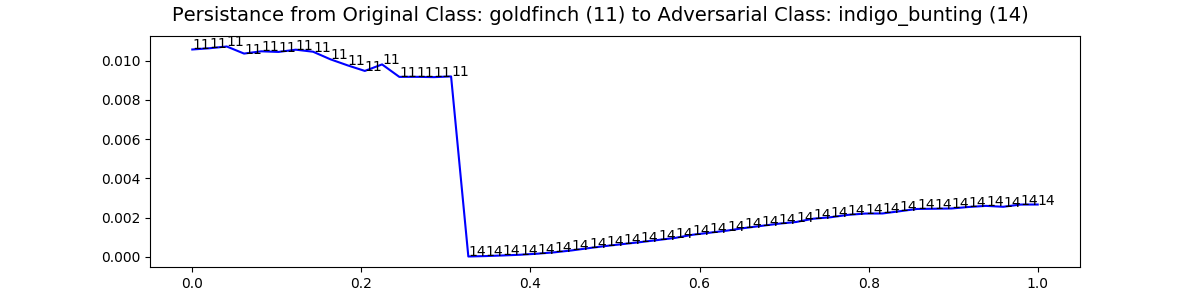
\includegraphics[width = \textwidth]
{c3_figures/persistence_interpolation-IMNET-class-11-vgg16-BIM-48-attack_data-001.png}
\caption{The $0.7$-persistence of images along the straight line path from an image in class \texttt{goldfinch} (11) to an adversarial image generated with BIM in the class \texttt{indigo\_bunting} (14) on a vgg16 classifier. The classification of each image on the straight line is listed as a number so that it is possible to see the transition from one class to another. The vertical axis is $0.7$-persistence and the horizontal axis is progress towards the adversarial image.}\label{fig:persistent_interpimage}
\end{figure}

An aggregation of persistence for many randomly selected images from the \texttt{goldfinch} class in the validation set for Imagenet are presented in Table \ref{TAB:PersistenceAlexVGG}. 
\begin{table}[!ht]
\centering


\begin{tabular}{llll}
\toprule
Network/Method & Avg Dist & Persist (Nat) & Persist (Adv) \\
\midrule
alexnet (total) & 0.0194 & 0.0155 & 0.0049 \\ 
\:\: BIM        & 0.0188 & 0.0162 & 0.0050 \\ 
\:\: MIFGSM     & 0.0240 & 0.0159 & 0.0053 \\ 
\:\: PGD        & 0.0188 & 0.0162 & 0.0050 \\ 
\midrule
vgg16   (total) & 0.0154 & 0.0146 & 0.0011 \\ 
\:\: BIM        & 0.0181 & 0.0145 & 0.0012 \\ 
\:\: MIFGSM     & 0.0238 & 0.0149 & 0.0018 \\ 
\:\: PGD        & 0.0181 & 0.0145 & 0.0012 \\ 
\bottomrule
\end{tabular}
\caption{The $0.7$-persistence values for natural (Nat) and
  adversarial (Adv) images along with average distortion for
  adversarial images of alexnet and vgg16 for attacks generated with
  BIM, MIFGSM, and PGD on images from class \texttt{goldfinch}
  targeted toward other classes from the ILSVRC 2015 classification
  labels.} \label{TAB:PersistenceAlexVGG}%\label{table:attack_pers} 
\end{table}
For each image of a \texttt{goldfinch} and for each network of alexnet and vgg16, attacks were prepared to a variety of 28 randomly selected targets using a BIM, MIFGSM, PGD, FGSM, R+FGSM, and CW attack strategies. The successful attacks were aggregated and their $0.7$-persistences were computed using the Bracketing Algorithm along with the $0.7$-persistences of the original images from which each attack was generated. Each attack strategy had a slightly different mixture of which source image and attack target combinations resulted in successful attacks. The overall rates for each are listed, as well as particular results on the most successful attack strategies in our experiments, BIM, MIFGSM, and PGD. The results indicate that adversarial images generated for these networks (alexnet and vgg16) using these attacks were less persistent, and hence less stable, than natural images for the same models. 



% % figure showing natural image
% \begin{figure}[p]
% \centering
% \includegraphics[width = \textwidth]
% %[trim=200 80 100 10,width = .95\textwidth]
% %trim=200 80 100 100, clip,width=15cm]
% {sampling_histograms/samplot_test.png}
% %{c3_figures/Image918-O1Anone_varx40.png}
% %%% Creator: Matplotlib, PGF backend
%%
%% To include the figure in your LaTeX document, write
%%   \input{<filename>.pgf}
%%
%% Make sure the required packages are loaded in your preamble
%%   \usepackage{pgf}
%%
%% and, on pdftex
%%   \usepackage[utf8]{inputenc}\DeclareUnicodeCharacter{2212}{-}
%%
%% or, on luatex and xetex
%%   \usepackage{unicode-math}
%%
%% Figures using additional raster images can only be included by \input if
%% they are in the same directory as the main LaTeX file. For loading figures
%% from other directories you can use the `import` package
%%   \usepackage{import}
%%
%% and then include the figures with
%%   \import{<path to file>}{<filename>.pgf}
%%
%% Matplotlib used the following preamble
%%   \usepackage{fontspec}
%%   \setmainfont{DejaVuSerif.ttf}[Path=C:/Users/glickenstein/anaconda3/lib/site-packages/matplotlib/mpl-data/fonts/ttf/]
%%   \setsansfont{DejaVuSans.ttf}[Path=C:/Users/glickenstein/anaconda3/lib/site-packages/matplotlib/mpl-data/fonts/ttf/]
%%   \setmonofont{DejaVuSansMono.ttf}[Path=C:/Users/glickenstein/anaconda3/lib/site-packages/matplotlib/mpl-data/fonts/ttf/]
%%
\begingroup%
\makeatletter%
\begin{pgfpicture}%
\pgfpathrectangle{\pgfpointorigin}{\pgfqpoint{5.000000in}{2.500000in}}%
\pgfusepath{use as bounding box, clip}%
\begin{pgfscope}%
\pgfsetbuttcap%
\pgfsetmiterjoin%
\definecolor{currentfill}{rgb}{1.000000,1.000000,1.000000}%
\pgfsetfillcolor{currentfill}%
\pgfsetlinewidth{0.000000pt}%
\definecolor{currentstroke}{rgb}{1.000000,1.000000,1.000000}%
\pgfsetstrokecolor{currentstroke}%
\pgfsetdash{}{0pt}%
\pgfpathmoveto{\pgfqpoint{0.000000in}{0.000000in}}%
\pgfpathlineto{\pgfqpoint{5.000000in}{0.000000in}}%
\pgfpathlineto{\pgfqpoint{5.000000in}{2.500000in}}%
\pgfpathlineto{\pgfqpoint{0.000000in}{2.500000in}}%
\pgfpathclose%
\pgfusepath{fill}%
\end{pgfscope}%
\begin{pgfscope}%
\pgfsetbuttcap%
\pgfsetmiterjoin%
\definecolor{currentfill}{rgb}{1.000000,1.000000,1.000000}%
\pgfsetfillcolor{currentfill}%
\pgfsetlinewidth{0.000000pt}%
\definecolor{currentstroke}{rgb}{0.000000,0.000000,0.000000}%
\pgfsetstrokecolor{currentstroke}%
\pgfsetstrokeopacity{0.000000}%
\pgfsetdash{}{0pt}%
\pgfpathmoveto{\pgfqpoint{0.300000in}{1.350000in}}%
\pgfpathlineto{\pgfqpoint{4.950000in}{1.350000in}}%
\pgfpathlineto{\pgfqpoint{4.950000in}{2.475000in}}%
\pgfpathlineto{\pgfqpoint{0.300000in}{2.475000in}}%
\pgfpathclose%
\pgfusepath{fill}%
\end{pgfscope}%
\begin{pgfscope}%
\pgfsetbuttcap%
\pgfsetroundjoin%
\definecolor{currentfill}{rgb}{0.000000,0.000000,0.000000}%
\pgfsetfillcolor{currentfill}%
\pgfsetlinewidth{0.803000pt}%
\definecolor{currentstroke}{rgb}{0.000000,0.000000,0.000000}%
\pgfsetstrokecolor{currentstroke}%
\pgfsetdash{}{0pt}%
\pgfsys@defobject{currentmarker}{\pgfqpoint{0.000000in}{-0.048611in}}{\pgfqpoint{0.000000in}{0.000000in}}{%
\pgfpathmoveto{\pgfqpoint{0.000000in}{0.000000in}}%
\pgfpathlineto{\pgfqpoint{0.000000in}{-0.048611in}}%
\pgfusepath{stroke,fill}%
}%
\begin{pgfscope}%
\pgfsys@transformshift{0.511364in}{1.350000in}%
\pgfsys@useobject{currentmarker}{}%
\end{pgfscope}%
\end{pgfscope}%
\begin{pgfscope}%
\definecolor{textcolor}{rgb}{0.000000,0.000000,0.000000}%
\pgfsetstrokecolor{textcolor}%
\pgfsetfillcolor{textcolor}%
\pgftext[x=0.511364in,y=1.252778in,,top]{\color{textcolor}\sffamily\fontsize{16.000000}{19.200000}\selectfont 0.0}%
\end{pgfscope}%
\begin{pgfscope}%
\pgfsetbuttcap%
\pgfsetroundjoin%
\definecolor{currentfill}{rgb}{0.000000,0.000000,0.000000}%
\pgfsetfillcolor{currentfill}%
\pgfsetlinewidth{0.803000pt}%
\definecolor{currentstroke}{rgb}{0.000000,0.000000,0.000000}%
\pgfsetstrokecolor{currentstroke}%
\pgfsetdash{}{0pt}%
\pgfsys@defobject{currentmarker}{\pgfqpoint{0.000000in}{-0.048611in}}{\pgfqpoint{0.000000in}{0.000000in}}{%
\pgfpathmoveto{\pgfqpoint{0.000000in}{0.000000in}}%
\pgfpathlineto{\pgfqpoint{0.000000in}{-0.048611in}}%
\pgfusepath{stroke,fill}%
}%
\begin{pgfscope}%
\pgfsys@transformshift{1.356818in}{1.350000in}%
\pgfsys@useobject{currentmarker}{}%
\end{pgfscope}%
\end{pgfscope}%
\begin{pgfscope}%
\definecolor{textcolor}{rgb}{0.000000,0.000000,0.000000}%
\pgfsetstrokecolor{textcolor}%
\pgfsetfillcolor{textcolor}%
\pgftext[x=1.356818in,y=1.252778in,,top]{\color{textcolor}\sffamily\fontsize{16.000000}{19.200000}\selectfont 0.2}%
\end{pgfscope}%
\begin{pgfscope}%
\pgfsetbuttcap%
\pgfsetroundjoin%
\definecolor{currentfill}{rgb}{0.000000,0.000000,0.000000}%
\pgfsetfillcolor{currentfill}%
\pgfsetlinewidth{0.803000pt}%
\definecolor{currentstroke}{rgb}{0.000000,0.000000,0.000000}%
\pgfsetstrokecolor{currentstroke}%
\pgfsetdash{}{0pt}%
\pgfsys@defobject{currentmarker}{\pgfqpoint{0.000000in}{-0.048611in}}{\pgfqpoint{0.000000in}{0.000000in}}{%
\pgfpathmoveto{\pgfqpoint{0.000000in}{0.000000in}}%
\pgfpathlineto{\pgfqpoint{0.000000in}{-0.048611in}}%
\pgfusepath{stroke,fill}%
}%
\begin{pgfscope}%
\pgfsys@transformshift{2.202273in}{1.350000in}%
\pgfsys@useobject{currentmarker}{}%
\end{pgfscope}%
\end{pgfscope}%
\begin{pgfscope}%
\definecolor{textcolor}{rgb}{0.000000,0.000000,0.000000}%
\pgfsetstrokecolor{textcolor}%
\pgfsetfillcolor{textcolor}%
\pgftext[x=2.202273in,y=1.252778in,,top]{\color{textcolor}\sffamily\fontsize{16.000000}{19.200000}\selectfont 0.4}%
\end{pgfscope}%
\begin{pgfscope}%
\pgfsetbuttcap%
\pgfsetroundjoin%
\definecolor{currentfill}{rgb}{0.000000,0.000000,0.000000}%
\pgfsetfillcolor{currentfill}%
\pgfsetlinewidth{0.803000pt}%
\definecolor{currentstroke}{rgb}{0.000000,0.000000,0.000000}%
\pgfsetstrokecolor{currentstroke}%
\pgfsetdash{}{0pt}%
\pgfsys@defobject{currentmarker}{\pgfqpoint{0.000000in}{-0.048611in}}{\pgfqpoint{0.000000in}{0.000000in}}{%
\pgfpathmoveto{\pgfqpoint{0.000000in}{0.000000in}}%
\pgfpathlineto{\pgfqpoint{0.000000in}{-0.048611in}}%
\pgfusepath{stroke,fill}%
}%
\begin{pgfscope}%
\pgfsys@transformshift{3.047727in}{1.350000in}%
\pgfsys@useobject{currentmarker}{}%
\end{pgfscope}%
\end{pgfscope}%
\begin{pgfscope}%
\definecolor{textcolor}{rgb}{0.000000,0.000000,0.000000}%
\pgfsetstrokecolor{textcolor}%
\pgfsetfillcolor{textcolor}%
\pgftext[x=3.047727in,y=1.252778in,,top]{\color{textcolor}\sffamily\fontsize{16.000000}{19.200000}\selectfont 0.6}%
\end{pgfscope}%
\begin{pgfscope}%
\pgfsetbuttcap%
\pgfsetroundjoin%
\definecolor{currentfill}{rgb}{0.000000,0.000000,0.000000}%
\pgfsetfillcolor{currentfill}%
\pgfsetlinewidth{0.803000pt}%
\definecolor{currentstroke}{rgb}{0.000000,0.000000,0.000000}%
\pgfsetstrokecolor{currentstroke}%
\pgfsetdash{}{0pt}%
\pgfsys@defobject{currentmarker}{\pgfqpoint{0.000000in}{-0.048611in}}{\pgfqpoint{0.000000in}{0.000000in}}{%
\pgfpathmoveto{\pgfqpoint{0.000000in}{0.000000in}}%
\pgfpathlineto{\pgfqpoint{0.000000in}{-0.048611in}}%
\pgfusepath{stroke,fill}%
}%
\begin{pgfscope}%
\pgfsys@transformshift{3.893182in}{1.350000in}%
\pgfsys@useobject{currentmarker}{}%
\end{pgfscope}%
\end{pgfscope}%
\begin{pgfscope}%
\definecolor{textcolor}{rgb}{0.000000,0.000000,0.000000}%
\pgfsetstrokecolor{textcolor}%
\pgfsetfillcolor{textcolor}%
\pgftext[x=3.893182in,y=1.252778in,,top]{\color{textcolor}\sffamily\fontsize{16.000000}{19.200000}\selectfont 0.8}%
\end{pgfscope}%
\begin{pgfscope}%
\pgfsetbuttcap%
\pgfsetroundjoin%
\definecolor{currentfill}{rgb}{0.000000,0.000000,0.000000}%
\pgfsetfillcolor{currentfill}%
\pgfsetlinewidth{0.803000pt}%
\definecolor{currentstroke}{rgb}{0.000000,0.000000,0.000000}%
\pgfsetstrokecolor{currentstroke}%
\pgfsetdash{}{0pt}%
\pgfsys@defobject{currentmarker}{\pgfqpoint{0.000000in}{-0.048611in}}{\pgfqpoint{0.000000in}{0.000000in}}{%
\pgfpathmoveto{\pgfqpoint{0.000000in}{0.000000in}}%
\pgfpathlineto{\pgfqpoint{0.000000in}{-0.048611in}}%
\pgfusepath{stroke,fill}%
}%
\begin{pgfscope}%
\pgfsys@transformshift{4.738636in}{1.350000in}%
\pgfsys@useobject{currentmarker}{}%
\end{pgfscope}%
\end{pgfscope}%
\begin{pgfscope}%
\definecolor{textcolor}{rgb}{0.000000,0.000000,0.000000}%
\pgfsetstrokecolor{textcolor}%
\pgfsetfillcolor{textcolor}%
\pgftext[x=4.738636in,y=1.252778in,,top]{\color{textcolor}\sffamily\fontsize{16.000000}{19.200000}\selectfont 1.0}%
\end{pgfscope}%
\begin{pgfscope}%
\definecolor{textcolor}{rgb}{0.000000,0.000000,0.000000}%
\pgfsetstrokecolor{textcolor}%
\pgfsetfillcolor{textcolor}%
\pgftext[x=2.625000in,y=0.982162in,,top]{\color{textcolor}\sffamily\fontsize{16.000000}{19.200000}\selectfont Standard Deviation (\(\displaystyle \sigma\))}%
\end{pgfscope}%
\begin{pgfscope}%
\pgfsetbuttcap%
\pgfsetroundjoin%
\definecolor{currentfill}{rgb}{0.000000,0.000000,0.000000}%
\pgfsetfillcolor{currentfill}%
\pgfsetlinewidth{0.803000pt}%
\definecolor{currentstroke}{rgb}{0.000000,0.000000,0.000000}%
\pgfsetstrokecolor{currentstroke}%
\pgfsetdash{}{0pt}%
\pgfsys@defobject{currentmarker}{\pgfqpoint{-0.048611in}{0.000000in}}{\pgfqpoint{0.000000in}{0.000000in}}{%
\pgfpathmoveto{\pgfqpoint{0.000000in}{0.000000in}}%
\pgfpathlineto{\pgfqpoint{-0.048611in}{0.000000in}}%
\pgfusepath{stroke,fill}%
}%
\begin{pgfscope}%
\pgfsys@transformshift{0.300000in}{1.401136in}%
\pgfsys@useobject{currentmarker}{}%
\end{pgfscope}%
\end{pgfscope}%
\begin{pgfscope}%
\definecolor{textcolor}{rgb}{0.000000,0.000000,0.000000}%
\pgfsetstrokecolor{textcolor}%
\pgfsetfillcolor{textcolor}%
\pgftext[x=0.061393in, y=1.316718in, left, base]{\color{textcolor}\sffamily\fontsize{16.000000}{19.200000}\selectfont 0}%
\end{pgfscope}%
\begin{pgfscope}%
\pgfsetbuttcap%
\pgfsetroundjoin%
\definecolor{currentfill}{rgb}{0.000000,0.000000,0.000000}%
\pgfsetfillcolor{currentfill}%
\pgfsetlinewidth{0.803000pt}%
\definecolor{currentstroke}{rgb}{0.000000,0.000000,0.000000}%
\pgfsetstrokecolor{currentstroke}%
\pgfsetdash{}{0pt}%
\pgfsys@defobject{currentmarker}{\pgfqpoint{-0.048611in}{0.000000in}}{\pgfqpoint{0.000000in}{0.000000in}}{%
\pgfpathmoveto{\pgfqpoint{0.000000in}{0.000000in}}%
\pgfpathlineto{\pgfqpoint{-0.048611in}{0.000000in}}%
\pgfusepath{stroke,fill}%
}%
\begin{pgfscope}%
\pgfsys@transformshift{0.300000in}{2.423864in}%
\pgfsys@useobject{currentmarker}{}%
\end{pgfscope}%
\end{pgfscope}%
\begin{pgfscope}%
\definecolor{textcolor}{rgb}{0.000000,0.000000,0.000000}%
\pgfsetstrokecolor{textcolor}%
\pgfsetfillcolor{textcolor}%
\pgftext[x=-0.221376in, y=2.339445in, left, base]{\color{textcolor}\sffamily\fontsize{16.000000}{19.200000}\selectfont 100}%
\end{pgfscope}%
\begin{pgfscope}%
\definecolor{textcolor}{rgb}{0.000000,0.000000,0.000000}%
\pgfsetstrokecolor{textcolor}%
\pgfsetfillcolor{textcolor}%
\pgftext[x=-0.151931in,y=1.912500in,,bottom,rotate=90.000000]{\color{textcolor}\sffamily\fontsize{16.000000}{19.200000}\selectfont Count}%
\end{pgfscope}%
\begin{pgfscope}%
\pgfpathrectangle{\pgfqpoint{0.300000in}{1.350000in}}{\pgfqpoint{4.650000in}{1.125000in}}%
\pgfusepath{clip}%
\pgfsetrectcap%
\pgfsetroundjoin%
\pgfsetlinewidth{1.003750pt}%
\definecolor{currentstroke}{rgb}{0.000000,0.000000,1.000000}%
\pgfsetstrokecolor{currentstroke}%
\pgfsetstrokeopacity{0.200000}%
\pgfsetdash{}{0pt}%
\pgfpathmoveto{\pgfqpoint{0.511364in}{1.401136in}}%
\pgfpathlineto{\pgfqpoint{2.848047in}{1.401136in}}%
\pgfpathlineto{\pgfqpoint{2.869290in}{1.411364in}}%
\pgfpathlineto{\pgfqpoint{2.890532in}{1.401136in}}%
\pgfpathlineto{\pgfqpoint{2.954260in}{1.401136in}}%
\pgfpathlineto{\pgfqpoint{2.996745in}{1.421591in}}%
\pgfpathlineto{\pgfqpoint{3.017988in}{1.401136in}}%
\pgfpathlineto{\pgfqpoint{3.039230in}{1.401136in}}%
\pgfpathlineto{\pgfqpoint{3.060473in}{1.411364in}}%
\pgfpathlineto{\pgfqpoint{3.081715in}{1.401136in}}%
\pgfpathlineto{\pgfqpoint{3.102958in}{1.401136in}}%
\pgfpathlineto{\pgfqpoint{3.124201in}{1.411364in}}%
\pgfpathlineto{\pgfqpoint{3.145443in}{1.401136in}}%
\pgfpathlineto{\pgfqpoint{3.357869in}{1.401136in}}%
\pgfpathlineto{\pgfqpoint{3.379111in}{1.421591in}}%
\pgfpathlineto{\pgfqpoint{3.400354in}{1.401136in}}%
\pgfpathlineto{\pgfqpoint{3.506567in}{1.401136in}}%
\pgfpathlineto{\pgfqpoint{3.527810in}{1.411364in}}%
\pgfpathlineto{\pgfqpoint{3.549052in}{1.401136in}}%
\pgfpathlineto{\pgfqpoint{3.634022in}{1.401136in}}%
\pgfpathlineto{\pgfqpoint{3.655265in}{1.411364in}}%
\pgfpathlineto{\pgfqpoint{3.676508in}{1.401136in}}%
\pgfpathlineto{\pgfqpoint{3.697750in}{1.431818in}}%
\pgfpathlineto{\pgfqpoint{3.761478in}{1.401136in}}%
\pgfpathlineto{\pgfqpoint{3.782720in}{1.431818in}}%
\pgfpathlineto{\pgfqpoint{3.803963in}{1.401136in}}%
\pgfpathlineto{\pgfqpoint{3.825206in}{1.401136in}}%
\pgfpathlineto{\pgfqpoint{3.846448in}{1.411364in}}%
\pgfpathlineto{\pgfqpoint{3.867691in}{1.401136in}}%
\pgfpathlineto{\pgfqpoint{3.888933in}{1.411364in}}%
\pgfpathlineto{\pgfqpoint{3.910176in}{1.401136in}}%
\pgfpathlineto{\pgfqpoint{3.931418in}{1.411364in}}%
\pgfpathlineto{\pgfqpoint{3.952661in}{1.401136in}}%
\pgfpathlineto{\pgfqpoint{3.973904in}{1.421591in}}%
\pgfpathlineto{\pgfqpoint{3.995146in}{1.421591in}}%
\pgfpathlineto{\pgfqpoint{4.016389in}{1.411364in}}%
\pgfpathlineto{\pgfqpoint{4.037631in}{1.411364in}}%
\pgfpathlineto{\pgfqpoint{4.058874in}{1.401136in}}%
\pgfpathlineto{\pgfqpoint{4.080116in}{1.411364in}}%
\pgfpathlineto{\pgfqpoint{4.101359in}{1.401136in}}%
\pgfpathlineto{\pgfqpoint{4.122602in}{1.411364in}}%
\pgfpathlineto{\pgfqpoint{4.143844in}{1.431818in}}%
\pgfpathlineto{\pgfqpoint{4.165087in}{1.421591in}}%
\pgfpathlineto{\pgfqpoint{4.186329in}{1.421591in}}%
\pgfpathlineto{\pgfqpoint{4.207572in}{1.401136in}}%
\pgfpathlineto{\pgfqpoint{4.228815in}{1.401136in}}%
\pgfpathlineto{\pgfqpoint{4.250057in}{1.421591in}}%
\pgfpathlineto{\pgfqpoint{4.271300in}{1.421591in}}%
\pgfpathlineto{\pgfqpoint{4.292542in}{1.401136in}}%
\pgfpathlineto{\pgfqpoint{4.313785in}{1.411364in}}%
\pgfpathlineto{\pgfqpoint{4.335027in}{1.411364in}}%
\pgfpathlineto{\pgfqpoint{4.356270in}{1.421591in}}%
\pgfpathlineto{\pgfqpoint{4.377513in}{1.411364in}}%
\pgfpathlineto{\pgfqpoint{4.398755in}{1.421591in}}%
\pgfpathlineto{\pgfqpoint{4.419998in}{1.411364in}}%
\pgfpathlineto{\pgfqpoint{4.441240in}{1.411364in}}%
\pgfpathlineto{\pgfqpoint{4.462483in}{1.442045in}}%
\pgfpathlineto{\pgfqpoint{4.483725in}{1.421591in}}%
\pgfpathlineto{\pgfqpoint{4.504968in}{1.442045in}}%
\pgfpathlineto{\pgfqpoint{4.526211in}{1.401136in}}%
\pgfpathlineto{\pgfqpoint{4.547453in}{1.401136in}}%
\pgfpathlineto{\pgfqpoint{4.568696in}{1.431818in}}%
\pgfpathlineto{\pgfqpoint{4.589938in}{1.421591in}}%
\pgfpathlineto{\pgfqpoint{4.611181in}{1.421591in}}%
\pgfpathlineto{\pgfqpoint{4.632423in}{1.401136in}}%
\pgfpathlineto{\pgfqpoint{4.674909in}{1.442045in}}%
\pgfpathlineto{\pgfqpoint{4.696151in}{1.421591in}}%
\pgfpathlineto{\pgfqpoint{4.717394in}{1.421591in}}%
\pgfpathlineto{\pgfqpoint{4.738636in}{1.431818in}}%
\pgfpathlineto{\pgfqpoint{4.738636in}{1.431818in}}%
\pgfusepath{stroke}%
\end{pgfscope}%
\begin{pgfscope}%
\pgfpathrectangle{\pgfqpoint{0.300000in}{1.350000in}}{\pgfqpoint{4.650000in}{1.125000in}}%
\pgfusepath{clip}%
\pgfsetrectcap%
\pgfsetroundjoin%
\pgfsetlinewidth{1.003750pt}%
\definecolor{currentstroke}{rgb}{0.000000,0.000000,1.000000}%
\pgfsetstrokecolor{currentstroke}%
\pgfsetstrokeopacity{0.200000}%
\pgfsetdash{}{0pt}%
\pgfpathmoveto{\pgfqpoint{0.511364in}{1.401136in}}%
\pgfpathlineto{\pgfqpoint{3.187928in}{1.401136in}}%
\pgfpathlineto{\pgfqpoint{3.209171in}{1.411364in}}%
\pgfpathlineto{\pgfqpoint{3.230413in}{1.401136in}}%
\pgfpathlineto{\pgfqpoint{4.165087in}{1.401136in}}%
\pgfpathlineto{\pgfqpoint{4.186329in}{1.411364in}}%
\pgfpathlineto{\pgfqpoint{4.207572in}{1.401136in}}%
\pgfpathlineto{\pgfqpoint{4.377513in}{1.401136in}}%
\pgfpathlineto{\pgfqpoint{4.398755in}{1.411364in}}%
\pgfpathlineto{\pgfqpoint{4.419998in}{1.401136in}}%
\pgfpathlineto{\pgfqpoint{4.738636in}{1.401136in}}%
\pgfpathlineto{\pgfqpoint{4.738636in}{1.401136in}}%
\pgfusepath{stroke}%
\end{pgfscope}%
\begin{pgfscope}%
\pgfpathrectangle{\pgfqpoint{0.300000in}{1.350000in}}{\pgfqpoint{4.650000in}{1.125000in}}%
\pgfusepath{clip}%
\pgfsetrectcap%
\pgfsetroundjoin%
\pgfsetlinewidth{1.003750pt}%
\definecolor{currentstroke}{rgb}{0.000000,0.000000,1.000000}%
\pgfsetstrokecolor{currentstroke}%
\pgfsetstrokeopacity{0.200000}%
\pgfsetdash{}{0pt}%
\pgfpathmoveto{\pgfqpoint{0.511364in}{1.401136in}}%
\pgfpathlineto{\pgfqpoint{0.638819in}{1.401136in}}%
\pgfpathlineto{\pgfqpoint{0.660062in}{1.462500in}}%
\pgfpathlineto{\pgfqpoint{0.681304in}{1.503409in}}%
\pgfpathlineto{\pgfqpoint{0.702547in}{1.667045in}}%
\pgfpathlineto{\pgfqpoint{0.723789in}{1.769318in}}%
\pgfpathlineto{\pgfqpoint{0.766275in}{1.912500in}}%
\pgfpathlineto{\pgfqpoint{0.787517in}{1.973864in}}%
\pgfpathlineto{\pgfqpoint{0.808760in}{2.055682in}}%
\pgfpathlineto{\pgfqpoint{0.830002in}{2.004545in}}%
\pgfpathlineto{\pgfqpoint{0.851245in}{2.086364in}}%
\pgfpathlineto{\pgfqpoint{0.872487in}{2.076136in}}%
\pgfpathlineto{\pgfqpoint{0.893730in}{2.106818in}}%
\pgfpathlineto{\pgfqpoint{0.914973in}{2.076136in}}%
\pgfpathlineto{\pgfqpoint{0.936215in}{2.127273in}}%
\pgfpathlineto{\pgfqpoint{0.957458in}{2.076136in}}%
\pgfpathlineto{\pgfqpoint{0.978700in}{2.127273in}}%
\pgfpathlineto{\pgfqpoint{0.999943in}{2.106818in}}%
\pgfpathlineto{\pgfqpoint{1.021185in}{2.168182in}}%
\pgfpathlineto{\pgfqpoint{1.042428in}{2.250000in}}%
\pgfpathlineto{\pgfqpoint{1.063671in}{2.137500in}}%
\pgfpathlineto{\pgfqpoint{1.084913in}{2.096591in}}%
\pgfpathlineto{\pgfqpoint{1.106156in}{2.147727in}}%
\pgfpathlineto{\pgfqpoint{1.127398in}{2.147727in}}%
\pgfpathlineto{\pgfqpoint{1.148641in}{2.045455in}}%
\pgfpathlineto{\pgfqpoint{1.169884in}{2.219318in}}%
\pgfpathlineto{\pgfqpoint{1.191126in}{2.127273in}}%
\pgfpathlineto{\pgfqpoint{1.212369in}{2.168182in}}%
\pgfpathlineto{\pgfqpoint{1.233611in}{2.168182in}}%
\pgfpathlineto{\pgfqpoint{1.254854in}{2.127273in}}%
\pgfpathlineto{\pgfqpoint{1.276096in}{2.096591in}}%
\pgfpathlineto{\pgfqpoint{1.297339in}{2.035227in}}%
\pgfpathlineto{\pgfqpoint{1.318582in}{2.127273in}}%
\pgfpathlineto{\pgfqpoint{1.339824in}{2.076136in}}%
\pgfpathlineto{\pgfqpoint{1.361067in}{2.086364in}}%
\pgfpathlineto{\pgfqpoint{1.382309in}{2.035227in}}%
\pgfpathlineto{\pgfqpoint{1.403552in}{1.922727in}}%
\pgfpathlineto{\pgfqpoint{1.424794in}{1.892045in}}%
\pgfpathlineto{\pgfqpoint{1.446037in}{1.932955in}}%
\pgfpathlineto{\pgfqpoint{1.467280in}{2.014773in}}%
\pgfpathlineto{\pgfqpoint{1.488522in}{1.820455in}}%
\pgfpathlineto{\pgfqpoint{1.509765in}{1.861364in}}%
\pgfpathlineto{\pgfqpoint{1.531007in}{1.892045in}}%
\pgfpathlineto{\pgfqpoint{1.552250in}{1.789773in}}%
\pgfpathlineto{\pgfqpoint{1.573492in}{1.810227in}}%
\pgfpathlineto{\pgfqpoint{1.594735in}{1.779545in}}%
\pgfpathlineto{\pgfqpoint{1.615978in}{1.759091in}}%
\pgfpathlineto{\pgfqpoint{1.637220in}{1.707955in}}%
\pgfpathlineto{\pgfqpoint{1.658463in}{1.759091in}}%
\pgfpathlineto{\pgfqpoint{1.679705in}{1.738636in}}%
\pgfpathlineto{\pgfqpoint{1.700948in}{1.881818in}}%
\pgfpathlineto{\pgfqpoint{1.722190in}{1.738636in}}%
\pgfpathlineto{\pgfqpoint{1.743433in}{1.789773in}}%
\pgfpathlineto{\pgfqpoint{1.764676in}{1.738636in}}%
\pgfpathlineto{\pgfqpoint{1.785918in}{1.636364in}}%
\pgfpathlineto{\pgfqpoint{1.807161in}{1.626136in}}%
\pgfpathlineto{\pgfqpoint{1.849646in}{1.687500in}}%
\pgfpathlineto{\pgfqpoint{1.870889in}{1.707955in}}%
\pgfpathlineto{\pgfqpoint{1.892131in}{1.687500in}}%
\pgfpathlineto{\pgfqpoint{1.913374in}{1.677273in}}%
\pgfpathlineto{\pgfqpoint{1.934616in}{1.677273in}}%
\pgfpathlineto{\pgfqpoint{1.955859in}{1.667045in}}%
\pgfpathlineto{\pgfqpoint{1.977101in}{1.605682in}}%
\pgfpathlineto{\pgfqpoint{1.998344in}{1.646591in}}%
\pgfpathlineto{\pgfqpoint{2.019587in}{1.605682in}}%
\pgfpathlineto{\pgfqpoint{2.040829in}{1.636364in}}%
\pgfpathlineto{\pgfqpoint{2.062072in}{1.615909in}}%
\pgfpathlineto{\pgfqpoint{2.083314in}{1.605682in}}%
\pgfpathlineto{\pgfqpoint{2.104557in}{1.656818in}}%
\pgfpathlineto{\pgfqpoint{2.125799in}{1.595455in}}%
\pgfpathlineto{\pgfqpoint{2.147042in}{1.646591in}}%
\pgfpathlineto{\pgfqpoint{2.168285in}{1.564773in}}%
\pgfpathlineto{\pgfqpoint{2.189527in}{1.615909in}}%
\pgfpathlineto{\pgfqpoint{2.210770in}{1.544318in}}%
\pgfpathlineto{\pgfqpoint{2.232012in}{1.523864in}}%
\pgfpathlineto{\pgfqpoint{2.253255in}{1.605682in}}%
\pgfpathlineto{\pgfqpoint{2.274497in}{1.544318in}}%
\pgfpathlineto{\pgfqpoint{2.295740in}{1.585227in}}%
\pgfpathlineto{\pgfqpoint{2.316983in}{1.615909in}}%
\pgfpathlineto{\pgfqpoint{2.338225in}{1.605682in}}%
\pgfpathlineto{\pgfqpoint{2.359468in}{1.646591in}}%
\pgfpathlineto{\pgfqpoint{2.380710in}{1.615909in}}%
\pgfpathlineto{\pgfqpoint{2.401953in}{1.595455in}}%
\pgfpathlineto{\pgfqpoint{2.423196in}{1.554545in}}%
\pgfpathlineto{\pgfqpoint{2.444438in}{1.595455in}}%
\pgfpathlineto{\pgfqpoint{2.465681in}{1.523864in}}%
\pgfpathlineto{\pgfqpoint{2.486923in}{1.482955in}}%
\pgfpathlineto{\pgfqpoint{2.508166in}{1.554545in}}%
\pgfpathlineto{\pgfqpoint{2.529408in}{1.534091in}}%
\pgfpathlineto{\pgfqpoint{2.550651in}{1.595455in}}%
\pgfpathlineto{\pgfqpoint{2.571894in}{1.554545in}}%
\pgfpathlineto{\pgfqpoint{2.593136in}{1.482955in}}%
\pgfpathlineto{\pgfqpoint{2.614379in}{1.513636in}}%
\pgfpathlineto{\pgfqpoint{2.635621in}{1.554545in}}%
\pgfpathlineto{\pgfqpoint{2.656864in}{1.482955in}}%
\pgfpathlineto{\pgfqpoint{2.678106in}{1.595455in}}%
\pgfpathlineto{\pgfqpoint{2.699349in}{1.503409in}}%
\pgfpathlineto{\pgfqpoint{2.720592in}{1.503409in}}%
\pgfpathlineto{\pgfqpoint{2.741834in}{1.513636in}}%
\pgfpathlineto{\pgfqpoint{2.763077in}{1.544318in}}%
\pgfpathlineto{\pgfqpoint{2.784319in}{1.544318in}}%
\pgfpathlineto{\pgfqpoint{2.805562in}{1.513636in}}%
\pgfpathlineto{\pgfqpoint{2.826804in}{1.513636in}}%
\pgfpathlineto{\pgfqpoint{2.848047in}{1.472727in}}%
\pgfpathlineto{\pgfqpoint{2.869290in}{1.503409in}}%
\pgfpathlineto{\pgfqpoint{2.890532in}{1.544318in}}%
\pgfpathlineto{\pgfqpoint{2.911775in}{1.503409in}}%
\pgfpathlineto{\pgfqpoint{2.933017in}{1.513636in}}%
\pgfpathlineto{\pgfqpoint{2.954260in}{1.452273in}}%
\pgfpathlineto{\pgfqpoint{2.996745in}{1.472727in}}%
\pgfpathlineto{\pgfqpoint{3.017988in}{1.503409in}}%
\pgfpathlineto{\pgfqpoint{3.039230in}{1.462500in}}%
\pgfpathlineto{\pgfqpoint{3.060473in}{1.523864in}}%
\pgfpathlineto{\pgfqpoint{3.081715in}{1.462500in}}%
\pgfpathlineto{\pgfqpoint{3.102958in}{1.534091in}}%
\pgfpathlineto{\pgfqpoint{3.124201in}{1.482955in}}%
\pgfpathlineto{\pgfqpoint{3.145443in}{1.482955in}}%
\pgfpathlineto{\pgfqpoint{3.166686in}{1.472727in}}%
\pgfpathlineto{\pgfqpoint{3.187928in}{1.482955in}}%
\pgfpathlineto{\pgfqpoint{3.209171in}{1.503409in}}%
\pgfpathlineto{\pgfqpoint{3.230413in}{1.462500in}}%
\pgfpathlineto{\pgfqpoint{3.251656in}{1.442045in}}%
\pgfpathlineto{\pgfqpoint{3.272899in}{1.482955in}}%
\pgfpathlineto{\pgfqpoint{3.294141in}{1.462500in}}%
\pgfpathlineto{\pgfqpoint{3.315384in}{1.493182in}}%
\pgfpathlineto{\pgfqpoint{3.336626in}{1.462500in}}%
\pgfpathlineto{\pgfqpoint{3.357869in}{1.462500in}}%
\pgfpathlineto{\pgfqpoint{3.379111in}{1.431818in}}%
\pgfpathlineto{\pgfqpoint{3.400354in}{1.421591in}}%
\pgfpathlineto{\pgfqpoint{3.421597in}{1.462500in}}%
\pgfpathlineto{\pgfqpoint{3.442839in}{1.472727in}}%
\pgfpathlineto{\pgfqpoint{3.464082in}{1.442045in}}%
\pgfpathlineto{\pgfqpoint{3.485324in}{1.462500in}}%
\pgfpathlineto{\pgfqpoint{3.506567in}{1.452273in}}%
\pgfpathlineto{\pgfqpoint{3.527810in}{1.421591in}}%
\pgfpathlineto{\pgfqpoint{3.549052in}{1.431818in}}%
\pgfpathlineto{\pgfqpoint{3.570295in}{1.462500in}}%
\pgfpathlineto{\pgfqpoint{3.591537in}{1.431818in}}%
\pgfpathlineto{\pgfqpoint{3.612780in}{1.411364in}}%
\pgfpathlineto{\pgfqpoint{3.634022in}{1.452273in}}%
\pgfpathlineto{\pgfqpoint{3.655265in}{1.442045in}}%
\pgfpathlineto{\pgfqpoint{3.676508in}{1.472727in}}%
\pgfpathlineto{\pgfqpoint{3.697750in}{1.452273in}}%
\pgfpathlineto{\pgfqpoint{3.718993in}{1.421591in}}%
\pgfpathlineto{\pgfqpoint{3.740235in}{1.411364in}}%
\pgfpathlineto{\pgfqpoint{3.761478in}{1.442045in}}%
\pgfpathlineto{\pgfqpoint{3.782720in}{1.452273in}}%
\pgfpathlineto{\pgfqpoint{3.803963in}{1.421591in}}%
\pgfpathlineto{\pgfqpoint{3.825206in}{1.401136in}}%
\pgfpathlineto{\pgfqpoint{3.846448in}{1.411364in}}%
\pgfpathlineto{\pgfqpoint{3.867691in}{1.431818in}}%
\pgfpathlineto{\pgfqpoint{3.888933in}{1.411364in}}%
\pgfpathlineto{\pgfqpoint{3.910176in}{1.442045in}}%
\pgfpathlineto{\pgfqpoint{3.931418in}{1.421591in}}%
\pgfpathlineto{\pgfqpoint{3.952661in}{1.442045in}}%
\pgfpathlineto{\pgfqpoint{3.973904in}{1.411364in}}%
\pgfpathlineto{\pgfqpoint{3.995146in}{1.421591in}}%
\pgfpathlineto{\pgfqpoint{4.016389in}{1.442045in}}%
\pgfpathlineto{\pgfqpoint{4.058874in}{1.421591in}}%
\pgfpathlineto{\pgfqpoint{4.080116in}{1.431818in}}%
\pgfpathlineto{\pgfqpoint{4.101359in}{1.421591in}}%
\pgfpathlineto{\pgfqpoint{4.122602in}{1.421591in}}%
\pgfpathlineto{\pgfqpoint{4.143844in}{1.431818in}}%
\pgfpathlineto{\pgfqpoint{4.165087in}{1.411364in}}%
\pgfpathlineto{\pgfqpoint{4.186329in}{1.421591in}}%
\pgfpathlineto{\pgfqpoint{4.207572in}{1.401136in}}%
\pgfpathlineto{\pgfqpoint{4.228815in}{1.411364in}}%
\pgfpathlineto{\pgfqpoint{4.250057in}{1.431818in}}%
\pgfpathlineto{\pgfqpoint{4.271300in}{1.401136in}}%
\pgfpathlineto{\pgfqpoint{4.292542in}{1.411364in}}%
\pgfpathlineto{\pgfqpoint{4.313785in}{1.401136in}}%
\pgfpathlineto{\pgfqpoint{4.335027in}{1.411364in}}%
\pgfpathlineto{\pgfqpoint{4.356270in}{1.401136in}}%
\pgfpathlineto{\pgfqpoint{4.377513in}{1.411364in}}%
\pgfpathlineto{\pgfqpoint{4.398755in}{1.411364in}}%
\pgfpathlineto{\pgfqpoint{4.419998in}{1.421591in}}%
\pgfpathlineto{\pgfqpoint{4.441240in}{1.401136in}}%
\pgfpathlineto{\pgfqpoint{4.504968in}{1.401136in}}%
\pgfpathlineto{\pgfqpoint{4.526211in}{1.411364in}}%
\pgfpathlineto{\pgfqpoint{4.547453in}{1.411364in}}%
\pgfpathlineto{\pgfqpoint{4.568696in}{1.401136in}}%
\pgfpathlineto{\pgfqpoint{4.589938in}{1.401136in}}%
\pgfpathlineto{\pgfqpoint{4.611181in}{1.411364in}}%
\pgfpathlineto{\pgfqpoint{4.632423in}{1.401136in}}%
\pgfpathlineto{\pgfqpoint{4.717394in}{1.401136in}}%
\pgfpathlineto{\pgfqpoint{4.738636in}{1.411364in}}%
\pgfpathlineto{\pgfqpoint{4.738636in}{1.411364in}}%
\pgfusepath{stroke}%
\end{pgfscope}%
\begin{pgfscope}%
\pgfpathrectangle{\pgfqpoint{0.300000in}{1.350000in}}{\pgfqpoint{4.650000in}{1.125000in}}%
\pgfusepath{clip}%
\pgfsetrectcap%
\pgfsetroundjoin%
\pgfsetlinewidth{1.003750pt}%
\definecolor{currentstroke}{rgb}{0.000000,0.000000,1.000000}%
\pgfsetstrokecolor{currentstroke}%
\pgfsetstrokeopacity{0.200000}%
\pgfsetdash{}{0pt}%
\pgfpathmoveto{\pgfqpoint{0.511364in}{1.401136in}}%
\pgfpathlineto{\pgfqpoint{0.575091in}{1.401136in}}%
\pgfpathlineto{\pgfqpoint{0.596334in}{1.431818in}}%
\pgfpathlineto{\pgfqpoint{0.617577in}{1.452273in}}%
\pgfpathlineto{\pgfqpoint{0.638819in}{1.513636in}}%
\pgfpathlineto{\pgfqpoint{0.660062in}{1.513636in}}%
\pgfpathlineto{\pgfqpoint{0.681304in}{1.503409in}}%
\pgfpathlineto{\pgfqpoint{0.702547in}{1.503409in}}%
\pgfpathlineto{\pgfqpoint{0.723789in}{1.472727in}}%
\pgfpathlineto{\pgfqpoint{0.745032in}{1.421591in}}%
\pgfpathlineto{\pgfqpoint{0.766275in}{1.411364in}}%
\pgfpathlineto{\pgfqpoint{0.787517in}{1.411364in}}%
\pgfpathlineto{\pgfqpoint{0.808760in}{1.421591in}}%
\pgfpathlineto{\pgfqpoint{0.851245in}{1.401136in}}%
\pgfpathlineto{\pgfqpoint{0.914973in}{1.401136in}}%
\pgfpathlineto{\pgfqpoint{0.936215in}{1.411364in}}%
\pgfpathlineto{\pgfqpoint{0.957458in}{1.401136in}}%
\pgfpathlineto{\pgfqpoint{0.978700in}{1.411364in}}%
\pgfpathlineto{\pgfqpoint{0.999943in}{1.411364in}}%
\pgfpathlineto{\pgfqpoint{1.021185in}{1.401136in}}%
\pgfpathlineto{\pgfqpoint{1.127398in}{1.401136in}}%
\pgfpathlineto{\pgfqpoint{1.148641in}{1.411364in}}%
\pgfpathlineto{\pgfqpoint{1.169884in}{1.401136in}}%
\pgfpathlineto{\pgfqpoint{4.738636in}{1.401136in}}%
\pgfpathlineto{\pgfqpoint{4.738636in}{1.401136in}}%
\pgfusepath{stroke}%
\end{pgfscope}%
\begin{pgfscope}%
\pgfpathrectangle{\pgfqpoint{0.300000in}{1.350000in}}{\pgfqpoint{4.650000in}{1.125000in}}%
\pgfusepath{clip}%
\pgfsetrectcap%
\pgfsetroundjoin%
\pgfsetlinewidth{1.003750pt}%
\definecolor{currentstroke}{rgb}{0.000000,0.000000,1.000000}%
\pgfsetstrokecolor{currentstroke}%
\pgfsetstrokeopacity{0.200000}%
\pgfsetdash{}{0pt}%
\pgfpathmoveto{\pgfqpoint{0.511364in}{1.401136in}}%
\pgfpathlineto{\pgfqpoint{0.553849in}{1.401136in}}%
\pgfpathlineto{\pgfqpoint{0.575091in}{1.442045in}}%
\pgfpathlineto{\pgfqpoint{0.596334in}{1.442045in}}%
\pgfpathlineto{\pgfqpoint{0.617577in}{1.421591in}}%
\pgfpathlineto{\pgfqpoint{0.638819in}{1.544318in}}%
\pgfpathlineto{\pgfqpoint{0.660062in}{1.554545in}}%
\pgfpathlineto{\pgfqpoint{0.681304in}{1.544318in}}%
\pgfpathlineto{\pgfqpoint{0.702547in}{1.442045in}}%
\pgfpathlineto{\pgfqpoint{0.723789in}{1.411364in}}%
\pgfpathlineto{\pgfqpoint{0.745032in}{1.421591in}}%
\pgfpathlineto{\pgfqpoint{0.766275in}{1.401136in}}%
\pgfpathlineto{\pgfqpoint{4.738636in}{1.401136in}}%
\pgfpathlineto{\pgfqpoint{4.738636in}{1.401136in}}%
\pgfusepath{stroke}%
\end{pgfscope}%
\begin{pgfscope}%
\pgfpathrectangle{\pgfqpoint{0.300000in}{1.350000in}}{\pgfqpoint{4.650000in}{1.125000in}}%
\pgfusepath{clip}%
\pgfsetrectcap%
\pgfsetroundjoin%
\pgfsetlinewidth{1.003750pt}%
\definecolor{currentstroke}{rgb}{0.000000,0.000000,1.000000}%
\pgfsetstrokecolor{currentstroke}%
\pgfsetstrokeopacity{0.200000}%
\pgfsetdash{}{0pt}%
\pgfpathmoveto{\pgfqpoint{0.511364in}{1.401136in}}%
\pgfpathlineto{\pgfqpoint{2.040829in}{1.401136in}}%
\pgfpathlineto{\pgfqpoint{2.062072in}{1.411364in}}%
\pgfpathlineto{\pgfqpoint{2.083314in}{1.401136in}}%
\pgfpathlineto{\pgfqpoint{2.189527in}{1.401136in}}%
\pgfpathlineto{\pgfqpoint{2.210770in}{1.411364in}}%
\pgfpathlineto{\pgfqpoint{2.232012in}{1.401136in}}%
\pgfpathlineto{\pgfqpoint{2.253255in}{1.401136in}}%
\pgfpathlineto{\pgfqpoint{2.274497in}{1.411364in}}%
\pgfpathlineto{\pgfqpoint{2.295740in}{1.401136in}}%
\pgfpathlineto{\pgfqpoint{2.316983in}{1.401136in}}%
\pgfpathlineto{\pgfqpoint{2.338225in}{1.431818in}}%
\pgfpathlineto{\pgfqpoint{2.359468in}{1.411364in}}%
\pgfpathlineto{\pgfqpoint{2.380710in}{1.401136in}}%
\pgfpathlineto{\pgfqpoint{2.423196in}{1.401136in}}%
\pgfpathlineto{\pgfqpoint{2.444438in}{1.411364in}}%
\pgfpathlineto{\pgfqpoint{2.465681in}{1.401136in}}%
\pgfpathlineto{\pgfqpoint{2.486923in}{1.431818in}}%
\pgfpathlineto{\pgfqpoint{2.508166in}{1.411364in}}%
\pgfpathlineto{\pgfqpoint{2.571894in}{1.442045in}}%
\pgfpathlineto{\pgfqpoint{2.593136in}{1.401136in}}%
\pgfpathlineto{\pgfqpoint{2.614379in}{1.401136in}}%
\pgfpathlineto{\pgfqpoint{2.635621in}{1.442045in}}%
\pgfpathlineto{\pgfqpoint{2.656864in}{1.411364in}}%
\pgfpathlineto{\pgfqpoint{2.678106in}{1.431818in}}%
\pgfpathlineto{\pgfqpoint{2.699349in}{1.431818in}}%
\pgfpathlineto{\pgfqpoint{2.741834in}{1.452273in}}%
\pgfpathlineto{\pgfqpoint{2.763077in}{1.411364in}}%
\pgfpathlineto{\pgfqpoint{2.784319in}{1.421591in}}%
\pgfpathlineto{\pgfqpoint{2.826804in}{1.421591in}}%
\pgfpathlineto{\pgfqpoint{2.848047in}{1.452273in}}%
\pgfpathlineto{\pgfqpoint{2.869290in}{1.462500in}}%
\pgfpathlineto{\pgfqpoint{2.890532in}{1.452273in}}%
\pgfpathlineto{\pgfqpoint{2.911775in}{1.411364in}}%
\pgfpathlineto{\pgfqpoint{2.933017in}{1.431818in}}%
\pgfpathlineto{\pgfqpoint{2.954260in}{1.442045in}}%
\pgfpathlineto{\pgfqpoint{2.975503in}{1.482955in}}%
\pgfpathlineto{\pgfqpoint{2.996745in}{1.452273in}}%
\pgfpathlineto{\pgfqpoint{3.017988in}{1.442045in}}%
\pgfpathlineto{\pgfqpoint{3.039230in}{1.411364in}}%
\pgfpathlineto{\pgfqpoint{3.060473in}{1.462500in}}%
\pgfpathlineto{\pgfqpoint{3.081715in}{1.462500in}}%
\pgfpathlineto{\pgfqpoint{3.102958in}{1.431818in}}%
\pgfpathlineto{\pgfqpoint{3.124201in}{1.442045in}}%
\pgfpathlineto{\pgfqpoint{3.145443in}{1.493182in}}%
\pgfpathlineto{\pgfqpoint{3.166686in}{1.442045in}}%
\pgfpathlineto{\pgfqpoint{3.187928in}{1.493182in}}%
\pgfpathlineto{\pgfqpoint{3.209171in}{1.431818in}}%
\pgfpathlineto{\pgfqpoint{3.230413in}{1.411364in}}%
\pgfpathlineto{\pgfqpoint{3.251656in}{1.431818in}}%
\pgfpathlineto{\pgfqpoint{3.272899in}{1.442045in}}%
\pgfpathlineto{\pgfqpoint{3.294141in}{1.472727in}}%
\pgfpathlineto{\pgfqpoint{3.315384in}{1.421591in}}%
\pgfpathlineto{\pgfqpoint{3.336626in}{1.421591in}}%
\pgfpathlineto{\pgfqpoint{3.357869in}{1.462500in}}%
\pgfpathlineto{\pgfqpoint{3.379111in}{1.421591in}}%
\pgfpathlineto{\pgfqpoint{3.400354in}{1.442045in}}%
\pgfpathlineto{\pgfqpoint{3.421597in}{1.472727in}}%
\pgfpathlineto{\pgfqpoint{3.442839in}{1.431818in}}%
\pgfpathlineto{\pgfqpoint{3.464082in}{1.472727in}}%
\pgfpathlineto{\pgfqpoint{3.485324in}{1.452273in}}%
\pgfpathlineto{\pgfqpoint{3.506567in}{1.421591in}}%
\pgfpathlineto{\pgfqpoint{3.527810in}{1.431818in}}%
\pgfpathlineto{\pgfqpoint{3.549052in}{1.472727in}}%
\pgfpathlineto{\pgfqpoint{3.570295in}{1.442045in}}%
\pgfpathlineto{\pgfqpoint{3.591537in}{1.452273in}}%
\pgfpathlineto{\pgfqpoint{3.612780in}{1.431818in}}%
\pgfpathlineto{\pgfqpoint{3.634022in}{1.462500in}}%
\pgfpathlineto{\pgfqpoint{3.655265in}{1.411364in}}%
\pgfpathlineto{\pgfqpoint{3.676508in}{1.431818in}}%
\pgfpathlineto{\pgfqpoint{3.697750in}{1.421591in}}%
\pgfpathlineto{\pgfqpoint{3.718993in}{1.472727in}}%
\pgfpathlineto{\pgfqpoint{3.740235in}{1.503409in}}%
\pgfpathlineto{\pgfqpoint{3.761478in}{1.421591in}}%
\pgfpathlineto{\pgfqpoint{3.782720in}{1.421591in}}%
\pgfpathlineto{\pgfqpoint{3.803963in}{1.411364in}}%
\pgfpathlineto{\pgfqpoint{3.825206in}{1.442045in}}%
\pgfpathlineto{\pgfqpoint{3.888933in}{1.411364in}}%
\pgfpathlineto{\pgfqpoint{3.910176in}{1.411364in}}%
\pgfpathlineto{\pgfqpoint{3.931418in}{1.421591in}}%
\pgfpathlineto{\pgfqpoint{3.952661in}{1.411364in}}%
\pgfpathlineto{\pgfqpoint{3.973904in}{1.411364in}}%
\pgfpathlineto{\pgfqpoint{3.995146in}{1.442045in}}%
\pgfpathlineto{\pgfqpoint{4.016389in}{1.421591in}}%
\pgfpathlineto{\pgfqpoint{4.037631in}{1.421591in}}%
\pgfpathlineto{\pgfqpoint{4.058874in}{1.411364in}}%
\pgfpathlineto{\pgfqpoint{4.080116in}{1.421591in}}%
\pgfpathlineto{\pgfqpoint{4.101359in}{1.411364in}}%
\pgfpathlineto{\pgfqpoint{4.122602in}{1.411364in}}%
\pgfpathlineto{\pgfqpoint{4.143844in}{1.442045in}}%
\pgfpathlineto{\pgfqpoint{4.186329in}{1.421591in}}%
\pgfpathlineto{\pgfqpoint{4.207572in}{1.421591in}}%
\pgfpathlineto{\pgfqpoint{4.228815in}{1.431818in}}%
\pgfpathlineto{\pgfqpoint{4.250057in}{1.401136in}}%
\pgfpathlineto{\pgfqpoint{4.271300in}{1.431818in}}%
\pgfpathlineto{\pgfqpoint{4.292542in}{1.401136in}}%
\pgfpathlineto{\pgfqpoint{4.335027in}{1.421591in}}%
\pgfpathlineto{\pgfqpoint{4.356270in}{1.421591in}}%
\pgfpathlineto{\pgfqpoint{4.377513in}{1.401136in}}%
\pgfpathlineto{\pgfqpoint{4.398755in}{1.411364in}}%
\pgfpathlineto{\pgfqpoint{4.419998in}{1.401136in}}%
\pgfpathlineto{\pgfqpoint{4.441240in}{1.401136in}}%
\pgfpathlineto{\pgfqpoint{4.462483in}{1.411364in}}%
\pgfpathlineto{\pgfqpoint{4.483725in}{1.411364in}}%
\pgfpathlineto{\pgfqpoint{4.504968in}{1.401136in}}%
\pgfpathlineto{\pgfqpoint{4.526211in}{1.411364in}}%
\pgfpathlineto{\pgfqpoint{4.547453in}{1.401136in}}%
\pgfpathlineto{\pgfqpoint{4.589938in}{1.401136in}}%
\pgfpathlineto{\pgfqpoint{4.611181in}{1.411364in}}%
\pgfpathlineto{\pgfqpoint{4.632423in}{1.401136in}}%
\pgfpathlineto{\pgfqpoint{4.653666in}{1.411364in}}%
\pgfpathlineto{\pgfqpoint{4.674909in}{1.411364in}}%
\pgfpathlineto{\pgfqpoint{4.696151in}{1.431818in}}%
\pgfpathlineto{\pgfqpoint{4.717394in}{1.401136in}}%
\pgfpathlineto{\pgfqpoint{4.738636in}{1.401136in}}%
\pgfpathlineto{\pgfqpoint{4.738636in}{1.401136in}}%
\pgfusepath{stroke}%
\end{pgfscope}%
\begin{pgfscope}%
\pgfpathrectangle{\pgfqpoint{0.300000in}{1.350000in}}{\pgfqpoint{4.650000in}{1.125000in}}%
\pgfusepath{clip}%
\pgfsetrectcap%
\pgfsetroundjoin%
\pgfsetlinewidth{1.003750pt}%
\definecolor{currentstroke}{rgb}{0.000000,0.000000,1.000000}%
\pgfsetstrokecolor{currentstroke}%
\pgfsetstrokeopacity{0.200000}%
\pgfsetdash{}{0pt}%
\pgfpathmoveto{\pgfqpoint{0.511364in}{1.401136in}}%
\pgfpathlineto{\pgfqpoint{1.021185in}{1.401136in}}%
\pgfpathlineto{\pgfqpoint{1.042428in}{1.411364in}}%
\pgfpathlineto{\pgfqpoint{1.063671in}{1.411364in}}%
\pgfpathlineto{\pgfqpoint{1.084913in}{1.421591in}}%
\pgfpathlineto{\pgfqpoint{1.127398in}{1.401136in}}%
\pgfpathlineto{\pgfqpoint{1.148641in}{1.421591in}}%
\pgfpathlineto{\pgfqpoint{1.191126in}{1.421591in}}%
\pgfpathlineto{\pgfqpoint{1.212369in}{1.431818in}}%
\pgfpathlineto{\pgfqpoint{1.254854in}{1.411364in}}%
\pgfpathlineto{\pgfqpoint{1.297339in}{1.452273in}}%
\pgfpathlineto{\pgfqpoint{1.318582in}{1.421591in}}%
\pgfpathlineto{\pgfqpoint{1.339824in}{1.431818in}}%
\pgfpathlineto{\pgfqpoint{1.361067in}{1.411364in}}%
\pgfpathlineto{\pgfqpoint{1.382309in}{1.421591in}}%
\pgfpathlineto{\pgfqpoint{1.403552in}{1.442045in}}%
\pgfpathlineto{\pgfqpoint{1.424794in}{1.401136in}}%
\pgfpathlineto{\pgfqpoint{1.446037in}{1.401136in}}%
\pgfpathlineto{\pgfqpoint{1.467280in}{1.421591in}}%
\pgfpathlineto{\pgfqpoint{1.488522in}{1.421591in}}%
\pgfpathlineto{\pgfqpoint{1.509765in}{1.411364in}}%
\pgfpathlineto{\pgfqpoint{1.531007in}{1.411364in}}%
\pgfpathlineto{\pgfqpoint{1.573492in}{1.431818in}}%
\pgfpathlineto{\pgfqpoint{1.594735in}{1.421591in}}%
\pgfpathlineto{\pgfqpoint{1.637220in}{1.442045in}}%
\pgfpathlineto{\pgfqpoint{1.658463in}{1.411364in}}%
\pgfpathlineto{\pgfqpoint{1.679705in}{1.401136in}}%
\pgfpathlineto{\pgfqpoint{1.700948in}{1.421591in}}%
\pgfpathlineto{\pgfqpoint{1.722190in}{1.431818in}}%
\pgfpathlineto{\pgfqpoint{1.743433in}{1.421591in}}%
\pgfpathlineto{\pgfqpoint{1.764676in}{1.401136in}}%
\pgfpathlineto{\pgfqpoint{1.785918in}{1.411364in}}%
\pgfpathlineto{\pgfqpoint{1.807161in}{1.401136in}}%
\pgfpathlineto{\pgfqpoint{1.828403in}{1.411364in}}%
\pgfpathlineto{\pgfqpoint{1.892131in}{1.411364in}}%
\pgfpathlineto{\pgfqpoint{1.913374in}{1.401136in}}%
\pgfpathlineto{\pgfqpoint{1.934616in}{1.411364in}}%
\pgfpathlineto{\pgfqpoint{1.955859in}{1.401136in}}%
\pgfpathlineto{\pgfqpoint{2.125799in}{1.401136in}}%
\pgfpathlineto{\pgfqpoint{2.147042in}{1.411364in}}%
\pgfpathlineto{\pgfqpoint{2.168285in}{1.401136in}}%
\pgfpathlineto{\pgfqpoint{2.189527in}{1.401136in}}%
\pgfpathlineto{\pgfqpoint{2.210770in}{1.411364in}}%
\pgfpathlineto{\pgfqpoint{2.232012in}{1.401136in}}%
\pgfpathlineto{\pgfqpoint{2.338225in}{1.401136in}}%
\pgfpathlineto{\pgfqpoint{2.359468in}{1.411364in}}%
\pgfpathlineto{\pgfqpoint{2.380710in}{1.401136in}}%
\pgfpathlineto{\pgfqpoint{2.401953in}{1.411364in}}%
\pgfpathlineto{\pgfqpoint{2.423196in}{1.411364in}}%
\pgfpathlineto{\pgfqpoint{2.444438in}{1.401136in}}%
\pgfpathlineto{\pgfqpoint{2.465681in}{1.401136in}}%
\pgfpathlineto{\pgfqpoint{2.486923in}{1.411364in}}%
\pgfpathlineto{\pgfqpoint{2.508166in}{1.401136in}}%
\pgfpathlineto{\pgfqpoint{2.529408in}{1.411364in}}%
\pgfpathlineto{\pgfqpoint{2.550651in}{1.411364in}}%
\pgfpathlineto{\pgfqpoint{2.571894in}{1.401136in}}%
\pgfpathlineto{\pgfqpoint{2.614379in}{1.401136in}}%
\pgfpathlineto{\pgfqpoint{2.635621in}{1.411364in}}%
\pgfpathlineto{\pgfqpoint{2.656864in}{1.401136in}}%
\pgfpathlineto{\pgfqpoint{4.738636in}{1.401136in}}%
\pgfpathlineto{\pgfqpoint{4.738636in}{1.401136in}}%
\pgfusepath{stroke}%
\end{pgfscope}%
\begin{pgfscope}%
\pgfpathrectangle{\pgfqpoint{0.300000in}{1.350000in}}{\pgfqpoint{4.650000in}{1.125000in}}%
\pgfusepath{clip}%
\pgfsetrectcap%
\pgfsetroundjoin%
\pgfsetlinewidth{1.003750pt}%
\definecolor{currentstroke}{rgb}{0.000000,0.000000,1.000000}%
\pgfsetstrokecolor{currentstroke}%
\pgfsetstrokeopacity{0.200000}%
\pgfsetdash{}{0pt}%
\pgfpathmoveto{\pgfqpoint{0.511364in}{1.401136in}}%
\pgfpathlineto{\pgfqpoint{3.421597in}{1.401136in}}%
\pgfpathlineto{\pgfqpoint{3.442839in}{1.411364in}}%
\pgfpathlineto{\pgfqpoint{3.464082in}{1.401136in}}%
\pgfpathlineto{\pgfqpoint{3.867691in}{1.401136in}}%
\pgfpathlineto{\pgfqpoint{3.888933in}{1.411364in}}%
\pgfpathlineto{\pgfqpoint{3.910176in}{1.411364in}}%
\pgfpathlineto{\pgfqpoint{3.931418in}{1.401136in}}%
\pgfpathlineto{\pgfqpoint{4.738636in}{1.401136in}}%
\pgfpathlineto{\pgfqpoint{4.738636in}{1.401136in}}%
\pgfusepath{stroke}%
\end{pgfscope}%
\begin{pgfscope}%
\pgfpathrectangle{\pgfqpoint{0.300000in}{1.350000in}}{\pgfqpoint{4.650000in}{1.125000in}}%
\pgfusepath{clip}%
\pgfsetrectcap%
\pgfsetroundjoin%
\pgfsetlinewidth{1.003750pt}%
\definecolor{currentstroke}{rgb}{0.000000,0.000000,1.000000}%
\pgfsetstrokecolor{currentstroke}%
\pgfsetstrokeopacity{0.200000}%
\pgfsetdash{}{0pt}%
\pgfpathmoveto{\pgfqpoint{0.511364in}{1.401136in}}%
\pgfpathlineto{\pgfqpoint{0.745032in}{1.401136in}}%
\pgfpathlineto{\pgfqpoint{0.766275in}{1.411364in}}%
\pgfpathlineto{\pgfqpoint{0.787517in}{1.401136in}}%
\pgfpathlineto{\pgfqpoint{0.914973in}{1.401136in}}%
\pgfpathlineto{\pgfqpoint{0.936215in}{1.411364in}}%
\pgfpathlineto{\pgfqpoint{0.957458in}{1.411364in}}%
\pgfpathlineto{\pgfqpoint{0.978700in}{1.401136in}}%
\pgfpathlineto{\pgfqpoint{0.999943in}{1.401136in}}%
\pgfpathlineto{\pgfqpoint{1.021185in}{1.431818in}}%
\pgfpathlineto{\pgfqpoint{1.042428in}{1.401136in}}%
\pgfpathlineto{\pgfqpoint{1.084913in}{1.401136in}}%
\pgfpathlineto{\pgfqpoint{1.106156in}{1.411364in}}%
\pgfpathlineto{\pgfqpoint{1.148641in}{1.411364in}}%
\pgfpathlineto{\pgfqpoint{1.169884in}{1.401136in}}%
\pgfpathlineto{\pgfqpoint{1.212369in}{1.401136in}}%
\pgfpathlineto{\pgfqpoint{1.233611in}{1.411364in}}%
\pgfpathlineto{\pgfqpoint{1.254854in}{1.401136in}}%
\pgfpathlineto{\pgfqpoint{1.276096in}{1.401136in}}%
\pgfpathlineto{\pgfqpoint{1.297339in}{1.411364in}}%
\pgfpathlineto{\pgfqpoint{1.318582in}{1.401136in}}%
\pgfpathlineto{\pgfqpoint{1.339824in}{1.401136in}}%
\pgfpathlineto{\pgfqpoint{1.361067in}{1.421591in}}%
\pgfpathlineto{\pgfqpoint{1.382309in}{1.401136in}}%
\pgfpathlineto{\pgfqpoint{1.424794in}{1.401136in}}%
\pgfpathlineto{\pgfqpoint{1.446037in}{1.411364in}}%
\pgfpathlineto{\pgfqpoint{1.488522in}{1.411364in}}%
\pgfpathlineto{\pgfqpoint{1.509765in}{1.401136in}}%
\pgfpathlineto{\pgfqpoint{4.738636in}{1.401136in}}%
\pgfpathlineto{\pgfqpoint{4.738636in}{1.401136in}}%
\pgfusepath{stroke}%
\end{pgfscope}%
\begin{pgfscope}%
\pgfpathrectangle{\pgfqpoint{0.300000in}{1.350000in}}{\pgfqpoint{4.650000in}{1.125000in}}%
\pgfusepath{clip}%
\pgfsetrectcap%
\pgfsetroundjoin%
\pgfsetlinewidth{1.003750pt}%
\definecolor{currentstroke}{rgb}{0.000000,0.000000,1.000000}%
\pgfsetstrokecolor{currentstroke}%
\pgfsetstrokeopacity{0.200000}%
\pgfsetdash{}{0pt}%
\pgfpathmoveto{\pgfqpoint{0.511364in}{1.401136in}}%
\pgfpathlineto{\pgfqpoint{3.910176in}{1.401136in}}%
\pgfpathlineto{\pgfqpoint{3.931418in}{1.411364in}}%
\pgfpathlineto{\pgfqpoint{3.952661in}{1.401136in}}%
\pgfpathlineto{\pgfqpoint{4.738636in}{1.401136in}}%
\pgfpathlineto{\pgfqpoint{4.738636in}{1.401136in}}%
\pgfusepath{stroke}%
\end{pgfscope}%
\begin{pgfscope}%
\pgfpathrectangle{\pgfqpoint{0.300000in}{1.350000in}}{\pgfqpoint{4.650000in}{1.125000in}}%
\pgfusepath{clip}%
\pgfsetrectcap%
\pgfsetroundjoin%
\pgfsetlinewidth{1.003750pt}%
\definecolor{currentstroke}{rgb}{0.000000,0.000000,1.000000}%
\pgfsetstrokecolor{currentstroke}%
\pgfsetstrokeopacity{0.200000}%
\pgfsetdash{}{0pt}%
\pgfpathmoveto{\pgfqpoint{0.511364in}{2.423864in}}%
\pgfpathlineto{\pgfqpoint{0.553849in}{2.423864in}}%
\pgfpathlineto{\pgfqpoint{0.575091in}{2.311364in}}%
\pgfpathlineto{\pgfqpoint{0.596334in}{2.229545in}}%
\pgfpathlineto{\pgfqpoint{0.617577in}{2.168182in}}%
\pgfpathlineto{\pgfqpoint{0.660062in}{1.748864in}}%
\pgfpathlineto{\pgfqpoint{0.681304in}{1.636364in}}%
\pgfpathlineto{\pgfqpoint{0.702547in}{1.513636in}}%
\pgfpathlineto{\pgfqpoint{0.723789in}{1.421591in}}%
\pgfpathlineto{\pgfqpoint{0.745032in}{1.401136in}}%
\pgfpathlineto{\pgfqpoint{0.766275in}{1.411364in}}%
\pgfpathlineto{\pgfqpoint{0.787517in}{1.411364in}}%
\pgfpathlineto{\pgfqpoint{0.808760in}{1.401136in}}%
\pgfpathlineto{\pgfqpoint{4.738636in}{1.401136in}}%
\pgfpathlineto{\pgfqpoint{4.738636in}{1.401136in}}%
\pgfusepath{stroke}%
\end{pgfscope}%
\begin{pgfscope}%
\pgfpathrectangle{\pgfqpoint{0.300000in}{1.350000in}}{\pgfqpoint{4.650000in}{1.125000in}}%
\pgfusepath{clip}%
\pgfsetrectcap%
\pgfsetroundjoin%
\pgfsetlinewidth{1.003750pt}%
\definecolor{currentstroke}{rgb}{0.000000,0.000000,1.000000}%
\pgfsetstrokecolor{currentstroke}%
\pgfsetstrokeopacity{0.200000}%
\pgfsetdash{}{0pt}%
\pgfpathmoveto{\pgfqpoint{0.511364in}{1.401136in}}%
\pgfpathlineto{\pgfqpoint{3.294141in}{1.401136in}}%
\pgfpathlineto{\pgfqpoint{3.315384in}{1.411364in}}%
\pgfpathlineto{\pgfqpoint{3.336626in}{1.401136in}}%
\pgfpathlineto{\pgfqpoint{4.738636in}{1.401136in}}%
\pgfpathlineto{\pgfqpoint{4.738636in}{1.401136in}}%
\pgfusepath{stroke}%
\end{pgfscope}%
\begin{pgfscope}%
\pgfpathrectangle{\pgfqpoint{0.300000in}{1.350000in}}{\pgfqpoint{4.650000in}{1.125000in}}%
\pgfusepath{clip}%
\pgfsetrectcap%
\pgfsetroundjoin%
\pgfsetlinewidth{1.003750pt}%
\definecolor{currentstroke}{rgb}{0.000000,0.000000,1.000000}%
\pgfsetstrokecolor{currentstroke}%
\pgfsetstrokeopacity{0.200000}%
\pgfsetdash{}{0pt}%
\pgfpathmoveto{\pgfqpoint{0.511364in}{1.401136in}}%
\pgfpathlineto{\pgfqpoint{2.911775in}{1.401136in}}%
\pgfpathlineto{\pgfqpoint{2.933017in}{1.411364in}}%
\pgfpathlineto{\pgfqpoint{2.954260in}{1.401136in}}%
\pgfpathlineto{\pgfqpoint{2.996745in}{1.421591in}}%
\pgfpathlineto{\pgfqpoint{3.017988in}{1.401136in}}%
\pgfpathlineto{\pgfqpoint{3.060473in}{1.401136in}}%
\pgfpathlineto{\pgfqpoint{3.081715in}{1.431818in}}%
\pgfpathlineto{\pgfqpoint{3.102958in}{1.411364in}}%
\pgfpathlineto{\pgfqpoint{3.124201in}{1.401136in}}%
\pgfpathlineto{\pgfqpoint{3.145443in}{1.401136in}}%
\pgfpathlineto{\pgfqpoint{3.166686in}{1.411364in}}%
\pgfpathlineto{\pgfqpoint{3.187928in}{1.411364in}}%
\pgfpathlineto{\pgfqpoint{3.209171in}{1.431818in}}%
\pgfpathlineto{\pgfqpoint{3.230413in}{1.442045in}}%
\pgfpathlineto{\pgfqpoint{3.251656in}{1.431818in}}%
\pgfpathlineto{\pgfqpoint{3.272899in}{1.431818in}}%
\pgfpathlineto{\pgfqpoint{3.294141in}{1.401136in}}%
\pgfpathlineto{\pgfqpoint{3.315384in}{1.421591in}}%
\pgfpathlineto{\pgfqpoint{3.336626in}{1.421591in}}%
\pgfpathlineto{\pgfqpoint{3.357869in}{1.431818in}}%
\pgfpathlineto{\pgfqpoint{3.379111in}{1.452273in}}%
\pgfpathlineto{\pgfqpoint{3.400354in}{1.462500in}}%
\pgfpathlineto{\pgfqpoint{3.421597in}{1.431818in}}%
\pgfpathlineto{\pgfqpoint{3.442839in}{1.431818in}}%
\pgfpathlineto{\pgfqpoint{3.464082in}{1.462500in}}%
\pgfpathlineto{\pgfqpoint{3.485324in}{1.442045in}}%
\pgfpathlineto{\pgfqpoint{3.506567in}{1.472727in}}%
\pgfpathlineto{\pgfqpoint{3.527810in}{1.472727in}}%
\pgfpathlineto{\pgfqpoint{3.549052in}{1.442045in}}%
\pgfpathlineto{\pgfqpoint{3.591537in}{1.503409in}}%
\pgfpathlineto{\pgfqpoint{3.612780in}{1.472727in}}%
\pgfpathlineto{\pgfqpoint{3.634022in}{1.482955in}}%
\pgfpathlineto{\pgfqpoint{3.655265in}{1.534091in}}%
\pgfpathlineto{\pgfqpoint{3.676508in}{1.472727in}}%
\pgfpathlineto{\pgfqpoint{3.697750in}{1.534091in}}%
\pgfpathlineto{\pgfqpoint{3.718993in}{1.513636in}}%
\pgfpathlineto{\pgfqpoint{3.740235in}{1.523864in}}%
\pgfpathlineto{\pgfqpoint{3.761478in}{1.564773in}}%
\pgfpathlineto{\pgfqpoint{3.782720in}{1.554545in}}%
\pgfpathlineto{\pgfqpoint{3.825206in}{1.615909in}}%
\pgfpathlineto{\pgfqpoint{3.846448in}{1.564773in}}%
\pgfpathlineto{\pgfqpoint{3.867691in}{1.544318in}}%
\pgfpathlineto{\pgfqpoint{3.888933in}{1.575000in}}%
\pgfpathlineto{\pgfqpoint{3.910176in}{1.523864in}}%
\pgfpathlineto{\pgfqpoint{3.931418in}{1.554545in}}%
\pgfpathlineto{\pgfqpoint{3.952661in}{1.544318in}}%
\pgfpathlineto{\pgfqpoint{3.973904in}{1.595455in}}%
\pgfpathlineto{\pgfqpoint{3.995146in}{1.564773in}}%
\pgfpathlineto{\pgfqpoint{4.016389in}{1.575000in}}%
\pgfpathlineto{\pgfqpoint{4.037631in}{1.554545in}}%
\pgfpathlineto{\pgfqpoint{4.058874in}{1.595455in}}%
\pgfpathlineto{\pgfqpoint{4.080116in}{1.564773in}}%
\pgfpathlineto{\pgfqpoint{4.101359in}{1.656818in}}%
\pgfpathlineto{\pgfqpoint{4.122602in}{1.605682in}}%
\pgfpathlineto{\pgfqpoint{4.143844in}{1.646591in}}%
\pgfpathlineto{\pgfqpoint{4.165087in}{1.615909in}}%
\pgfpathlineto{\pgfqpoint{4.186329in}{1.605682in}}%
\pgfpathlineto{\pgfqpoint{4.207572in}{1.575000in}}%
\pgfpathlineto{\pgfqpoint{4.228815in}{1.718182in}}%
\pgfpathlineto{\pgfqpoint{4.250057in}{1.840909in}}%
\pgfpathlineto{\pgfqpoint{4.271300in}{1.728409in}}%
\pgfpathlineto{\pgfqpoint{4.292542in}{1.728409in}}%
\pgfpathlineto{\pgfqpoint{4.313785in}{1.687500in}}%
\pgfpathlineto{\pgfqpoint{4.335027in}{1.667045in}}%
\pgfpathlineto{\pgfqpoint{4.356270in}{1.748864in}}%
\pgfpathlineto{\pgfqpoint{4.377513in}{1.656818in}}%
\pgfpathlineto{\pgfqpoint{4.398755in}{1.789773in}}%
\pgfpathlineto{\pgfqpoint{4.419998in}{1.718182in}}%
\pgfpathlineto{\pgfqpoint{4.441240in}{1.779545in}}%
\pgfpathlineto{\pgfqpoint{4.462483in}{1.697727in}}%
\pgfpathlineto{\pgfqpoint{4.483725in}{1.697727in}}%
\pgfpathlineto{\pgfqpoint{4.504968in}{1.769318in}}%
\pgfpathlineto{\pgfqpoint{4.526211in}{1.830682in}}%
\pgfpathlineto{\pgfqpoint{4.547453in}{1.728409in}}%
\pgfpathlineto{\pgfqpoint{4.568696in}{1.789773in}}%
\pgfpathlineto{\pgfqpoint{4.589938in}{1.810227in}}%
\pgfpathlineto{\pgfqpoint{4.611181in}{1.769318in}}%
\pgfpathlineto{\pgfqpoint{4.632423in}{1.800000in}}%
\pgfpathlineto{\pgfqpoint{4.653666in}{1.789773in}}%
\pgfpathlineto{\pgfqpoint{4.674909in}{1.800000in}}%
\pgfpathlineto{\pgfqpoint{4.696151in}{1.738636in}}%
\pgfpathlineto{\pgfqpoint{4.717394in}{1.871591in}}%
\pgfpathlineto{\pgfqpoint{4.738636in}{1.800000in}}%
\pgfpathlineto{\pgfqpoint{4.738636in}{1.800000in}}%
\pgfusepath{stroke}%
\end{pgfscope}%
\begin{pgfscope}%
\pgfpathrectangle{\pgfqpoint{0.300000in}{1.350000in}}{\pgfqpoint{4.650000in}{1.125000in}}%
\pgfusepath{clip}%
\pgfsetrectcap%
\pgfsetroundjoin%
\pgfsetlinewidth{1.003750pt}%
\definecolor{currentstroke}{rgb}{0.000000,0.000000,1.000000}%
\pgfsetstrokecolor{currentstroke}%
\pgfsetstrokeopacity{0.200000}%
\pgfsetdash{}{0pt}%
\pgfpathmoveto{\pgfqpoint{0.511364in}{1.401136in}}%
\pgfpathlineto{\pgfqpoint{0.660062in}{1.401136in}}%
\pgfpathlineto{\pgfqpoint{0.702547in}{1.442045in}}%
\pgfpathlineto{\pgfqpoint{0.723789in}{1.421591in}}%
\pgfpathlineto{\pgfqpoint{0.808760in}{1.421591in}}%
\pgfpathlineto{\pgfqpoint{0.830002in}{1.411364in}}%
\pgfpathlineto{\pgfqpoint{0.851245in}{1.411364in}}%
\pgfpathlineto{\pgfqpoint{0.872487in}{1.421591in}}%
\pgfpathlineto{\pgfqpoint{0.893730in}{1.401136in}}%
\pgfpathlineto{\pgfqpoint{0.914973in}{1.421591in}}%
\pgfpathlineto{\pgfqpoint{0.936215in}{1.421591in}}%
\pgfpathlineto{\pgfqpoint{0.978700in}{1.401136in}}%
\pgfpathlineto{\pgfqpoint{0.999943in}{1.411364in}}%
\pgfpathlineto{\pgfqpoint{1.021185in}{1.401136in}}%
\pgfpathlineto{\pgfqpoint{1.042428in}{1.401136in}}%
\pgfpathlineto{\pgfqpoint{1.063671in}{1.431818in}}%
\pgfpathlineto{\pgfqpoint{1.084913in}{1.411364in}}%
\pgfpathlineto{\pgfqpoint{1.106156in}{1.411364in}}%
\pgfpathlineto{\pgfqpoint{1.127398in}{1.401136in}}%
\pgfpathlineto{\pgfqpoint{1.169884in}{1.421591in}}%
\pgfpathlineto{\pgfqpoint{1.191126in}{1.442045in}}%
\pgfpathlineto{\pgfqpoint{1.212369in}{1.421591in}}%
\pgfpathlineto{\pgfqpoint{1.233611in}{1.431818in}}%
\pgfpathlineto{\pgfqpoint{1.254854in}{1.411364in}}%
\pgfpathlineto{\pgfqpoint{1.276096in}{1.411364in}}%
\pgfpathlineto{\pgfqpoint{1.297339in}{1.421591in}}%
\pgfpathlineto{\pgfqpoint{1.318582in}{1.442045in}}%
\pgfpathlineto{\pgfqpoint{1.339824in}{1.411364in}}%
\pgfpathlineto{\pgfqpoint{1.361067in}{1.421591in}}%
\pgfpathlineto{\pgfqpoint{1.382309in}{1.401136in}}%
\pgfpathlineto{\pgfqpoint{1.424794in}{1.421591in}}%
\pgfpathlineto{\pgfqpoint{1.446037in}{1.462500in}}%
\pgfpathlineto{\pgfqpoint{1.467280in}{1.421591in}}%
\pgfpathlineto{\pgfqpoint{1.488522in}{1.421591in}}%
\pgfpathlineto{\pgfqpoint{1.509765in}{1.401136in}}%
\pgfpathlineto{\pgfqpoint{1.552250in}{1.442045in}}%
\pgfpathlineto{\pgfqpoint{1.573492in}{1.421591in}}%
\pgfpathlineto{\pgfqpoint{1.594735in}{1.431818in}}%
\pgfpathlineto{\pgfqpoint{1.615978in}{1.472727in}}%
\pgfpathlineto{\pgfqpoint{1.637220in}{1.421591in}}%
\pgfpathlineto{\pgfqpoint{1.658463in}{1.411364in}}%
\pgfpathlineto{\pgfqpoint{1.679705in}{1.421591in}}%
\pgfpathlineto{\pgfqpoint{1.700948in}{1.401136in}}%
\pgfpathlineto{\pgfqpoint{1.722190in}{1.462500in}}%
\pgfpathlineto{\pgfqpoint{1.743433in}{1.421591in}}%
\pgfpathlineto{\pgfqpoint{1.764676in}{1.442045in}}%
\pgfpathlineto{\pgfqpoint{1.785918in}{1.421591in}}%
\pgfpathlineto{\pgfqpoint{1.807161in}{1.421591in}}%
\pgfpathlineto{\pgfqpoint{1.828403in}{1.442045in}}%
\pgfpathlineto{\pgfqpoint{1.849646in}{1.442045in}}%
\pgfpathlineto{\pgfqpoint{1.870889in}{1.431818in}}%
\pgfpathlineto{\pgfqpoint{1.892131in}{1.452273in}}%
\pgfpathlineto{\pgfqpoint{1.913374in}{1.452273in}}%
\pgfpathlineto{\pgfqpoint{1.934616in}{1.421591in}}%
\pgfpathlineto{\pgfqpoint{1.955859in}{1.421591in}}%
\pgfpathlineto{\pgfqpoint{1.977101in}{1.431818in}}%
\pgfpathlineto{\pgfqpoint{1.998344in}{1.421591in}}%
\pgfpathlineto{\pgfqpoint{2.019587in}{1.452273in}}%
\pgfpathlineto{\pgfqpoint{2.040829in}{1.431818in}}%
\pgfpathlineto{\pgfqpoint{2.083314in}{1.452273in}}%
\pgfpathlineto{\pgfqpoint{2.104557in}{1.452273in}}%
\pgfpathlineto{\pgfqpoint{2.125799in}{1.442045in}}%
\pgfpathlineto{\pgfqpoint{2.147042in}{1.452273in}}%
\pgfpathlineto{\pgfqpoint{2.189527in}{1.452273in}}%
\pgfpathlineto{\pgfqpoint{2.232012in}{1.431818in}}%
\pgfpathlineto{\pgfqpoint{2.253255in}{1.472727in}}%
\pgfpathlineto{\pgfqpoint{2.274497in}{1.452273in}}%
\pgfpathlineto{\pgfqpoint{2.295740in}{1.421591in}}%
\pgfpathlineto{\pgfqpoint{2.338225in}{1.462500in}}%
\pgfpathlineto{\pgfqpoint{2.359468in}{1.411364in}}%
\pgfpathlineto{\pgfqpoint{2.380710in}{1.442045in}}%
\pgfpathlineto{\pgfqpoint{2.401953in}{1.421591in}}%
\pgfpathlineto{\pgfqpoint{2.423196in}{1.452273in}}%
\pgfpathlineto{\pgfqpoint{2.444438in}{1.462500in}}%
\pgfpathlineto{\pgfqpoint{2.465681in}{1.442045in}}%
\pgfpathlineto{\pgfqpoint{2.486923in}{1.452273in}}%
\pgfpathlineto{\pgfqpoint{2.508166in}{1.431818in}}%
\pgfpathlineto{\pgfqpoint{2.550651in}{1.452273in}}%
\pgfpathlineto{\pgfqpoint{2.571894in}{1.431818in}}%
\pgfpathlineto{\pgfqpoint{2.593136in}{1.442045in}}%
\pgfpathlineto{\pgfqpoint{2.614379in}{1.421591in}}%
\pgfpathlineto{\pgfqpoint{2.635621in}{1.421591in}}%
\pgfpathlineto{\pgfqpoint{2.656864in}{1.452273in}}%
\pgfpathlineto{\pgfqpoint{2.678106in}{1.421591in}}%
\pgfpathlineto{\pgfqpoint{2.699349in}{1.421591in}}%
\pgfpathlineto{\pgfqpoint{2.720592in}{1.442045in}}%
\pgfpathlineto{\pgfqpoint{2.741834in}{1.401136in}}%
\pgfpathlineto{\pgfqpoint{2.763077in}{1.442045in}}%
\pgfpathlineto{\pgfqpoint{2.784319in}{1.452273in}}%
\pgfpathlineto{\pgfqpoint{2.805562in}{1.452273in}}%
\pgfpathlineto{\pgfqpoint{2.826804in}{1.421591in}}%
\pgfpathlineto{\pgfqpoint{2.848047in}{1.431818in}}%
\pgfpathlineto{\pgfqpoint{2.869290in}{1.401136in}}%
\pgfpathlineto{\pgfqpoint{2.890532in}{1.421591in}}%
\pgfpathlineto{\pgfqpoint{2.911775in}{1.431818in}}%
\pgfpathlineto{\pgfqpoint{2.933017in}{1.411364in}}%
\pgfpathlineto{\pgfqpoint{2.954260in}{1.401136in}}%
\pgfpathlineto{\pgfqpoint{2.975503in}{1.411364in}}%
\pgfpathlineto{\pgfqpoint{2.996745in}{1.431818in}}%
\pgfpathlineto{\pgfqpoint{3.039230in}{1.431818in}}%
\pgfpathlineto{\pgfqpoint{3.060473in}{1.421591in}}%
\pgfpathlineto{\pgfqpoint{3.081715in}{1.421591in}}%
\pgfpathlineto{\pgfqpoint{3.102958in}{1.442045in}}%
\pgfpathlineto{\pgfqpoint{3.124201in}{1.401136in}}%
\pgfpathlineto{\pgfqpoint{3.187928in}{1.401136in}}%
\pgfpathlineto{\pgfqpoint{3.251656in}{1.431818in}}%
\pgfpathlineto{\pgfqpoint{3.272899in}{1.421591in}}%
\pgfpathlineto{\pgfqpoint{3.294141in}{1.401136in}}%
\pgfpathlineto{\pgfqpoint{3.315384in}{1.421591in}}%
\pgfpathlineto{\pgfqpoint{3.336626in}{1.421591in}}%
\pgfpathlineto{\pgfqpoint{3.357869in}{1.411364in}}%
\pgfpathlineto{\pgfqpoint{3.379111in}{1.411364in}}%
\pgfpathlineto{\pgfqpoint{3.400354in}{1.452273in}}%
\pgfpathlineto{\pgfqpoint{3.421597in}{1.401136in}}%
\pgfpathlineto{\pgfqpoint{3.442839in}{1.411364in}}%
\pgfpathlineto{\pgfqpoint{3.464082in}{1.401136in}}%
\pgfpathlineto{\pgfqpoint{3.485324in}{1.411364in}}%
\pgfpathlineto{\pgfqpoint{3.506567in}{1.411364in}}%
\pgfpathlineto{\pgfqpoint{3.527810in}{1.401136in}}%
\pgfpathlineto{\pgfqpoint{3.549052in}{1.411364in}}%
\pgfpathlineto{\pgfqpoint{3.570295in}{1.411364in}}%
\pgfpathlineto{\pgfqpoint{3.591537in}{1.401136in}}%
\pgfpathlineto{\pgfqpoint{3.634022in}{1.401136in}}%
\pgfpathlineto{\pgfqpoint{3.655265in}{1.411364in}}%
\pgfpathlineto{\pgfqpoint{3.676508in}{1.401136in}}%
\pgfpathlineto{\pgfqpoint{3.782720in}{1.401136in}}%
\pgfpathlineto{\pgfqpoint{3.803963in}{1.411364in}}%
\pgfpathlineto{\pgfqpoint{3.825206in}{1.401136in}}%
\pgfpathlineto{\pgfqpoint{3.867691in}{1.401136in}}%
\pgfpathlineto{\pgfqpoint{3.888933in}{1.411364in}}%
\pgfpathlineto{\pgfqpoint{3.910176in}{1.401136in}}%
\pgfpathlineto{\pgfqpoint{4.250057in}{1.401136in}}%
\pgfpathlineto{\pgfqpoint{4.271300in}{1.411364in}}%
\pgfpathlineto{\pgfqpoint{4.292542in}{1.401136in}}%
\pgfpathlineto{\pgfqpoint{4.738636in}{1.401136in}}%
\pgfpathlineto{\pgfqpoint{4.738636in}{1.401136in}}%
\pgfusepath{stroke}%
\end{pgfscope}%
\begin{pgfscope}%
\pgfpathrectangle{\pgfqpoint{0.300000in}{1.350000in}}{\pgfqpoint{4.650000in}{1.125000in}}%
\pgfusepath{clip}%
\pgfsetrectcap%
\pgfsetroundjoin%
\pgfsetlinewidth{1.003750pt}%
\definecolor{currentstroke}{rgb}{0.000000,0.000000,1.000000}%
\pgfsetstrokecolor{currentstroke}%
\pgfsetstrokeopacity{0.200000}%
\pgfsetdash{}{0pt}%
\pgfpathmoveto{\pgfqpoint{0.511364in}{1.401136in}}%
\pgfpathlineto{\pgfqpoint{2.975503in}{1.401136in}}%
\pgfpathlineto{\pgfqpoint{2.996745in}{1.411364in}}%
\pgfpathlineto{\pgfqpoint{3.017988in}{1.411364in}}%
\pgfpathlineto{\pgfqpoint{3.039230in}{1.401136in}}%
\pgfpathlineto{\pgfqpoint{3.102958in}{1.401136in}}%
\pgfpathlineto{\pgfqpoint{3.124201in}{1.411364in}}%
\pgfpathlineto{\pgfqpoint{3.145443in}{1.401136in}}%
\pgfpathlineto{\pgfqpoint{3.166686in}{1.401136in}}%
\pgfpathlineto{\pgfqpoint{3.187928in}{1.411364in}}%
\pgfpathlineto{\pgfqpoint{3.209171in}{1.401136in}}%
\pgfpathlineto{\pgfqpoint{3.612780in}{1.401136in}}%
\pgfpathlineto{\pgfqpoint{3.634022in}{1.411364in}}%
\pgfpathlineto{\pgfqpoint{3.655265in}{1.401136in}}%
\pgfpathlineto{\pgfqpoint{3.846448in}{1.401136in}}%
\pgfpathlineto{\pgfqpoint{3.867691in}{1.411364in}}%
\pgfpathlineto{\pgfqpoint{3.888933in}{1.401136in}}%
\pgfpathlineto{\pgfqpoint{4.738636in}{1.401136in}}%
\pgfpathlineto{\pgfqpoint{4.738636in}{1.401136in}}%
\pgfusepath{stroke}%
\end{pgfscope}%
\begin{pgfscope}%
\pgfpathrectangle{\pgfqpoint{0.300000in}{1.350000in}}{\pgfqpoint{4.650000in}{1.125000in}}%
\pgfusepath{clip}%
\pgfsetrectcap%
\pgfsetroundjoin%
\pgfsetlinewidth{1.003750pt}%
\definecolor{currentstroke}{rgb}{0.000000,0.000000,1.000000}%
\pgfsetstrokecolor{currentstroke}%
\pgfsetstrokeopacity{0.200000}%
\pgfsetdash{}{0pt}%
\pgfpathmoveto{\pgfqpoint{0.511364in}{1.401136in}}%
\pgfpathlineto{\pgfqpoint{2.571894in}{1.401136in}}%
\pgfpathlineto{\pgfqpoint{2.593136in}{1.411364in}}%
\pgfpathlineto{\pgfqpoint{2.614379in}{1.401136in}}%
\pgfpathlineto{\pgfqpoint{2.720592in}{1.401136in}}%
\pgfpathlineto{\pgfqpoint{2.741834in}{1.411364in}}%
\pgfpathlineto{\pgfqpoint{2.763077in}{1.401136in}}%
\pgfpathlineto{\pgfqpoint{2.805562in}{1.401136in}}%
\pgfpathlineto{\pgfqpoint{2.826804in}{1.411364in}}%
\pgfpathlineto{\pgfqpoint{2.848047in}{1.401136in}}%
\pgfpathlineto{\pgfqpoint{2.869290in}{1.401136in}}%
\pgfpathlineto{\pgfqpoint{2.890532in}{1.421591in}}%
\pgfpathlineto{\pgfqpoint{2.911775in}{1.401136in}}%
\pgfpathlineto{\pgfqpoint{2.933017in}{1.411364in}}%
\pgfpathlineto{\pgfqpoint{2.954260in}{1.401136in}}%
\pgfpathlineto{\pgfqpoint{2.975503in}{1.411364in}}%
\pgfpathlineto{\pgfqpoint{2.996745in}{1.401136in}}%
\pgfpathlineto{\pgfqpoint{3.017988in}{1.411364in}}%
\pgfpathlineto{\pgfqpoint{3.039230in}{1.401136in}}%
\pgfpathlineto{\pgfqpoint{3.081715in}{1.401136in}}%
\pgfpathlineto{\pgfqpoint{3.102958in}{1.431818in}}%
\pgfpathlineto{\pgfqpoint{3.124201in}{1.411364in}}%
\pgfpathlineto{\pgfqpoint{3.145443in}{1.401136in}}%
\pgfpathlineto{\pgfqpoint{3.166686in}{1.401136in}}%
\pgfpathlineto{\pgfqpoint{3.187928in}{1.421591in}}%
\pgfpathlineto{\pgfqpoint{3.209171in}{1.401136in}}%
\pgfpathlineto{\pgfqpoint{3.230413in}{1.411364in}}%
\pgfpathlineto{\pgfqpoint{3.251656in}{1.401136in}}%
\pgfpathlineto{\pgfqpoint{3.272899in}{1.411364in}}%
\pgfpathlineto{\pgfqpoint{3.294141in}{1.411364in}}%
\pgfpathlineto{\pgfqpoint{3.315384in}{1.401136in}}%
\pgfpathlineto{\pgfqpoint{3.336626in}{1.411364in}}%
\pgfpathlineto{\pgfqpoint{3.357869in}{1.431818in}}%
\pgfpathlineto{\pgfqpoint{3.379111in}{1.421591in}}%
\pgfpathlineto{\pgfqpoint{3.400354in}{1.421591in}}%
\pgfpathlineto{\pgfqpoint{3.421597in}{1.411364in}}%
\pgfpathlineto{\pgfqpoint{3.442839in}{1.431818in}}%
\pgfpathlineto{\pgfqpoint{3.464082in}{1.401136in}}%
\pgfpathlineto{\pgfqpoint{3.485324in}{1.411364in}}%
\pgfpathlineto{\pgfqpoint{3.506567in}{1.411364in}}%
\pgfpathlineto{\pgfqpoint{3.527810in}{1.401136in}}%
\pgfpathlineto{\pgfqpoint{3.549052in}{1.442045in}}%
\pgfpathlineto{\pgfqpoint{3.570295in}{1.401136in}}%
\pgfpathlineto{\pgfqpoint{3.591537in}{1.411364in}}%
\pgfpathlineto{\pgfqpoint{3.612780in}{1.401136in}}%
\pgfpathlineto{\pgfqpoint{3.634022in}{1.411364in}}%
\pgfpathlineto{\pgfqpoint{3.655265in}{1.442045in}}%
\pgfpathlineto{\pgfqpoint{3.676508in}{1.411364in}}%
\pgfpathlineto{\pgfqpoint{3.697750in}{1.411364in}}%
\pgfpathlineto{\pgfqpoint{3.761478in}{1.442045in}}%
\pgfpathlineto{\pgfqpoint{3.782720in}{1.421591in}}%
\pgfpathlineto{\pgfqpoint{3.803963in}{1.431818in}}%
\pgfpathlineto{\pgfqpoint{3.825206in}{1.401136in}}%
\pgfpathlineto{\pgfqpoint{3.846448in}{1.421591in}}%
\pgfpathlineto{\pgfqpoint{3.867691in}{1.411364in}}%
\pgfpathlineto{\pgfqpoint{3.888933in}{1.462500in}}%
\pgfpathlineto{\pgfqpoint{3.910176in}{1.442045in}}%
\pgfpathlineto{\pgfqpoint{3.931418in}{1.431818in}}%
\pgfpathlineto{\pgfqpoint{3.952661in}{1.442045in}}%
\pgfpathlineto{\pgfqpoint{3.973904in}{1.421591in}}%
\pgfpathlineto{\pgfqpoint{3.995146in}{1.431818in}}%
\pgfpathlineto{\pgfqpoint{4.016389in}{1.421591in}}%
\pgfpathlineto{\pgfqpoint{4.037631in}{1.452273in}}%
\pgfpathlineto{\pgfqpoint{4.058874in}{1.421591in}}%
\pgfpathlineto{\pgfqpoint{4.080116in}{1.411364in}}%
\pgfpathlineto{\pgfqpoint{4.101359in}{1.421591in}}%
\pgfpathlineto{\pgfqpoint{4.143844in}{1.401136in}}%
\pgfpathlineto{\pgfqpoint{4.165087in}{1.401136in}}%
\pgfpathlineto{\pgfqpoint{4.186329in}{1.431818in}}%
\pgfpathlineto{\pgfqpoint{4.207572in}{1.411364in}}%
\pgfpathlineto{\pgfqpoint{4.228815in}{1.401136in}}%
\pgfpathlineto{\pgfqpoint{4.271300in}{1.401136in}}%
\pgfpathlineto{\pgfqpoint{4.292542in}{1.411364in}}%
\pgfpathlineto{\pgfqpoint{4.313785in}{1.431818in}}%
\pgfpathlineto{\pgfqpoint{4.335027in}{1.411364in}}%
\pgfpathlineto{\pgfqpoint{4.377513in}{1.411364in}}%
\pgfpathlineto{\pgfqpoint{4.398755in}{1.401136in}}%
\pgfpathlineto{\pgfqpoint{4.419998in}{1.401136in}}%
\pgfpathlineto{\pgfqpoint{4.441240in}{1.421591in}}%
\pgfpathlineto{\pgfqpoint{4.483725in}{1.401136in}}%
\pgfpathlineto{\pgfqpoint{4.526211in}{1.421591in}}%
\pgfpathlineto{\pgfqpoint{4.568696in}{1.421591in}}%
\pgfpathlineto{\pgfqpoint{4.589938in}{1.401136in}}%
\pgfpathlineto{\pgfqpoint{4.611181in}{1.401136in}}%
\pgfpathlineto{\pgfqpoint{4.632423in}{1.431818in}}%
\pgfpathlineto{\pgfqpoint{4.653666in}{1.431818in}}%
\pgfpathlineto{\pgfqpoint{4.674909in}{1.411364in}}%
\pgfpathlineto{\pgfqpoint{4.696151in}{1.421591in}}%
\pgfpathlineto{\pgfqpoint{4.717394in}{1.411364in}}%
\pgfpathlineto{\pgfqpoint{4.738636in}{1.421591in}}%
\pgfpathlineto{\pgfqpoint{4.738636in}{1.421591in}}%
\pgfusepath{stroke}%
\end{pgfscope}%
\begin{pgfscope}%
\pgfpathrectangle{\pgfqpoint{0.300000in}{1.350000in}}{\pgfqpoint{4.650000in}{1.125000in}}%
\pgfusepath{clip}%
\pgfsetrectcap%
\pgfsetroundjoin%
\pgfsetlinewidth{1.003750pt}%
\definecolor{currentstroke}{rgb}{0.000000,0.000000,1.000000}%
\pgfsetstrokecolor{currentstroke}%
\pgfsetstrokeopacity{0.200000}%
\pgfsetdash{}{0pt}%
\pgfpathmoveto{\pgfqpoint{0.511364in}{1.401136in}}%
\pgfpathlineto{\pgfqpoint{0.660062in}{1.401136in}}%
\pgfpathlineto{\pgfqpoint{0.723789in}{1.431818in}}%
\pgfpathlineto{\pgfqpoint{0.745032in}{1.401136in}}%
\pgfpathlineto{\pgfqpoint{0.766275in}{1.411364in}}%
\pgfpathlineto{\pgfqpoint{0.787517in}{1.401136in}}%
\pgfpathlineto{\pgfqpoint{0.808760in}{1.411364in}}%
\pgfpathlineto{\pgfqpoint{0.830002in}{1.401136in}}%
\pgfpathlineto{\pgfqpoint{4.738636in}{1.401136in}}%
\pgfpathlineto{\pgfqpoint{4.738636in}{1.401136in}}%
\pgfusepath{stroke}%
\end{pgfscope}%
\begin{pgfscope}%
\pgfpathrectangle{\pgfqpoint{0.300000in}{1.350000in}}{\pgfqpoint{4.650000in}{1.125000in}}%
\pgfusepath{clip}%
\pgfsetrectcap%
\pgfsetroundjoin%
\pgfsetlinewidth{1.003750pt}%
\definecolor{currentstroke}{rgb}{0.000000,0.000000,1.000000}%
\pgfsetstrokecolor{currentstroke}%
\pgfsetstrokeopacity{0.200000}%
\pgfsetdash{}{0pt}%
\pgfpathmoveto{\pgfqpoint{0.511364in}{1.401136in}}%
\pgfpathlineto{\pgfqpoint{2.508166in}{1.401136in}}%
\pgfpathlineto{\pgfqpoint{2.529408in}{1.411364in}}%
\pgfpathlineto{\pgfqpoint{2.550651in}{1.401136in}}%
\pgfpathlineto{\pgfqpoint{3.081715in}{1.401136in}}%
\pgfpathlineto{\pgfqpoint{3.102958in}{1.411364in}}%
\pgfpathlineto{\pgfqpoint{3.124201in}{1.401136in}}%
\pgfpathlineto{\pgfqpoint{4.738636in}{1.401136in}}%
\pgfpathlineto{\pgfqpoint{4.738636in}{1.401136in}}%
\pgfusepath{stroke}%
\end{pgfscope}%
\begin{pgfscope}%
\pgfpathrectangle{\pgfqpoint{0.300000in}{1.350000in}}{\pgfqpoint{4.650000in}{1.125000in}}%
\pgfusepath{clip}%
\pgfsetrectcap%
\pgfsetroundjoin%
\pgfsetlinewidth{1.003750pt}%
\definecolor{currentstroke}{rgb}{0.000000,0.000000,1.000000}%
\pgfsetstrokecolor{currentstroke}%
\pgfsetstrokeopacity{0.200000}%
\pgfsetdash{}{0pt}%
\pgfpathmoveto{\pgfqpoint{0.511364in}{1.401136in}}%
\pgfpathlineto{\pgfqpoint{0.553849in}{1.401136in}}%
\pgfpathlineto{\pgfqpoint{0.575091in}{1.472727in}}%
\pgfpathlineto{\pgfqpoint{0.596334in}{1.523864in}}%
\pgfpathlineto{\pgfqpoint{0.617577in}{1.585227in}}%
\pgfpathlineto{\pgfqpoint{0.638819in}{1.605682in}}%
\pgfpathlineto{\pgfqpoint{0.660062in}{1.615909in}}%
\pgfpathlineto{\pgfqpoint{0.681304in}{1.493182in}}%
\pgfpathlineto{\pgfqpoint{0.702547in}{1.462500in}}%
\pgfpathlineto{\pgfqpoint{0.723789in}{1.411364in}}%
\pgfpathlineto{\pgfqpoint{0.745032in}{1.421591in}}%
\pgfpathlineto{\pgfqpoint{0.766275in}{1.401136in}}%
\pgfpathlineto{\pgfqpoint{4.738636in}{1.401136in}}%
\pgfpathlineto{\pgfqpoint{4.738636in}{1.401136in}}%
\pgfusepath{stroke}%
\end{pgfscope}%
\begin{pgfscope}%
\pgfpathrectangle{\pgfqpoint{0.300000in}{1.350000in}}{\pgfqpoint{4.650000in}{1.125000in}}%
\pgfusepath{clip}%
\pgfsetrectcap%
\pgfsetroundjoin%
\pgfsetlinewidth{1.003750pt}%
\definecolor{currentstroke}{rgb}{0.000000,0.000000,1.000000}%
\pgfsetstrokecolor{currentstroke}%
\pgfsetstrokeopacity{0.200000}%
\pgfsetdash{}{0pt}%
\pgfpathmoveto{\pgfqpoint{0.511364in}{1.401136in}}%
\pgfpathlineto{\pgfqpoint{0.978700in}{1.401136in}}%
\pgfpathlineto{\pgfqpoint{0.999943in}{1.421591in}}%
\pgfpathlineto{\pgfqpoint{1.021185in}{1.421591in}}%
\pgfpathlineto{\pgfqpoint{1.042428in}{1.401136in}}%
\pgfpathlineto{\pgfqpoint{1.063671in}{1.421591in}}%
\pgfpathlineto{\pgfqpoint{1.084913in}{1.431818in}}%
\pgfpathlineto{\pgfqpoint{1.106156in}{1.431818in}}%
\pgfpathlineto{\pgfqpoint{1.127398in}{1.421591in}}%
\pgfpathlineto{\pgfqpoint{1.148641in}{1.462500in}}%
\pgfpathlineto{\pgfqpoint{1.169884in}{1.442045in}}%
\pgfpathlineto{\pgfqpoint{1.191126in}{1.493182in}}%
\pgfpathlineto{\pgfqpoint{1.212369in}{1.442045in}}%
\pgfpathlineto{\pgfqpoint{1.233611in}{1.482955in}}%
\pgfpathlineto{\pgfqpoint{1.254854in}{1.585227in}}%
\pgfpathlineto{\pgfqpoint{1.276096in}{1.503409in}}%
\pgfpathlineto{\pgfqpoint{1.297339in}{1.534091in}}%
\pgfpathlineto{\pgfqpoint{1.339824in}{1.554545in}}%
\pgfpathlineto{\pgfqpoint{1.361067in}{1.544318in}}%
\pgfpathlineto{\pgfqpoint{1.382309in}{1.595455in}}%
\pgfpathlineto{\pgfqpoint{1.403552in}{1.697727in}}%
\pgfpathlineto{\pgfqpoint{1.424794in}{1.707955in}}%
\pgfpathlineto{\pgfqpoint{1.446037in}{1.707955in}}%
\pgfpathlineto{\pgfqpoint{1.467280in}{1.646591in}}%
\pgfpathlineto{\pgfqpoint{1.488522in}{1.707955in}}%
\pgfpathlineto{\pgfqpoint{1.509765in}{1.718182in}}%
\pgfpathlineto{\pgfqpoint{1.552250in}{1.759091in}}%
\pgfpathlineto{\pgfqpoint{1.573492in}{1.728409in}}%
\pgfpathlineto{\pgfqpoint{1.594735in}{1.820455in}}%
\pgfpathlineto{\pgfqpoint{1.615978in}{1.728409in}}%
\pgfpathlineto{\pgfqpoint{1.637220in}{1.861364in}}%
\pgfpathlineto{\pgfqpoint{1.658463in}{1.810227in}}%
\pgfpathlineto{\pgfqpoint{1.679705in}{1.912500in}}%
\pgfpathlineto{\pgfqpoint{1.700948in}{1.800000in}}%
\pgfpathlineto{\pgfqpoint{1.722190in}{1.892045in}}%
\pgfpathlineto{\pgfqpoint{1.743433in}{1.840909in}}%
\pgfpathlineto{\pgfqpoint{1.785918in}{1.943182in}}%
\pgfpathlineto{\pgfqpoint{1.828403in}{1.922727in}}%
\pgfpathlineto{\pgfqpoint{1.849646in}{1.953409in}}%
\pgfpathlineto{\pgfqpoint{1.870889in}{1.953409in}}%
\pgfpathlineto{\pgfqpoint{1.892131in}{1.922727in}}%
\pgfpathlineto{\pgfqpoint{1.913374in}{2.014773in}}%
\pgfpathlineto{\pgfqpoint{1.934616in}{1.953409in}}%
\pgfpathlineto{\pgfqpoint{1.955859in}{2.025000in}}%
\pgfpathlineto{\pgfqpoint{1.977101in}{2.004545in}}%
\pgfpathlineto{\pgfqpoint{1.998344in}{2.014773in}}%
\pgfpathlineto{\pgfqpoint{2.019587in}{2.004545in}}%
\pgfpathlineto{\pgfqpoint{2.040829in}{1.984091in}}%
\pgfpathlineto{\pgfqpoint{2.062072in}{1.973864in}}%
\pgfpathlineto{\pgfqpoint{2.083314in}{2.076136in}}%
\pgfpathlineto{\pgfqpoint{2.104557in}{1.953409in}}%
\pgfpathlineto{\pgfqpoint{2.125799in}{2.055682in}}%
\pgfpathlineto{\pgfqpoint{2.147042in}{1.953409in}}%
\pgfpathlineto{\pgfqpoint{2.168285in}{2.065909in}}%
\pgfpathlineto{\pgfqpoint{2.189527in}{2.065909in}}%
\pgfpathlineto{\pgfqpoint{2.210770in}{2.086364in}}%
\pgfpathlineto{\pgfqpoint{2.232012in}{2.157955in}}%
\pgfpathlineto{\pgfqpoint{2.253255in}{1.932955in}}%
\pgfpathlineto{\pgfqpoint{2.274497in}{2.065909in}}%
\pgfpathlineto{\pgfqpoint{2.295740in}{2.117045in}}%
\pgfpathlineto{\pgfqpoint{2.316983in}{2.045455in}}%
\pgfpathlineto{\pgfqpoint{2.338225in}{2.014773in}}%
\pgfpathlineto{\pgfqpoint{2.359468in}{2.065909in}}%
\pgfpathlineto{\pgfqpoint{2.380710in}{2.055682in}}%
\pgfpathlineto{\pgfqpoint{2.423196in}{2.117045in}}%
\pgfpathlineto{\pgfqpoint{2.444438in}{2.025000in}}%
\pgfpathlineto{\pgfqpoint{2.465681in}{2.157955in}}%
\pgfpathlineto{\pgfqpoint{2.486923in}{2.106818in}}%
\pgfpathlineto{\pgfqpoint{2.508166in}{2.106818in}}%
\pgfpathlineto{\pgfqpoint{2.529408in}{2.117045in}}%
\pgfpathlineto{\pgfqpoint{2.550651in}{2.045455in}}%
\pgfpathlineto{\pgfqpoint{2.571894in}{2.127273in}}%
\pgfpathlineto{\pgfqpoint{2.593136in}{2.198864in}}%
\pgfpathlineto{\pgfqpoint{2.614379in}{2.157955in}}%
\pgfpathlineto{\pgfqpoint{2.635621in}{2.127273in}}%
\pgfpathlineto{\pgfqpoint{2.656864in}{2.157955in}}%
\pgfpathlineto{\pgfqpoint{2.678106in}{2.117045in}}%
\pgfpathlineto{\pgfqpoint{2.699349in}{2.168182in}}%
\pgfpathlineto{\pgfqpoint{2.720592in}{2.137500in}}%
\pgfpathlineto{\pgfqpoint{2.741834in}{2.137500in}}%
\pgfpathlineto{\pgfqpoint{2.763077in}{2.147727in}}%
\pgfpathlineto{\pgfqpoint{2.784319in}{2.096591in}}%
\pgfpathlineto{\pgfqpoint{2.805562in}{2.117045in}}%
\pgfpathlineto{\pgfqpoint{2.826804in}{2.188636in}}%
\pgfpathlineto{\pgfqpoint{2.848047in}{2.117045in}}%
\pgfpathlineto{\pgfqpoint{2.869290in}{2.137500in}}%
\pgfpathlineto{\pgfqpoint{2.890532in}{2.076136in}}%
\pgfpathlineto{\pgfqpoint{2.911775in}{2.188636in}}%
\pgfpathlineto{\pgfqpoint{2.933017in}{2.117045in}}%
\pgfpathlineto{\pgfqpoint{2.954260in}{2.178409in}}%
\pgfpathlineto{\pgfqpoint{2.975503in}{2.086364in}}%
\pgfpathlineto{\pgfqpoint{2.996745in}{2.117045in}}%
\pgfpathlineto{\pgfqpoint{3.017988in}{2.157955in}}%
\pgfpathlineto{\pgfqpoint{3.039230in}{2.147727in}}%
\pgfpathlineto{\pgfqpoint{3.060473in}{2.106818in}}%
\pgfpathlineto{\pgfqpoint{3.081715in}{2.137500in}}%
\pgfpathlineto{\pgfqpoint{3.102958in}{2.086364in}}%
\pgfpathlineto{\pgfqpoint{3.124201in}{2.096591in}}%
\pgfpathlineto{\pgfqpoint{3.145443in}{2.117045in}}%
\pgfpathlineto{\pgfqpoint{3.166686in}{2.168182in}}%
\pgfpathlineto{\pgfqpoint{3.187928in}{2.106818in}}%
\pgfpathlineto{\pgfqpoint{3.209171in}{2.086364in}}%
\pgfpathlineto{\pgfqpoint{3.230413in}{2.127273in}}%
\pgfpathlineto{\pgfqpoint{3.251656in}{2.147727in}}%
\pgfpathlineto{\pgfqpoint{3.272899in}{2.117045in}}%
\pgfpathlineto{\pgfqpoint{3.294141in}{2.157955in}}%
\pgfpathlineto{\pgfqpoint{3.315384in}{2.086364in}}%
\pgfpathlineto{\pgfqpoint{3.336626in}{2.086364in}}%
\pgfpathlineto{\pgfqpoint{3.357869in}{2.106818in}}%
\pgfpathlineto{\pgfqpoint{3.379111in}{2.106818in}}%
\pgfpathlineto{\pgfqpoint{3.400354in}{2.035227in}}%
\pgfpathlineto{\pgfqpoint{3.421597in}{2.045455in}}%
\pgfpathlineto{\pgfqpoint{3.442839in}{2.147727in}}%
\pgfpathlineto{\pgfqpoint{3.464082in}{2.147727in}}%
\pgfpathlineto{\pgfqpoint{3.485324in}{2.096591in}}%
\pgfpathlineto{\pgfqpoint{3.506567in}{1.984091in}}%
\pgfpathlineto{\pgfqpoint{3.527810in}{2.035227in}}%
\pgfpathlineto{\pgfqpoint{3.549052in}{2.055682in}}%
\pgfpathlineto{\pgfqpoint{3.570295in}{1.994318in}}%
\pgfpathlineto{\pgfqpoint{3.591537in}{2.025000in}}%
\pgfpathlineto{\pgfqpoint{3.612780in}{2.127273in}}%
\pgfpathlineto{\pgfqpoint{3.634022in}{2.014773in}}%
\pgfpathlineto{\pgfqpoint{3.655265in}{1.953409in}}%
\pgfpathlineto{\pgfqpoint{3.676508in}{2.035227in}}%
\pgfpathlineto{\pgfqpoint{3.697750in}{1.953409in}}%
\pgfpathlineto{\pgfqpoint{3.740235in}{1.973864in}}%
\pgfpathlineto{\pgfqpoint{3.761478in}{1.943182in}}%
\pgfpathlineto{\pgfqpoint{3.782720in}{1.922727in}}%
\pgfpathlineto{\pgfqpoint{3.803963in}{2.014773in}}%
\pgfpathlineto{\pgfqpoint{3.825206in}{1.943182in}}%
\pgfpathlineto{\pgfqpoint{3.846448in}{1.922727in}}%
\pgfpathlineto{\pgfqpoint{3.867691in}{1.963636in}}%
\pgfpathlineto{\pgfqpoint{3.888933in}{1.861364in}}%
\pgfpathlineto{\pgfqpoint{3.910176in}{1.912500in}}%
\pgfpathlineto{\pgfqpoint{3.931418in}{1.881818in}}%
\pgfpathlineto{\pgfqpoint{3.952661in}{1.932955in}}%
\pgfpathlineto{\pgfqpoint{3.973904in}{1.851136in}}%
\pgfpathlineto{\pgfqpoint{3.995146in}{1.912500in}}%
\pgfpathlineto{\pgfqpoint{4.016389in}{1.912500in}}%
\pgfpathlineto{\pgfqpoint{4.037631in}{1.881818in}}%
\pgfpathlineto{\pgfqpoint{4.080116in}{1.922727in}}%
\pgfpathlineto{\pgfqpoint{4.101359in}{1.912500in}}%
\pgfpathlineto{\pgfqpoint{4.122602in}{1.932955in}}%
\pgfpathlineto{\pgfqpoint{4.143844in}{1.779545in}}%
\pgfpathlineto{\pgfqpoint{4.165087in}{1.953409in}}%
\pgfpathlineto{\pgfqpoint{4.186329in}{1.800000in}}%
\pgfpathlineto{\pgfqpoint{4.207572in}{1.769318in}}%
\pgfpathlineto{\pgfqpoint{4.228815in}{1.769318in}}%
\pgfpathlineto{\pgfqpoint{4.250057in}{1.677273in}}%
\pgfpathlineto{\pgfqpoint{4.271300in}{1.800000in}}%
\pgfpathlineto{\pgfqpoint{4.292542in}{1.759091in}}%
\pgfpathlineto{\pgfqpoint{4.313785in}{1.820455in}}%
\pgfpathlineto{\pgfqpoint{4.335027in}{1.861364in}}%
\pgfpathlineto{\pgfqpoint{4.356270in}{1.738636in}}%
\pgfpathlineto{\pgfqpoint{4.377513in}{1.748864in}}%
\pgfpathlineto{\pgfqpoint{4.398755in}{1.769318in}}%
\pgfpathlineto{\pgfqpoint{4.419998in}{1.707955in}}%
\pgfpathlineto{\pgfqpoint{4.441240in}{1.769318in}}%
\pgfpathlineto{\pgfqpoint{4.462483in}{1.851136in}}%
\pgfpathlineto{\pgfqpoint{4.483725in}{1.738636in}}%
\pgfpathlineto{\pgfqpoint{4.504968in}{1.687500in}}%
\pgfpathlineto{\pgfqpoint{4.526211in}{1.697727in}}%
\pgfpathlineto{\pgfqpoint{4.547453in}{1.697727in}}%
\pgfpathlineto{\pgfqpoint{4.568696in}{1.615909in}}%
\pgfpathlineto{\pgfqpoint{4.589938in}{1.718182in}}%
\pgfpathlineto{\pgfqpoint{4.611181in}{1.707955in}}%
\pgfpathlineto{\pgfqpoint{4.632423in}{1.636364in}}%
\pgfpathlineto{\pgfqpoint{4.653666in}{1.646591in}}%
\pgfpathlineto{\pgfqpoint{4.674909in}{1.687500in}}%
\pgfpathlineto{\pgfqpoint{4.696151in}{1.707955in}}%
\pgfpathlineto{\pgfqpoint{4.717394in}{1.626136in}}%
\pgfpathlineto{\pgfqpoint{4.738636in}{1.626136in}}%
\pgfpathlineto{\pgfqpoint{4.738636in}{1.626136in}}%
\pgfusepath{stroke}%
\end{pgfscope}%
\begin{pgfscope}%
\pgfpathrectangle{\pgfqpoint{0.300000in}{1.350000in}}{\pgfqpoint{4.650000in}{1.125000in}}%
\pgfusepath{clip}%
\pgfsetrectcap%
\pgfsetroundjoin%
\pgfsetlinewidth{1.003750pt}%
\definecolor{currentstroke}{rgb}{0.000000,0.000000,1.000000}%
\pgfsetstrokecolor{currentstroke}%
\pgfsetstrokeopacity{0.200000}%
\pgfsetdash{}{0pt}%
\pgfpathmoveto{\pgfqpoint{0.511364in}{1.401136in}}%
\pgfpathlineto{\pgfqpoint{3.060473in}{1.401136in}}%
\pgfpathlineto{\pgfqpoint{3.081715in}{1.411364in}}%
\pgfpathlineto{\pgfqpoint{3.102958in}{1.401136in}}%
\pgfpathlineto{\pgfqpoint{3.145443in}{1.401136in}}%
\pgfpathlineto{\pgfqpoint{3.166686in}{1.411364in}}%
\pgfpathlineto{\pgfqpoint{3.187928in}{1.401136in}}%
\pgfpathlineto{\pgfqpoint{3.209171in}{1.411364in}}%
\pgfpathlineto{\pgfqpoint{3.230413in}{1.401136in}}%
\pgfpathlineto{\pgfqpoint{3.315384in}{1.401136in}}%
\pgfpathlineto{\pgfqpoint{3.336626in}{1.411364in}}%
\pgfpathlineto{\pgfqpoint{3.357869in}{1.401136in}}%
\pgfpathlineto{\pgfqpoint{3.379111in}{1.401136in}}%
\pgfpathlineto{\pgfqpoint{3.400354in}{1.411364in}}%
\pgfpathlineto{\pgfqpoint{3.421597in}{1.411364in}}%
\pgfpathlineto{\pgfqpoint{3.442839in}{1.401136in}}%
\pgfpathlineto{\pgfqpoint{3.464082in}{1.411364in}}%
\pgfpathlineto{\pgfqpoint{3.485324in}{1.411364in}}%
\pgfpathlineto{\pgfqpoint{3.506567in}{1.442045in}}%
\pgfpathlineto{\pgfqpoint{3.527810in}{1.431818in}}%
\pgfpathlineto{\pgfqpoint{3.549052in}{1.401136in}}%
\pgfpathlineto{\pgfqpoint{3.570295in}{1.411364in}}%
\pgfpathlineto{\pgfqpoint{3.591537in}{1.401136in}}%
\pgfpathlineto{\pgfqpoint{3.612780in}{1.411364in}}%
\pgfpathlineto{\pgfqpoint{3.634022in}{1.411364in}}%
\pgfpathlineto{\pgfqpoint{3.655265in}{1.401136in}}%
\pgfpathlineto{\pgfqpoint{3.676508in}{1.411364in}}%
\pgfpathlineto{\pgfqpoint{3.697750in}{1.411364in}}%
\pgfpathlineto{\pgfqpoint{3.718993in}{1.421591in}}%
\pgfpathlineto{\pgfqpoint{3.782720in}{1.421591in}}%
\pgfpathlineto{\pgfqpoint{3.803963in}{1.411364in}}%
\pgfpathlineto{\pgfqpoint{3.825206in}{1.411364in}}%
\pgfpathlineto{\pgfqpoint{3.846448in}{1.421591in}}%
\pgfpathlineto{\pgfqpoint{3.888933in}{1.421591in}}%
\pgfpathlineto{\pgfqpoint{3.910176in}{1.411364in}}%
\pgfpathlineto{\pgfqpoint{3.931418in}{1.421591in}}%
\pgfpathlineto{\pgfqpoint{3.952661in}{1.442045in}}%
\pgfpathlineto{\pgfqpoint{3.973904in}{1.431818in}}%
\pgfpathlineto{\pgfqpoint{3.995146in}{1.411364in}}%
\pgfpathlineto{\pgfqpoint{4.016389in}{1.462500in}}%
\pgfpathlineto{\pgfqpoint{4.037631in}{1.401136in}}%
\pgfpathlineto{\pgfqpoint{4.058874in}{1.421591in}}%
\pgfpathlineto{\pgfqpoint{4.101359in}{1.401136in}}%
\pgfpathlineto{\pgfqpoint{4.143844in}{1.442045in}}%
\pgfpathlineto{\pgfqpoint{4.165087in}{1.421591in}}%
\pgfpathlineto{\pgfqpoint{4.186329in}{1.411364in}}%
\pgfpathlineto{\pgfqpoint{4.207572in}{1.482955in}}%
\pgfpathlineto{\pgfqpoint{4.228815in}{1.401136in}}%
\pgfpathlineto{\pgfqpoint{4.271300in}{1.442045in}}%
\pgfpathlineto{\pgfqpoint{4.292542in}{1.472727in}}%
\pgfpathlineto{\pgfqpoint{4.313785in}{1.452273in}}%
\pgfpathlineto{\pgfqpoint{4.335027in}{1.411364in}}%
\pgfpathlineto{\pgfqpoint{4.356270in}{1.442045in}}%
\pgfpathlineto{\pgfqpoint{4.377513in}{1.503409in}}%
\pgfpathlineto{\pgfqpoint{4.398755in}{1.421591in}}%
\pgfpathlineto{\pgfqpoint{4.419998in}{1.462500in}}%
\pgfpathlineto{\pgfqpoint{4.441240in}{1.462500in}}%
\pgfpathlineto{\pgfqpoint{4.462483in}{1.411364in}}%
\pgfpathlineto{\pgfqpoint{4.483725in}{1.462500in}}%
\pgfpathlineto{\pgfqpoint{4.526211in}{1.421591in}}%
\pgfpathlineto{\pgfqpoint{4.547453in}{1.421591in}}%
\pgfpathlineto{\pgfqpoint{4.568696in}{1.442045in}}%
\pgfpathlineto{\pgfqpoint{4.589938in}{1.421591in}}%
\pgfpathlineto{\pgfqpoint{4.611181in}{1.442045in}}%
\pgfpathlineto{\pgfqpoint{4.632423in}{1.431818in}}%
\pgfpathlineto{\pgfqpoint{4.653666in}{1.462500in}}%
\pgfpathlineto{\pgfqpoint{4.674909in}{1.431818in}}%
\pgfpathlineto{\pgfqpoint{4.696151in}{1.421591in}}%
\pgfpathlineto{\pgfqpoint{4.717394in}{1.462500in}}%
\pgfpathlineto{\pgfqpoint{4.738636in}{1.431818in}}%
\pgfpathlineto{\pgfqpoint{4.738636in}{1.431818in}}%
\pgfusepath{stroke}%
\end{pgfscope}%
\begin{pgfscope}%
\pgfpathrectangle{\pgfqpoint{0.300000in}{1.350000in}}{\pgfqpoint{4.650000in}{1.125000in}}%
\pgfusepath{clip}%
\pgfsetrectcap%
\pgfsetroundjoin%
\pgfsetlinewidth{1.003750pt}%
\definecolor{currentstroke}{rgb}{0.000000,0.000000,1.000000}%
\pgfsetstrokecolor{currentstroke}%
\pgfsetstrokeopacity{0.200000}%
\pgfsetdash{}{0pt}%
\pgfpathmoveto{\pgfqpoint{0.511364in}{1.401136in}}%
\pgfpathlineto{\pgfqpoint{2.784319in}{1.401136in}}%
\pgfpathlineto{\pgfqpoint{2.805562in}{1.411364in}}%
\pgfpathlineto{\pgfqpoint{2.826804in}{1.411364in}}%
\pgfpathlineto{\pgfqpoint{2.848047in}{1.401136in}}%
\pgfpathlineto{\pgfqpoint{2.933017in}{1.401136in}}%
\pgfpathlineto{\pgfqpoint{2.954260in}{1.411364in}}%
\pgfpathlineto{\pgfqpoint{2.975503in}{1.401136in}}%
\pgfpathlineto{\pgfqpoint{3.102958in}{1.401136in}}%
\pgfpathlineto{\pgfqpoint{3.124201in}{1.411364in}}%
\pgfpathlineto{\pgfqpoint{3.145443in}{1.411364in}}%
\pgfpathlineto{\pgfqpoint{3.166686in}{1.401136in}}%
\pgfpathlineto{\pgfqpoint{3.230413in}{1.401136in}}%
\pgfpathlineto{\pgfqpoint{3.251656in}{1.421591in}}%
\pgfpathlineto{\pgfqpoint{3.272899in}{1.401136in}}%
\pgfpathlineto{\pgfqpoint{3.400354in}{1.401136in}}%
\pgfpathlineto{\pgfqpoint{3.421597in}{1.411364in}}%
\pgfpathlineto{\pgfqpoint{3.442839in}{1.401136in}}%
\pgfpathlineto{\pgfqpoint{3.464082in}{1.411364in}}%
\pgfpathlineto{\pgfqpoint{3.485324in}{1.401136in}}%
\pgfpathlineto{\pgfqpoint{3.506567in}{1.411364in}}%
\pgfpathlineto{\pgfqpoint{3.527810in}{1.411364in}}%
\pgfpathlineto{\pgfqpoint{3.549052in}{1.401136in}}%
\pgfpathlineto{\pgfqpoint{3.570295in}{1.411364in}}%
\pgfpathlineto{\pgfqpoint{3.591537in}{1.401136in}}%
\pgfpathlineto{\pgfqpoint{3.612780in}{1.401136in}}%
\pgfpathlineto{\pgfqpoint{3.634022in}{1.411364in}}%
\pgfpathlineto{\pgfqpoint{3.676508in}{1.411364in}}%
\pgfpathlineto{\pgfqpoint{3.697750in}{1.401136in}}%
\pgfpathlineto{\pgfqpoint{3.718993in}{1.401136in}}%
\pgfpathlineto{\pgfqpoint{3.740235in}{1.411364in}}%
\pgfpathlineto{\pgfqpoint{3.761478in}{1.411364in}}%
\pgfpathlineto{\pgfqpoint{3.782720in}{1.401136in}}%
\pgfpathlineto{\pgfqpoint{3.825206in}{1.401136in}}%
\pgfpathlineto{\pgfqpoint{3.846448in}{1.411364in}}%
\pgfpathlineto{\pgfqpoint{3.867691in}{1.401136in}}%
\pgfpathlineto{\pgfqpoint{3.888933in}{1.411364in}}%
\pgfpathlineto{\pgfqpoint{3.910176in}{1.411364in}}%
\pgfpathlineto{\pgfqpoint{3.931418in}{1.401136in}}%
\pgfpathlineto{\pgfqpoint{3.952661in}{1.401136in}}%
\pgfpathlineto{\pgfqpoint{3.973904in}{1.421591in}}%
\pgfpathlineto{\pgfqpoint{4.016389in}{1.401136in}}%
\pgfpathlineto{\pgfqpoint{4.037631in}{1.401136in}}%
\pgfpathlineto{\pgfqpoint{4.058874in}{1.411364in}}%
\pgfpathlineto{\pgfqpoint{4.122602in}{1.411364in}}%
\pgfpathlineto{\pgfqpoint{4.143844in}{1.401136in}}%
\pgfpathlineto{\pgfqpoint{4.165087in}{1.411364in}}%
\pgfpathlineto{\pgfqpoint{4.207572in}{1.411364in}}%
\pgfpathlineto{\pgfqpoint{4.228815in}{1.401136in}}%
\pgfpathlineto{\pgfqpoint{4.250057in}{1.421591in}}%
\pgfpathlineto{\pgfqpoint{4.271300in}{1.401136in}}%
\pgfpathlineto{\pgfqpoint{4.292542in}{1.421591in}}%
\pgfpathlineto{\pgfqpoint{4.335027in}{1.401136in}}%
\pgfpathlineto{\pgfqpoint{4.356270in}{1.411364in}}%
\pgfpathlineto{\pgfqpoint{4.419998in}{1.411364in}}%
\pgfpathlineto{\pgfqpoint{4.441240in}{1.401136in}}%
\pgfpathlineto{\pgfqpoint{4.462483in}{1.431818in}}%
\pgfpathlineto{\pgfqpoint{4.483725in}{1.411364in}}%
\pgfpathlineto{\pgfqpoint{4.504968in}{1.442045in}}%
\pgfpathlineto{\pgfqpoint{4.526211in}{1.411364in}}%
\pgfpathlineto{\pgfqpoint{4.547453in}{1.421591in}}%
\pgfpathlineto{\pgfqpoint{4.589938in}{1.401136in}}%
\pgfpathlineto{\pgfqpoint{4.611181in}{1.431818in}}%
\pgfpathlineto{\pgfqpoint{4.632423in}{1.431818in}}%
\pgfpathlineto{\pgfqpoint{4.653666in}{1.421591in}}%
\pgfpathlineto{\pgfqpoint{4.674909in}{1.401136in}}%
\pgfpathlineto{\pgfqpoint{4.696151in}{1.401136in}}%
\pgfpathlineto{\pgfqpoint{4.717394in}{1.442045in}}%
\pgfpathlineto{\pgfqpoint{4.738636in}{1.431818in}}%
\pgfpathlineto{\pgfqpoint{4.738636in}{1.431818in}}%
\pgfusepath{stroke}%
\end{pgfscope}%
\begin{pgfscope}%
\pgfpathrectangle{\pgfqpoint{0.300000in}{1.350000in}}{\pgfqpoint{4.650000in}{1.125000in}}%
\pgfusepath{clip}%
\pgfsetrectcap%
\pgfsetroundjoin%
\pgfsetlinewidth{1.003750pt}%
\definecolor{currentstroke}{rgb}{0.000000,0.000000,1.000000}%
\pgfsetstrokecolor{currentstroke}%
\pgfsetstrokeopacity{0.200000}%
\pgfsetdash{}{0pt}%
\pgfpathmoveto{\pgfqpoint{0.511364in}{1.401136in}}%
\pgfpathlineto{\pgfqpoint{2.741834in}{1.401136in}}%
\pgfpathlineto{\pgfqpoint{2.763077in}{1.421591in}}%
\pgfpathlineto{\pgfqpoint{2.805562in}{1.401136in}}%
\pgfpathlineto{\pgfqpoint{2.826804in}{1.401136in}}%
\pgfpathlineto{\pgfqpoint{2.869290in}{1.421591in}}%
\pgfpathlineto{\pgfqpoint{2.890532in}{1.401136in}}%
\pgfpathlineto{\pgfqpoint{2.911775in}{1.401136in}}%
\pgfpathlineto{\pgfqpoint{2.933017in}{1.411364in}}%
\pgfpathlineto{\pgfqpoint{2.954260in}{1.401136in}}%
\pgfpathlineto{\pgfqpoint{2.975503in}{1.411364in}}%
\pgfpathlineto{\pgfqpoint{2.996745in}{1.401136in}}%
\pgfpathlineto{\pgfqpoint{3.017988in}{1.411364in}}%
\pgfpathlineto{\pgfqpoint{3.039230in}{1.401136in}}%
\pgfpathlineto{\pgfqpoint{3.081715in}{1.401136in}}%
\pgfpathlineto{\pgfqpoint{3.102958in}{1.442045in}}%
\pgfpathlineto{\pgfqpoint{3.124201in}{1.411364in}}%
\pgfpathlineto{\pgfqpoint{3.166686in}{1.411364in}}%
\pgfpathlineto{\pgfqpoint{3.187928in}{1.431818in}}%
\pgfpathlineto{\pgfqpoint{3.209171in}{1.421591in}}%
\pgfpathlineto{\pgfqpoint{3.230413in}{1.421591in}}%
\pgfpathlineto{\pgfqpoint{3.251656in}{1.442045in}}%
\pgfpathlineto{\pgfqpoint{3.272899in}{1.411364in}}%
\pgfpathlineto{\pgfqpoint{3.294141in}{1.431818in}}%
\pgfpathlineto{\pgfqpoint{3.357869in}{1.431818in}}%
\pgfpathlineto{\pgfqpoint{3.379111in}{1.442045in}}%
\pgfpathlineto{\pgfqpoint{3.400354in}{1.411364in}}%
\pgfpathlineto{\pgfqpoint{3.421597in}{1.442045in}}%
\pgfpathlineto{\pgfqpoint{3.442839in}{1.411364in}}%
\pgfpathlineto{\pgfqpoint{3.506567in}{1.442045in}}%
\pgfpathlineto{\pgfqpoint{3.527810in}{1.493182in}}%
\pgfpathlineto{\pgfqpoint{3.549052in}{1.442045in}}%
\pgfpathlineto{\pgfqpoint{3.570295in}{1.452273in}}%
\pgfpathlineto{\pgfqpoint{3.591537in}{1.482955in}}%
\pgfpathlineto{\pgfqpoint{3.612780in}{1.411364in}}%
\pgfpathlineto{\pgfqpoint{3.634022in}{1.462500in}}%
\pgfpathlineto{\pgfqpoint{3.655265in}{1.462500in}}%
\pgfpathlineto{\pgfqpoint{3.676508in}{1.452273in}}%
\pgfpathlineto{\pgfqpoint{3.697750in}{1.452273in}}%
\pgfpathlineto{\pgfqpoint{3.740235in}{1.431818in}}%
\pgfpathlineto{\pgfqpoint{3.761478in}{1.431818in}}%
\pgfpathlineto{\pgfqpoint{3.782720in}{1.482955in}}%
\pgfpathlineto{\pgfqpoint{3.803963in}{1.442045in}}%
\pgfpathlineto{\pgfqpoint{3.825206in}{1.452273in}}%
\pgfpathlineto{\pgfqpoint{3.846448in}{1.452273in}}%
\pgfpathlineto{\pgfqpoint{3.867691in}{1.493182in}}%
\pgfpathlineto{\pgfqpoint{3.888933in}{1.513636in}}%
\pgfpathlineto{\pgfqpoint{3.910176in}{1.513636in}}%
\pgfpathlineto{\pgfqpoint{3.931418in}{1.472727in}}%
\pgfpathlineto{\pgfqpoint{3.952661in}{1.462500in}}%
\pgfpathlineto{\pgfqpoint{3.973904in}{1.472727in}}%
\pgfpathlineto{\pgfqpoint{3.995146in}{1.493182in}}%
\pgfpathlineto{\pgfqpoint{4.016389in}{1.421591in}}%
\pgfpathlineto{\pgfqpoint{4.037631in}{1.482955in}}%
\pgfpathlineto{\pgfqpoint{4.058874in}{1.493182in}}%
\pgfpathlineto{\pgfqpoint{4.080116in}{1.493182in}}%
\pgfpathlineto{\pgfqpoint{4.101359in}{1.462500in}}%
\pgfpathlineto{\pgfqpoint{4.122602in}{1.482955in}}%
\pgfpathlineto{\pgfqpoint{4.143844in}{1.513636in}}%
\pgfpathlineto{\pgfqpoint{4.165087in}{1.462500in}}%
\pgfpathlineto{\pgfqpoint{4.186329in}{1.493182in}}%
\pgfpathlineto{\pgfqpoint{4.207572in}{1.513636in}}%
\pgfpathlineto{\pgfqpoint{4.228815in}{1.452273in}}%
\pgfpathlineto{\pgfqpoint{4.250057in}{1.493182in}}%
\pgfpathlineto{\pgfqpoint{4.271300in}{1.493182in}}%
\pgfpathlineto{\pgfqpoint{4.292542in}{1.482955in}}%
\pgfpathlineto{\pgfqpoint{4.335027in}{1.503409in}}%
\pgfpathlineto{\pgfqpoint{4.356270in}{1.472727in}}%
\pgfpathlineto{\pgfqpoint{4.377513in}{1.493182in}}%
\pgfpathlineto{\pgfqpoint{4.398755in}{1.431818in}}%
\pgfpathlineto{\pgfqpoint{4.419998in}{1.503409in}}%
\pgfpathlineto{\pgfqpoint{4.441240in}{1.482955in}}%
\pgfpathlineto{\pgfqpoint{4.462483in}{1.482955in}}%
\pgfpathlineto{\pgfqpoint{4.483725in}{1.534091in}}%
\pgfpathlineto{\pgfqpoint{4.504968in}{1.493182in}}%
\pgfpathlineto{\pgfqpoint{4.526211in}{1.472727in}}%
\pgfpathlineto{\pgfqpoint{4.547453in}{1.523864in}}%
\pgfpathlineto{\pgfqpoint{4.568696in}{1.534091in}}%
\pgfpathlineto{\pgfqpoint{4.589938in}{1.472727in}}%
\pgfpathlineto{\pgfqpoint{4.611181in}{1.472727in}}%
\pgfpathlineto{\pgfqpoint{4.632423in}{1.554545in}}%
\pgfpathlineto{\pgfqpoint{4.653666in}{1.523864in}}%
\pgfpathlineto{\pgfqpoint{4.674909in}{1.513636in}}%
\pgfpathlineto{\pgfqpoint{4.696151in}{1.534091in}}%
\pgfpathlineto{\pgfqpoint{4.717394in}{1.431818in}}%
\pgfpathlineto{\pgfqpoint{4.738636in}{1.493182in}}%
\pgfpathlineto{\pgfqpoint{4.738636in}{1.493182in}}%
\pgfusepath{stroke}%
\end{pgfscope}%
\begin{pgfscope}%
\pgfpathrectangle{\pgfqpoint{0.300000in}{1.350000in}}{\pgfqpoint{4.650000in}{1.125000in}}%
\pgfusepath{clip}%
\pgfsetrectcap%
\pgfsetroundjoin%
\pgfsetlinewidth{1.003750pt}%
\definecolor{currentstroke}{rgb}{0.000000,0.000000,1.000000}%
\pgfsetstrokecolor{currentstroke}%
\pgfsetstrokeopacity{0.200000}%
\pgfsetdash{}{0pt}%
\pgfpathmoveto{\pgfqpoint{0.511364in}{1.401136in}}%
\pgfpathlineto{\pgfqpoint{2.890532in}{1.401136in}}%
\pgfpathlineto{\pgfqpoint{2.911775in}{1.411364in}}%
\pgfpathlineto{\pgfqpoint{2.933017in}{1.401136in}}%
\pgfpathlineto{\pgfqpoint{2.954260in}{1.401136in}}%
\pgfpathlineto{\pgfqpoint{2.975503in}{1.411364in}}%
\pgfpathlineto{\pgfqpoint{2.996745in}{1.401136in}}%
\pgfpathlineto{\pgfqpoint{3.209171in}{1.401136in}}%
\pgfpathlineto{\pgfqpoint{3.230413in}{1.411364in}}%
\pgfpathlineto{\pgfqpoint{3.251656in}{1.401136in}}%
\pgfpathlineto{\pgfqpoint{3.294141in}{1.401136in}}%
\pgfpathlineto{\pgfqpoint{3.315384in}{1.421591in}}%
\pgfpathlineto{\pgfqpoint{3.336626in}{1.401136in}}%
\pgfpathlineto{\pgfqpoint{3.506567in}{1.401136in}}%
\pgfpathlineto{\pgfqpoint{3.527810in}{1.411364in}}%
\pgfpathlineto{\pgfqpoint{3.549052in}{1.401136in}}%
\pgfpathlineto{\pgfqpoint{3.570295in}{1.411364in}}%
\pgfpathlineto{\pgfqpoint{3.591537in}{1.401136in}}%
\pgfpathlineto{\pgfqpoint{3.697750in}{1.401136in}}%
\pgfpathlineto{\pgfqpoint{3.718993in}{1.411364in}}%
\pgfpathlineto{\pgfqpoint{3.740235in}{1.401136in}}%
\pgfpathlineto{\pgfqpoint{3.761478in}{1.421591in}}%
\pgfpathlineto{\pgfqpoint{3.782720in}{1.401136in}}%
\pgfpathlineto{\pgfqpoint{3.846448in}{1.401136in}}%
\pgfpathlineto{\pgfqpoint{3.888933in}{1.421591in}}%
\pgfpathlineto{\pgfqpoint{3.910176in}{1.401136in}}%
\pgfpathlineto{\pgfqpoint{3.931418in}{1.401136in}}%
\pgfpathlineto{\pgfqpoint{3.952661in}{1.421591in}}%
\pgfpathlineto{\pgfqpoint{3.973904in}{1.421591in}}%
\pgfpathlineto{\pgfqpoint{3.995146in}{1.401136in}}%
\pgfpathlineto{\pgfqpoint{4.037631in}{1.421591in}}%
\pgfpathlineto{\pgfqpoint{4.058874in}{1.411364in}}%
\pgfpathlineto{\pgfqpoint{4.080116in}{1.421591in}}%
\pgfpathlineto{\pgfqpoint{4.101359in}{1.411364in}}%
\pgfpathlineto{\pgfqpoint{4.122602in}{1.421591in}}%
\pgfpathlineto{\pgfqpoint{4.143844in}{1.401136in}}%
\pgfpathlineto{\pgfqpoint{4.186329in}{1.421591in}}%
\pgfpathlineto{\pgfqpoint{4.207572in}{1.421591in}}%
\pgfpathlineto{\pgfqpoint{4.228815in}{1.431818in}}%
\pgfpathlineto{\pgfqpoint{4.250057in}{1.411364in}}%
\pgfpathlineto{\pgfqpoint{4.271300in}{1.401136in}}%
\pgfpathlineto{\pgfqpoint{4.292542in}{1.431818in}}%
\pgfpathlineto{\pgfqpoint{4.335027in}{1.411364in}}%
\pgfpathlineto{\pgfqpoint{4.356270in}{1.411364in}}%
\pgfpathlineto{\pgfqpoint{4.377513in}{1.401136in}}%
\pgfpathlineto{\pgfqpoint{4.419998in}{1.421591in}}%
\pgfpathlineto{\pgfqpoint{4.441240in}{1.411364in}}%
\pgfpathlineto{\pgfqpoint{4.483725in}{1.411364in}}%
\pgfpathlineto{\pgfqpoint{4.504968in}{1.401136in}}%
\pgfpathlineto{\pgfqpoint{4.526211in}{1.401136in}}%
\pgfpathlineto{\pgfqpoint{4.547453in}{1.431818in}}%
\pgfpathlineto{\pgfqpoint{4.568696in}{1.431818in}}%
\pgfpathlineto{\pgfqpoint{4.589938in}{1.421591in}}%
\pgfpathlineto{\pgfqpoint{4.611181in}{1.431818in}}%
\pgfpathlineto{\pgfqpoint{4.632423in}{1.431818in}}%
\pgfpathlineto{\pgfqpoint{4.653666in}{1.411364in}}%
\pgfpathlineto{\pgfqpoint{4.674909in}{1.411364in}}%
\pgfpathlineto{\pgfqpoint{4.696151in}{1.401136in}}%
\pgfpathlineto{\pgfqpoint{4.717394in}{1.401136in}}%
\pgfpathlineto{\pgfqpoint{4.738636in}{1.421591in}}%
\pgfpathlineto{\pgfqpoint{4.738636in}{1.421591in}}%
\pgfusepath{stroke}%
\end{pgfscope}%
\begin{pgfscope}%
\pgfpathrectangle{\pgfqpoint{0.300000in}{1.350000in}}{\pgfqpoint{4.650000in}{1.125000in}}%
\pgfusepath{clip}%
\pgfsetrectcap%
\pgfsetroundjoin%
\pgfsetlinewidth{1.003750pt}%
\definecolor{currentstroke}{rgb}{0.000000,0.000000,1.000000}%
\pgfsetstrokecolor{currentstroke}%
\pgfsetstrokeopacity{0.200000}%
\pgfsetdash{}{0pt}%
\pgfpathmoveto{\pgfqpoint{0.511364in}{1.401136in}}%
\pgfpathlineto{\pgfqpoint{1.764676in}{1.401136in}}%
\pgfpathlineto{\pgfqpoint{1.785918in}{1.411364in}}%
\pgfpathlineto{\pgfqpoint{1.807161in}{1.401136in}}%
\pgfpathlineto{\pgfqpoint{1.934616in}{1.401136in}}%
\pgfpathlineto{\pgfqpoint{1.955859in}{1.411364in}}%
\pgfpathlineto{\pgfqpoint{1.977101in}{1.411364in}}%
\pgfpathlineto{\pgfqpoint{1.998344in}{1.401136in}}%
\pgfpathlineto{\pgfqpoint{2.040829in}{1.401136in}}%
\pgfpathlineto{\pgfqpoint{2.062072in}{1.421591in}}%
\pgfpathlineto{\pgfqpoint{2.083314in}{1.401136in}}%
\pgfpathlineto{\pgfqpoint{2.125799in}{1.401136in}}%
\pgfpathlineto{\pgfqpoint{2.147042in}{1.411364in}}%
\pgfpathlineto{\pgfqpoint{2.168285in}{1.401136in}}%
\pgfpathlineto{\pgfqpoint{2.189527in}{1.401136in}}%
\pgfpathlineto{\pgfqpoint{2.210770in}{1.411364in}}%
\pgfpathlineto{\pgfqpoint{2.232012in}{1.401136in}}%
\pgfpathlineto{\pgfqpoint{2.253255in}{1.411364in}}%
\pgfpathlineto{\pgfqpoint{2.274497in}{1.411364in}}%
\pgfpathlineto{\pgfqpoint{2.295740in}{1.401136in}}%
\pgfpathlineto{\pgfqpoint{2.316983in}{1.411364in}}%
\pgfpathlineto{\pgfqpoint{2.338225in}{1.411364in}}%
\pgfpathlineto{\pgfqpoint{2.359468in}{1.401136in}}%
\pgfpathlineto{\pgfqpoint{2.380710in}{1.411364in}}%
\pgfpathlineto{\pgfqpoint{2.444438in}{1.411364in}}%
\pgfpathlineto{\pgfqpoint{2.465681in}{1.401136in}}%
\pgfpathlineto{\pgfqpoint{2.486923in}{1.411364in}}%
\pgfpathlineto{\pgfqpoint{2.508166in}{1.411364in}}%
\pgfpathlineto{\pgfqpoint{2.529408in}{1.401136in}}%
\pgfpathlineto{\pgfqpoint{2.550651in}{1.411364in}}%
\pgfpathlineto{\pgfqpoint{2.571894in}{1.401136in}}%
\pgfpathlineto{\pgfqpoint{2.614379in}{1.421591in}}%
\pgfpathlineto{\pgfqpoint{2.635621in}{1.401136in}}%
\pgfpathlineto{\pgfqpoint{2.656864in}{1.401136in}}%
\pgfpathlineto{\pgfqpoint{2.678106in}{1.411364in}}%
\pgfpathlineto{\pgfqpoint{2.699349in}{1.401136in}}%
\pgfpathlineto{\pgfqpoint{2.720592in}{1.411364in}}%
\pgfpathlineto{\pgfqpoint{2.763077in}{1.411364in}}%
\pgfpathlineto{\pgfqpoint{2.784319in}{1.401136in}}%
\pgfpathlineto{\pgfqpoint{2.805562in}{1.401136in}}%
\pgfpathlineto{\pgfqpoint{2.826804in}{1.411364in}}%
\pgfpathlineto{\pgfqpoint{2.848047in}{1.401136in}}%
\pgfpathlineto{\pgfqpoint{2.890532in}{1.401136in}}%
\pgfpathlineto{\pgfqpoint{2.911775in}{1.411364in}}%
\pgfpathlineto{\pgfqpoint{2.933017in}{1.401136in}}%
\pgfpathlineto{\pgfqpoint{2.954260in}{1.411364in}}%
\pgfpathlineto{\pgfqpoint{2.975503in}{1.411364in}}%
\pgfpathlineto{\pgfqpoint{2.996745in}{1.401136in}}%
\pgfpathlineto{\pgfqpoint{3.017988in}{1.411364in}}%
\pgfpathlineto{\pgfqpoint{3.039230in}{1.411364in}}%
\pgfpathlineto{\pgfqpoint{3.060473in}{1.401136in}}%
\pgfpathlineto{\pgfqpoint{3.145443in}{1.401136in}}%
\pgfpathlineto{\pgfqpoint{3.166686in}{1.411364in}}%
\pgfpathlineto{\pgfqpoint{3.187928in}{1.401136in}}%
\pgfpathlineto{\pgfqpoint{3.209171in}{1.411364in}}%
\pgfpathlineto{\pgfqpoint{3.230413in}{1.401136in}}%
\pgfpathlineto{\pgfqpoint{3.379111in}{1.401136in}}%
\pgfpathlineto{\pgfqpoint{3.400354in}{1.411364in}}%
\pgfpathlineto{\pgfqpoint{3.421597in}{1.401136in}}%
\pgfpathlineto{\pgfqpoint{3.591537in}{1.401136in}}%
\pgfpathlineto{\pgfqpoint{3.612780in}{1.411364in}}%
\pgfpathlineto{\pgfqpoint{3.634022in}{1.401136in}}%
\pgfpathlineto{\pgfqpoint{4.738636in}{1.401136in}}%
\pgfpathlineto{\pgfqpoint{4.738636in}{1.401136in}}%
\pgfusepath{stroke}%
\end{pgfscope}%
\begin{pgfscope}%
\pgfpathrectangle{\pgfqpoint{0.300000in}{1.350000in}}{\pgfqpoint{4.650000in}{1.125000in}}%
\pgfusepath{clip}%
\pgfsetrectcap%
\pgfsetroundjoin%
\pgfsetlinewidth{1.003750pt}%
\definecolor{currentstroke}{rgb}{0.000000,0.000000,1.000000}%
\pgfsetstrokecolor{currentstroke}%
\pgfsetstrokeopacity{0.200000}%
\pgfsetdash{}{0pt}%
\pgfpathmoveto{\pgfqpoint{0.511364in}{1.401136in}}%
\pgfpathlineto{\pgfqpoint{1.913374in}{1.401136in}}%
\pgfpathlineto{\pgfqpoint{1.934616in}{1.411364in}}%
\pgfpathlineto{\pgfqpoint{1.955859in}{1.401136in}}%
\pgfpathlineto{\pgfqpoint{1.977101in}{1.411364in}}%
\pgfpathlineto{\pgfqpoint{1.998344in}{1.401136in}}%
\pgfpathlineto{\pgfqpoint{2.040829in}{1.421591in}}%
\pgfpathlineto{\pgfqpoint{2.062072in}{1.401136in}}%
\pgfpathlineto{\pgfqpoint{2.083314in}{1.411364in}}%
\pgfpathlineto{\pgfqpoint{2.104557in}{1.401136in}}%
\pgfpathlineto{\pgfqpoint{2.125799in}{1.421591in}}%
\pgfpathlineto{\pgfqpoint{2.147042in}{1.401136in}}%
\pgfpathlineto{\pgfqpoint{2.168285in}{1.411364in}}%
\pgfpathlineto{\pgfqpoint{2.189527in}{1.401136in}}%
\pgfpathlineto{\pgfqpoint{2.210770in}{1.411364in}}%
\pgfpathlineto{\pgfqpoint{2.253255in}{1.411364in}}%
\pgfpathlineto{\pgfqpoint{2.274497in}{1.401136in}}%
\pgfpathlineto{\pgfqpoint{2.295740in}{1.401136in}}%
\pgfpathlineto{\pgfqpoint{2.316983in}{1.411364in}}%
\pgfpathlineto{\pgfqpoint{2.338225in}{1.401136in}}%
\pgfpathlineto{\pgfqpoint{2.359468in}{1.401136in}}%
\pgfpathlineto{\pgfqpoint{2.380710in}{1.421591in}}%
\pgfpathlineto{\pgfqpoint{2.423196in}{1.401136in}}%
\pgfpathlineto{\pgfqpoint{2.465681in}{1.401136in}}%
\pgfpathlineto{\pgfqpoint{2.486923in}{1.421591in}}%
\pgfpathlineto{\pgfqpoint{2.550651in}{1.421591in}}%
\pgfpathlineto{\pgfqpoint{2.571894in}{1.401136in}}%
\pgfpathlineto{\pgfqpoint{2.593136in}{1.421591in}}%
\pgfpathlineto{\pgfqpoint{2.656864in}{1.421591in}}%
\pgfpathlineto{\pgfqpoint{2.678106in}{1.411364in}}%
\pgfpathlineto{\pgfqpoint{2.741834in}{1.411364in}}%
\pgfpathlineto{\pgfqpoint{2.763077in}{1.401136in}}%
\pgfpathlineto{\pgfqpoint{2.784319in}{1.421591in}}%
\pgfpathlineto{\pgfqpoint{2.805562in}{1.421591in}}%
\pgfpathlineto{\pgfqpoint{2.826804in}{1.401136in}}%
\pgfpathlineto{\pgfqpoint{2.848047in}{1.421591in}}%
\pgfpathlineto{\pgfqpoint{2.869290in}{1.411364in}}%
\pgfpathlineto{\pgfqpoint{2.954260in}{1.411364in}}%
\pgfpathlineto{\pgfqpoint{2.975503in}{1.421591in}}%
\pgfpathlineto{\pgfqpoint{2.996745in}{1.421591in}}%
\pgfpathlineto{\pgfqpoint{3.017988in}{1.411364in}}%
\pgfpathlineto{\pgfqpoint{3.039230in}{1.421591in}}%
\pgfpathlineto{\pgfqpoint{3.081715in}{1.401136in}}%
\pgfpathlineto{\pgfqpoint{3.102958in}{1.401136in}}%
\pgfpathlineto{\pgfqpoint{3.145443in}{1.421591in}}%
\pgfpathlineto{\pgfqpoint{3.187928in}{1.401136in}}%
\pgfpathlineto{\pgfqpoint{3.209171in}{1.421591in}}%
\pgfpathlineto{\pgfqpoint{3.230413in}{1.411364in}}%
\pgfpathlineto{\pgfqpoint{3.251656in}{1.411364in}}%
\pgfpathlineto{\pgfqpoint{3.272899in}{1.421591in}}%
\pgfpathlineto{\pgfqpoint{3.294141in}{1.401136in}}%
\pgfpathlineto{\pgfqpoint{3.315384in}{1.421591in}}%
\pgfpathlineto{\pgfqpoint{3.336626in}{1.401136in}}%
\pgfpathlineto{\pgfqpoint{3.357869in}{1.411364in}}%
\pgfpathlineto{\pgfqpoint{3.379111in}{1.401136in}}%
\pgfpathlineto{\pgfqpoint{3.400354in}{1.411364in}}%
\pgfpathlineto{\pgfqpoint{3.421597in}{1.442045in}}%
\pgfpathlineto{\pgfqpoint{3.442839in}{1.401136in}}%
\pgfpathlineto{\pgfqpoint{3.464082in}{1.411364in}}%
\pgfpathlineto{\pgfqpoint{3.485324in}{1.401136in}}%
\pgfpathlineto{\pgfqpoint{3.506567in}{1.421591in}}%
\pgfpathlineto{\pgfqpoint{3.527810in}{1.401136in}}%
\pgfpathlineto{\pgfqpoint{3.591537in}{1.401136in}}%
\pgfpathlineto{\pgfqpoint{3.612780in}{1.411364in}}%
\pgfpathlineto{\pgfqpoint{3.655265in}{1.411364in}}%
\pgfpathlineto{\pgfqpoint{3.676508in}{1.401136in}}%
\pgfpathlineto{\pgfqpoint{3.697750in}{1.401136in}}%
\pgfpathlineto{\pgfqpoint{3.718993in}{1.411364in}}%
\pgfpathlineto{\pgfqpoint{3.740235in}{1.401136in}}%
\pgfpathlineto{\pgfqpoint{3.761478in}{1.411364in}}%
\pgfpathlineto{\pgfqpoint{3.782720in}{1.401136in}}%
\pgfpathlineto{\pgfqpoint{3.846448in}{1.401136in}}%
\pgfpathlineto{\pgfqpoint{3.867691in}{1.411364in}}%
\pgfpathlineto{\pgfqpoint{3.888933in}{1.401136in}}%
\pgfpathlineto{\pgfqpoint{3.910176in}{1.421591in}}%
\pgfpathlineto{\pgfqpoint{3.952661in}{1.401136in}}%
\pgfpathlineto{\pgfqpoint{3.973904in}{1.401136in}}%
\pgfpathlineto{\pgfqpoint{3.995146in}{1.411364in}}%
\pgfpathlineto{\pgfqpoint{4.016389in}{1.401136in}}%
\pgfpathlineto{\pgfqpoint{4.037631in}{1.421591in}}%
\pgfpathlineto{\pgfqpoint{4.058874in}{1.401136in}}%
\pgfpathlineto{\pgfqpoint{4.122602in}{1.401136in}}%
\pgfpathlineto{\pgfqpoint{4.143844in}{1.411364in}}%
\pgfpathlineto{\pgfqpoint{4.165087in}{1.401136in}}%
\pgfpathlineto{\pgfqpoint{4.547453in}{1.401136in}}%
\pgfpathlineto{\pgfqpoint{4.568696in}{1.411364in}}%
\pgfpathlineto{\pgfqpoint{4.589938in}{1.401136in}}%
\pgfpathlineto{\pgfqpoint{4.738636in}{1.401136in}}%
\pgfpathlineto{\pgfqpoint{4.738636in}{1.401136in}}%
\pgfusepath{stroke}%
\end{pgfscope}%
\begin{pgfscope}%
\pgfpathrectangle{\pgfqpoint{0.300000in}{1.350000in}}{\pgfqpoint{4.650000in}{1.125000in}}%
\pgfusepath{clip}%
\pgfsetrectcap%
\pgfsetroundjoin%
\pgfsetlinewidth{1.003750pt}%
\definecolor{currentstroke}{rgb}{0.000000,0.000000,1.000000}%
\pgfsetstrokecolor{currentstroke}%
\pgfsetstrokeopacity{0.200000}%
\pgfsetdash{}{0pt}%
\pgfpathmoveto{\pgfqpoint{0.511364in}{1.401136in}}%
\pgfpathlineto{\pgfqpoint{1.807161in}{1.401136in}}%
\pgfpathlineto{\pgfqpoint{1.828403in}{1.411364in}}%
\pgfpathlineto{\pgfqpoint{1.849646in}{1.401136in}}%
\pgfpathlineto{\pgfqpoint{2.019587in}{1.401136in}}%
\pgfpathlineto{\pgfqpoint{2.040829in}{1.411364in}}%
\pgfpathlineto{\pgfqpoint{2.062072in}{1.411364in}}%
\pgfpathlineto{\pgfqpoint{2.083314in}{1.401136in}}%
\pgfpathlineto{\pgfqpoint{2.104557in}{1.411364in}}%
\pgfpathlineto{\pgfqpoint{2.125799in}{1.411364in}}%
\pgfpathlineto{\pgfqpoint{2.147042in}{1.401136in}}%
\pgfpathlineto{\pgfqpoint{2.189527in}{1.401136in}}%
\pgfpathlineto{\pgfqpoint{2.232012in}{1.421591in}}%
\pgfpathlineto{\pgfqpoint{2.253255in}{1.421591in}}%
\pgfpathlineto{\pgfqpoint{2.295740in}{1.401136in}}%
\pgfpathlineto{\pgfqpoint{2.316983in}{1.411364in}}%
\pgfpathlineto{\pgfqpoint{2.338225in}{1.431818in}}%
\pgfpathlineto{\pgfqpoint{2.359468in}{1.411364in}}%
\pgfpathlineto{\pgfqpoint{2.380710in}{1.421591in}}%
\pgfpathlineto{\pgfqpoint{2.401953in}{1.411364in}}%
\pgfpathlineto{\pgfqpoint{2.423196in}{1.411364in}}%
\pgfpathlineto{\pgfqpoint{2.486923in}{1.442045in}}%
\pgfpathlineto{\pgfqpoint{2.508166in}{1.442045in}}%
\pgfpathlineto{\pgfqpoint{2.550651in}{1.421591in}}%
\pgfpathlineto{\pgfqpoint{2.571894in}{1.462500in}}%
\pgfpathlineto{\pgfqpoint{2.593136in}{1.431818in}}%
\pgfpathlineto{\pgfqpoint{2.614379in}{1.442045in}}%
\pgfpathlineto{\pgfqpoint{2.635621in}{1.421591in}}%
\pgfpathlineto{\pgfqpoint{2.656864in}{1.462500in}}%
\pgfpathlineto{\pgfqpoint{2.678106in}{1.431818in}}%
\pgfpathlineto{\pgfqpoint{2.699349in}{1.482955in}}%
\pgfpathlineto{\pgfqpoint{2.720592in}{1.452273in}}%
\pgfpathlineto{\pgfqpoint{2.784319in}{1.452273in}}%
\pgfpathlineto{\pgfqpoint{2.805562in}{1.482955in}}%
\pgfpathlineto{\pgfqpoint{2.826804in}{1.421591in}}%
\pgfpathlineto{\pgfqpoint{2.848047in}{1.493182in}}%
\pgfpathlineto{\pgfqpoint{2.869290in}{1.472727in}}%
\pgfpathlineto{\pgfqpoint{2.890532in}{1.503409in}}%
\pgfpathlineto{\pgfqpoint{2.911775in}{1.452273in}}%
\pgfpathlineto{\pgfqpoint{2.933017in}{1.493182in}}%
\pgfpathlineto{\pgfqpoint{2.954260in}{1.523864in}}%
\pgfpathlineto{\pgfqpoint{2.975503in}{1.493182in}}%
\pgfpathlineto{\pgfqpoint{2.996745in}{1.452273in}}%
\pgfpathlineto{\pgfqpoint{3.017988in}{1.442045in}}%
\pgfpathlineto{\pgfqpoint{3.039230in}{1.544318in}}%
\pgfpathlineto{\pgfqpoint{3.060473in}{1.493182in}}%
\pgfpathlineto{\pgfqpoint{3.081715in}{1.503409in}}%
\pgfpathlineto{\pgfqpoint{3.102958in}{1.442045in}}%
\pgfpathlineto{\pgfqpoint{3.124201in}{1.523864in}}%
\pgfpathlineto{\pgfqpoint{3.145443in}{1.493182in}}%
\pgfpathlineto{\pgfqpoint{3.166686in}{1.493182in}}%
\pgfpathlineto{\pgfqpoint{3.187928in}{1.472727in}}%
\pgfpathlineto{\pgfqpoint{3.230413in}{1.513636in}}%
\pgfpathlineto{\pgfqpoint{3.251656in}{1.472727in}}%
\pgfpathlineto{\pgfqpoint{3.294141in}{1.493182in}}%
\pgfpathlineto{\pgfqpoint{3.315384in}{1.493182in}}%
\pgfpathlineto{\pgfqpoint{3.336626in}{1.554545in}}%
\pgfpathlineto{\pgfqpoint{3.357869in}{1.482955in}}%
\pgfpathlineto{\pgfqpoint{3.379111in}{1.523864in}}%
\pgfpathlineto{\pgfqpoint{3.400354in}{1.554545in}}%
\pgfpathlineto{\pgfqpoint{3.421597in}{1.503409in}}%
\pgfpathlineto{\pgfqpoint{3.442839in}{1.482955in}}%
\pgfpathlineto{\pgfqpoint{3.464082in}{1.452273in}}%
\pgfpathlineto{\pgfqpoint{3.485324in}{1.513636in}}%
\pgfpathlineto{\pgfqpoint{3.506567in}{1.564773in}}%
\pgfpathlineto{\pgfqpoint{3.527810in}{1.513636in}}%
\pgfpathlineto{\pgfqpoint{3.549052in}{1.534091in}}%
\pgfpathlineto{\pgfqpoint{3.570295in}{1.564773in}}%
\pgfpathlineto{\pgfqpoint{3.591537in}{1.523864in}}%
\pgfpathlineto{\pgfqpoint{3.612780in}{1.544318in}}%
\pgfpathlineto{\pgfqpoint{3.634022in}{1.503409in}}%
\pgfpathlineto{\pgfqpoint{3.655265in}{1.544318in}}%
\pgfpathlineto{\pgfqpoint{3.676508in}{1.534091in}}%
\pgfpathlineto{\pgfqpoint{3.697750in}{1.564773in}}%
\pgfpathlineto{\pgfqpoint{3.718993in}{1.534091in}}%
\pgfpathlineto{\pgfqpoint{3.740235in}{1.513636in}}%
\pgfpathlineto{\pgfqpoint{3.761478in}{1.523864in}}%
\pgfpathlineto{\pgfqpoint{3.782720in}{1.523864in}}%
\pgfpathlineto{\pgfqpoint{3.803963in}{1.503409in}}%
\pgfpathlineto{\pgfqpoint{3.825206in}{1.564773in}}%
\pgfpathlineto{\pgfqpoint{3.846448in}{1.585227in}}%
\pgfpathlineto{\pgfqpoint{3.867691in}{1.513636in}}%
\pgfpathlineto{\pgfqpoint{3.888933in}{1.513636in}}%
\pgfpathlineto{\pgfqpoint{3.910176in}{1.534091in}}%
\pgfpathlineto{\pgfqpoint{3.931418in}{1.595455in}}%
\pgfpathlineto{\pgfqpoint{3.952661in}{1.534091in}}%
\pgfpathlineto{\pgfqpoint{3.973904in}{1.575000in}}%
\pgfpathlineto{\pgfqpoint{3.995146in}{1.513636in}}%
\pgfpathlineto{\pgfqpoint{4.016389in}{1.554545in}}%
\pgfpathlineto{\pgfqpoint{4.037631in}{1.554545in}}%
\pgfpathlineto{\pgfqpoint{4.101359in}{1.523864in}}%
\pgfpathlineto{\pgfqpoint{4.122602in}{1.503409in}}%
\pgfpathlineto{\pgfqpoint{4.143844in}{1.534091in}}%
\pgfpathlineto{\pgfqpoint{4.165087in}{1.493182in}}%
\pgfpathlineto{\pgfqpoint{4.186329in}{1.585227in}}%
\pgfpathlineto{\pgfqpoint{4.207572in}{1.626136in}}%
\pgfpathlineto{\pgfqpoint{4.228815in}{1.615909in}}%
\pgfpathlineto{\pgfqpoint{4.250057in}{1.513636in}}%
\pgfpathlineto{\pgfqpoint{4.271300in}{1.503409in}}%
\pgfpathlineto{\pgfqpoint{4.292542in}{1.513636in}}%
\pgfpathlineto{\pgfqpoint{4.313785in}{1.493182in}}%
\pgfpathlineto{\pgfqpoint{4.377513in}{1.585227in}}%
\pgfpathlineto{\pgfqpoint{4.398755in}{1.544318in}}%
\pgfpathlineto{\pgfqpoint{4.419998in}{1.575000in}}%
\pgfpathlineto{\pgfqpoint{4.441240in}{1.493182in}}%
\pgfpathlineto{\pgfqpoint{4.462483in}{1.482955in}}%
\pgfpathlineto{\pgfqpoint{4.483725in}{1.544318in}}%
\pgfpathlineto{\pgfqpoint{4.504968in}{1.544318in}}%
\pgfpathlineto{\pgfqpoint{4.526211in}{1.554545in}}%
\pgfpathlineto{\pgfqpoint{4.547453in}{1.575000in}}%
\pgfpathlineto{\pgfqpoint{4.568696in}{1.544318in}}%
\pgfpathlineto{\pgfqpoint{4.589938in}{1.564773in}}%
\pgfpathlineto{\pgfqpoint{4.611181in}{1.534091in}}%
\pgfpathlineto{\pgfqpoint{4.632423in}{1.513636in}}%
\pgfpathlineto{\pgfqpoint{4.653666in}{1.513636in}}%
\pgfpathlineto{\pgfqpoint{4.674909in}{1.523864in}}%
\pgfpathlineto{\pgfqpoint{4.696151in}{1.554545in}}%
\pgfpathlineto{\pgfqpoint{4.717394in}{1.564773in}}%
\pgfpathlineto{\pgfqpoint{4.738636in}{1.564773in}}%
\pgfpathlineto{\pgfqpoint{4.738636in}{1.564773in}}%
\pgfusepath{stroke}%
\end{pgfscope}%
\begin{pgfscope}%
\pgfpathrectangle{\pgfqpoint{0.300000in}{1.350000in}}{\pgfqpoint{4.650000in}{1.125000in}}%
\pgfusepath{clip}%
\pgfsetrectcap%
\pgfsetroundjoin%
\pgfsetlinewidth{1.003750pt}%
\definecolor{currentstroke}{rgb}{0.000000,0.000000,1.000000}%
\pgfsetstrokecolor{currentstroke}%
\pgfsetstrokeopacity{0.200000}%
\pgfsetdash{}{0pt}%
\pgfpathmoveto{\pgfqpoint{0.511364in}{1.401136in}}%
\pgfpathlineto{\pgfqpoint{0.638819in}{1.401136in}}%
\pgfpathlineto{\pgfqpoint{0.660062in}{1.534091in}}%
\pgfpathlineto{\pgfqpoint{0.681304in}{1.718182in}}%
\pgfpathlineto{\pgfqpoint{0.702547in}{1.779545in}}%
\pgfpathlineto{\pgfqpoint{0.723789in}{1.892045in}}%
\pgfpathlineto{\pgfqpoint{0.745032in}{1.902273in}}%
\pgfpathlineto{\pgfqpoint{0.766275in}{1.851136in}}%
\pgfpathlineto{\pgfqpoint{0.787517in}{1.810227in}}%
\pgfpathlineto{\pgfqpoint{0.808760in}{1.718182in}}%
\pgfpathlineto{\pgfqpoint{0.830002in}{1.800000in}}%
\pgfpathlineto{\pgfqpoint{0.851245in}{1.728409in}}%
\pgfpathlineto{\pgfqpoint{0.872487in}{1.728409in}}%
\pgfpathlineto{\pgfqpoint{0.893730in}{1.718182in}}%
\pgfpathlineto{\pgfqpoint{0.914973in}{1.728409in}}%
\pgfpathlineto{\pgfqpoint{0.936215in}{1.656818in}}%
\pgfpathlineto{\pgfqpoint{0.957458in}{1.728409in}}%
\pgfpathlineto{\pgfqpoint{0.978700in}{1.677273in}}%
\pgfpathlineto{\pgfqpoint{0.999943in}{1.677273in}}%
\pgfpathlineto{\pgfqpoint{1.021185in}{1.605682in}}%
\pgfpathlineto{\pgfqpoint{1.042428in}{1.564773in}}%
\pgfpathlineto{\pgfqpoint{1.063671in}{1.626136in}}%
\pgfpathlineto{\pgfqpoint{1.084913in}{1.667045in}}%
\pgfpathlineto{\pgfqpoint{1.106156in}{1.615909in}}%
\pgfpathlineto{\pgfqpoint{1.127398in}{1.646591in}}%
\pgfpathlineto{\pgfqpoint{1.148641in}{1.667045in}}%
\pgfpathlineto{\pgfqpoint{1.169884in}{1.523864in}}%
\pgfpathlineto{\pgfqpoint{1.212369in}{1.564773in}}%
\pgfpathlineto{\pgfqpoint{1.233611in}{1.503409in}}%
\pgfpathlineto{\pgfqpoint{1.254854in}{1.493182in}}%
\pgfpathlineto{\pgfqpoint{1.276096in}{1.575000in}}%
\pgfpathlineto{\pgfqpoint{1.297339in}{1.503409in}}%
\pgfpathlineto{\pgfqpoint{1.318582in}{1.452273in}}%
\pgfpathlineto{\pgfqpoint{1.339824in}{1.513636in}}%
\pgfpathlineto{\pgfqpoint{1.382309in}{1.513636in}}%
\pgfpathlineto{\pgfqpoint{1.403552in}{1.523864in}}%
\pgfpathlineto{\pgfqpoint{1.424794in}{1.585227in}}%
\pgfpathlineto{\pgfqpoint{1.446037in}{1.482955in}}%
\pgfpathlineto{\pgfqpoint{1.488522in}{1.462500in}}%
\pgfpathlineto{\pgfqpoint{1.509765in}{1.482955in}}%
\pgfpathlineto{\pgfqpoint{1.531007in}{1.493182in}}%
\pgfpathlineto{\pgfqpoint{1.552250in}{1.482955in}}%
\pgfpathlineto{\pgfqpoint{1.594735in}{1.482955in}}%
\pgfpathlineto{\pgfqpoint{1.615978in}{1.442045in}}%
\pgfpathlineto{\pgfqpoint{1.637220in}{1.472727in}}%
\pgfpathlineto{\pgfqpoint{1.679705in}{1.431818in}}%
\pgfpathlineto{\pgfqpoint{1.722190in}{1.431818in}}%
\pgfpathlineto{\pgfqpoint{1.743433in}{1.462500in}}%
\pgfpathlineto{\pgfqpoint{1.764676in}{1.421591in}}%
\pgfpathlineto{\pgfqpoint{1.785918in}{1.462500in}}%
\pgfpathlineto{\pgfqpoint{1.807161in}{1.431818in}}%
\pgfpathlineto{\pgfqpoint{1.849646in}{1.411364in}}%
\pgfpathlineto{\pgfqpoint{1.870889in}{1.431818in}}%
\pgfpathlineto{\pgfqpoint{1.892131in}{1.411364in}}%
\pgfpathlineto{\pgfqpoint{1.913374in}{1.411364in}}%
\pgfpathlineto{\pgfqpoint{1.934616in}{1.401136in}}%
\pgfpathlineto{\pgfqpoint{1.977101in}{1.421591in}}%
\pgfpathlineto{\pgfqpoint{1.998344in}{1.401136in}}%
\pgfpathlineto{\pgfqpoint{2.019587in}{1.411364in}}%
\pgfpathlineto{\pgfqpoint{2.062072in}{1.411364in}}%
\pgfpathlineto{\pgfqpoint{2.083314in}{1.421591in}}%
\pgfpathlineto{\pgfqpoint{2.104557in}{1.421591in}}%
\pgfpathlineto{\pgfqpoint{2.125799in}{1.401136in}}%
\pgfpathlineto{\pgfqpoint{2.147042in}{1.442045in}}%
\pgfpathlineto{\pgfqpoint{2.189527in}{1.401136in}}%
\pgfpathlineto{\pgfqpoint{2.232012in}{1.401136in}}%
\pgfpathlineto{\pgfqpoint{2.253255in}{1.411364in}}%
\pgfpathlineto{\pgfqpoint{2.274497in}{1.401136in}}%
\pgfpathlineto{\pgfqpoint{2.316983in}{1.421591in}}%
\pgfpathlineto{\pgfqpoint{2.338225in}{1.401136in}}%
\pgfpathlineto{\pgfqpoint{2.444438in}{1.401136in}}%
\pgfpathlineto{\pgfqpoint{2.465681in}{1.411364in}}%
\pgfpathlineto{\pgfqpoint{2.486923in}{1.411364in}}%
\pgfpathlineto{\pgfqpoint{2.508166in}{1.401136in}}%
\pgfpathlineto{\pgfqpoint{2.529408in}{1.411364in}}%
\pgfpathlineto{\pgfqpoint{2.550651in}{1.401136in}}%
\pgfpathlineto{\pgfqpoint{4.738636in}{1.401136in}}%
\pgfpathlineto{\pgfqpoint{4.738636in}{1.401136in}}%
\pgfusepath{stroke}%
\end{pgfscope}%
\begin{pgfscope}%
\pgfpathrectangle{\pgfqpoint{0.300000in}{1.350000in}}{\pgfqpoint{4.650000in}{1.125000in}}%
\pgfusepath{clip}%
\pgfsetrectcap%
\pgfsetroundjoin%
\pgfsetlinewidth{1.003750pt}%
\definecolor{currentstroke}{rgb}{0.000000,0.000000,1.000000}%
\pgfsetstrokecolor{currentstroke}%
\pgfsetstrokeopacity{0.200000}%
\pgfsetdash{}{0pt}%
\pgfpathmoveto{\pgfqpoint{0.511364in}{1.401136in}}%
\pgfpathlineto{\pgfqpoint{0.957458in}{1.401136in}}%
\pgfpathlineto{\pgfqpoint{0.978700in}{1.411364in}}%
\pgfpathlineto{\pgfqpoint{0.999943in}{1.401136in}}%
\pgfpathlineto{\pgfqpoint{1.212369in}{1.401136in}}%
\pgfpathlineto{\pgfqpoint{1.233611in}{1.411364in}}%
\pgfpathlineto{\pgfqpoint{1.254854in}{1.401136in}}%
\pgfpathlineto{\pgfqpoint{1.276096in}{1.411364in}}%
\pgfpathlineto{\pgfqpoint{1.297339in}{1.472727in}}%
\pgfpathlineto{\pgfqpoint{1.318582in}{1.442045in}}%
\pgfpathlineto{\pgfqpoint{1.339824in}{1.442045in}}%
\pgfpathlineto{\pgfqpoint{1.361067in}{1.431818in}}%
\pgfpathlineto{\pgfqpoint{1.382309in}{1.462500in}}%
\pgfpathlineto{\pgfqpoint{1.403552in}{1.431818in}}%
\pgfpathlineto{\pgfqpoint{1.424794in}{1.421591in}}%
\pgfpathlineto{\pgfqpoint{1.467280in}{1.442045in}}%
\pgfpathlineto{\pgfqpoint{1.488522in}{1.585227in}}%
\pgfpathlineto{\pgfqpoint{1.509765in}{1.554545in}}%
\pgfpathlineto{\pgfqpoint{1.531007in}{1.472727in}}%
\pgfpathlineto{\pgfqpoint{1.552250in}{1.534091in}}%
\pgfpathlineto{\pgfqpoint{1.573492in}{1.554545in}}%
\pgfpathlineto{\pgfqpoint{1.594735in}{1.493182in}}%
\pgfpathlineto{\pgfqpoint{1.615978in}{1.595455in}}%
\pgfpathlineto{\pgfqpoint{1.637220in}{1.523864in}}%
\pgfpathlineto{\pgfqpoint{1.658463in}{1.585227in}}%
\pgfpathlineto{\pgfqpoint{1.679705in}{1.523864in}}%
\pgfpathlineto{\pgfqpoint{1.700948in}{1.493182in}}%
\pgfpathlineto{\pgfqpoint{1.722190in}{1.472727in}}%
\pgfpathlineto{\pgfqpoint{1.743433in}{1.493182in}}%
\pgfpathlineto{\pgfqpoint{1.764676in}{1.534091in}}%
\pgfpathlineto{\pgfqpoint{1.785918in}{1.544318in}}%
\pgfpathlineto{\pgfqpoint{1.807161in}{1.615909in}}%
\pgfpathlineto{\pgfqpoint{1.828403in}{1.564773in}}%
\pgfpathlineto{\pgfqpoint{1.849646in}{1.523864in}}%
\pgfpathlineto{\pgfqpoint{1.870889in}{1.493182in}}%
\pgfpathlineto{\pgfqpoint{1.892131in}{1.544318in}}%
\pgfpathlineto{\pgfqpoint{1.913374in}{1.472727in}}%
\pgfpathlineto{\pgfqpoint{1.934616in}{1.554545in}}%
\pgfpathlineto{\pgfqpoint{1.955859in}{1.493182in}}%
\pgfpathlineto{\pgfqpoint{1.977101in}{1.544318in}}%
\pgfpathlineto{\pgfqpoint{2.019587in}{1.544318in}}%
\pgfpathlineto{\pgfqpoint{2.040829in}{1.534091in}}%
\pgfpathlineto{\pgfqpoint{2.062072in}{1.544318in}}%
\pgfpathlineto{\pgfqpoint{2.083314in}{1.462500in}}%
\pgfpathlineto{\pgfqpoint{2.104557in}{1.534091in}}%
\pgfpathlineto{\pgfqpoint{2.125799in}{1.503409in}}%
\pgfpathlineto{\pgfqpoint{2.147042in}{1.513636in}}%
\pgfpathlineto{\pgfqpoint{2.168285in}{1.513636in}}%
\pgfpathlineto{\pgfqpoint{2.189527in}{1.493182in}}%
\pgfpathlineto{\pgfqpoint{2.210770in}{1.503409in}}%
\pgfpathlineto{\pgfqpoint{2.232012in}{1.482955in}}%
\pgfpathlineto{\pgfqpoint{2.253255in}{1.564773in}}%
\pgfpathlineto{\pgfqpoint{2.274497in}{1.534091in}}%
\pgfpathlineto{\pgfqpoint{2.295740in}{1.493182in}}%
\pgfpathlineto{\pgfqpoint{2.316983in}{1.472727in}}%
\pgfpathlineto{\pgfqpoint{2.359468in}{1.472727in}}%
\pgfpathlineto{\pgfqpoint{2.380710in}{1.462500in}}%
\pgfpathlineto{\pgfqpoint{2.401953in}{1.482955in}}%
\pgfpathlineto{\pgfqpoint{2.423196in}{1.472727in}}%
\pgfpathlineto{\pgfqpoint{2.444438in}{1.503409in}}%
\pgfpathlineto{\pgfqpoint{2.465681in}{1.462500in}}%
\pgfpathlineto{\pgfqpoint{2.486923in}{1.462500in}}%
\pgfpathlineto{\pgfqpoint{2.508166in}{1.452273in}}%
\pgfpathlineto{\pgfqpoint{2.529408in}{1.431818in}}%
\pgfpathlineto{\pgfqpoint{2.550651in}{1.442045in}}%
\pgfpathlineto{\pgfqpoint{2.571894in}{1.411364in}}%
\pgfpathlineto{\pgfqpoint{2.614379in}{1.452273in}}%
\pgfpathlineto{\pgfqpoint{2.635621in}{1.431818in}}%
\pgfpathlineto{\pgfqpoint{2.656864in}{1.442045in}}%
\pgfpathlineto{\pgfqpoint{2.678106in}{1.411364in}}%
\pgfpathlineto{\pgfqpoint{2.699349in}{1.411364in}}%
\pgfpathlineto{\pgfqpoint{2.720592in}{1.431818in}}%
\pgfpathlineto{\pgfqpoint{2.741834in}{1.442045in}}%
\pgfpathlineto{\pgfqpoint{2.763077in}{1.401136in}}%
\pgfpathlineto{\pgfqpoint{2.784319in}{1.431818in}}%
\pgfpathlineto{\pgfqpoint{2.805562in}{1.411364in}}%
\pgfpathlineto{\pgfqpoint{2.826804in}{1.431818in}}%
\pgfpathlineto{\pgfqpoint{2.848047in}{1.431818in}}%
\pgfpathlineto{\pgfqpoint{2.869290in}{1.411364in}}%
\pgfpathlineto{\pgfqpoint{2.890532in}{1.401136in}}%
\pgfpathlineto{\pgfqpoint{2.933017in}{1.421591in}}%
\pgfpathlineto{\pgfqpoint{2.954260in}{1.401136in}}%
\pgfpathlineto{\pgfqpoint{2.975503in}{1.411364in}}%
\pgfpathlineto{\pgfqpoint{2.996745in}{1.431818in}}%
\pgfpathlineto{\pgfqpoint{3.017988in}{1.401136in}}%
\pgfpathlineto{\pgfqpoint{3.102958in}{1.401136in}}%
\pgfpathlineto{\pgfqpoint{3.124201in}{1.421591in}}%
\pgfpathlineto{\pgfqpoint{3.145443in}{1.401136in}}%
\pgfpathlineto{\pgfqpoint{3.251656in}{1.401136in}}%
\pgfpathlineto{\pgfqpoint{3.272899in}{1.411364in}}%
\pgfpathlineto{\pgfqpoint{3.294141in}{1.401136in}}%
\pgfpathlineto{\pgfqpoint{3.315384in}{1.411364in}}%
\pgfpathlineto{\pgfqpoint{3.336626in}{1.411364in}}%
\pgfpathlineto{\pgfqpoint{3.357869in}{1.401136in}}%
\pgfpathlineto{\pgfqpoint{4.738636in}{1.401136in}}%
\pgfpathlineto{\pgfqpoint{4.738636in}{1.401136in}}%
\pgfusepath{stroke}%
\end{pgfscope}%
\begin{pgfscope}%
\pgfpathrectangle{\pgfqpoint{0.300000in}{1.350000in}}{\pgfqpoint{4.650000in}{1.125000in}}%
\pgfusepath{clip}%
\pgfsetrectcap%
\pgfsetroundjoin%
\pgfsetlinewidth{3.011250pt}%
\definecolor{currentstroke}{rgb}{0.600000,0.600000,0.600000}%
\pgfsetstrokecolor{currentstroke}%
\pgfsetdash{}{0pt}%
\pgfpathmoveto{\pgfqpoint{0.511364in}{1.401136in}}%
\pgfpathlineto{\pgfqpoint{4.738636in}{1.401136in}}%
\pgfpathlineto{\pgfqpoint{4.738636in}{1.401136in}}%
\pgfusepath{stroke}%
\end{pgfscope}%
\begin{pgfscope}%
\pgfpathrectangle{\pgfqpoint{0.300000in}{1.350000in}}{\pgfqpoint{4.650000in}{1.125000in}}%
\pgfusepath{clip}%
\pgfsetrectcap%
\pgfsetroundjoin%
\pgfsetlinewidth{3.011250pt}%
\definecolor{currentstroke}{rgb}{0.000000,0.000000,0.000000}%
\pgfsetstrokecolor{currentstroke}%
\pgfsetdash{}{0pt}%
\pgfpathmoveto{\pgfqpoint{0.511364in}{1.401136in}}%
\pgfpathlineto{\pgfqpoint{4.738636in}{1.401136in}}%
\pgfpathlineto{\pgfqpoint{4.738636in}{1.401136in}}%
\pgfusepath{stroke}%
\end{pgfscope}%
\begin{pgfscope}%
\pgfpathrectangle{\pgfqpoint{0.300000in}{1.350000in}}{\pgfqpoint{4.650000in}{1.125000in}}%
\pgfusepath{clip}%
\pgfsetrectcap%
\pgfsetroundjoin%
\pgfsetlinewidth{3.011250pt}%
\definecolor{currentstroke}{rgb}{1.000000,0.000000,0.000000}%
\pgfsetstrokecolor{currentstroke}%
\pgfsetdash{}{0pt}%
\pgfpathmoveto{\pgfqpoint{0.511364in}{2.423864in}}%
\pgfpathlineto{\pgfqpoint{0.553849in}{2.423864in}}%
\pgfpathlineto{\pgfqpoint{0.575091in}{2.311364in}}%
\pgfpathlineto{\pgfqpoint{0.596334in}{2.229545in}}%
\pgfpathlineto{\pgfqpoint{0.617577in}{2.168182in}}%
\pgfpathlineto{\pgfqpoint{0.660062in}{1.748864in}}%
\pgfpathlineto{\pgfqpoint{0.681304in}{1.636364in}}%
\pgfpathlineto{\pgfqpoint{0.702547in}{1.513636in}}%
\pgfpathlineto{\pgfqpoint{0.723789in}{1.421591in}}%
\pgfpathlineto{\pgfqpoint{0.745032in}{1.401136in}}%
\pgfpathlineto{\pgfqpoint{0.766275in}{1.411364in}}%
\pgfpathlineto{\pgfqpoint{0.787517in}{1.411364in}}%
\pgfpathlineto{\pgfqpoint{0.808760in}{1.401136in}}%
\pgfpathlineto{\pgfqpoint{4.738636in}{1.401136in}}%
\pgfpathlineto{\pgfqpoint{4.738636in}{1.401136in}}%
\pgfusepath{stroke}%
\end{pgfscope}%
\begin{pgfscope}%
\pgfsetrectcap%
\pgfsetmiterjoin%
\pgfsetlinewidth{0.803000pt}%
\definecolor{currentstroke}{rgb}{0.000000,0.000000,0.000000}%
\pgfsetstrokecolor{currentstroke}%
\pgfsetdash{}{0pt}%
\pgfpathmoveto{\pgfqpoint{0.300000in}{1.350000in}}%
\pgfpathlineto{\pgfqpoint{0.300000in}{2.475000in}}%
\pgfusepath{stroke}%
\end{pgfscope}%
\begin{pgfscope}%
\pgfsetrectcap%
\pgfsetmiterjoin%
\pgfsetlinewidth{0.803000pt}%
\definecolor{currentstroke}{rgb}{0.000000,0.000000,0.000000}%
\pgfsetstrokecolor{currentstroke}%
\pgfsetdash{}{0pt}%
\pgfpathmoveto{\pgfqpoint{4.950000in}{1.350000in}}%
\pgfpathlineto{\pgfqpoint{4.950000in}{2.475000in}}%
\pgfusepath{stroke}%
\end{pgfscope}%
\begin{pgfscope}%
\pgfsetrectcap%
\pgfsetmiterjoin%
\pgfsetlinewidth{0.803000pt}%
\definecolor{currentstroke}{rgb}{0.000000,0.000000,0.000000}%
\pgfsetstrokecolor{currentstroke}%
\pgfsetdash{}{0pt}%
\pgfpathmoveto{\pgfqpoint{0.300000in}{1.350000in}}%
\pgfpathlineto{\pgfqpoint{4.950000in}{1.350000in}}%
\pgfusepath{stroke}%
\end{pgfscope}%
\begin{pgfscope}%
\pgfsetrectcap%
\pgfsetmiterjoin%
\pgfsetlinewidth{0.803000pt}%
\definecolor{currentstroke}{rgb}{0.000000,0.000000,0.000000}%
\pgfsetstrokecolor{currentstroke}%
\pgfsetdash{}{0pt}%
\pgfpathmoveto{\pgfqpoint{0.300000in}{2.475000in}}%
\pgfpathlineto{\pgfqpoint{4.950000in}{2.475000in}}%
\pgfusepath{stroke}%
\end{pgfscope}%
\begin{pgfscope}%
\pgfsetbuttcap%
\pgfsetmiterjoin%
\definecolor{currentfill}{rgb}{1.000000,1.000000,1.000000}%
\pgfsetfillcolor{currentfill}%
\pgfsetfillopacity{0.800000}%
\pgfsetlinewidth{1.003750pt}%
\definecolor{currentstroke}{rgb}{0.800000,0.800000,0.800000}%
\pgfsetstrokecolor{currentstroke}%
\pgfsetstrokeopacity{0.800000}%
\pgfsetdash{}{0pt}%
\pgfpathmoveto{\pgfqpoint{2.544596in}{0.992536in}}%
\pgfpathlineto{\pgfqpoint{4.794444in}{0.992536in}}%
\pgfpathquadraticcurveto{\pgfqpoint{4.838889in}{0.992536in}}{\pgfqpoint{4.838889in}{1.036980in}}%
\pgfpathlineto{\pgfqpoint{4.838889in}{2.319444in}}%
\pgfpathquadraticcurveto{\pgfqpoint{4.838889in}{2.363889in}}{\pgfqpoint{4.794444in}{2.363889in}}%
\pgfpathlineto{\pgfqpoint{2.544596in}{2.363889in}}%
\pgfpathquadraticcurveto{\pgfqpoint{2.500152in}{2.363889in}}{\pgfqpoint{2.500152in}{2.319444in}}%
\pgfpathlineto{\pgfqpoint{2.500152in}{1.036980in}}%
\pgfpathquadraticcurveto{\pgfqpoint{2.500152in}{0.992536in}}{\pgfqpoint{2.544596in}{0.992536in}}%
\pgfpathclose%
\pgfusepath{stroke,fill}%
\end{pgfscope}%
\begin{pgfscope}%
\pgfsetrectcap%
\pgfsetroundjoin%
\pgfsetlinewidth{4.015000pt}%
\definecolor{currentstroke}{rgb}{1.000000,0.000000,0.000000}%
\pgfsetstrokecolor{currentstroke}%
\pgfsetdash{}{0pt}%
\pgfpathmoveto{\pgfqpoint{2.589041in}{2.183941in}}%
\pgfpathlineto{\pgfqpoint{3.033485in}{2.183941in}}%
\pgfusepath{stroke}%
\end{pgfscope}%
\begin{pgfscope}%
\definecolor{textcolor}{rgb}{0.000000,0.000000,0.000000}%
\pgfsetstrokecolor{textcolor}%
\pgfsetfillcolor{textcolor}%
\pgftext[x=3.211263in,y=2.106163in,left,base]{\color{textcolor}\sffamily\fontsize{16.000000}{19.200000}\selectfont Pred Adv}%
\end{pgfscope}%
\begin{pgfscope}%
\pgfsetrectcap%
\pgfsetroundjoin%
\pgfsetlinewidth{4.015000pt}%
\definecolor{currentstroke}{rgb}{0.000000,0.000000,0.000000}%
\pgfsetstrokecolor{currentstroke}%
\pgfsetdash{}{0pt}%
\pgfpathmoveto{\pgfqpoint{2.589041in}{1.857769in}}%
\pgfpathlineto{\pgfqpoint{3.033485in}{1.857769in}}%
\pgfusepath{stroke}%
\end{pgfscope}%
\begin{pgfscope}%
\definecolor{textcolor}{rgb}{0.000000,0.000000,0.000000}%
\pgfsetstrokecolor{textcolor}%
\pgfsetfillcolor{textcolor}%
\pgftext[x=3.211263in,y=1.779992in,left,base]{\color{textcolor}\sffamily\fontsize{16.000000}{19.200000}\selectfont Pred Orig}%
\end{pgfscope}%
\begin{pgfscope}%
\pgfsetrectcap%
\pgfsetroundjoin%
\pgfsetlinewidth{4.015000pt}%
\definecolor{currentstroke}{rgb}{0.600000,0.600000,0.600000}%
\pgfsetstrokecolor{currentstroke}%
\pgfsetdash{}{0pt}%
\pgfpathmoveto{\pgfqpoint{2.589041in}{1.531598in}}%
\pgfpathlineto{\pgfqpoint{3.033485in}{1.531598in}}%
\pgfusepath{stroke}%
\end{pgfscope}%
\begin{pgfscope}%
\definecolor{textcolor}{rgb}{0.000000,0.000000,0.000000}%
\pgfsetstrokecolor{textcolor}%
\pgfsetfillcolor{textcolor}%
\pgftext[x=3.211263in,y=1.453820in,left,base]{\color{textcolor}\sffamily\fontsize{16.000000}{19.200000}\selectfont Label}%
\end{pgfscope}%
\begin{pgfscope}%
\pgfsetrectcap%
\pgfsetroundjoin%
\pgfsetlinewidth{4.015000pt}%
\definecolor{currentstroke}{rgb}{0.000000,0.000000,1.000000}%
\pgfsetstrokecolor{currentstroke}%
\pgfsetstrokeopacity{0.200000}%
\pgfsetdash{}{0pt}%
\pgfpathmoveto{\pgfqpoint{2.589041in}{1.205426in}}%
\pgfpathlineto{\pgfqpoint{3.033485in}{1.205426in}}%
\pgfusepath{stroke}%
\end{pgfscope}%
\begin{pgfscope}%
\definecolor{textcolor}{rgb}{0.000000,0.000000,0.000000}%
\pgfsetstrokecolor{textcolor}%
\pgfsetfillcolor{textcolor}%
\pgftext[x=3.211263in,y=1.127648in,left,base]{\color{textcolor}\sffamily\fontsize{16.000000}{19.200000}\selectfont Other Classes}%
\end{pgfscope}%
\begin{pgfscope}%
\pgfsetbuttcap%
\pgfsetmiterjoin%
\definecolor{currentfill}{rgb}{1.000000,1.000000,1.000000}%
\pgfsetfillcolor{currentfill}%
\pgfsetlinewidth{0.000000pt}%
\definecolor{currentstroke}{rgb}{0.000000,0.000000,0.000000}%
\pgfsetstrokecolor{currentstroke}%
\pgfsetstrokeopacity{0.000000}%
\pgfsetdash{}{0pt}%
\pgfpathmoveto{\pgfqpoint{0.300000in}{0.097500in}}%
\pgfpathlineto{\pgfqpoint{4.950000in}{0.097500in}}%
\pgfpathlineto{\pgfqpoint{4.950000in}{1.027500in}}%
\pgfpathlineto{\pgfqpoint{0.300000in}{1.027500in}}%
\pgfpathclose%
\pgfusepath{fill}%
\end{pgfscope}%
\begin{pgfscope}%
\pgfpathrectangle{\pgfqpoint{0.300000in}{0.097500in}}{\pgfqpoint{4.650000in}{0.930000in}}%
\pgfusepath{clip}%
\pgfsys@transformshift{0.300000in}{0.097500in}%
\pgftext[left,bottom]{
\includegraphics[interpolate=true,width=4.650000in,height=0.930000in]{samplot_test-img0.png}}%
\end{pgfscope}%
\begin{pgfscope}%
\definecolor{textcolor}{rgb}{0.000000,0.000000,0.000000}%
\pgfsetstrokecolor{textcolor}%
\pgfsetfillcolor{textcolor}%
\pgftext[x=-0.116667in,y=0.562500in,,bottom,rotate=90.000000]{\color{textcolor}\sffamily\fontsize{16.000000}{19.200000}\selectfont Sample images}%
\end{pgfscope}%
\begin{pgfscope}%
\pgfsetrectcap%
\pgfsetmiterjoin%
\pgfsetlinewidth{0.803000pt}%
\definecolor{currentstroke}{rgb}{0.000000,0.000000,0.000000}%
\pgfsetstrokecolor{currentstroke}%
\pgfsetdash{}{0pt}%
\pgfpathmoveto{\pgfqpoint{0.300000in}{0.097500in}}%
\pgfpathlineto{\pgfqpoint{0.300000in}{1.027500in}}%
\pgfusepath{stroke}%
\end{pgfscope}%
\begin{pgfscope}%
\pgfsetrectcap%
\pgfsetmiterjoin%
\pgfsetlinewidth{0.803000pt}%
\definecolor{currentstroke}{rgb}{0.000000,0.000000,0.000000}%
\pgfsetstrokecolor{currentstroke}%
\pgfsetdash{}{0pt}%
\pgfpathmoveto{\pgfqpoint{4.950000in}{0.097500in}}%
\pgfpathlineto{\pgfqpoint{4.950000in}{1.027500in}}%
\pgfusepath{stroke}%
\end{pgfscope}%
\begin{pgfscope}%
\pgfsetrectcap%
\pgfsetmiterjoin%
\pgfsetlinewidth{0.803000pt}%
\definecolor{currentstroke}{rgb}{0.000000,0.000000,0.000000}%
\pgfsetstrokecolor{currentstroke}%
\pgfsetdash{}{0pt}%
\pgfpathmoveto{\pgfqpoint{0.300000in}{0.097500in}}%
\pgfpathlineto{\pgfqpoint{4.950000in}{0.097500in}}%
\pgfusepath{stroke}%
\end{pgfscope}%
\begin{pgfscope}%
\pgfsetrectcap%
\pgfsetmiterjoin%
\pgfsetlinewidth{0.803000pt}%
\definecolor{currentstroke}{rgb}{0.000000,0.000000,0.000000}%
\pgfsetstrokecolor{currentstroke}%
\pgfsetdash{}{0pt}%
\pgfpathmoveto{\pgfqpoint{0.300000in}{1.027500in}}%
\pgfpathlineto{\pgfqpoint{4.950000in}{1.027500in}}%
\pgfusepath{stroke}%
\end{pgfscope}%
\begin{pgfscope}%
\definecolor{textcolor}{rgb}{0.000000,0.000000,0.000000}%
\pgfsetstrokecolor{textcolor}%
\pgfsetfillcolor{textcolor}%
\pgftext[x=2.500000in,y=2.450000in,,top]{\color{textcolor}\sffamily\fontsize{16.000000}{19.200000}\selectfont Pred Adv: tench (0), Pred Orig: groom (982), Label: iPod (605)}%
\end{pgfscope}%
\end{pgfpicture}%
\makeatother%
\endgroup%

% \caption{Frequency of each class in Gaussian samples with increasing variance around a natural image of a number $1$. The original image class is shown as a black curve. Bottom shows example sample images. }
% \label{fgsmo}
% \end{figure}

% figure showing adversarial image
\subsection{Decision Boundary Interpolation and Angle Measurement} \label{subsec:dbe}

\begin{figure}[!ht]
\centering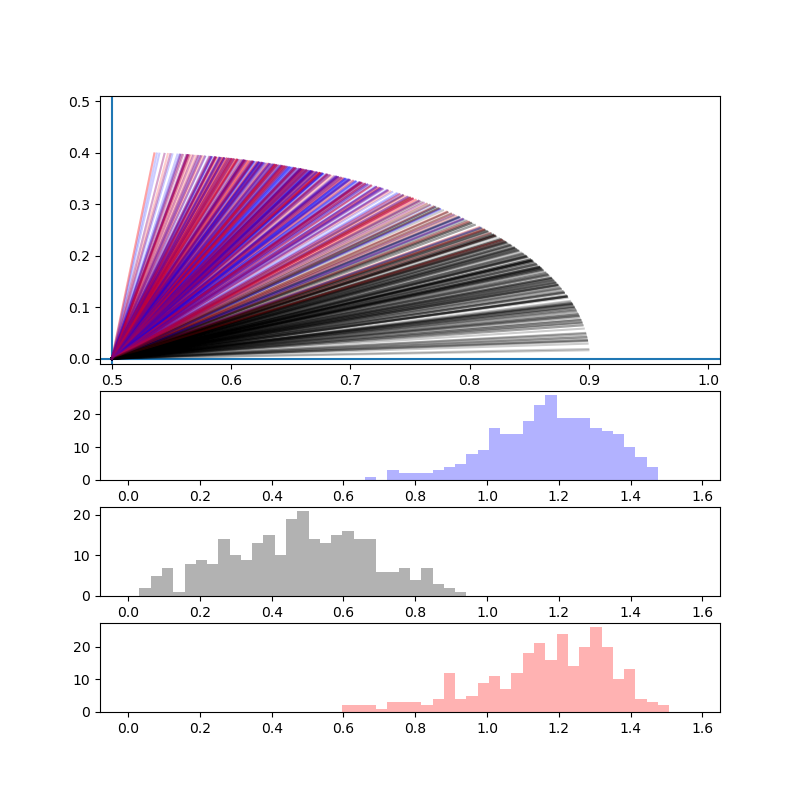
\includegraphics[width=0.50\linewidth, trim=1.5cm 1.5cm 2cm 2cm, clip]{c3_figures/stab-mnist-C32-100-100-10-0.001-200-eval-1e-06-db_interp-angles-1stquadall199.png}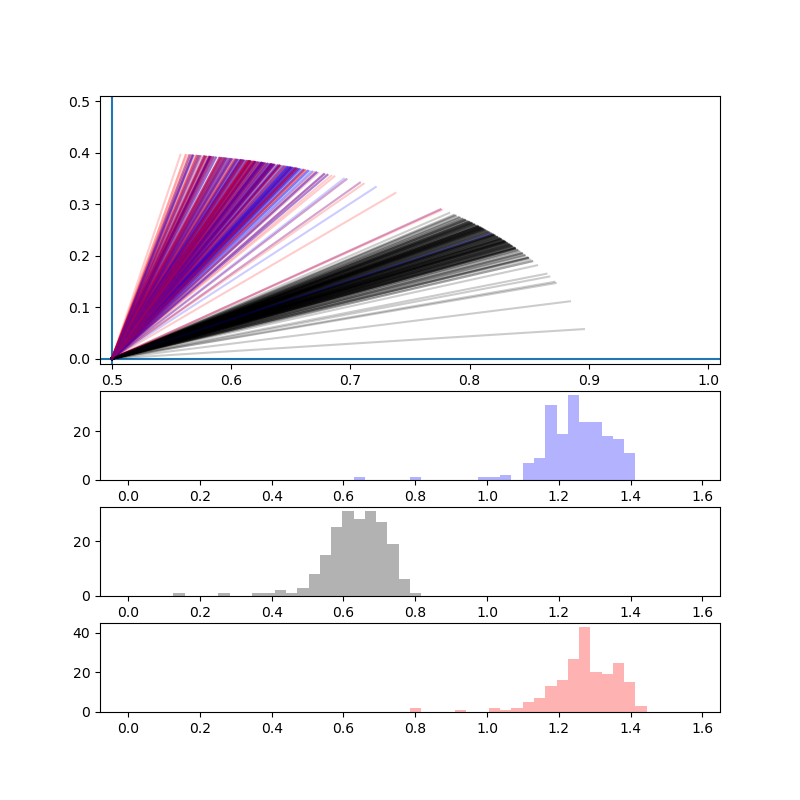
\includegraphics[width=0.50\linewidth, trim=1.5cm 1.5cm 2cm 2cm, clip]{c3_figures/stab-mnist-C32-100-100-10-0.001-200-eval-1e-06-attack-db_interp-angles-1stquadall199.png}

\caption{Decision boundary incident angles between test and test images (left) and between test and adversarial images (right). Angles (plotted Top) are referenced to decision boundary so $\pi/2$ radians (right limit of plots) corresponds with perfect orthogoonality to decision boundary. Lines and histograms measure angles of training gradients (Blue) linear interpolant (Black) and adversarial gradients (Red)}
\label{fig:dba}
\end{figure}

In order to understand this sudden drop in persistence across the decision boundary observed in Figure ~\ref{fig:persistent_interpimage}, we will investigate incident angle of the interpolation with the decision boundary. In order to measure these angles, we must first interpolate along the decision boundary between two points. We will do this for pairs of test and test and pairs of test and adversary. In both cases, we will use a bracketing algorithm along the interpolation from candidate points to identify a point within machine-precision of the decision boundary $x_b$. 

Next, we will take 5000 samples from a Gaussian centered at this point with small standard deviation $\sigma = 10^{-6}$. Next, for each sample, we will perform an adversarial attack in order to produce a corresponding point on the opposite side of the decision boundary. Now for this new pair (sample and attacked sample), we will repeat the interpolation bracketing procedure in order to obtain the projection of this sample onto the decision boundary along the attack trajectory. Next, we will use singular value decomposition (SVD) on the differences between the projected samples and our decision boundary point $x_b$  to compute singular values and vectors from these projected samples. We will use the right singular vector corresponding with the smallest singular value as an approximation of a normal vector to the decision boundary at $x_b$. This point is difficult to compute due to degeneracy of SVD for small singular values, however in our tests, this value could be computed to a precision of 0.003. We will see that this level of precision exceeds exceeds that needed for the angles computed with respect to this normal vector sufficiently. 

From Figure~\ref{fig:dba} we notice that neither training gradients nor adversarial gradients are orthogonal to the decision boundary. From a theory perspective, this is possible because this problem has more than 2 classes, so that the decision boundary includes $(0.34, 0.34, 0.32)$ and $(0.4, 0.4, 0.2)$. That is to say that the level set definition of the decision boundary has degrees of freedom that do not require orthogonality of gradients. More interestingly, both natural and adversarial linear interpolants tend to cross at acute angles with respect to the decision boundary, with adversarial attacks tending to be less acute. This suggests that adversaries are exploiting the obliqueness of the decision boundary with respect to test points. We will leverage this understanding with manifold alignment to see if constraining gradients to a lower dimensional manifold, and thus increasing orthogonality of gradients will increase robustness. 

% \begin{figure}[h]
%     \centering
%     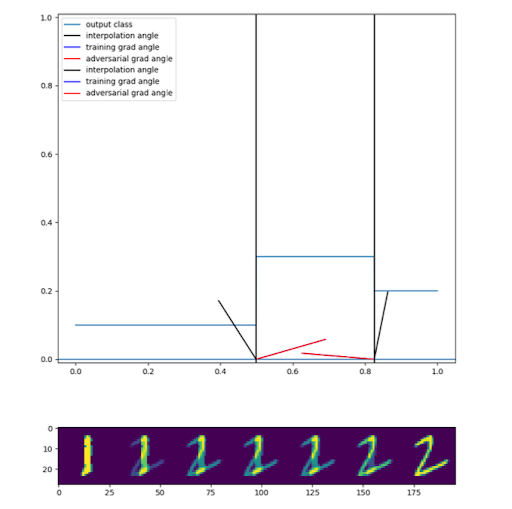
\includegraphics[width=0.8\linewidth]{c2_figures/db_angles_plot.png}
%     \caption{Plot demonstrating the angles at which a linear path interpolation crosses a decision boundary. The output class term is argmaxed, which results in a step functions. Black lines indicate the angle between the interpolation vector and the plane defined by the decision boundary. Crossing askew is a weak support for the dimpled manifold hypothesis presented by \cite{shamir2021dimpled}.}
%     \label{fig:venn}
% \end{figure}


\subsection{Manifold Alignment on MNIST via PCA} \label{subsec:mae}

In order to provide an empirical measure of alignment, we first require a well defined image manifold.
The task of discovering the true structure of \textit{k}-dimensional manifolds in $\mathds{R}^d$ given a set of points sampled on the manifold has been studied previously \citep{khoury2018geometry}.
Many algorithms produce solutions which are provably accurate under data density constraints.
Unfortunately, these algorithms have difficulty extending to domains with large $d$ due to the curse of dimensionality.
Our solution to this fundamental problem is to sidestep it entirely by redefining our dataset.
We begin by projecting our data onto a well known low dimensional manifold, which we can then measure with certainty.
\begin{figure}[h]
\begin{center}
    % \fbox{\rule[-.5cm]{0cm}{4cm} \rule[-.5cm]{4cm}{0cm}}

    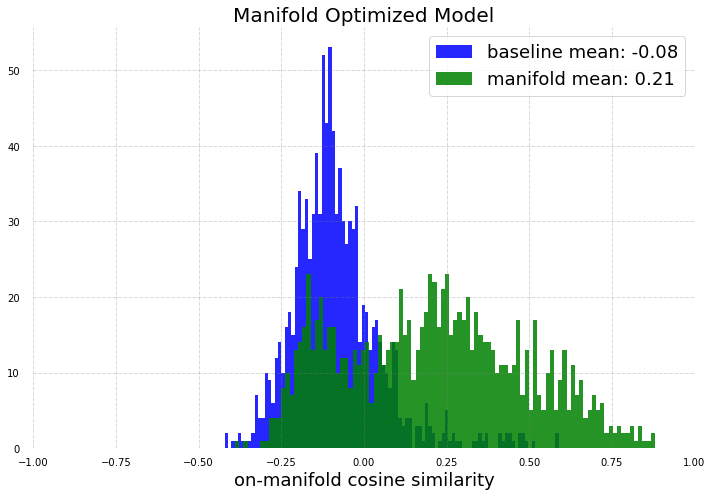
\includegraphics[width=0.8\linewidth]{c3_figures/manifold_model_cosine_hist.png}
    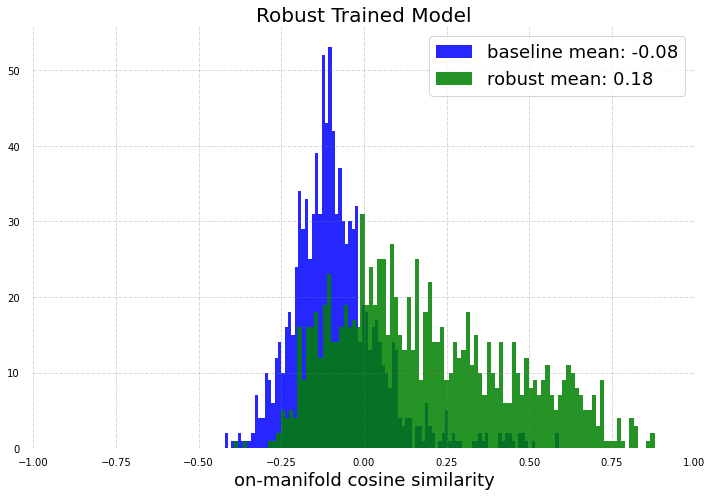
\includegraphics[width=0.8\linewidth]{c3_figures/robust_model_cosine_hist.png}
\end{center}
    \caption{Comparison of on-manifold components between baseline network, robust trained models, and manifold optimized models. Large values indicate higher similarity to the manifold. Both robust and manifold optimized models are more 'on-manifold' than the baseline, with adversarial training being slightly less so.}
    \label{fig:hist_cosine}
\end{figure}




\begin{figure}[h]
    \centering
    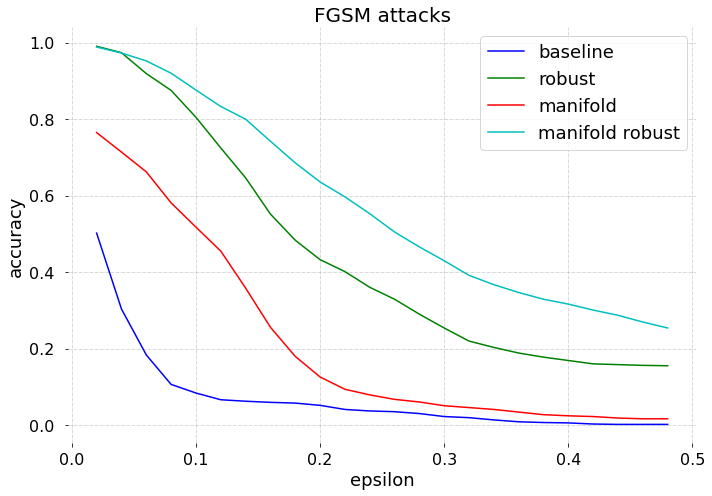
\includegraphics[width=0.8\linewidth]{c3_figures/FGSM_attacks_accuracy_known_manifold.png}
    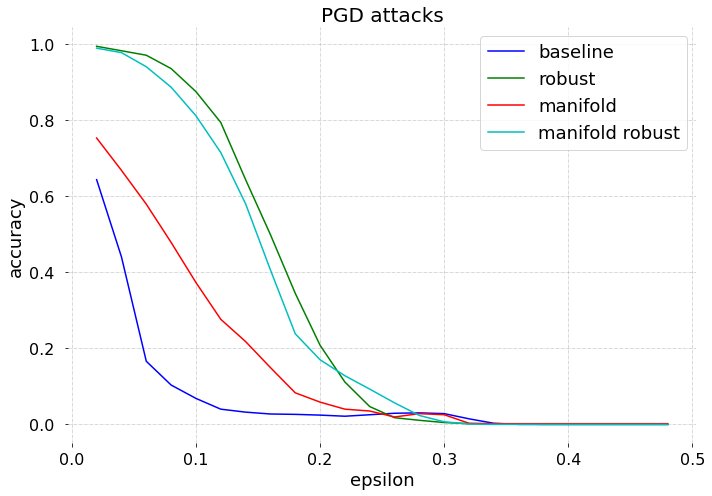
\includegraphics[width=0.8\linewidth]{c3_figures/PGD_attacks_accuracy_known_manifold.png}
    \caption{Comparison of adversarial robustness for PMNIST models under various training conditions. For both FGSM and PGD, we see a slight increase in robustness from using manifold optimization. Adversarial training still improves performance significantly more than manifold optimization. Another observation to note is that when both the manifold, and adversarial objective were optimized, increased robustness against FGSM attacks was observed. All robust models were trained using the $l_\infty$ norm at epsilon = 0.1.}
    \label{fig:model_robustness}
\end{figure}

We first fit a PCA model on all training data, using $k$ components for each class, where $k << d$.
Given the original dataset $X$, we create a new dataset $X_{\mathcal{M}} := \{x \times \textbf{W}^T \times \textbf{W} : x \in X \}$.
We will refer to this set of component vectors as $\textbf{W}$.
Because the rank of the linear transformation matrix, $k$, is defined lower than the dimension of the input space, $d$, this creates a dataset which lies on a linear subspace of $\mathds{R}^d$.
This subspace is defined by the span of $X \times \textbf{W}^T$ and any vector in $\mathds{R}^d$ can be projected onto it.
Any data point drawn from $\{z \times \textbf{W}^T : z \in \mathds{R}^k \}$ is considered a valid datapoint.
This gives us a continuous linear subspace which can be used as a data manifold.

Given that it our goal to study the simplest possible case, we chose MNIST as the dataset to be projected and selected $k = 28$ components.
We refer to this new dataset as Projected MNIST (PMNIST).
The true rank of PMNIST is lower than that of the original MNIST data, meaning there was information lost in this projection.
The remaining information we found is sufficient to achieve 92\% accuracy using a baseline Multylayer Perceptron (MLP), and the resulting images retain their semantic properties as shown in Figure \ref{fig:perception}.

\begin{figure*}
    \centering
    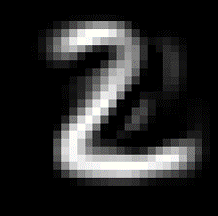
\includegraphics[width=0.25\linewidth]{c3_figures/pag_0.png}
    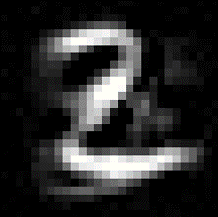
\includegraphics[width=0.25\linewidth]{c3_figures/pag_1.png}
    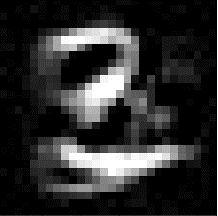
\includegraphics[width=0.25\linewidth]{c3_figures/pag_2.png}
    \caption{Visual example of manifold optimized model transforming 2 into 3. Original PMNIST image on left, center image is center point between original and attacked, on right is the attacked image. Transformation performed using PGD using the $l_\infty$ norm. Visual evidence of manifold alignment is often subjective and difficult to quantify. This example is provided as a baseline to substantiate our claim that our empirical measurements of alignment are valid.}
    \label{fig:perception}
\end{figure*}



Where $L(\theta, x, y)$ represents our classification loss term and $\alpha$ is a hyper parameter determining the weight of the manifold loss term.



% \begin{figure}
% \begin{center}
%     % \fbox{\rule[-.5cm]{0cm}{4cm} \rule[-.5cm]{4cm}{0cm}}

%     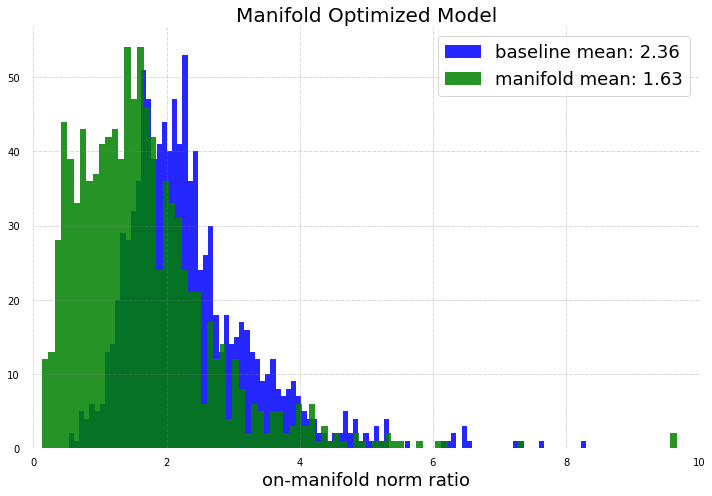
\includegraphics[width=0.8\linewidth]{c3_figures/manifold_model_hist.png}
%     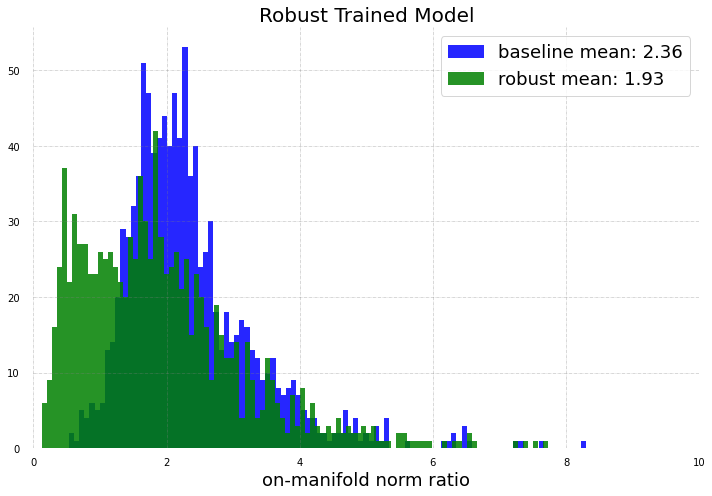
\includegraphics[width=0.8\linewidth]{c3_figures/robust_model_hist.png}
% \end{center}
%     \caption{Comparison of on-manifold components between baseline network, robust trained models, and manifold optimized models. Ratio between a vectors norm and the norm of its projection onto the manifold (Equation \ref{equ:ratio}). Small values indicate higher similarity to the manifold. Both robust and manifold optimized models are more 'on-manifold' than the baseline, with adversarial training being slightly less so. Samples are scaled using $\alpha = 0.1$}
%     \label{fig:hist_ratio}
% \end{figure}


\subsection{Manifold Aligned Gradients} \label{subsec:ma}

% \subsection{Measuring the On-Manifold Component}
Component vectors extracted from the original dataset are used to project gradient examples onto our pre-defined image manifold.
% Given a known manifold, we can project gradients and force our model to learn the structure of this manifold.
% In the case of MNIST we 
Given a gradient example $\nabla_x = \frac{\partial f_\theta(x, y)}{\partial x}$ where $f_\theta$ represents a neural network parameterized by weights $\theta$. $\nabla_x$ is transformed using the coefficient vectors \textbf{W}.
% We define a set of class specific linear transformations using PCA.
\begin{equation}
    \rho_x = \nabla_x \times \textbf{W}^T \times \textbf{W}    
\end{equation}
The projection of the original vector onto this new transformed vector we will refer to as $P_{\mathcal{M}}$.
The norm of this projection gives a metric of manifold alignment.
\begin{equation}
    \frac{|| \nabla_x || }{||P_{\mathcal{M}}(\nabla_x )||}
  \label{equ:ratio}
\end{equation}
This gives us a way of measuring the ratio between on-manifold and off-manifold components of the gradient.
Additionally, both cosine similarity and the vector rejection were also tested but the norm ratio we found to be the most stable in training.
We use this measure as both a metric and a loss, allowing us to optimize the following objective.
\begin{equation}
  \mathds{E}_{(x,y) \sim \mathcal{D}} \left[ L(\theta, x,y)  + \alpha \frac{|| \nabla_x || }{||P_{\mathcal{M}}(\nabla_x )||} \right]
  \label{equ:loss}
\end{equation}


% ----------------------- EXPERIMENTS 
\subsection{Manifold Alignment Robustness Results}

All models were two layer MLPs with 1568 nodes in each hidden layer.
The hidden layer size was chosen as twice the input size.
This arrangement was chosen to maintain the simplest possible case.

Two types of attacks were leveraged in this study: fast gradient sign method (FGSM) \citep{goodfellow_explaining_2014} and projected gradient descent (PGD) \citep{madry_towards_2017}.
A total of four models were trained and evaluated on these attacks: Baseline, Robust, Manifold and Manifold Robust.
All models, including the baseline, were trained on PMNIST.
``Robust" in our case refers to adversarial training.
All robust models were trained using the $l_\infty$ norm at $\epsilon = 0.1$.
Manifold Robust refers to both optimizing our manifold objective and robust training simultaneously.

Figure \ref{fig:hist_cosine} shows the cosine similarity on the testing set of PMNIST for both the Manifold model and Robust model.
Higher values indicate the model is more aligned with the manifold.
Both models here are shown to be more on manifold than the Baseline.
This demonstrates that our metric for alignment is being optimized as a consequence of adversarial training.

Figure \ref{fig:model_robustness} shows the adversarial robustness of each model.
In both cases, aligning the model to the manifold shows an increase in robustness over the baseline.
However, we do not consider the performance boost against PGD to be significant enough to call these models robust against PGD attacks.
Another point of interest that while using both our manifold alignment metric and adversarial training, we see an even greater improvement against FGSM attacks.
% This demonstrates that the gain in robustness learned by our metric is distinct from the performance gained by FGSM training.
The fact that this performance increase is not shared by PGD training may indicate a relationship between these methods.
Our current hypothesis is that a linear representation of the image manifold is sufficient to defend against linear attacks such as FGSM, but cannot defend against a non-linear adversary.


\section{Conclusion}

%In general, our intuition that adversarial examples are less stable than than natural examples is supported by the results in Table \ref{table1}. 


%The more complex neural networks tended to support less stable adversarial examples, but ones that are closer to the natural examples. 


In order to better understand the observed tendency for points near natural data to be classified similarly and points near
adversarial examples to be classified differently, we defined a notion of $(\gamma,\sigma)$-stability which is easily estimated by Monte Carlo sampling. For any data point $x$, we then define the $\gamma$-persistence to to be the smallest $\sigma_\gamma$ such that the probability of similarly classified data is at least $\gamma$ when sampling from Gaussian distributions with mean $x$ and standard deviation less than $\sigma_\gamma$. The persistence value can be quickly estimated by a Bracketing Algorithm. These two measures were considered with regard to both the MNIST and ImageNet datasets and with respect to a variety of classifiers and adversarial attacks. We found that adversarial examples were much less stable than natural examples in that the $0.7$-persistence for natural data was usually significantly larger than the $0.7$-persistence for adversarial examples. We also saw that the dropoff of the persistence tends to happen precisely near the decision boundary. Each of these observations is strong evidence toward the hypothesis that adversarial examples exploit oblique structure of overlapping decision boundaries around the adversarial class, whereas natural images lie outside such regions.In addition, we found that some adversarial examples may be more stable than others, and a more detailed probing using the concept of $(\gamma,\sigma)$-stability and the $\gamma$-persistence statistic may be able to help with a more nuanced understanding of the geometry and obliqueness of the boundary.

We reinforced this obliqueness hypothesis by computing angles of linear interpolants with respect to the decision boundary, showing that most interpolants cross the decision boundary between classes at very shallow angles. Furthermore, adversarial interpolants tend to cross at less shallow, but still acute angles. Furthermore, we present the simplest possible case of our hypothesis that manifold alignment implies adversarial robustness.
Extending this to show results on more complex models and datasets is left to future work.
In this early work, we only test against a linear manifold and show that it provides robustness against FGSM.
We conclude that training a model to be aligned with a low dimensional manifold on which your data lies is related to robust training.
While this model shows some properties of adversarial robustness, it is still vulnerable to PGD attacks.
Additionally, a model trained to be robust using adversarial training shows manifold alignment under our definition.

%We also found that often the most likely class for perturbations of an adversarial examples is a class other than the class of the original natural example used to generate the adversarial example; instead, some other background class is favored. 
%In addition, we found that some adversarial examples may be more stable than others, and a more detailed probing using the concept of $(\gamma,\sigma)$-stability and the $\gamma$-persistence statistic may be able to help with a more nuanced understanding of the geometry and obliqueness of the boundary. %Although not pursued here, the observations and statistics used in this paper could potentially be used to develop methods to detect adversarial examples as in \cite{crecchi2019,frosst2018,hosseini2019odds,Lee2018ASU,qin2020,roth19aodds} and others. As with other methods of detection, this may be susceptible to adaptive attacks as discussed by \citet{tramer2020adaptive}. 







% Acknowledgements should only appear in the accepted version.
% \section*{Acknowledgements}



% In the unusual situation where you want a paper to appear in the
% references without citing it in the main text, use \nocite
\nocite{langley00}





% %%%%%%%%%%%%%%%%%%%%%%%%%%%%%%%%%%%%%%%%%%%%%%%%%%%%%%%%%%%%

% \newpage
% \appendix

% \section{Bracketing Algorithm}\label{sec:bracketing}
% The Bracketing Algorithm is a way to determine persistance of an image with respect to a given classifier, typically a DNN. The algorithm was implemented in Python for the experiments presented. The \textproc{rangefinder} function is not strictly necessary, in that one could directly specify values of $\sigma_{\min}$ and $\sigma_{\max}$, but we include it here so that the code could be automated by a user if so desired.  

% % \begin{algorithm} [h!]
% % \begin{algorithmic}
% % \Function{bracketing}{image, DNN, numSamples, $\gamma$, maxSteps, precision}
% %  \Comment{ start with same magnitude noise as image}
% %  \State u\_tol, l\_tol = 1+ precision, 1-precision
% %  \State a\_var = Variance(image)/4 \Comment{Running Variance}
% %  \State l\_var, u\_var  = 0, a\_var*2\Comment{ Upper and Lower
% %   Variance of search space}
% %  \Comment{ Adversarial image plus noise counts}
% %  \State a\_counts = zeros(n)
% %  \State n\_sz = image.shape[0]
% %  \State mean = Zeros(n\_sz)
% %  \State I = Identity(n\_sz)
% %  \State count = 0
% % \Comment{grab the classification of the image under the network}
% % \State y\_a = argmax(DNN.forward(image))
% % \State samp = N(0, u\_var*I, numSamples)
% % \State image\_as = argmax(DNN.forward(image + samp))
% % \Comment{Expand search window}
% % \While{Sum(image\_as == y\_a) $>$ numSamples*$\gamma$/2} \Comment{Gaussian sampling}
% % \State u\_var = u\_var*2
% % \State samp = N(0, u\_var*I, numSamples)
% % \State image\_as = argmax(DNN.forward(image + samp))
% % \EndWhile
% %   \Comment{ perform the bracketing }
% % \For{i in range(1,maxSteps)}
% % \State count+=1
% % \Comment{compute sample and its torch tensor}
% % \State samp = N(0, a\_var*I, numSamples)

% % \State image\_as = argmax(DNN.forward(image + samp))

% % \State a\_counts[i] = Sum(image\_as == y\_a)

% % \Comment{floor and ceiling surround number}
% % \If{((a\_counts[i] $\leq$ Ceil(numSamples*($\gamma$*u\_tol))) \& (a\_counts[i] $>$ Floor(numSamples*($\gamma$*l\_tol))))}

% %         \Return{a\_var}
% %     \ElsIf{ (a\_counts[i] $<$ numSamples*$\gamma$)} \Comment{we're too high}
% %         \State u\_var = a\_var
% %         \State a\_var = (a\_var + l\_var)/2
% %     \ElsIf{ (a\_counts[i] $\geq$ numSamples*$\gamma$)} \Comment{we're too low}
% %         \State l\_var = a\_var
% %         \State a\_var = (u\_var + a\_var)/2
% %         \EndIf
% % \EndFor

% %   \Return{a\_var}
% % \EndFunction
% % \end{algorithmic}
% % \caption{Bracketing algorithm for computing $\gamma$-persistence}\label{bracketing}
% % \end{algorithm}



% \begin{algorithm} [h!]
% \begin{algorithmic}
% \Function{bracketing}{image, classifier ($\CC$), numSamples, $\gamma$, maxSteps, precision}

% \State $[\sigma_{\min},\sigma_{\max}] = $\textproc{rangefinder}(image, $\CC$, numSamples, $\gamma$)
% \State count $=1$
% \While{count$<$maxSteps}
% \State $\sigma = \frac{\sigma_{\min}+\sigma_{\max}}{2}$
% \State $\gamma_{\textnormal{new}} =$ \textproc{compute\_persistence}($\sigma$, image, numSamples, $\CC$)
% \If{$|\gamma_{\textnormal{new}}-\gamma|<$precision}
% \State \textbf{return} $\sigma$ %$\gamma_{\textnormal{new}}$
% \ElsIf{$\gamma_{\textnormal{new}}>\gamma$}
% \State $\sigma_{\min} = \sigma$
% \Else
% \State $\sigma_{\max} = \sigma$
% \EndIf
% \State count = count + 1
% \EndWhile

% \Return $\sigma$
% \EndFunction

% \\
% \Function{rangefinder}{image, $\CC$, numSamples, $\gamma$}
% \State $\sigma_{\min}=.5$,\;\; $\sigma_{\max}=1.5$
% \State $\gamma_1 =$ \textproc{compute\_persistence}($\sigma_{\min}$, image, numSamples, $\CC$)
% \State $\gamma_2 =$ \textproc{compute\_persistence}($\sigma_{\max}$, image, numSamples, $\CC$)
% \While{$\gamma_1<\gamma$ \textbf{or} $\gamma_2>\gamma$}
% \If{$\gamma_1<\gamma$}
% \State $\sigma_{\min} = .5\sigma_{\min}$
% \State $\gamma_1 =$ \textproc{compute\_persistence}($\sigma_{\min}$, image, numSamples, $\CC$)
% \EndIf
% \If{$\gamma_2>\gamma$}
% \State $\sigma_{\max} = 2\sigma_{\max}$
% \State $\gamma_2 =$ \textproc{compute\_persistence}($\sigma_{\max}$, image, numSamples, $\CC$)
% \EndIf
% \EndWhile

% \Return{$[\sigma_{\min}, \sigma_{\max}]$}
% %\sigma_{\min},\sigma_{\max}$}
% \EndFunction

% \\
% \Function{compute\_persistence}{$\sigma$, image, numSamples, $\CC$}
% \State sample = $N(\textnormal{image},\sigma^2I,$numSamples)
% \State $\gamma_{\textnormal{est}} = \frac{|\{\CC(\textnormal{sample})=\CC(\textnormal{image})\}|}{\textnormal{numSamples}}$

% \Return{$\gamma_{\textnormal{est}}$}
% \EndFunction
% \end{algorithmic}
% \caption{Bracketing algorithm for computing $\gamma$-persistence}\label{bracketing}
% \end{algorithm}


% \section{Convolutional neural networks used} \label{appendix:CNNs}
% In Table \ref{table1} we reported results on varying complexity convolutional neural networks. These networks consist of a composition of convolutional layers followed by a maxpool and fully connected layers. 
% The details of the network layers are described in Table \ref{tab:CNN} where Ch is the number of channels in the convolutional components. %\todo{[DG]: We need to simplify to the tables without the truncation}

% %\vspace{.4cm}
% \begin{table}[pt]
% \centering
% \caption{Structure of the CNNs C-Ch used in Table \ref{table1}}
% \label{tab:CNN}
% \begin{tabular}{llllll}
% \toprule
%      Layer & Type & Channels & Kernel & Stride & Output Shape \\
% \midrule
%      0 & Image & 1 & NA & NA & $(1, 28, 28)$ \\
%      1 & Conv & Ch & $(5,5)$& $(1,1)$& $(\textnormal{Ch}, 24, 24)$\\
%      2 & Conv & Ch & $(5,5)$& $(1,1)$& $(\textnormal{Ch}, 20, 20)$\\
%      3 & Conv & Ch & $(5,5)$& $(1,1)$& $(\textnormal{Ch}, 16, 16)$\\
%      4 & Conv & Ch & $(5,5)$& $(1,1)$& $(\textnormal{Ch}, 12, 12)$\\
%      5 & Max Pool & Ch & $(2, 2)$ & $(2, 2)$& $(\textnormal{Ch}, 6, 6)$ \\
%      %6 & Trunc & 1 & NA & NA & $Ch$ \\
%      7 & FC & $(\textnormal{Ch}\cdot 6 \cdot 6, 256)$ & NA & NA & 256 \\
%      8 & FC & $(256, 10)$ & NA & NA & 10 \\
%      \bottomrule
% \end{tabular}
% \end{table}
 
% %[DG: What changes if the number of channels changes? Can we give a general form.]
% %We denote such a network as ``C-Ch-$k$,'' where C reflects that this is a convolutional DNN, Ch denotes the number of channels and $k$ denotes the width of the smallest level, for instance, ``C-128-2''.

% \section{Additional Figures}
% In this section we provide additional figures to demonstrate some of the experiments from the paper.

% %\subsection{Figures interpolating between natural and adversarial examples}
% %In this section we further investigate what happens on the straight line from a natural example to an adversarial example.

% \subsection{Additional figures from MNIST}
% In Figure \ref{fig:mnistadv} we begin with an image of a \texttt{1} and generate adversarial examples to the networks described in Section \ref{sec:mnist} via IGSM targeted at each class \texttt{2} through \texttt{9}; plotted are the counts of output classifications by the DNN from samples from Gaussian distributions with increasing standard deviation; this complements Figure \ref{fgsmo} in the main text. Note that the prevalence of the adversarial class falls off quickly in all cases, though the rate is different for different choices of target class.
% \begin{figure}[!htb]
%     \centering
%     \includegraphics[width=.49\textwidth]{c3_figures/MNISTA2O1.pdf}
%     \includegraphics[width=.49\textwidth]{c3_figures/MNISTA3O1.pdf}
%     \includegraphics[width=.49\textwidth]{c3_figures/MNISTA4O1.pdf}
%     \includegraphics[width=.49\textwidth]{c3_figures/MNISTA5O1.pdf}
%     \includegraphics[width=.49\textwidth]{c3_figures/MNISTA6O1.pdf}
%     \includegraphics[width=.49\textwidth]{c3_figures/MNISTA7O1.pdf}
%     \includegraphics[width=.49\textwidth]{c3_figures/MNISTA8O1.pdf}
%     \includegraphics[width=.49\textwidth]{c3_figures/MNISTA9O1.pdf}
%     \caption{Frequency of each class in Gaussian samples with increasing standard deviations around adversarial attacks of an image of a \texttt{1} targeted at classes \texttt{2} through \texttt{9} on a DNN classifier generated using IGSM. The adversarial class is shown as a red curve. The natural image class (\texttt{1}) is shown in black. Bottoms show example sample images at different standard deviations.}
%     \label{fig:mnistadv}
% \end{figure}

% We also show histograms corresponding to those in Figure \ref{fig:IGSMpersistenceMNIST} and the networks from Table \ref{table1}.  As before, for each image, we used IGSM to generate 9 adversarial examples (one for each target class) yielding a total of 1800 adversarial examples. In addition, we randomly sampled 1800 natural MNIST images. For each of the 3600 images, we computed $0.7$-persistence. In Figure \ref{fig:FC10}, we see histograms of these persistences for the small fully connected networks with increasing levels of regularization. In each case, the test accuracy is relatively low and distortion relatively high. It should be noted that these high-distortion attacks against models with few effective parameters were inherently very stable -- resulting in most of the ``adversarial'' images in these sets having higher persistence than natural images. This suggests a lack of the sharp conical regions which appear to characterize adversarial examples generated against more complicated models.  In Figure \ref{fig:FC100200} we see the larger fully connected networks from Table \ref{table1} and in Figure \ref{fig:CNNs} we see some of the convolutional neural networks from Table \ref{table1}. 

% \begin{figure}[!htb]
% \centering
% 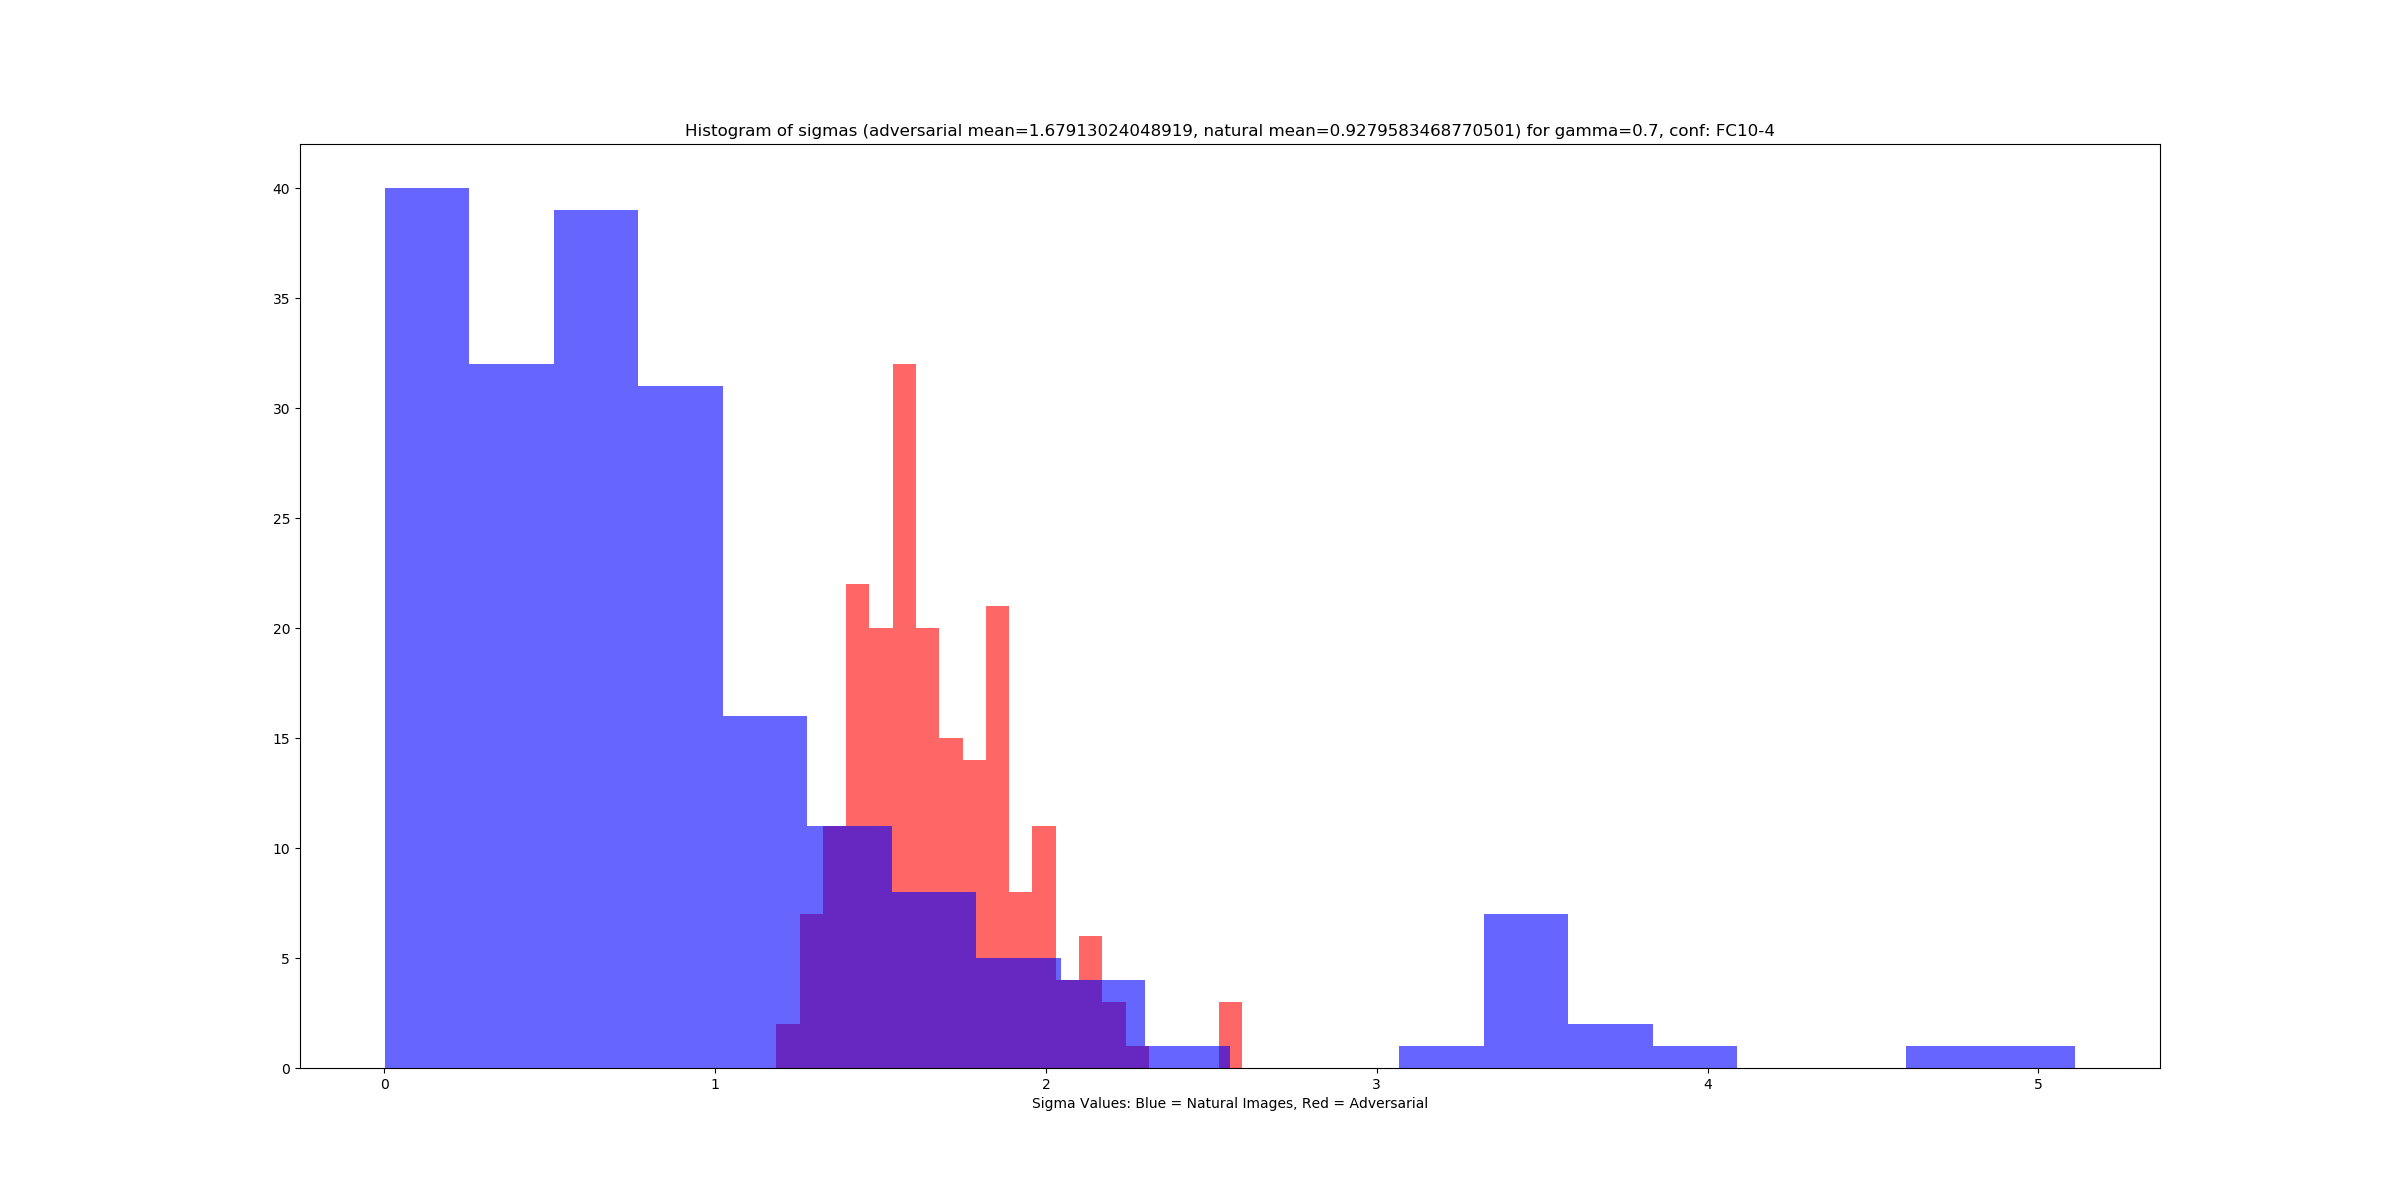
\includegraphics[trim=200 80 100 100, clip,width=.32\textwidth]{c3_figures/gamma_sigma/FC10-4-gamma1_hist.png}
% 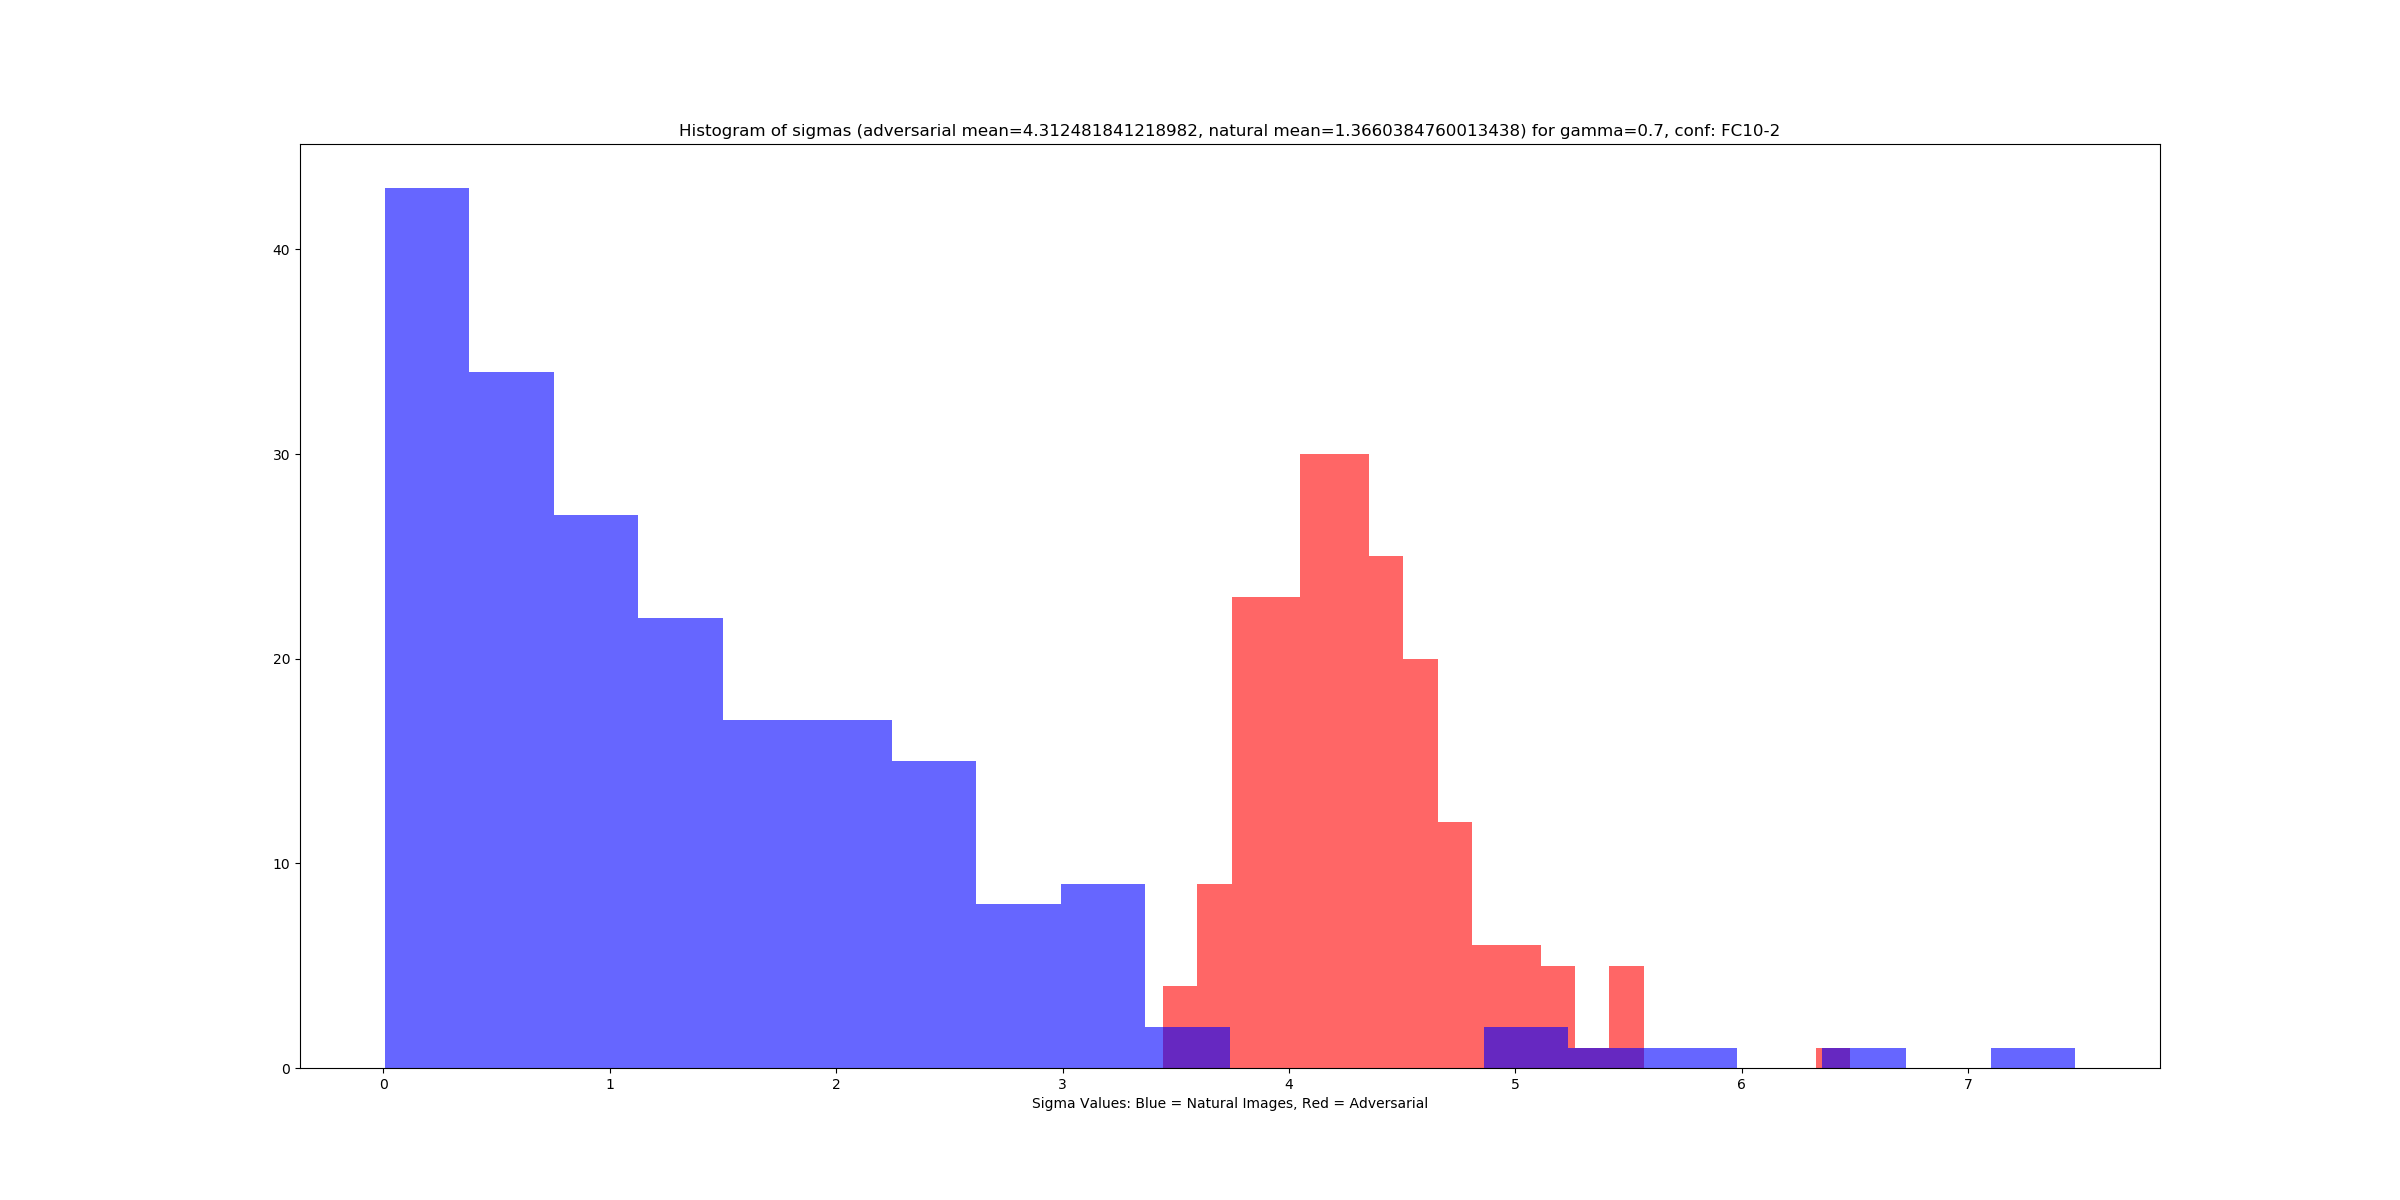
\includegraphics[trim=200 80 100 100, clip,width=.32\textwidth]{c3_figures/gamma_sigma/FC10-2-gamma1_hist.png}
% 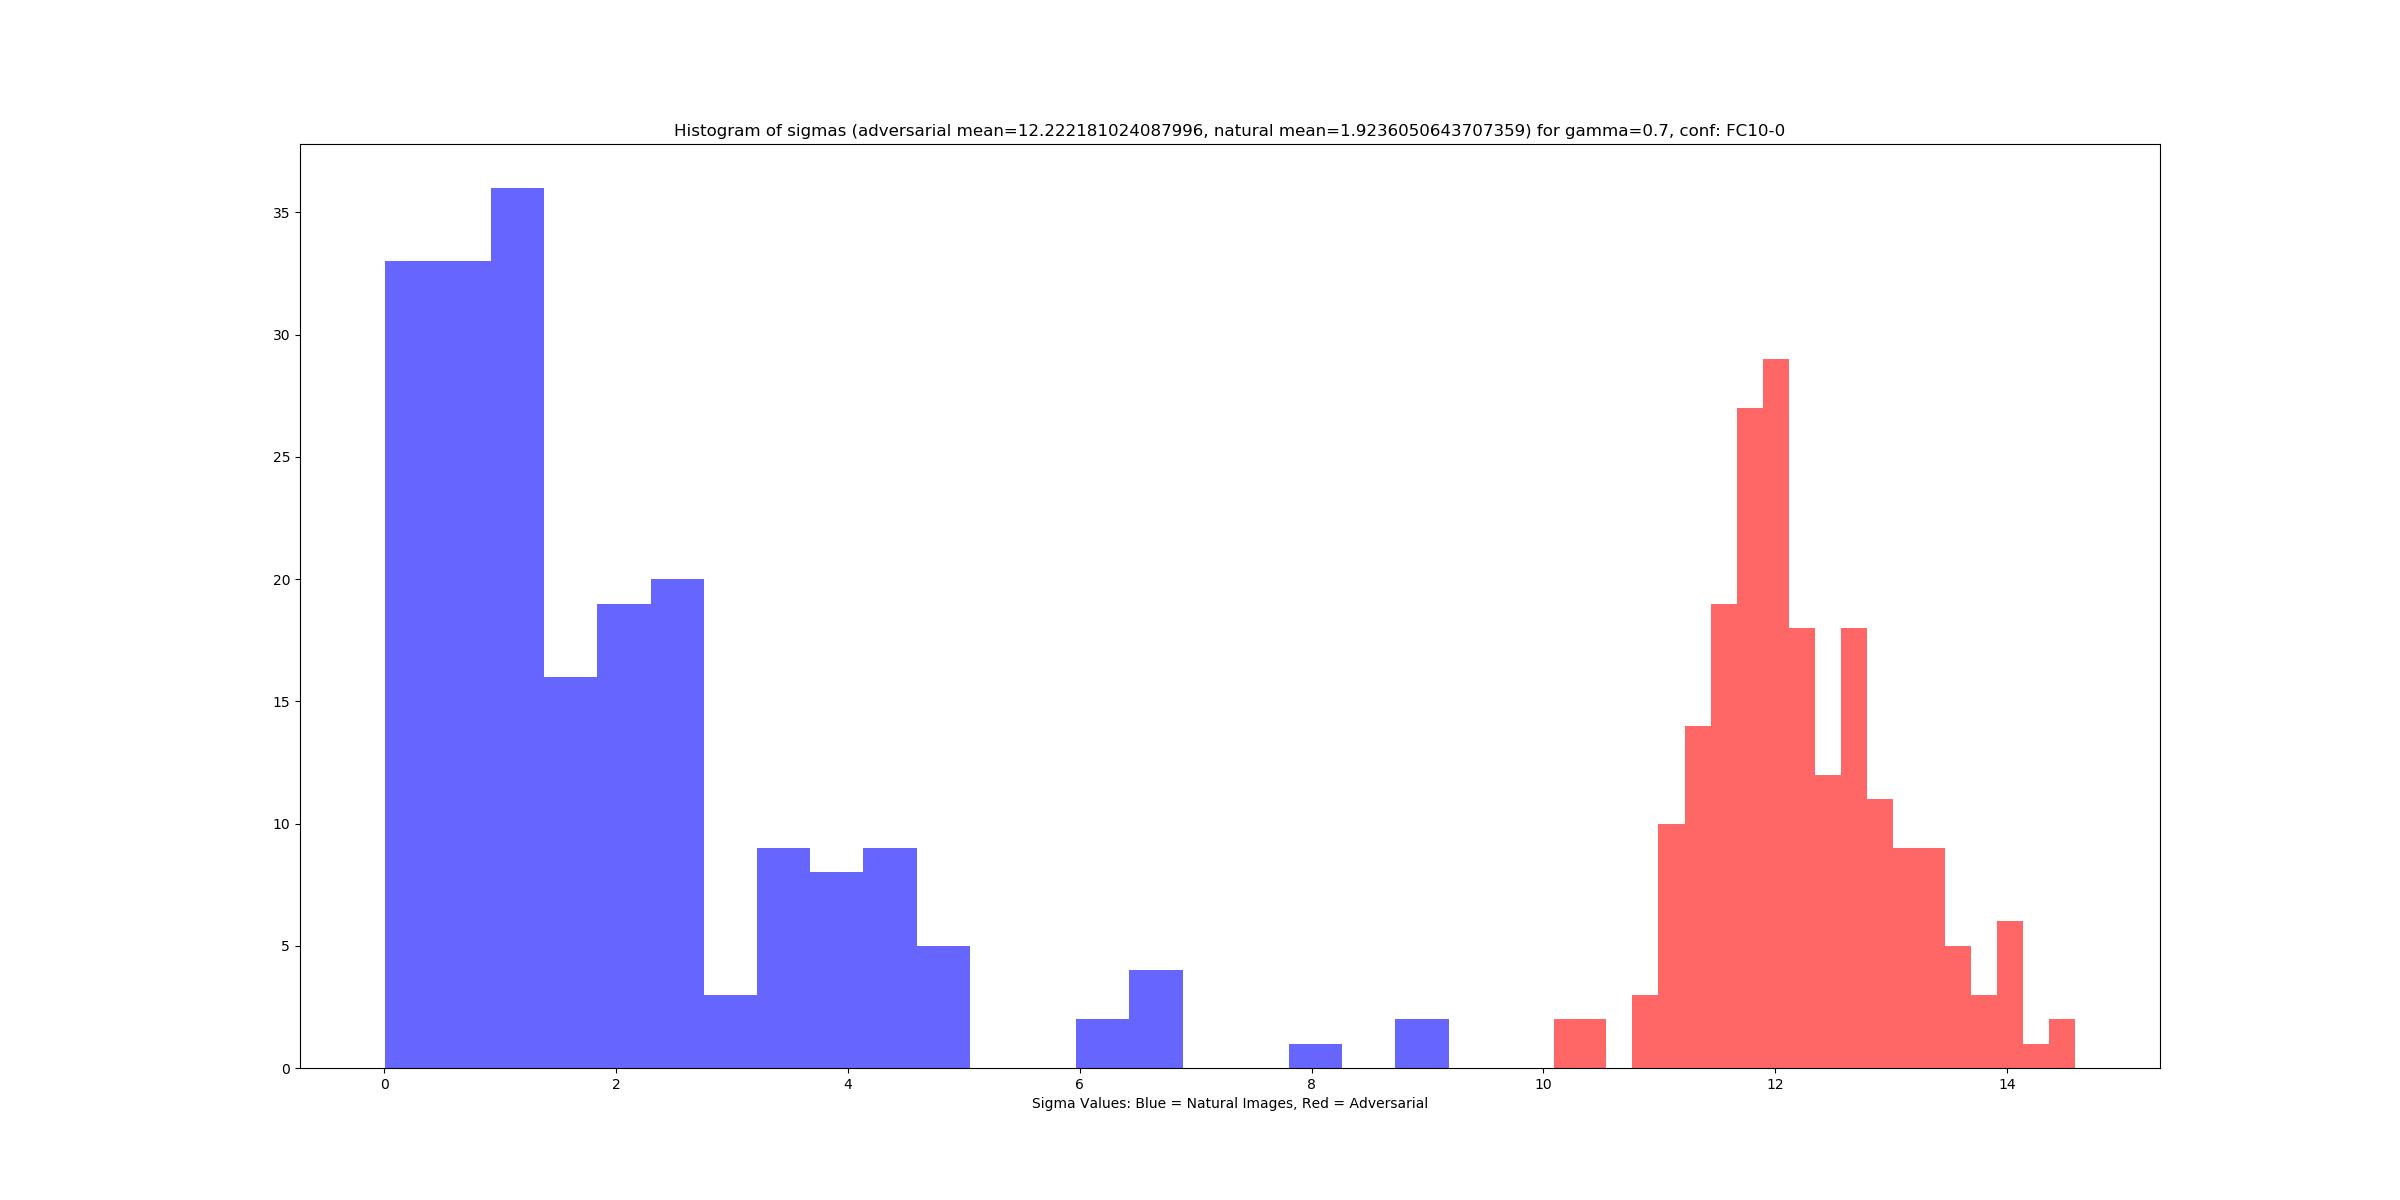
\includegraphics[trim=200 80 100 100, clip,width=.32\textwidth]{c3_figures/gamma_sigma/FC10-0-gamma1_hist.png}
% \caption{Histograms of $0.7$-persistence for FC10-4 (smallest regularization, left), FC10-2 (middle), and FC10-0 (most regularization, right) from Table \ref{table1}. Natural images are in blue, and adversarial images are in red. Note that these are plotted on different scales -- higher regularization forces any "adversaries" to be very stable.\vspace{2em} }
% \label{fig:FC10}
% \end{figure}

% \begin{figure}[!htb]
% \centering
% 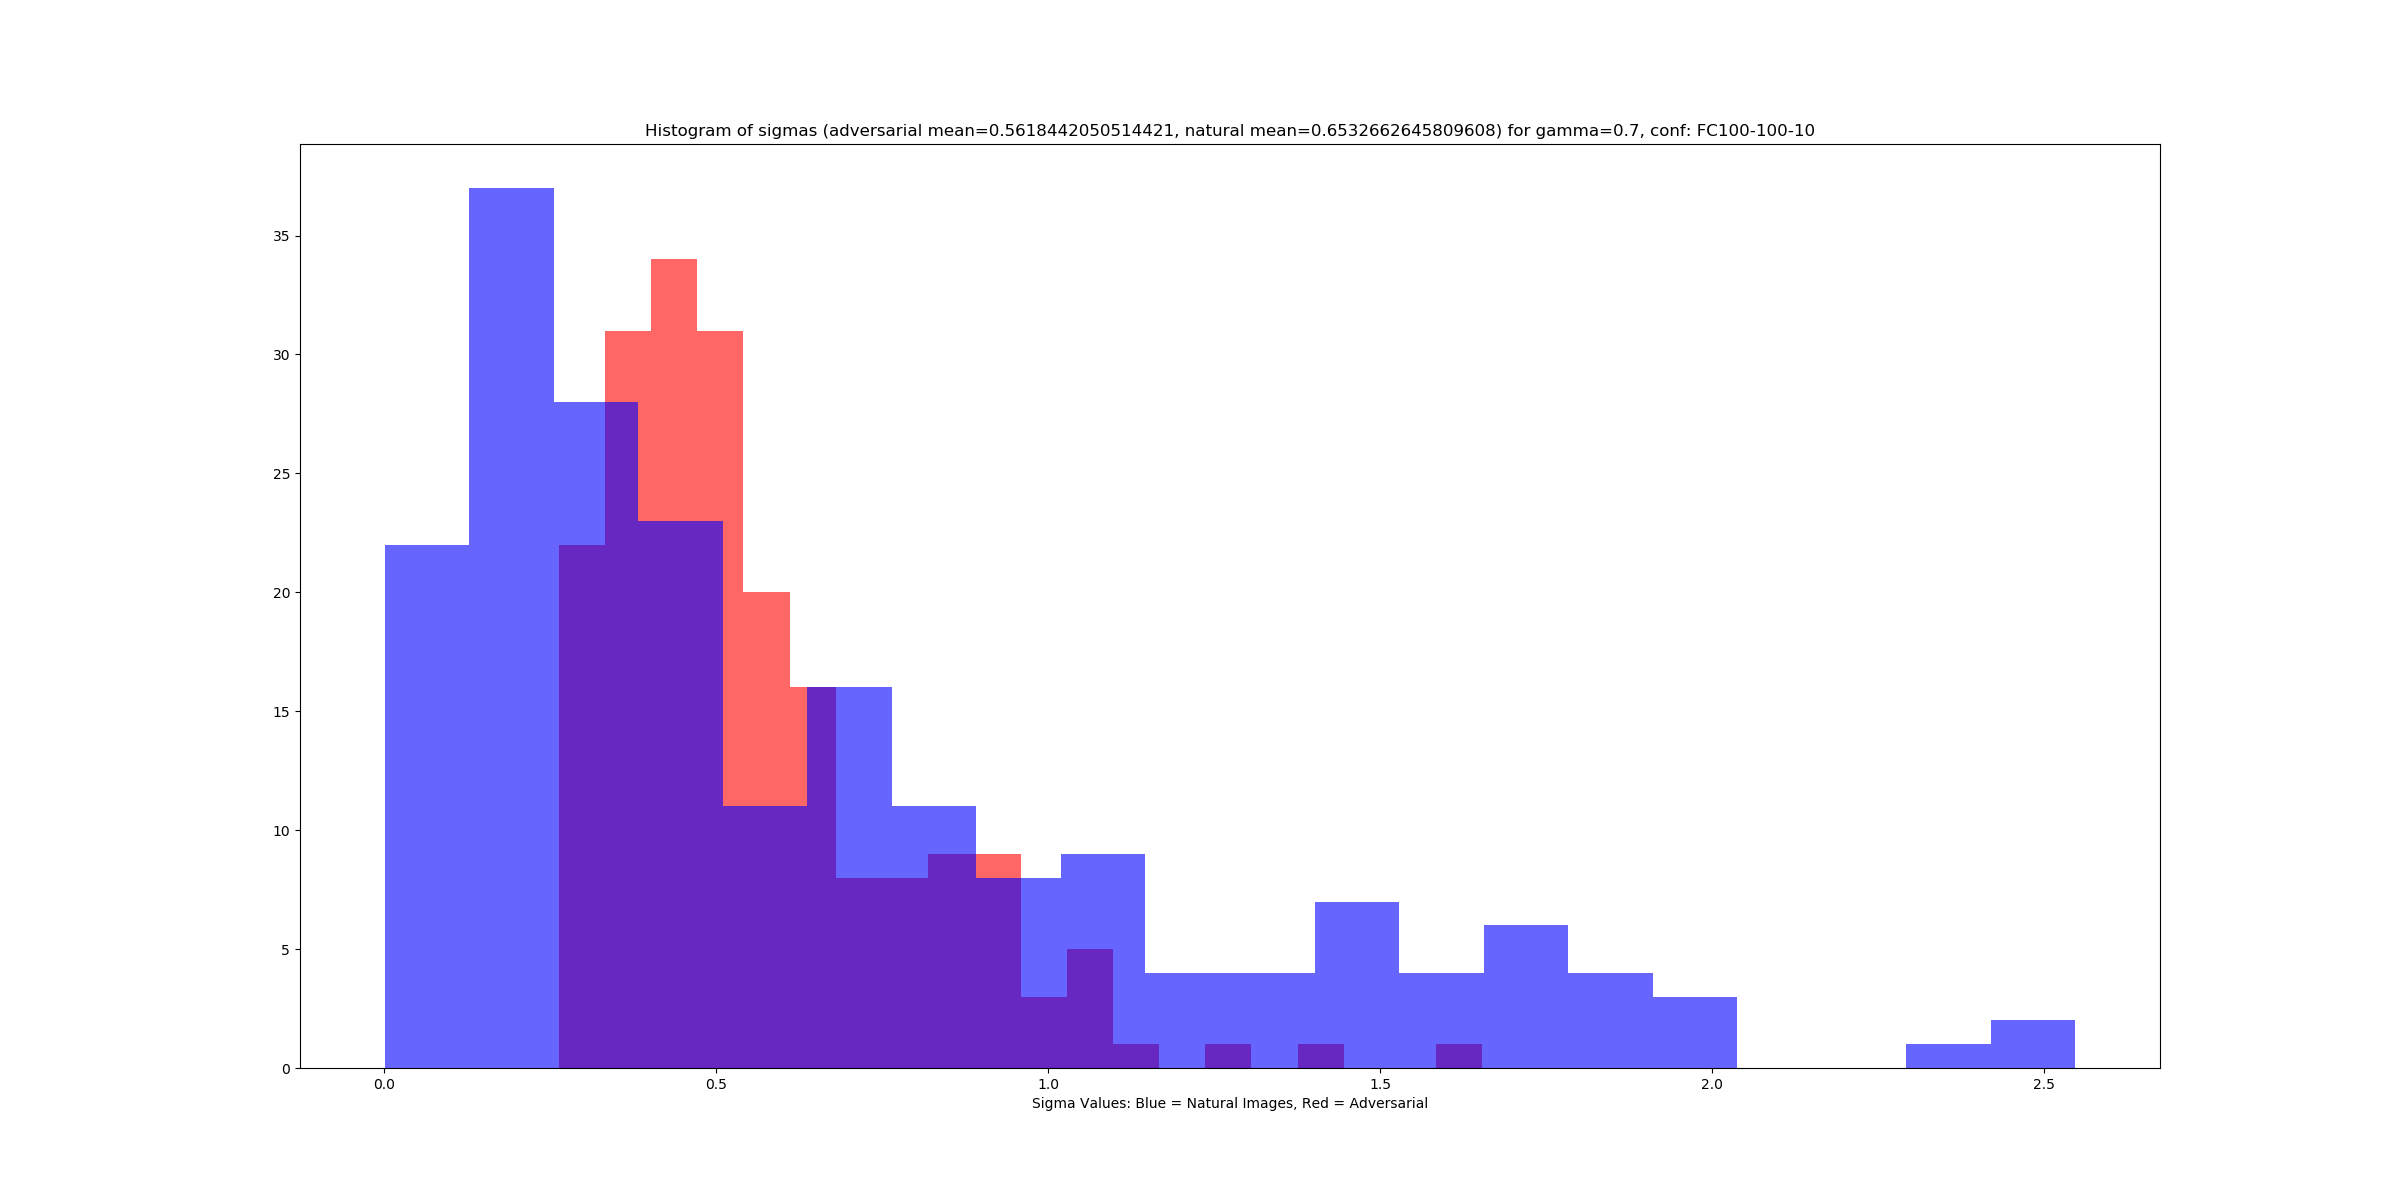
\includegraphics[trim=200 80 100 100, clip,width=.49\textwidth]{c3_figures/gamma_sigma/FC100-100-10-gamma1_hist.png}
% 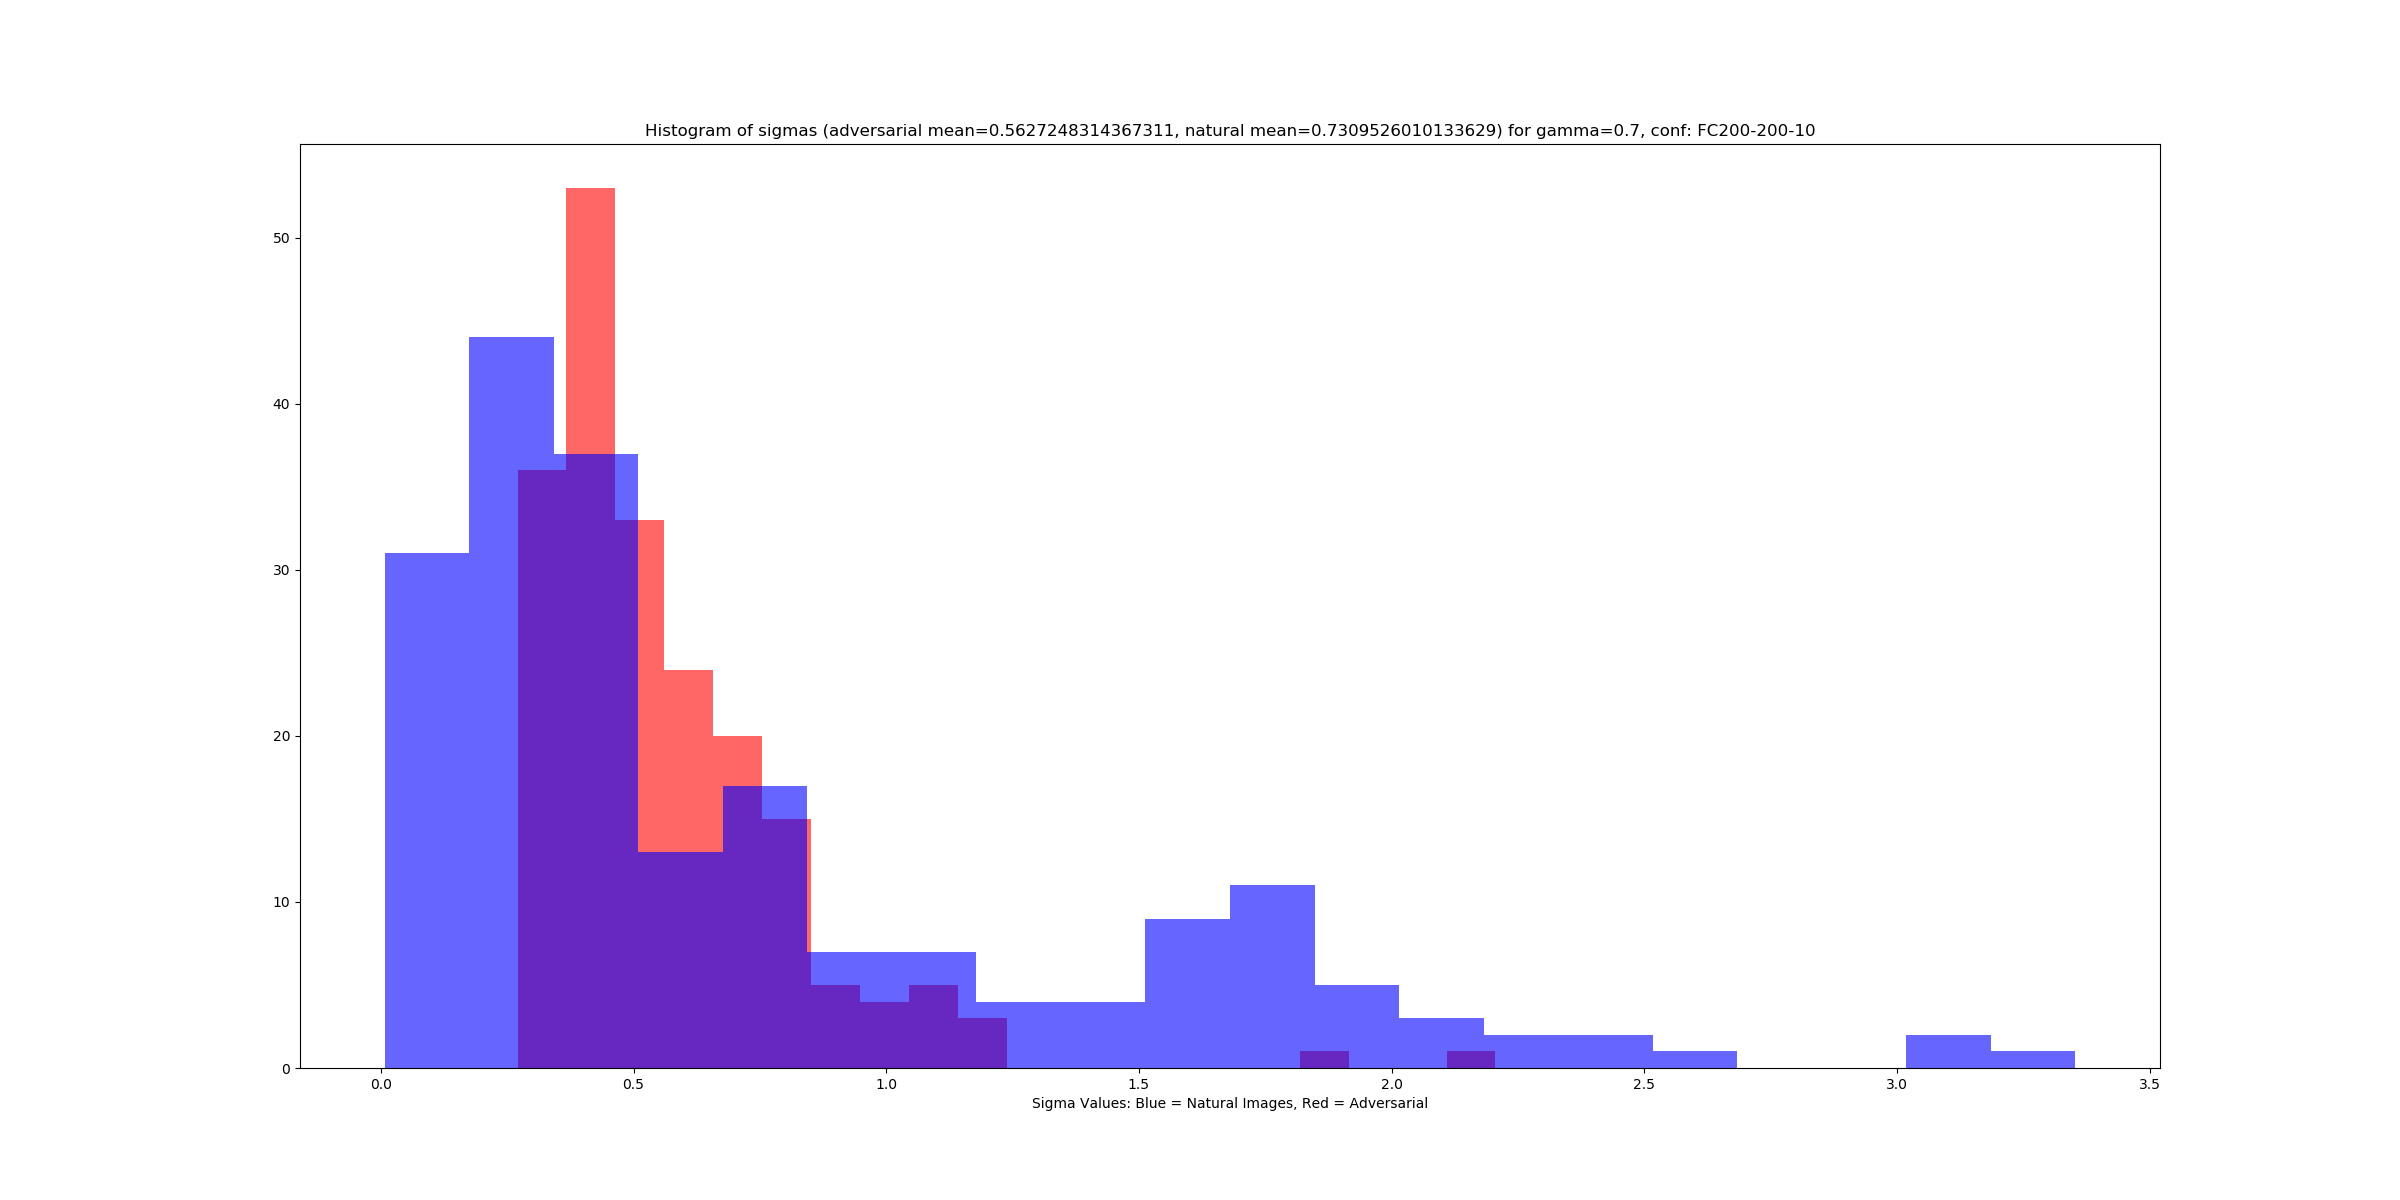
\includegraphics[trim=200 80 100 100, clip,width=.49\textwidth]{c3_figures/gamma_sigma/FC200-200-10-gamma1_hist.png}
% \caption{Histograms of $0.7$-persistence for FC100-100-10 (left) and FC200-200-10 (right) from Table \ref{table1}. Natural images are in blue, and adversarial images are in red.}
% \label{fig:FC100200}
% \end{figure}

% \begin{figure}[!htb]
% 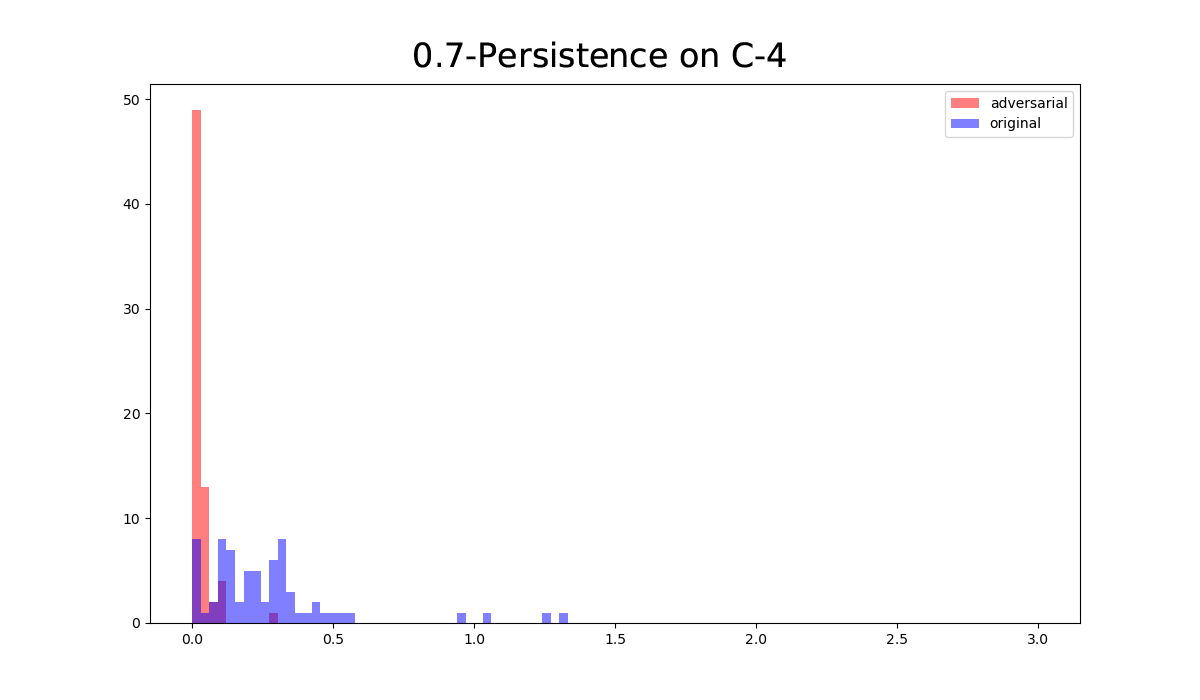
\includegraphics[width=.49\textwidth]{c3_figures/MNIST-C-4-0-stab_compare_a_var-hist.png}
% 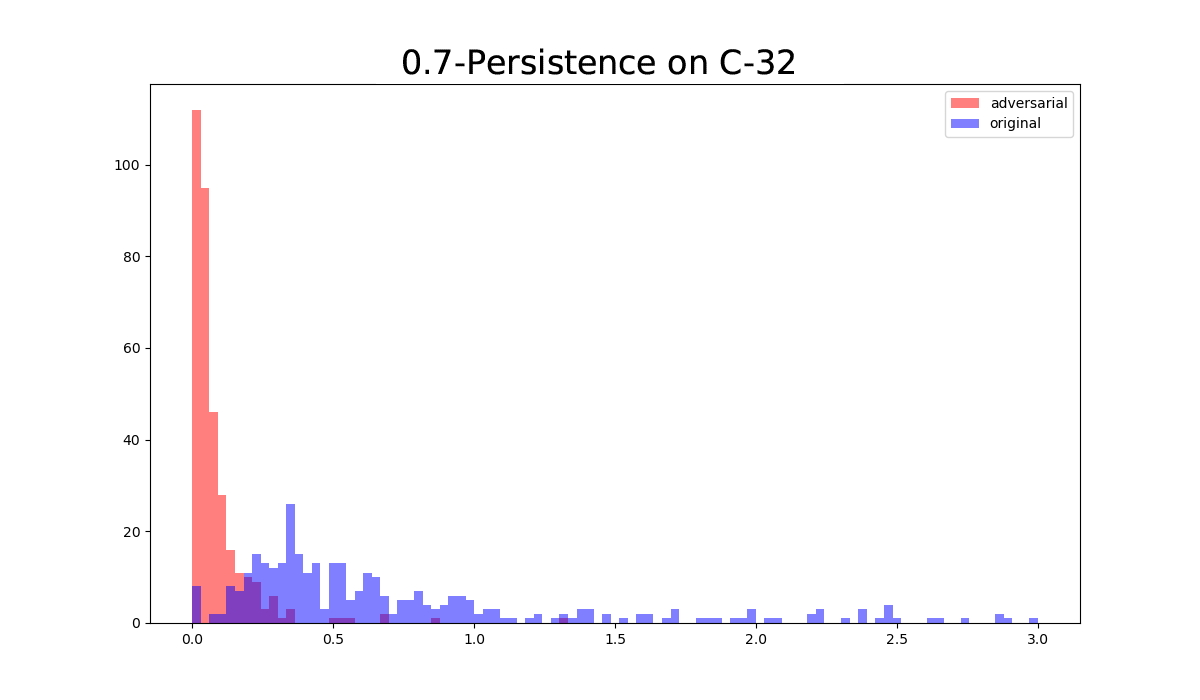
\includegraphics[width=.49\textwidth]{c3_figures/MNIST-C-32-0-stab_compare_a_var-hist.png}
% 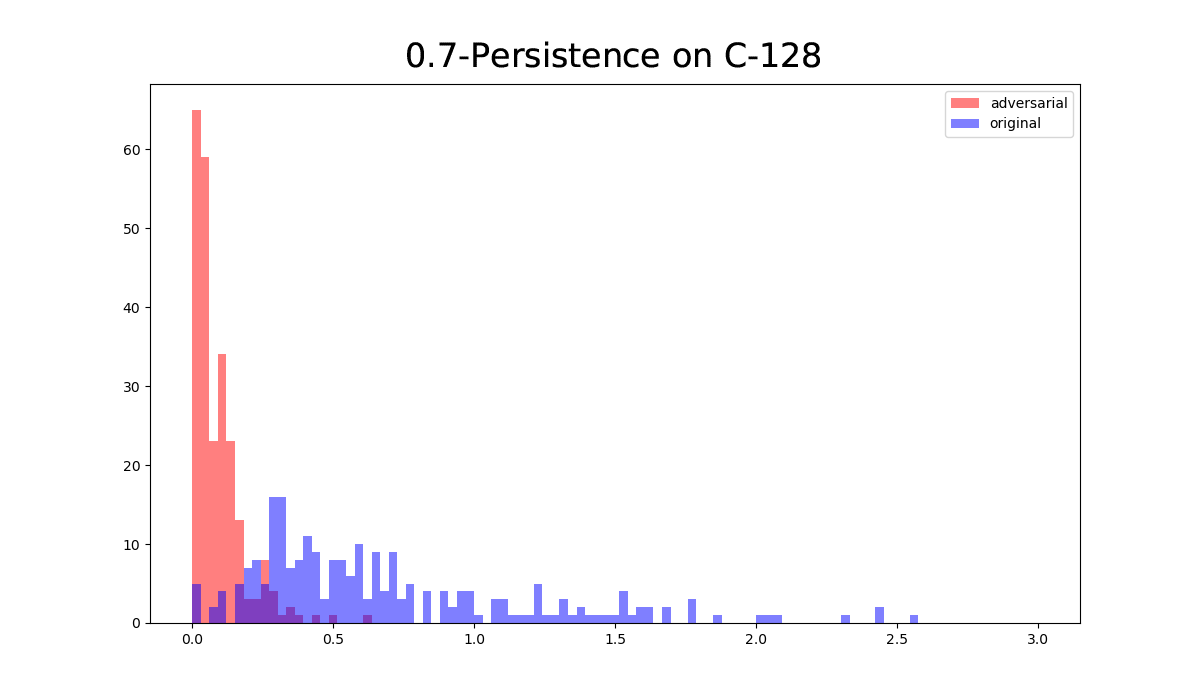
\includegraphics[width=.49\textwidth]{c3_figures/MNIST-C-128-0-stab_compare_a_var-hist.png}
% 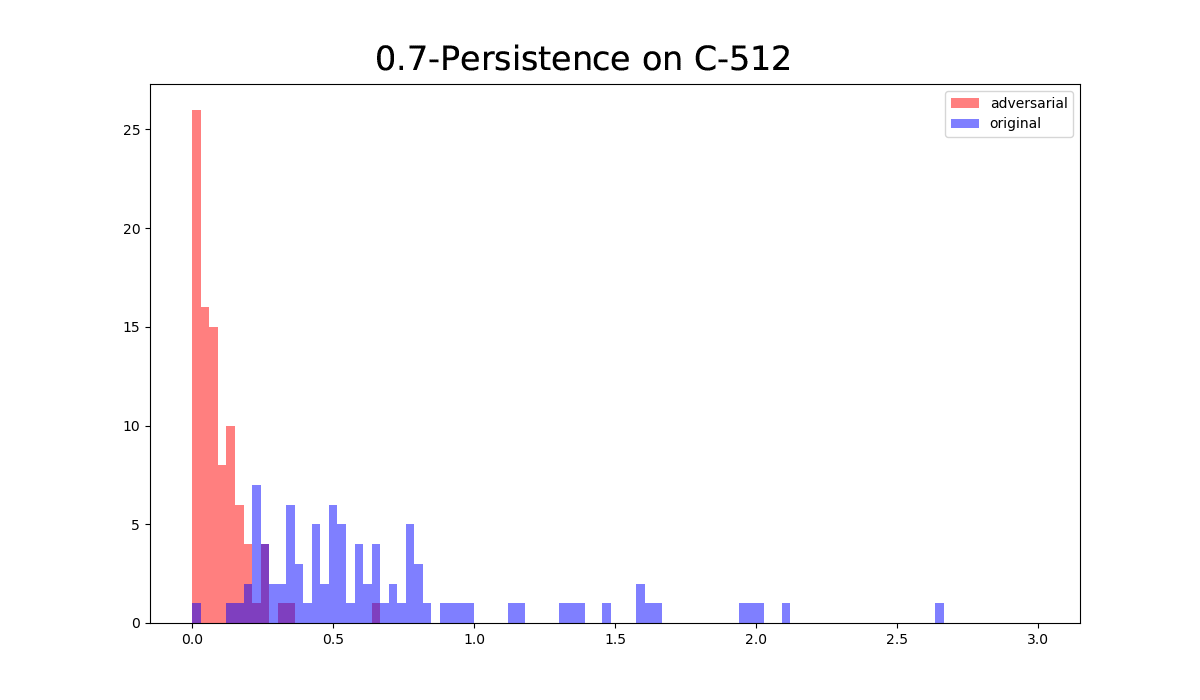
\includegraphics[width=.49\textwidth]{c3_figures/MNIST-C-512-0-stab_compare_a_var-hist.png}
% \caption{Histograms of $0.7$-persistence for C-4 (top left), C-32 (top right), C-128 (bottom left), and C-512 (bottom right) from Table \ref{table1}. Natural images are in blue and adversarial images are in red.}
% \label{fig:CNNs}
% \end{figure}

% \subsection{Additional figures for ImageNet}

% In this section we show some additional figures of Gaussian sampling for ImageNet. In Figure \ref{fig:moreimagenet} we see Gaussian sampling of an example of the class \texttt{indigo\_bunting} and the frequency samplings for adversarial attacks of \texttt{goldfinch} toward \texttt{indigo\_bunting} (classifier: alexnet, attack: PGD) and  toward  \texttt{alligator\_lizard} (classifier: vgg16, attack: PGD). Compare the middle image to Figure \ref{fig:imagenet_adv}, which is a similar adversarial attack but used the vgg16 network classifier and the BIM attack. Results are similar. Also note that in each of the cases in Figure \ref{fig:moreimagenet} the label of the original natural image never becomes the most frequent classification when sampling neighborhoods of the adversarial example. 

% \begin{figure}[!htb]
%     \centering
%     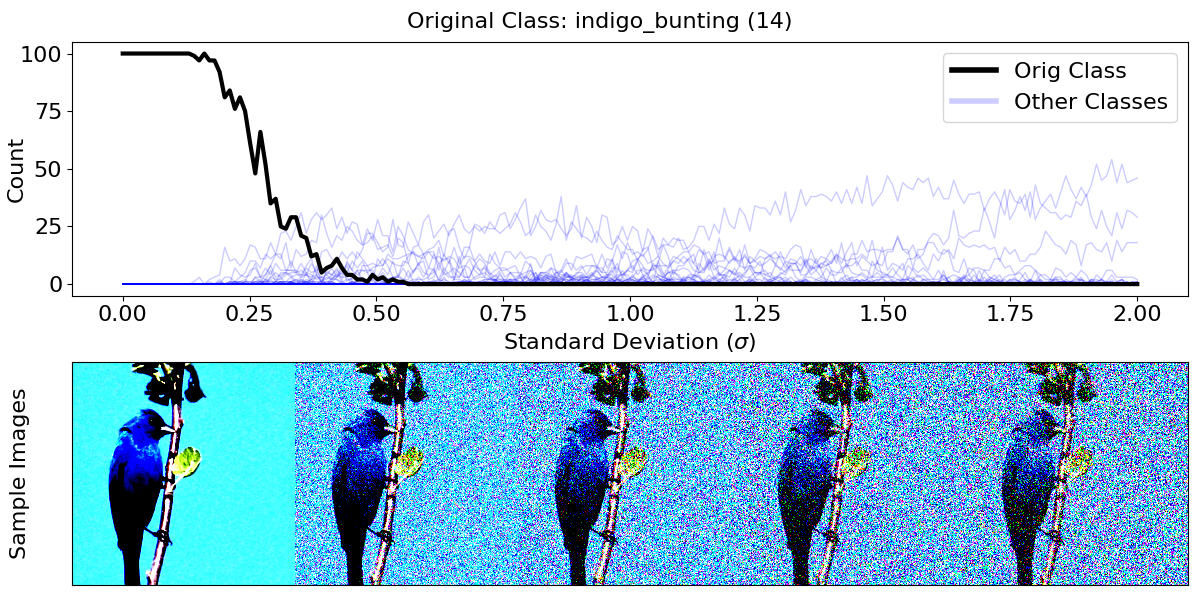
\includegraphics[width=.32\textwidth]{c3_figures/ILSVRC2012_val_00000414-vgg16-sampling.png}
%     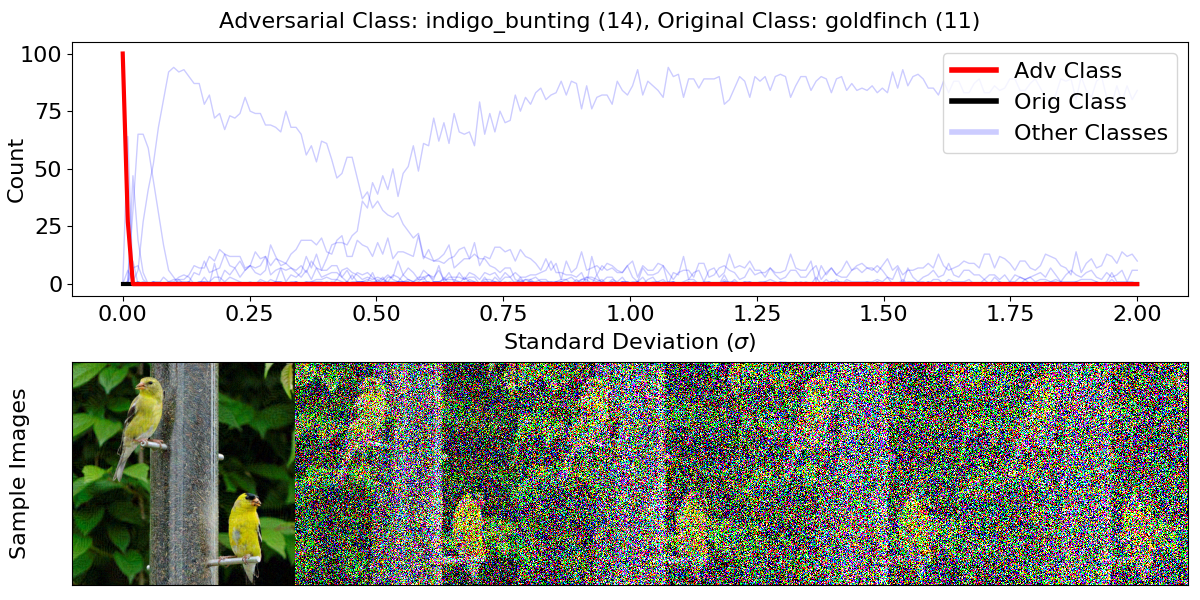
\includegraphics[width=.32\textwidth]{c3_figures/IMNET-class-11-alexnet-PGD-48-attack_data-023.png}
%     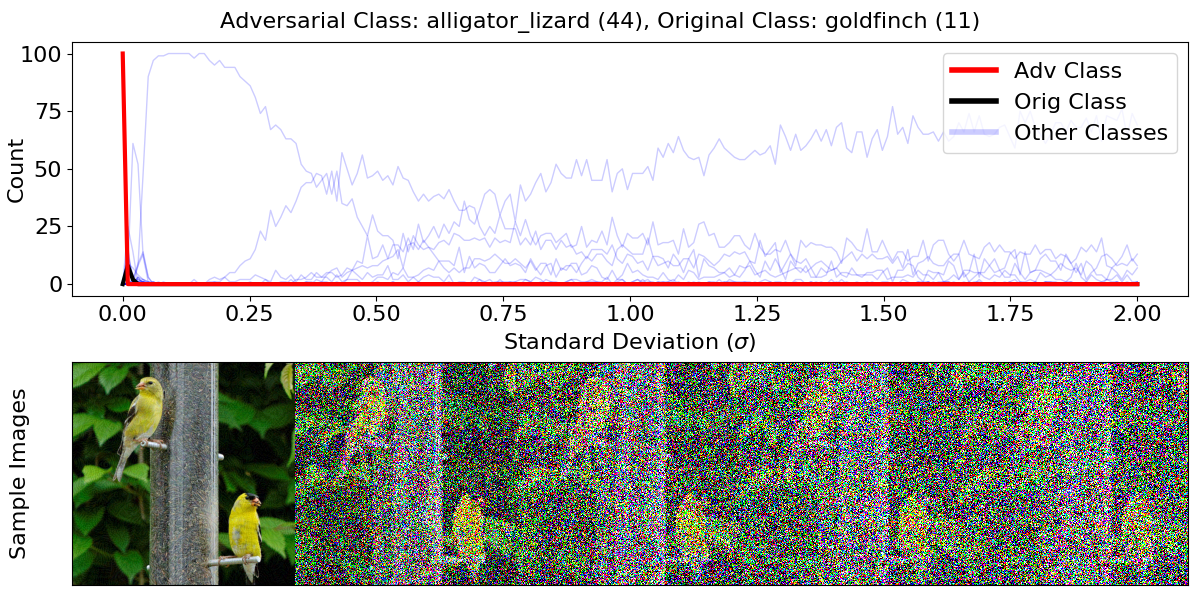
\includegraphics[width=.32\textwidth]{c3_figures/IMNET-class-11-vgg16-PGD-48-attack_data-039.png}
%     \caption{Frequency of each class in Gaussian samples with increasing variance around an \texttt{indigo\_bunting} image (left), an adversarial example of the image in class \texttt{goldfinch} from Figure \ref{fig:imagenet_adv} targeted at the \texttt{indigo\_bunting} class on a alexnet network attacked with PGD (middle), and an adversarial example of the \texttt{goldfinch} image targeted at the \texttt{alligator\_lizard} class on a vgg16 network attacked with PGD (right). Bottoms show example sample images at different standard deviations.}
%     \label{fig:moreimagenet}
% \end{figure}


% In Figure \ref{fig:persistencediffgamma}, we have plotted $\gamma$-persistence along a straight line from a natural image to an adversarial image to it with differing values of the parameter $\gamma$. The $\gamma$-persistence in each case seems to change primarily when crossing the decision boundary. Interestingly, while the choice of $\gamma$ does not make too much of a difference in the left subplot, it leads to more varying persistence values in the right subplot of Figure \ref{fig:persistencediffgamma}.  This suggests that one should be careful not to choose too small of a $\gamma$ value, and that persistence does indeed depend on the landscape of the decision boundary described by the classifier.

% \clearpage
% \begin{figure}[!htb]
%     \centering
%     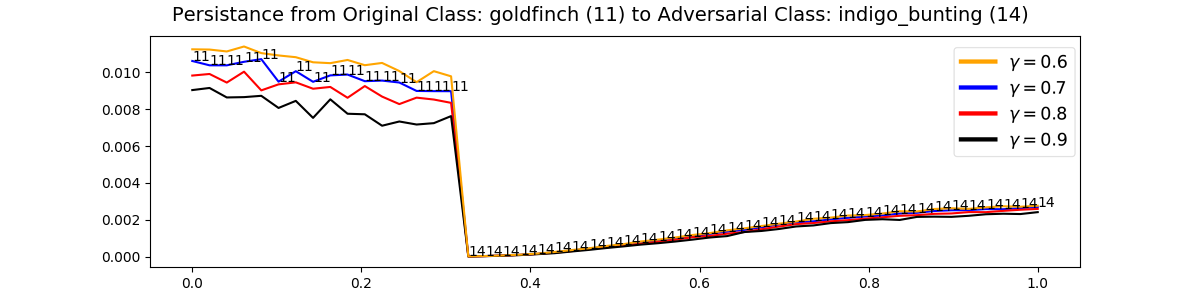
\includegraphics[width=.49\textwidth]{c3_figures/persistence_interpolation-multi-sigma-IMNET-class-11-vgg16-BIM-48-attack_data-001.png}
%     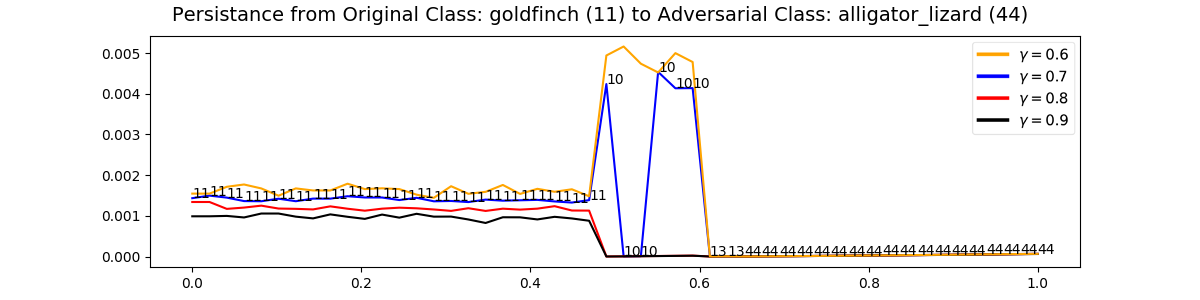
\includegraphics[width=.49\textwidth]{c3_figures/persistence_interpolation-multi-sigma-IMNET-class-11-vgg16-PGDL2-1008-attack_data-003.png}
% %    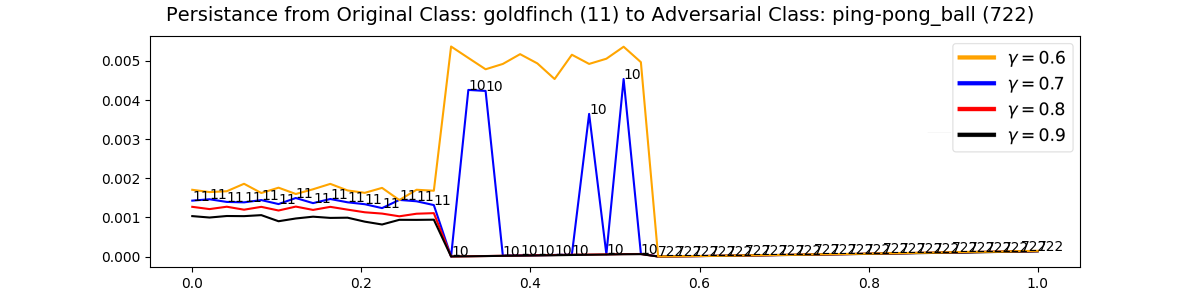
\includegraphics[width=.32\textwidth]{persistence_interpolation-multi-sigma-IMNET-class-11-vgg16-PGDL2-1008-attack_data-005}
%     \caption{The $\gamma$-persistence of images along the straight line path from an image in class \texttt{goldfinch} (11) to an adversarial image generated with BIM in the class \texttt{indigo\_bunting} (14)  (left) and to an adversarial image generated with PGL in the class \texttt{alligator\_lizard} (44) (right) on a vgg16 classifier with different values of $\gamma$. The classification of each image on the straight line is listed as a number so that it is possible to see the transition from one class to another. The vertical axis is $\gamma$-persistence and the horizontal axis is progress towards the adversarial image.}
%     \label{fig:persistencediffgamma}
% \end{figure}


% \section{Concentration of measures} \label{sec:concentration}

% We use Gaussian sampling with varying standard deviation instead of sampling the uniform distributions of balls of varying radius, denoted $U(B_r(0))$ for radius $r$ and center $0$. This is for two reasons. The first is that Gaussian sampling is relatively easy to do. The second is that the concentration phenomenon is different. This can be seen in the following proposition.

% \begin{proposition} \label{prop:concentration}
%     Suppose $x \sim N(0,\sigma^2 I)$ and $y \sim U(B_r(0))$ where both points come from distributions on $\RR^n$. For $\varepsilon < \sqrt{n}$ and for $\delta < r$ we find the following:
%     \begin{align}
%         \mathbb{P}\left[\rule{0pt}{15pt} \left| \rule{0pt}{10pt} \Norm{x} - \sigma \sqrt{n} \right| \leq \varepsilon \right] &\geq 1-2e^{-\varepsilon^2/16} \\
%         \mathbb{P}\left[\rule{0pt}{15pt} \left| \rule{0pt}{10pt} \Norm{y} - r \right| \leq \delta \right] &\geq 1-e^{-\delta n/r} 
%     \end{align}
% \end{proposition}
% \begin{proof}
%     This follows from \cite[Theorems 4.7 and 3.7]{wegner2021lecture}, which are the Gaussian Annulus Theorem and the concentration of measure for the unit ball, when taking account of varying the standard deviation $\sigma$ and radius $r$, respectively.
% \end{proof}

% The implication is that if we fix the dimension and let $\sigma$ vary, the measures will always be concentrated near spheres of radius $\sigma \sqrt{n}$ and $r$, respectively, in a consistent way. In practice, Gaussians seem to have a bit more spread, as indicated in Figure \ref{fig:sampling}, which shows the norms of $100,000$ points sampled from dimension $n=784$ (left, the dimension of MNIST) and $5,000$ points sampled from dimension $n=196,608$ (right, the dimension of ImageNet).

% \begin{figure}[htb]
%     \centering
%     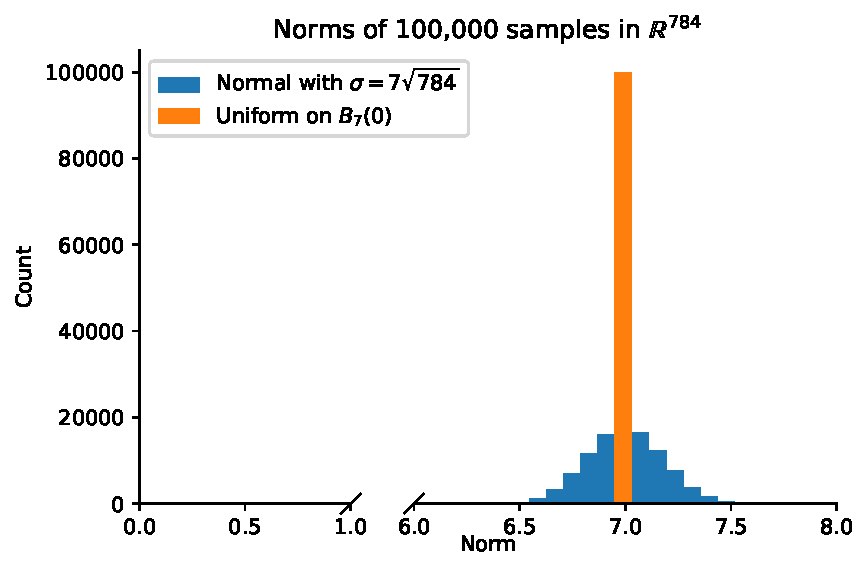
\includegraphics[width=.5\textwidth]{./c3_figures/mnistsample.pdf}
%     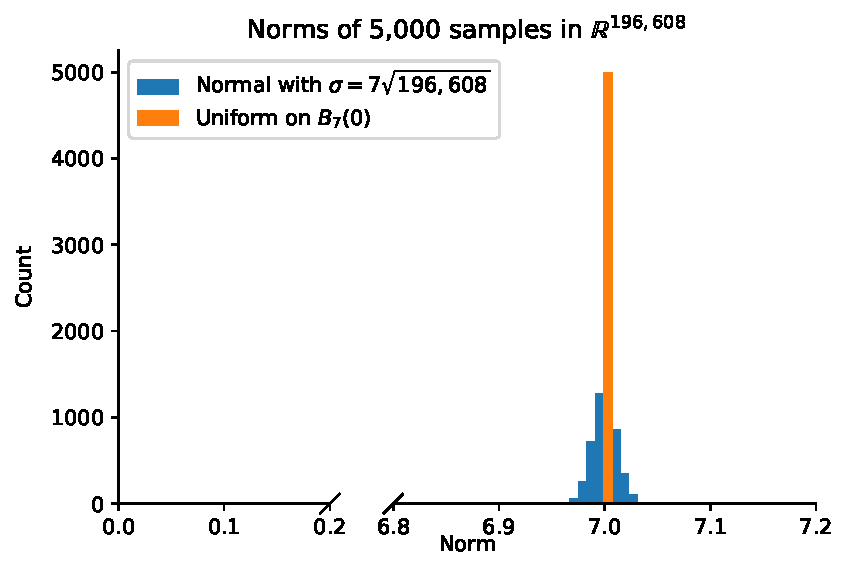
\includegraphics[width=.48\textwidth]{./c3_figures/imagenetsample.pdf}
%     \caption{Comparison of the length of samples drawn from $U(B_7(0))$ and $N(0,7\sqrt{n})$ for $n=784$, the dimension of MNIST, (left) and $n=196,608$, the dimension of ImageNet, (right).}
%     \label{fig:sampling}
% \end{figure}

% %Technically, it only shows one side of the bound so maybe it is not true???

% %{\color{red}[K]?? So this shows that sampling via Gaussians about a data point is essentially sampling a thin annulus about the sphere of radius $\sigma\sqrt{n}$ centered at $x$.  This may mean that if we look for proportional "volume" from Gaussian sampling, we are really looking more at proportional surface area on the sphere. Could it be that this fraction is better behaved than looking at the volume fraction of the ball?  As a counterpoint though, the argument from \citet{inevitable2018} might indicate that it's not any better behaved.}

% %{\color{blue}[DG]: I think the takeaway is that looking at balls and looking at Gaussians is almost the same as long as the radii are not too small and not too large, since in this case it affects the estimates. However, it is a one sided bound so maybe it is just affecting the estimate and not the actual behavior. It probably would be good to do some numerical experiments with Gaussians of high dimension like those in \cite[Figure 1.4]{wegner2021lecture}}

% %The following is wrong. I think these two distributions are exactly the same!
% %We can also look at the difference between considering perturbations of the form $y=x+ \varepsilon \triangle x$ where $\triangle x \sim N({\bf 0},1)$ and perturbations of the form $z$ where $z \sim N(x, \sigma^2 I)$. If we take $\varepsilon=\sigma$, we find that the expected length of the new vectors is the same, i.e., 
% % \begin{align*}
% %     \mathbb{E} [|y|] &= x+  \frac{\varepsilon}{(\sqrt{2\pi})^n}\int_{\RR^n} |y|e^{\frac{|y-x|^2}{2}}dy\\
% %     &= \frac{\varepsilon}{(\sqrt{2\pi})^n}\int_{\RR^n} |w+x|e^{\frac{|w|^2}{2}}dw
% % \end{align*}
% % and 
% % \begin{align*}
% % \mathbb{E} [|z|] &= \frac{1}{(\sqrt{2\pi}\sigma)^n}\int_{\RR^n} |z|e^{\frac{|z-x|^2}{2\sigma^2}}dz \\
% % &= \frac{1}{(\sqrt{2\pi})^n}\int_{\RR^n} |\sigma w+x|e^{\frac{|w|^2}{2}}dw.
% % \end{align*}

% % However, a similar calculation shows that 
% % \[
% %  \mathbb{E} \left[(|z|-\mathbb{E} [|z|])^2\right] = \sigma \mathbb{E} \left[(|y|-\mathbb{E} [|y|])^2\right]. 
% % \]
% % DG: I don't think I see this in the sampling...

% \section{Licenses of Assets}

% We acknowledge the use of the following licensed materiasl: PyTorch (BSD License), MNIST (CC BY-SA 3.0 License), Imagenet (No License -- downloaded in accordance with Princeton and Stanford University terms of access), and TorchAttacks (MIT License).

\section{Conclusion}

%In general, our intuition that adversarial examples are less stable than than natural examples is supported by the results in Table \ref{table1}. 


%The more complex neural networks tended to support less stable adversarial examples, but ones that are closer to the natural examples. 


In order to better understand the observed tendency for points near natural data to be classified similarly and points near
adversarial examples to be classified differently, we defined a notion of $(\gamma,\sigma)$-stability which is easily estimated by Monte Carlo sampling. For any data point $x$, we then define the $\gamma$-persistence to to be the smallest $\sigma_\gamma$ such that the probability of similarly classified data is at least $\gamma$ when sampling from Gaussian distributions with mean $x$ and standard deviation less than $\sigma_\gamma$. The persistence value can be quickly estimated by a Bracketing Algorithm. These two measures were considered with regard to both the MNIST and ImageNet datasets and with respect to a variety of classifiers and adversarial attacks. We found that adversarial examples were much less stable than natural examples in that the $0.7$-persistence for natural data was usually significantly larger than the $0.7$-persistence for adversarial examples. We also saw that the dropoff of the persistence tends to happen precisely near the decision boundary. Each of these observations is strong evidence toward the hypothesis that adversarial examples arise inside cones or high curvature regions in the adversarial class, whereas natural images lie outside such regions.

We also found that often the most likely class for perturbations of an adversarial examples is a class other than the class of the original natural example used to generate the adversarial example; instead, some other background class is favored. In addition, we found that some adversarial examples may be more stable than others, and a more detailed probing using the concept of $(\gamma,\sigma)$-stability and the $\gamma$-persistence statistic may be able to help with a more nuanced understanding of the geometry and curvature of the decision boundary. Although not pursued here, the observations and statistics used in this paper could potentially be used to develop methods to detect adversarial examples as in \cite{crecchi2019,frosst2018,hosseini2019odds,Lee2018ASU,qin2020,roth19aodds} and others. As with other methods of detection, this may be susceptible to adaptive attacks as discussed by ~\cite{tramer2020adaptive}. 





